\documentclass{article}
\usepackage[utf8]{inputenc}
\usepackage{parskip}
\usepackage{tikz}
\usepackage{atbegshi}
\usepackage{csquotes}
\usetikzlibrary{decorations.markings, calc, arrows.meta, hobby, intersections, decorations.pathreplacing, calligraphy, patterns}
\usepackage{pifont}
\usepackage[labelfont=bf, textfont=it]{caption}
\usepackage{amssymb, amsfonts, amsthm}
\usepackage[lightmath]{kpfonts}
\let\kpfontsRe\Re
\let\kpfontsIm\Im
\usepackage{physics}
\usepackage[fixamsmath]{mathtools}
\renewcommand{\Re}{\kpfontsRe}
\renewcommand{\Im}{\kpfontsIm}
\usepackage{cancel}
\usepackage{esint}
\usepackage{graphicx}
\usepackage[english]{babel}
\usepackage{xparse}
\usepackage{enumitem}
\usepackage{pgfplots}
\usepackage{stackengine}
\usepackage{scalerel}
\stackMath

\usepackage[inkscapelatex=false]{svg}
\pgfplotsset{width=10cm,compat=1.9}

\setlist[enumerate]{label=(\arabic*)}
\setlist[itemize]{label=\ding{226}}

\usepackage{hyperref}
\usepackage[backend=biber, style=alphabetic, sorting=ynt]{biblatex}
\addbibresource{references.bib}
\nocite{*}

\everymath{\displaystyle}

\allowdisplaybreaks[2]

\newcommand{\tikzhalflengtharrow}[2]{%
    \path (#1) -- (#2) coordinate[pos=0.25] (Pstart) coordinate[pos=0.75] (Pend);
    \draw[-{Stealth}, thick, black] (Pstart) -- (Pend);
}

\newcommand{\ddx}{\dd{x}}
\newcommand{\ddy}{\dd{y}}
\newcommand{\ddz}{\dd{z}}
\newcommand{\ddzeta}{\dd{\zeta}}
\newcommand{\ddt}{\dd{t}}
\newcommand{\supp}{\operatorname{supp}}
\newcommand{\Log}{\mathrm{Log}}
\newcommand{\Arg}{\mathrm{Arg}}
\newcommand{\Aut}{\mathrm{Aut}}

\newtheorem{theorem}{Theorem}[section]
\newtheorem{corollary}{Corollary}[theorem]
\newtheorem{lemma}{Lemma}[section]
\theoremstyle{remark}
\newtheorem{example}{Example}[subsection]
\theoremstyle{definition}
\newtheorem{definition}{Definition}[section]
\theoremstyle{remark}
\newtheorem*{remark}{Remark}
\providecommand*{\lemmaautorefname}{Lemma}
\providecommand*{\definitionautorefname}{Definition}
\providecommand*{\corollaryautorefname}{Corollary}
\providecommand*{\exampleautorefname}{Example}
\numberwithin{equation}{subsection}
\numberwithin{figure}{section}
\DeclarePairedDelimiter{\paren}{(}{)}
\let\parendefault\paren%
\renewcommand{\paren}{\parendefault*}
\DeclarePairedDelimiter{\brackets}{[}{]}
\let\bracketsdefault\brackets%
\renewcommand{\brackets}{\bracketsdefault*}
\DeclarePairedDelimiter\ceil{\lceil}{\rceil}
\let\ceildefault\ceil%
\renewcommand{\ceil}{\ceildefault*}
\DeclarePairedDelimiter\floor{\lfloor}{\rfloor}
\let\floordefault\floor%
\renewcommand{\floor}{\floordefault*}

\NewDocumentCommand{\cbraces}{m g}{\ensuremath{\left\lbrace#1\IfNoValueTF{#2}{}{\,\middle|\,#2}\right\rbrace}}

\newcommand{\extcomplex}{\widehat{\mathbb{C}}}
\newcommand{\ee}{\mathrm{e}}
\newcommand{\ii}{\mathrm{i}}
\newcommand{\chpref}[1]{\hyperref[#1]{\S\ref*{#1}}}
\newcommand{\interior}[1]{\overset{\circ}{#1}}
\newcommand{\doubletilde}[1]{
    \rlap{\raisebox{0.45ex}{$\widetilde{\phantom{#1{}}}$}}%
    \widetilde{#1{}}
}

\DeclareMathOperator*{\residue}{Res}
\makeatletter
\renewcommand{\@pnumwidth}{1.65em} 
\renewcommand{\@tocrmarg}{2.2em} 
\makeatother

\title{Complex Analysis}
\author{Slipper King}
\date{May 2025}
\begin{document}
\maketitle
\tableofcontents
Made with \LaTeX.

{\newcommand{\rep}[1]{{#1}^{#1}_{#1}}

    \newcommand{\rrep}[2]{%
        \ifnum#1>0
        \expandafter\rrep\expandafter{\number\numexpr#1-1\relax}{\rep{#2}}%
        \else
        #2%
        \fi
    }
    \AtBeginShipoutUpperLeft{%
    \tikz[overlay,remember picture] 
        \node[anchor=north west,scale=3,gray] at (current page.north west) {\makebox[0pt][l]{\(\smash{\textcolor{lightgray}{\rrep{7}{\textstyle\int}}}\)}};%
    }
    %\hspace*{-1in}\hspace*{-\oddsidemargin}\makebox[0pt][l]{\(\smash{\textcolor{lightgray}{\rrep{7}{\textstyle\int}}}\)}
}\newpage
\section{Prerequisites}
\subsection{Topological Preliminaries}
We will provide a rough, informal notion of important topological concepts tailored specifically towards complex analysis.
\begin{definition}[Accumulation Point]\label{def:accumulationpoint}
    A point \(z\in\mathbb{C}^n\) is an \textit{accumulation point} of \(X\) if for any open set \(U\) containing \(z\), \((U\setminus\{z\})\cap X\neq\emptyset\)
\end{definition}
\begin{definition}[Closure]\label{def:closure}
    For a set \(X\in\mathbb{C}^n\), define the \textit{closure} of \(X\), or \(\overline{X}\) to be the intersection of all closed sets containing \(X\). In other words, it is the union of \(X\) and its accumulation points.
\end{definition}
\begin{definition}[Interior]\label{def:interior}
    For a set \(X\in\mathbb{C}^n\), the \textit{interior} of \(X\), denoted \(\interior{X}\), is the union of all open sets contained in \(X\), or the set of points \(z\in\mathbb{C}^n\) such that there exists an open neighborhood of \(z\) that is fully contained in \(X\).
\end{definition}
\begin{definition}[Compact Set]\label{def:compactsets}
    A set \(X\in\mathbb{C}^n\) is compact if and only if \(X\) is closed and bounded.
\end{definition}
\begin{definition}[Cover of a Set]
    A cover \(\mathcal{C}\) of a set \(X\) is a collection of sets \(\cbraces{U_n}\) such that \[\bigcup_{n\in\mathbb{N}}U_n\supseteq X.\] A cover is \textit{open} if every set in the collection is open.
\end{definition}
\begin{theorem}[Bolzano--Weierstrass Theorem]\label{thm:bolzanoweierstrass}
    Every infinite subset \(A\) of a compact set \(X\subset\mathbb{C}^n\) has an accumulation point in \(X\).
\end{theorem}
\begin{proof}
    Since \(X\) is bounded, there exists a closed cube \(Q\subset\mathbb{C}^n\) such that \(A\subseteq X\subset Q\).

    Bisect \(Q_0=Q\) into \(2^{2n}\) congruent sub-cubes. Since \(A\) is infinite and the sub-cubes are finite in number, at least one of the sub-cubes contains infinitely many points of \(A\), and choose one to be \(Q_1\).

    Bisect \(Q_1\) into \(2^{2n}\) sub-cubes, and choose a sub-cube \(Q_2\subset Q_1\) that contains infinitely many points of \(A\). We then obtain the recursive sequence \[Q_0\supset Q_1 \supset Q_2\supset\cdots.\]

    Because the side lengths shrink to zero and the cubes are nested, the intersection
    \[\bigcap_{k=0}^{\infty} Q_k\]
    consists of exactly one point. Call this point \(z_\infty\in\mathbb{C}^n\).

    For each \(k\), \(Q_k\) contains infinitely many points of \(A\). Because the side length of \(Q_k\) tends to zero, for any \(\varepsilon>0\), \(\exists N\in\mathbb{N}\) such that \(\forall k\geq N\), \(Q_k\subset B^n(z_\infty,\varepsilon)\) where \(B^n(a,r)\subset\mathbb{C}^n\) is the \(n\)-dimensional \textit{ball} with radius \(r\) centered at \(a=\paren{a_1,a_2,\ldots,a_n}\in\mathbb{C}^n\), or \[B^n(a,r)=\cbraces{\qty(z_1,z_2,\ldots,z_n)\in\mathbb{C}^n}{\sum_{j=1}^n\abs{z_j-a_j}^2<r^2}.\]
    Then, \(B^n(z_\infty, \varepsilon)\) also contains infinitely many points of \(A\). Therefore, \(z_\infty\) is an accumulation point of \(A\).

    We now show that \(z_\infty\in X\). Suppose for contradiction that \(z_\infty\notin X\). Since \(X\) is closed, \(\mathbb{C}^n\setminus X\) is open, and \(\exists\delta>0\) such that \[B^n(z_\infty,\delta)\subset\mathbb{C}^n\setminus X.\] But then, for sufficiently large \(k\), we have \(Q_k \subset B^n(z_\infty, \delta)\), and hence \(Q_k\cap X=\emptyset\). This contradicts the construction of \(Q_k\), which ensures that \(Q_k\) contains infinitely many points of \(A \subset X\).
\end{proof}
\begin{theorem}[Heine--Borel]\label{thm:heineborel}
    A set \(X\in\mathbb{C}^n\) is compact if and only if every open cover has a finite subcover.
\end{theorem}
\begin{proof}
    We will first show that any set satisfying the condition is compact.

    First we will show that \(X\) is bounded. Suppose that \(\forall R>0\), \(\exists z\in X\) where \(\norm{z}>R\). Consider the collection of open sets \[\mathcal{U}=\{B^n(0,k)\mid k\in\mathbb{N}\}.\] \(\mathcal{U}\) forms an open cover of \(X\). Then by the assumption, there exists a finite subcover in \(\mathcal{U}\), namely \(\{B^n(0,k_1),\ldots,B^n(0,k_m)\}\) which covers \(X\). Then, \[X\subseteq\bigcup_{i=1}^mB^n(0,k_i)=B^n(0,\max(k_1,\ldots k_m)).\] By contradiction, \(X\) must be bounded.

    \(X\) must also be a closed set. For the sake of contradiction, assume that there exists a point \(z_0\in\overline{X}\setminus X\). Since \(z_0\notin X\), the following open collection of sets covers \(X\):
    \[\mathcal{U}=\left\{\mathbb{C}^n\setminus\overline{B^n\qty(z_0,\frac{1}{k})}\;\middle|\; \forall k\in\mathbb{N}\right\}.\]
    There then exists a finite subcover \(\mathcal{C}=\left\{\mathbb{C}^n\setminus\overline{B^n\qty(z_0,\frac{1}{k_i})}\;\middle|\; i=1,2,\ldots,m\right\}\). Then, \[X\subseteq\mathbb{C}^n\setminus\overline{B^n\qty(z_0,\frac{1}{\max(k_1,\ldots,k_m)})},\]
    and that \(X\cap\overline{B^n\qty(z_0,\frac{1}{\max(k_1,\ldots,k_m)})}=\emptyset\). However, by the definition of the accumulation point, every open neighborhood of the accumulation point must intersect \(X\). Therefore, by contradiction, \(X\) is closed.

    We then prove the converse. By the assumption that \(X\) is bounded, \(\exists R>0\) such that the \(X\) is contained within the closed cube \[Q=\cbraces{z\in\mathbb{C}^n}{\max_{i\in\{1,\ldots,n\}}\abs{\Re(z_i)}\le R,\max_{i\in\{1,\ldots,n\}}\abs{\Im(z_i)}\le R}.\]

    Assume that there exists an infinite open cover \(\mathcal{U}\) of \(X\) without finite subcovering. Bisect \(Q_0=Q\) into \(2^{2n}\) sub-cubes (for real and complex parts). Choose \(Q_1\) such that \(Q_1\cup X\) has no finite subcover of \(\mathcal{U}\). Under the previous assumptions, this is possible since if every \(\text{sub-cube}\cap X\) had finite subcovering, then \(Q_0\cap X=X\) would have finite subcovering. Similarly, choose \(Q_2\) by bisecting \(Q_1\) in a similar way, and recursively obtain a sequence of cubes:
    \[Q_0\supset Q_1\supset Q_2\supset\ldots\]
    Since the side length of each cube tends to 0, \(\bigcap_{i=0}^\infty Q_i\) consists of a single point \(z_{\infty}\in\mathbb{C}^n\). By the Bolzano-Weierstrass Theorem (\autoref{thm:bolzanoweierstrass}), because \(\forall i\in\mathbb{N}\), \(Q_i\cap X\neq\emptyset\), select a point \(z_{i}\in Q_i\cap X\), forming a sequence \({z_k}\in X\) convergent to \(z_\infty\in X\) as \(X\) is closed. Therefore, \(\exists U\in\mathcal{U}\) where \(z_\infty\in U\). Since \(U\) is open, \(\exists\varepsilon>0\) such that \(B^n(z_\infty,\varepsilon)\subset U\).\ \(\exists N\in\mathbb{N}\) such that \(\forall k>N\), \(Q_k\subset B^n(z_\infty,\varepsilon)\). Then taking the intersection with \(X\) on both sides, \[Q_k\cap X\subseteq B^n(z_\infty,\varepsilon)\cap X\subset U.\] Our original assumption said that for every \(k\), \(Q_k\cap X\) has no finite subcovering. However, \(U\) covers \(Q_k\cap X\), which is a single open set that covers a nonempty subset. Therefore by contradiction, every open cover has finite subcovering.
\end{proof}
\begin{definition}[Support of a Function]\label{def:support}
    For a set \(X\) and a function \(f:X\to\mathbb{C}\), the \textit{support}, denoted by \(\supp(f)=\overline{\{z\in X\mid f(z)\neq 0\}}\), is the closure of the set for which \(f\) is nonzero.
\end{definition}
\begin{remark}
    We are primarily concerned when the support of a function is compact, or if the support is bounded. Functions that are compactly supported and \(C^\infty\) are also called \textit{bump functions}.
\end{remark}
\subsection{Calculus}
Since traditional complex analysis is the theory of calculus on complex functions, it is only natural that generalizations are made on classical formulas in calculus for complex functions.

It is well known that a function \(f:(a,b)\to\mathbb{R}\) is differentiable at a point \(x\in(a,b)\) if the limit \[\lim_{h\to0}\frac{f(x+h)-f(x)}{h}\] exists, and the value of this limit is the derivative of \(f(x)\), denoted by \(f'(x)\) or \(\frac{\dd{f}}{\ddx}\). The value \(\dd{f}=f'(x)\ddx\) is the differential of \(f(x)\). Partition \([a,b]\) into \(a=x_0<x_1<x_2<\cdots<x_n=b\) such that the length of the intervals \([x_i,x_{i-1}]\) tends to 0 as \(n\to\infty\). If for any such partition, the sum \[\sum_{i=1}^n f(\xi_i)(x_i-x_{i-1})\] tends to the same value \(\forall\xi_i\in[x_{i-1},x_i]\), then the function can be roughly said to be integrable over \([a,b]\). The full details of Riemann integrability relate to the upper and lower Riemann sums and will not be discussed here. The value of this sum is denoted by \[\int_a^bf(x)\dd{x}.\] The following theorems are the fundamental results of classical calculus:
\begin{theorem}[Fundamental Theorem of Calculus, Differential Form]
    Let \(f(x)\) be a function continuous over \([a,b]\). For \(x\in[a,b]\), define
    \[\Phi(x)=\int_a^x f(t)\dd{t}.\]
    Then \(\Phi(x)\) is differentiable over \([a,b]\), \(\Phi'(x)=f(x)\), and \(\dd{\Phi(x)}=f(x)\dd{x}\).
\end{theorem}
\begin{theorem}[Fundamental Theorem of Calculus, Integral Form]
    Let \(\Phi(x)\) be a function differentiable over \([a,b]\). Let \(f(x)=\Phi'(x)\) over \([a,b]\). Then,
    \[\int_a^xf(t)\dd{t}=\Phi(x)-\Phi(a).\]
\end{theorem}
The two forms of the theorem show that differentiation and integration are inverse operations to each other. Operations performed for differentiating oftentimes have a corresponding inverse operation that can be done for integrating. For instance, \[\dv{(f(x)\pm g(x))}{x}=\dv{f(x)}{x}\pm\dv{g(x)}{x}\] corresponds to \[\int(f(x)\pm g(x))\ddx=\int f(x)\ddx\pm\int g(x)\ddx,\]
and \[\dv{x}(f(x)g(x))=f'(x)g(x)+f(x)g'(x)\] corresponds to \[\int f(x)g'(x)\ddx=f(x)g(x)-\int f'(x)g(x)\ddx,\] and \[\dv{f(g(x))}{x}=\dv{f(g)}{g}\cdot\dv{g(x)}{x}\] corresponds to \[\int_a^b f(g(x))g'(x)\ddx=\int_{g(a)}^{g(b)}f(u)\dd{u}.\] Another correspondence is the Mean Value Theorem:
\begin{theorem}[Mean Value Theorem, Differential Form]
    If \(f(x)\) is differentiable over \([a,b]\), then \(\exists c\in[a,b]\) such that \[f(b)-f(a)=f'(c)(b-a).\]
\end{theorem}
\begin{theorem}[Mean Value Theorem, Integral Form]
    If \(f(x)\) is continuous over \([a,b]\), then \(\exists \xi\in[a,b]\) such that \[\int_a^b f(x)\ddx=f(\xi)(b-a).\]
\end{theorem}
A curve is a one-dimensional manifold embedded within a higher dimensional space. They can be parameterized with a vector \(\va{F}(t)=\qty(P(t),Q(t),R(t))\) of one parameter. In the complex plane, a curve is a complex-valued function \(\gamma(t)\) for a real parameter \(\alpha\leq t\leq\beta\). A curve is \textit{closed} if \(\gamma(\alpha)=\gamma(\beta)\). It is \textit{smooth} if it is continuously differentiable, and its direction is defined to be the direction as \(t\) increases. If it is smooth everywhere except at a finite number of points, it is \textit{piecewise smooth}. If it is of finite length, then the curve is said to be \textit{rectifiable}. Piecewise smooth curves are rectifiable. A curve is \textit{simple} if it is simple (non self-intersecting), or if \(\gamma\paren{t_1}=\gamma\paren{t_2}\) implies that \(t_1=t_2\). A simple closed curve is also called a \textit{Jordan curve}.
\begin{theorem}[Jordan Curve Theorem]\label{thm:jordancurve}
    Let \(\gamma\) be a Jordan curve in \(\mathbb{R}^2\). Then the set \(\mathbb{R}^2\setminus\gamma\) consists of exactly two connected subsets. One of them is the interior, denoted by \(\mathrm{int}(\gamma)\), and is a bounded set, while the other is the exterior, denoted by \(\mathrm{ext}(\gamma)\), which is unbounded. Both of the two sets share the common boundary \(\gamma\).
\end{theorem}
The theorem above seems trivial, but its rigorous proof in topology is extremely complex. The theorem itself can also be stated on \(\mathbb{C}\) instead of \(\mathbb{R}^2\). For a region \(U\), the boundary is denoted \(\partial U\). If the region bounded by any closed curve in \(U\) also lies in \(U\), then it is a \textit{simply connected} region. A connected region that is not simply connected is multiply connected. A region bound by 2 non-intersecting Jordan curves is doubly connected, and a region bound by \(n\) non-intersecting Jordan curves is traditionally known as \(n\)-connected (the modern topological definition differs). Lastly, any closed curve can degenerate to a single point or slit.

Generalizations of the differential and integral exist for multivariate functions. The partial differentials of \(f(x,y,z)\), \(\pdv{f}{x}\ddx\), \(\pdv{f}{y}\ddy\), and \(\pdv{f}{z}\ddz\) sum up to form the total differential, denoted by \(\dd{f}\). An important result in multivariable calculus allows the calculation of the derivatives of a definite integral with respect to its parameter.
\begin{theorem}[Leibniz Integral Rule]\label{thm:leibnizintegralrule}
    Let \(I\subset\mathbb{R}\) be open, and let \(a:I\to\mathbb{R}\) and \(b:I\to\mathbb{R}\) be differentiable on \(I\) such that \(\forall x\in I\), \(a(x)<b(x)\). Let \[U=\cbraces{(x,t)\in I\times\mathbb{R}}{a(x)\leq t\leq b(x)}.\] Suppose \(f(x,t)\) is a real-valued function on \(U\) such that \(f(x,t)\) and \(\pdv{f}{x}(x,t)\) are continuous on the set \(U\). Then the function \[F(x)=\int_{a(x)}^{b(x)}f(x,t)\dd{t}\] is differentiable on \(I\), and
    \[\dv{F}{x}=\int_{a(x)}^{b(x)}\pdv{f}{x}(x,t)\dd{t} + f(x,b(x))\dv{b}{x} - f(x,a(x))\dv{a}{x}.\]
\end{theorem}
Four main classical theorems exist, relating a function and its line integral in 2 and 3 dimensions, line and surface integrals in 2 and 3 dimensions, and the surface and volume integrals in 3 dimensions:
\begin{theorem}[Gradient Theorem]\label{thm:gradient}
    Let \(C\) be an oriented smooth curve in \(\mathbb{R}^3\) with boundary points \(A\) to \(B\). Then
    \[\int_C\pdv{f}{x} \ddx+\pdv{f}{y}\ddy+\pdv{f}{z}\ddz=f(B)-f(A).\]
\end{theorem}
\begin{theorem}[Green's Theorem]\label{thm:realgreen}
    Let \(U\) be a positively oriented, multiply connected subset of \(\mathbb{R}^2\) with a piecewise smooth oriented boundary \(\partial U\). Suppose that \(P(x,y),Q(x,y)\in C^1\paren{\overline{U}}\). Then,
    \[\oint_{\partial U} P\ddx+Q\ddy=\iint_U\paren{\pdv{Q}{x}-\pdv{P}{y}}\ddx\ddy.\]
\end{theorem}
\begin{theorem}[Stokes' Theorem]\label{thm:kelvinstokes}
    Suppose that \(S\subset\mathbb{R}^3\) is a positively oriented surface with a positively oriented, piecewise smooth boundary curve \(\partial S\). Suppose that \(P(x,y,z), Q(x,y,z), R(x,y,z)\in C^1\paren{\overline{S}}\). Then,
    \begin{align*}
        \oint_{\partial S} & P\ddx+Q\ddy+R\ddz                                                                                                    \\
        & =\iint_S\qty(\pdv{R}{y}-\pdv{Q}{z})\ddy\ddz+\qty(\pdv{P}{z}-\pdv{R}{x})\ddz\ddx+\qty(\pdv{Q}{x}-\pdv{P}{y})\ddx\ddy.
    \end{align*}
\end{theorem}
\begin{theorem}[Gauss' Theorem]\label{thm:divergencegauss}
    Suppose that \(V\subset\mathbb{R}^3\) is a positively oriented region with a positively oriented, piecewise smooth boundary surface \(\partial V\). Suppose that \(P(x,y,z), Q(x,y,z), R(x,y,z)\in C^1\paren{\overline{V}}\). Then,
    \[\oiint_{\partial V}P\ddy\ddz+Q\ddz\ddx+R\ddx\ddy=\iiint_V\qty(\pdv{P}{x}+\pdv{Q}{y}+\pdv{R}{z})\ddx\ddy\ddz.\]
\end{theorem}
In 3-dimensional \(\mathbb{R}^3\) space, define a scalar valued function to be a 0-form, a linear combination of \(\ddx\), \(\dd{y}\), and \(\dd{z}\) to be a 1-form, and a linear combination of \(\dd{y}\wedge\dd{z}\), \(\dd{z}\wedge\ddx\), and \(\dd{x}\wedge\dd{y}\) to be a 2-form, and \(\ddx\wedge\dd{y}\wedge\dd{z}\) to be a 3-form, where \(\wedge\) denotes an anti-commutative and associative product, where for any two differential forms \(\omega_1\) and \(\omega_2\)
\[\omega_1\wedge\omega_2=-\omega_2\wedge\omega_1.\]
Then consequently, for any differential form \(\omega\), \[\omega\wedge\omega=0.\]
We can generalize the operator \(\dd\) to increase the degree of a differential form. For instance,
\[\dd{f}=\pdv{f}{x}\ddx+\pdv{f}{y}\dd{y}+\pdv{f}{z}\dd{z},\]
which is the definition of the total differential. For a 1-form in 3-dimensional space, \(\omega_1=P\ddx+Q\dd{y}+R\dd{z}\), we can define the exterior derivative in a similar way:
\begin{align*}
    \dd{\omega_1} & =\dd{P}\wedge\ddx+\dd{Q}\wedge\dd{y}+\dd{R}\wedge\dd{z}                                                                                                    \\
    & =\left(\pdv{P}{x}\ddx+\pdv{P}{y}\dd{y}+\pdv{P}{z}\dd{z}\right)\wedge\ddx                                                                                   \\
    & \qquad+\left(\pdv{Q}{x}\ddx+\pdv{Q}{y}\dd{y}+\pdv{Q}{z}\dd{z}\right)\wedge\ddy                                                                             \\
    & \qquad\qquad+\left(\pdv{R}{x}\ddx+\pdv{R}{y}\dd{y}+\pdv{R}{z}\dd{z}\right)\wedge\dd{z}                                                                     \\
    & =\left(\pdv{R}{y}-\pdv{Q}{z}\right)\dd{y}\wedge\dd{z}+\left(\pdv{P}{z}-\pdv{R}{x}\right)\dd{z}\wedge\ddx+\left(\pdv{Q}{x}-\pdv{P}{y}\right)\ddx\wedge\ddy.
\end{align*}
Similarly, we can differentiate a 2-form \(\omega=P\ddy\wedge\dd{z}+Q\ddz\wedge\ddx+R\ddx\wedge\ddy\) to get:
\[\left(\pdv{P}{x}+\pdv{Q}{y}+\pdv{R}{z}\right)\ddx\wedge\ddy\wedge\ddz.\]
The two results above resemble the curl and divergence of \(\qty(P,Q,R)\). A differential form \(\omega\) is \textit{closed} if \(\dd{\omega}=0\), and is \textit{exact} if there exists \(\eta\) such that \(\omega=\dd{\eta}\).
\begin{lemma}[Poincaré Lemma]\label{lemma:poincare}
    For any differential form \(\omega\) on an open, contractible set \(U\subseteq\mathbb{R}^n\), if \(\omega\) is closed, then it is also exact.
\end{lemma}
It is true that for any set \(U\subseteq \mathbb{R}^n\), regardless of contractibility, that for a differential form \(\omega\) defined on \(U\), \(\dd\dd\omega=0\). In other words, all exact differential forms are closed.

With the same analogy, the above result means that if \(\omega\) is a 0-form, then \(\curl(\grad\omega)=0\), and if \(\omega\) is a 1-form, \(\div(\curl{v})=0\), where \(v\) is the vector of the coefficients of the basis differential forms of \(\omega\) (there are no correlations for higher degree forms since in 3-dimensional space, the highest degree possible for any differential form is 3).

Then, the Fundamental Theorem of Calculus, the Gradient Theorem, Green's, Stokes', and Gauss' Theorems can be generalized into:
\begin{theorem}[Stokes--Cartan]\label{thm:stokescartan}
    For an oriented smooth \(n\)-dimensional compact manifold \(M\) with boundary \(\partial M\), for a smooth differential \((n-1)\)-form \(\omega\) over \(\overline{M}\), \[\int_M\dd{\omega}=\int_{\partial M}\omega.\]
\end{theorem}
Real analysis is the subject dedicated to rigorously defining concepts such as limits, continuity, integrability, convergence, etc. The most widely used definition of a finite limit of a function is the language of \(\varepsilon\)--\(\delta\), which states:
\begin{definition}[Epsilon--Delta]\label{def:epsilondelta}
    Let \(f:U\to\mathbb{R}\) be a function defined over an open set \(U\subseteq\mathbb{R}\) such that \(a\) is an accumulation point of \(U\). We say that \(\lim_{x\to a}f(x)=L\) if for every \(\varepsilon > 0\), there exists \(\delta > 0\) such that for all \(x\in U\) with \(0<|x-a|<\delta\), we have \(|f(x)-L|<\varepsilon\).

    Similarly, we define the \textit{right-handed limit} \(\lim_{x\to a^+}f(x)=L\) if for every \(\varepsilon>0\), there exists \(\delta>0\) such that for all \(x\in U\) with \(0<x-a<\delta\), we have \(|f(x)-L|<\varepsilon\).

    Likewise, the \textit{left-hand limit} \(\lim_{x\to a^-}f(x)=L\) exists if for every \(\varepsilon>0\), there exists \(\delta>0\) such that for all \(x\in U\) with \(-\delta<x-a<0\), we have \(|f(x)-L|<\varepsilon\).
\end{definition}
We also have the definition of the limit of a sequence:
\begin{definition}[Epsilon--N]\label{def:epsilonn}
    Let \(\qty{a_n}_{n\in\mathbb{N}}\subset\mathbb{R}\) be a sequence. If \(\exists a_\infty\in\mathbb{R}\) such that \(\forall\varepsilon>0\), \(\exists N\in\mathbb{N}\) such that \(\forall n>N\), \(\abs{a_n-a_\infty}<\varepsilon\), then \(\qty{a_n}\) \textit{converges} to \(a_\infty\).
\end{definition}
\begin{theorem}[Cauchy Criterion]\label{thm:cauchycriterionsequenceconvergence}
    Let \(\qty{a_n}_{n\in\mathbb{N}}\subset\mathbb{R}\) be a sequence. Then \(\qty{a_n}\) is convergent if and only if \(\forall\varepsilon>0\), \(\exists N\in\mathbb{N}\) such that \(\forall n,m>N\), \(\abs{a_n-a_m}<\varepsilon\).
\end{theorem}
\begin{proof}
    Assume \(\qty{a_n}\) is convergent. Then \(\forall\varepsilon>0\), \(\exists N\in\mathbb{N}\) such that \(\forall n,m>N\), \(\abs{a_n-a_\infty}<\frac{\varepsilon}{2}\) and \(\abs{a_m-a_\infty}<\frac{\varepsilon}{2}\) for some \(a_\infty\in\mathbb{R}\). It follows that \[\abs{a_n-a_m}\leq\abs{a_n-a_\infty}+\abs{a_m-a_\infty}=\varepsilon.\]

    Conversely, \(\qty{a_n}\) is bounded (fixing \(N\), \(\forall n>N\), \(\abs{a_n-a_{N+1}}<\varepsilon\)). By the Bolzano--Weierstrass Theorem (\autoref{thm:bolzanoweierstrass}), \(\qty{a_n}_{n\in\mathbb{N}}\) has a subsequence \(\qty{a_{n_k}}_{k\in\mathbb{N}}\) that converges to \(a_\infty\). Therefore, \(\forall\varepsilon>0\), \(\exists N\in\mathbb{N}\) and \(\exists M\in\mathbb{N}\) such that \(\forall k>M\), \(n_k>N\), and \(\forall n>N\), \(\abs{a_n-a_{n_k}}<\frac{\varepsilon}{2}\) and \(\abs{a_{n_k}-a_\infty}<\frac{\varepsilon}{2}\). Then \[\abs{a_n-a_\infty}\leq\abs{a_n-a_{n_k}}+\abs{a_{n_k}-a_\infty}<\varepsilon.\] Hence, \(\qty{a_n}\) converges to \(a_\infty\).
\end{proof}
\begin{definition}[Limit Superior]\label{def:limsup}
    For a number sequence \(\qty{a_n}\subset\mathbb{R}\), if \(\exists a\in\mathbb{R}\) such that:
    \begin{enumerate}
        \item \(\forall\varepsilon>0\), \(\exists N\in\mathbb{N}\) such that \(\forall n>N\), \(a_n<a+\varepsilon\),
        \item \(\forall\varepsilon>0\), \(\forall N\in\mathbb{N}\), \(\exists n>N\) such that \(a_n>a-\varepsilon\),
    \end{enumerate}
    then the \textit{superior limit} of \(\qty{a_n}\) is \(a\), denoted by \(\varlimsup_{n\to\infty}a_n=\limsup_{n\to\infty}a_n=a\).
\end{definition}
\begin{definition}[Limit Inferior]\label{def:liminf}
    For a number sequence \(\qty{a_n}\subset\mathbb{R}\), if \(\exists a\in\mathbb{R}\) such that:
    \begin{enumerate}
        \item \(\forall\varepsilon>0\), \(\exists N\in\mathbb{N}\) such that \(\forall n>N\), \(a_n>a-\varepsilon\),
        \item \(\forall\varepsilon>0\), \(\forall N\in\mathbb{N}\), \(\exists n>N\) such that \(a_n<a+\varepsilon\),
    \end{enumerate}
    then the \textit{inferior limit} of \(\qty{a_n}\) is \(a\), denoted by \(\varliminf_{n\to\infty}a_n=\liminf_{n\to\infty}a_n=a\).
\end{definition}
\begin{lemma}
    A number sequence \(\qty{a_n}\) is convergent if and only if \(\varlimsup_{n\to\infty} a_n=\varliminf_{n\to\infty}a_n\).
\end{lemma}
\begin{proof}
    We first prove that \(a=\lim_{n\to\infty}a_n\) implies \(\varlimsup_{n\to\infty}a_n=\varliminf_{n\to\infty}a_n=a\).
    By \autoref{def:epsilonn}, \(\forall\varepsilon>0\), \(\exists N\in\mathbb{N}\) such that \(\forall n>N\), \[\abs{a_n-a}<\varepsilon\Longleftrightarrow a-\varepsilon<a_n<a+\varepsilon.\]
    Then from the first conditions of \autoref{def:limsup} and \autoref{def:liminf}, we get that \(\varlimsup_{n\to\infty}a_n\geq a\) and \(\varliminf_{n\to\infty} a_n\leq a\). By the second conditions, we get \(\varlimsup_{n\to\infty}a_n\leq a\) and \(\varliminf_{n\to\infty} a_n\geq a\). Therefore, \[\varlimsup_{n\to\infty}a_n=\varliminf_{n\to\infty}a_n.\]

    For the converse, assume \(\varlimsup_{n\to\infty}a_n=\varliminf_{n\to\infty}a_n\). Since \(\exists N_1\in\mathbb{N}\) such that \(\forall n>N_1\), \(a_n<a+\varepsilon\).\ \(\exists N_2\in\mathbb{N}\) such that \(\forall n>N_2\), \(a_n>a-\varepsilon\). Then \(\forall n>\max\qty(N_1, N_2)\), \(\qty|a_n-a|<\varepsilon\), as expected.
\end{proof}
\begin{definition}[Continuity]\label{def:continuity}
    A function \(f:U \to \mathbb{R}\), defined on an open set \(U \subseteq \mathbb{R}\) containing a point \(a \in U\), is said to be continuous at \(a\) if and only if \[\lim_{x\to a}f(x)=f(a).\]
\end{definition}
\begin{theorem}\label{thm:continuousfunctionboundedoncompact}
    Any continuous function on a compact set \(K\) is bounded on \(K\).
\end{theorem}
\begin{proof}
    Suppose for the sake of contradiction that \(f:U\to\mathbb{R}\) is continuous and unbounded on compact \(K\). Then for each \(n\in\mathbb{N}\), there exists \(x_n\in K\) such that \(|f(x_n)|>n\). The sequence \(\cbraces{x_n}\) lies in \(K\), which is compact, so by the Bolzano--Weierstrass Theorem (\autoref{thm:bolzanoweierstrass}), \(\cbraces{x_n}\) has an accumulation point in \(K\). In other words, there exists a convergent subsequence \(\cbraces{x_{n_k}}\) with \(\lim_{k\to\infty} x_{n_k}\in K\).

    Since \(f\) is continuous, \(\lim_{k\to\infty}f\qty(x_{n_k})=f\qty(\lim_{k\to\infty}x_{n_k})\), which is well-defined because \(\lim_{k\to\infty} x_{n_k}\in K\). However, this contradicts \(\qty|f\paren{x_{n_k}}|>n_k\to\infty\), hence \(f\) must be bounded on \(K\).
\end{proof}
\begin{theorem}[Extreme Value Theorem]\label{thm:extremevalue}
    A continuous function \(f(x)\) defined on a compact set \(K\) attains its infimum and supremum in \(K\).
\end{theorem}
\begin{proof}
    Assume that \(f\) never attains its supremum \(M\). Then, \(f(x)<M\). Define the auxiliary function \(\psi(x)=\frac{1}{M-f(x)}\), which is strictly positive and continuous as the denominator never reaches \(0\). By \autoref{thm:continuousfunctionboundedoncompact}, \(\psi(x)\) is bounded with some value of \(\mu>0\) satisfying \(\psi(x)\leq\mu\).\ \(f(x)\) also has the representation \(M-\frac{1}{\psi(x)}\), and therefore, \[f(x)\leq M-\frac{1}{\mu},\] which means that \(M\) is not the supremum. Similarly, assume that \(f\) never attains its infimum \(m\). Then \(f(x)>m\). Let \(\psi(x)=\frac{1}{f(x)-m}\), which is strictly positive and continuous as the denominator never reaches \(0\). By \autoref{thm:continuousfunctionboundedoncompact}, \(\psi(x)\) is bounded with some value of \(\mu>0\) satisfying \(\psi(x)\leq\mu\).\ \(f(x)\) also has the representation \(m+\frac{1}{\psi(x)}\), and therefore, \[f(x)\geq m+\frac{1}{\mu},\] which means that \(m\) is not the infimum.
\end{proof}
\begin{definition}[Uniform Continuity]\label{def:uniformcontinuity}
    A function \(f:U\to\mathbb{R}\), defined on a set \(U\subseteq\mathbb{R}\), is uniformly continuous if and only if \(\forall\varepsilon>0\), \(\exists\delta>0\) such that \(\forall x,y\in U\) where \(|x-y|<\delta\), \(\abs{f(x)-f(y)}<\varepsilon\).
\end{definition}
\begin{example}
    The function \(f(x)=\frac{1}{x}\) is not uniformly continuous over \((0,1)\).
\end{example}
\begin{proof}
    If \(\exists\varepsilon>0\) such that \(\forall\delta>0\), \(\exists x,y\in(0,1)\) satisfying both \(|x-y|<\delta\) and \(\abs{f(x)-f(y)}\geq\varepsilon\), then \(f\) is not uniformly continuous over \((0,1)\).

    Let \(\varepsilon=1\) and \[x=\frac{1}{n},\quad y=\frac{1}{n+1}.\] Then \(\forall\delta>0\), \(\exists n>1\) where \(\abs{x-y}<\delta\), since \(\lim_{n\to\infty}\left|x-y\right|=0\). Additionally, \(\abs{f(x)-f(y)}=1\geq\varepsilon\). This satisfies the negation, and thus, \(f(x)=\frac{1}{x}\) is not uniformly continuous over \((0,1)\).
\end{proof}
\begin{theorem}[Heine--Cantor]\label{thm:heinecantor}
    A continuous function on a compact set \(K\) is uniformly continuous on \(K\).
\end{theorem}
\begin{proof}
    Suppose for contradiction that \(f:K\to\mathbb{R}\) is continuous but not uniformly continuous on compact \(K\). Then \(\exists\varepsilon>0\) such that \(\forall\delta>0\), \(\exists x,y\in K\) with \(|x-y|<\delta\) and \(|f(x)-f(y)|\geq\varepsilon\).

    In particular, \(\forall n\in\mathbb{N}\), let \(\delta=\frac{1}{n}\). Then \(\exists x_n,y_n\in K\) such that \(|x_n-y_n|<\frac{1}{n}\) and \(|f(x_n)-f(y_n)|\geq\varepsilon\). Since \(K\) is compact, the sequence \(\cbraces{x_n}\) has a convergent subsequence \(x_{n_k}\to x_{n_\infty}\in K\). Because \(\qty|x_{n_k}-y_{n_k}|<\frac{1}{n_k}\to 0\), we also have \(y_{n_k}\to x_{n_\infty}\).

    By continuity, \(f(x_{n_k})\to f\paren{x_{n_\infty}}\) and \(f(y_{n_k})\to f\paren{x_{n_\infty}}\), so \(\qty|f(x_{n_k})-f(y_{n_k})|\to 0\), contradicting \(\qty|f(x_{n_k})-f(y_{n_k})|\geq\varepsilon\). Therefore, \(f\) is uniformly continuous on \(K\).
\end{proof}
A more general version of this proof can be achieved by using the Heine--Borel Theorem (\autoref{thm:heineborel}) in analogously to the proof of \autoref{thm:heinecantorfamily}.
\begin{definition}
    A function \(f\) is Lipschitz continuous over \(U\) if \(\exists M\in\mathbb{R}_{\geq0}\) such that \(\forall x,y \in U\), \(|f(x)-f(y)| \leq M|x-y|\). The smallest possible \(M\) satisfying the above condition is known as the Lipschitz constant.
\end{definition}
Lipschitz continuity is an important concept in real analysis and the theory of differential equations. It is a strong form of uniform continuity.
\begin{lemma}
    All Lipschitz continuous functions on \(U\) are uniformly continuous on \(U\).
\end{lemma}
\begin{proof}
    Let \(M>0\) be the Lipschitz constant. Then \(\forall \varepsilon>0\), let \(\delta=\frac{\varepsilon}{M}\). It then follows that \(\forall x,y\in U\) such that \(\abs{x-y}<\delta\), \(\abs{f(x)-f(y)}\leq M|x-y|<\varepsilon\).
\end{proof}
\begin{lemma}\label{lemma:c1lipschitz}
    A \(C^1\) function on a compact set \(K\) is Lipschitz continuous on \(K\).
\end{lemma}
\begin{proof}
    Let \(f:K\to\mathbb{R}\) be \(C^1\). By \autoref{thm:continuousfunctionboundedoncompact}, since \(K\) is compact and \(f'\) is continuous, \(\exists M>0\) such that \(\forall x\in K\), \(|f'(x)|\leq M\).

    By the Mean Value Theorem, \(\forall x,y\in K\), \(\exists c\) between \(x\) and \(y\) such that \(f(x)-f(y)=f'(c)(x-y)\). Then, \(|f(x)-f(y)|=|f'(c)||x-y|\leq M|x-y|\), which means \(f\) is Lipschitz continuous with Lipschitz constant less than or equal to \(M\).
\end{proof}
We will now give statements relating to operations on Riemann integrals:
\begin{lemma}\label{lemma:integralwithparameterproperties}
    Let \(f(x,u)\) be a continuous complex function on the rectangle defined by \(a\leq x\leq b\), \(\alpha\leq u\leq\beta\) (where \(a<b\), \(\alpha<\beta\)). Then,
    \begin{enumerate}
        \item For an arbitrary point \(u_0\in [\alpha,\beta]\), we have \[\lim_{u\to u_0}\int_a^b f(x,u)\ddx=\int_a^b f\qty(x,u_0)\ddx.\]
        \item The order of integration can be switched: \[\int_a^b\int_\alpha^\beta f(x,u)\dd{u}\ddx=\int_\alpha^\beta\int_a^b f(x,u)\ddx\dd{u}\]
    \end{enumerate}
\end{lemma}
\begin{proof}
    The second part is self-explanatory as it can be interpreted as an area integral.

    Let \[\varphi(u)=\int_a^b f(x,u)\ddx.\]
    Since \(f(x,u)\) is continuous on a compact set with respect to both \(x\) and \(u\), by \autoref{thm:heinecantor}, \(\forall\varepsilon>0\), \(\exists\delta>0\) such that \(\forall\qty(x_1,u_1),\qty(x_2,u_2)\in[a,b]\times[\alpha,\beta]\) satisfying \(\abs{\qty(x_1-x_2,u_1-u_2)}<\delta\), we have \(\abs{f(x_1,u_1)-f(x_2,u_2)}<\frac{\varepsilon}{b-a}\). Then for \(\abs{u-u_0}<\delta\), the integral difference can be bounded by \[\abs{\varphi(u)-\varphi\qty(u_0)}\leq\int_a^b\abs{f(x,u)-f\qty(x,u_0)}\ddx<\varepsilon.\]
\end{proof}
\section{Complex Prerequisites}
\subsection{The Complex Plane}
All complex numbers form a field that extends the real number field. A complex number \(\alpha+\ii\beta\) can be visualized on a rectangular plane as the point \((\alpha,\beta)\), with two axes: the real axis and the imaginary axis. It is well known that any complex number also has the polar form \(r\ee^{\ii\theta}=r\paren{\cos\theta+\ii\sin\theta}\).

The infinity point, \(\infty\), extends \(\mathbb{C}\) with \(\extcomplex=\mathbb{C}\cup\{\infty\}\). The following arithmetic operations are defined: \(\forall a\in\mathbb{C}\), \(a+\infty=\infty+a=\infty\), and \(\forall b\in\mathbb{C}\setminus\{0\}\), \(b\cdot\infty=\infty\cdot b=\infty\) and \(\frac{a}{\infty}=0\).

Let \(S^2=\left\{\paren{x_1,x_2,x_3}\in\mathbb{R}\,\middle|\,x_1^2+x_2^2+x_3^2=1\right\}\). There exists a \textit{stereographic projection} of \(S^2\) onto \(\extcomplex\). For every point other than \((0,0,1)\), there is a corresponding complex number
\begin{equation}\label{eq:extcomplexformula1}
    z=\frac{x_1+\ii x_2}{1-x_3}.
\end{equation}
This correspondence between \(\mathbb{C}\) and \(S^2\setminus\left\{(0,0,1)\right\}\) is injective. In fact, the inverse can be solved for:
\[\abs{z}^2=\frac{1-x_3^2}{\paren{1-x_3}^2}=\frac{1+x_3}{1-x_3},\]
which results in \[x_3=\frac{\abs{z}^2-1}{\abs{z}^2+1},\]
and consequently,
\[x_1=\Re\paren{z}\paren{1-x_3}=\frac{z+\overline{z}}{\abs{z}^2+1},\quad x_2=\Im\paren{z}\paren{1-x_3}=\frac{z-\overline{z}}{\ii\abs{z}^2+\ii}.\]
By letting \(\infty\) correspond to \(\paren{0,0,1}\), the bijection is complete. The sphere \(S^2\) is also called the \textit{Riemann sphere}. The region given by the disk \(\abs{z}<1\) is given by \(x_3<0\), and the region \(\abs{z}>1\) is given by \(x_3>0\).

We will now give a geometric visualization of this projection. Let \(z=x+\ii y\). Then we obtain that \(x=\frac{x_1}{1-x_3}\) and \(y=\frac{x_2}{1-x_3}\). Therefore, \[x:y:1=x_1:x_2:1-x_3.\]
It follows that the points \(0\), \(\qty(x,y,1)\), and \(\qty(x_1,x_2,1-x_3)\) are collinear in \(\mathbb{R}^3\). Under the linear map \(\va{v}\mapsto\va{v}\mqty(\dmat[0]{1,1,-1})+\qty(0,0,1)\), we get that \(\qty(0,0,1)\), \(\qty(x,y,0)\), and \(\qty(x_1,x_2,x_3)\) are collinear. In other words, this correspondence is a central projection with center \(\qty(0,0,1)\), projecting the points from \(S^2\setminus \qty(0,0,1)\) onto \(\mathbb{C}\). Let this center correspond to \(\infty\). In this representation, \(\infty\in\extcomplex\) is no longer considered to be special.

For the purpose of notation, we will define \(\mathbb{H}^+=\cbraces{z\in\mathbb{C}}{\Im(z)>0}\).
\subsection{Complex Differentiation}\label{sec:complexdifferentiation}
For \(U\subseteq \mathbb{C}\) and a complex function \(f:U\to\mathbb{C}\), \(f(z)\) is complex differentiable at \(z\in U\) if the following limit exists, regardless of the direction \(h\) approaches 0 at:
\[\lim_{h\to0}\frac{f(z+h)-f(z)}{h}.\]
We can consider \(f(z)\) to be a bivariate function \(f(x,y)\) for \(z=x+\ii y\). Two main cases we are concerned with are when \(h\) approaches 0 from the real and imaginary axes:
\[\lim_{\substack{h\to0\\h\in\mathbb{R}}}\frac{f(z+h)-f(z)}{h}=\lim_{\substack{h\to0\\h\in\mathbb{R}}}\frac{f(z+\ii h)-f(z)}{\ii h}.\] Expressing \(f(z)\) as \(f(x,y)=u(x,y)+\ii v(x,y)\),
\[\lim_{\substack{h\to0\\h\in\mathbb{R}}}\frac{f(z+h)-f(z)}{h}=\lim_{\substack{h\to0\\h\in\mathbb{R}}}\frac{f(x+h,y)-f(x,y)}{h}=\pdv{u}{x}+\ii\pdv{v}{x},\]
\[\lim_{\substack{h\to0\\h\in\mathbb{R}}}\frac{f(z+\ii h)-f(z)}{\ii h}=-\ii\lim_{\substack{h\to0\\h\in\mathbb{R}}}\frac{f(x,y+h)-f(x,y)}{h}=\pdv{v}{y}-\ii\pdv{u}{y}.\]
By comparing the real and imaginary parts, we obtain necessary conditions for complex differentiability:
\begin{equation}
    \pdv{u}{x}=\pdv{v}{y}\qand\pdv{v}{x}=-\pdv{u}{y}\label{eq:cauchyriemanneqs1}
\end{equation}
By multiplying the second equation by \(\ii\) and adding it to the first, we obtain the logical equivalence with:
\begin{equation}
    \pdv{f}{x}=-\ii\pdv{f}{y}\label{eq:cauchyriemanneqs2}
\end{equation}
The equations~\eqref{eq:cauchyriemanneqs1} and~\eqref{eq:cauchyriemanneqs2} are known as the \textit{Cauchy--Riemann equations}. Although this condition is necessary, it is not sufficient. Consider the function \(f(z)=\sqrt{\left|\Re(z)\Im(z)\right|}\). Let \(z=x+\ii y\), \(x=\alpha t\), and \(y=\beta t\). Then
\[\lim_{z\to0}\frac{f(z)-f(0)}{z-0}=\lim_{z\to0}\frac{f(z)}{z}=\lim_{t\to0}\frac{\sqrt{\left|\alpha\beta t^2\right|}}{\alpha t+\ii\beta t}=\frac{\sqrt{\left|\alpha\beta\right|}}{\alpha+\ii\beta}.\]
The derivative along \(\alpha=1\), \(\beta=0\) (or the real axis) vanishes. Along \(\alpha=0\), \(\beta=1\) (or the imaginary axis), it also vanishes. However, the limit is different for any other pair of \(\alpha\) and \(\beta\), or the consequent direction of approach.

If a function \(f(z)\) is complex differentiable over an open neighborhood of \(z_0\), then \(f(z)\) is \textit{holomorphic} at \(z_0\). If \(f(z)\) is holomorphic for every point in an open set \(U\), then it is said to be holomorphic over \(U\). A function is holomorphic over a closed set if it is holomorphic over an open set containing the closed set. A function is \textit{entire} if it is holomorphic over \(\mathbb{C}\).

For the purpose of the following contents, a \textit{region} or \textit{domain} will denote a nonempty, open, connected subset of the complex plane.
\begin{theorem}\label{thm:holomorphycondition}
    Let \(U\subseteq\mathbb{C}\) be open, and let \(f:U\to\mathbb{C}\) be a function. Then \(f\) is holomorphic on \(U\) if and only if \(f\in C^1(U)\) and satisfies the Cauchy--Riemann equations.
\end{theorem}
\begin{proof}
    The first part is to prove that any holomorphic function on \(U\) has continuous first-order partial derivatives in \(U\). This requires an argument that will be covered later (specifically in \chpref{sec:analyticityandholomorphy}), which claims that the complex derivative of any holomorphic function is also holomorphic over the region.

    For the second part, let \(f(z)=f(x,y)=u(x,y)+\ii v(x,y)\). Assume that \(u,v\in C^1\paren{\{z_0\}}\) and satisfy the Cauchy--Riemann equations at \(z_0=x_0+\ii y_0\). Let \[\alpha=\pdv{u}{x}\paren{x_0,y_0}=\pdv{v}{y}\paren{x_0,y_0},\quad\beta=\pdv{v}{x}\paren{x_0,y_0}=-\pdv{u}{y}\paren{x_0,y_0}.\]

    Then because \(u,v\in C^1\paren{U}\) have continuous partial derivatives, \(\forall x+\ii y\in U\):
    \[u\paren{x,y}-u\paren{x_0,y_0}=\alpha\paren{x-x_0}-\beta\paren{y-y_0}+o_{\Delta z\to 0}\paren{\abs{\Delta z}},\]
    \[v\paren{x,y}-v\paren{x_0,y_0}=\beta\paren{x-x_0}+\alpha\paren{y-y_0}+o_{\Delta z\to 0}\paren{\abs{\Delta z}},\]
    where \(\abs{\Delta z}=\sqrt{{\Delta x}^2+{\Delta y}^2}\) and \(o_{\Delta z\to 0}\paren{\abs{\Delta z}}\) denotes a value with higher infinitesimal order to \(\abs{\Delta z}\), or that \(\lim_{\Delta z\to0}\frac{o_{\Delta z\to 0}\paren{\abs{\Delta z}}}{\abs{\Delta z}}=0\). Then letting \(\Delta z=x-x_0+\ii\paren{y-y_0}\),
    \[f\paren{z}-f\paren{z_0}=\alpha{\Delta z}+\ii\beta{\Delta z}+o_{\Delta z\to 0}\paren{\abs{\Delta z}}+o_{\Delta z\to 0}\paren{\abs{\Delta z}},\]
    \[\frac{f\paren{z}-f\paren{z_0}}{z-z_0}=\alpha+\ii\beta+\frac{o_{\Delta z\to 0}\paren{\abs{\Delta z}}}{\abs{\Delta z}}\frac{\abs{\Delta z}}{\Delta z}.\]
    Taking the limit as \(\Delta z\to0\), the high order infinitesimals on the right-hand side vanish, and \[\lim_{\Delta z\to0}\frac{f\paren{z}-f\paren{z_0}}{z-z_0}=\alpha+\ii\beta.\]
\end{proof}
We will prove later in \chpref{sec:analyticityandholomorphy} that the complex derivative of a holomorphic function \(f(z)=u(z)+\ii v(z)\) is holomorphic. Under this assumption, \(f(z)\) has continuous second-order partial derivatives, and therefore, \[\pdv[2]{u}{x}{y}=\pdv[2]{u}{y}{x},\quad\pdv[2]{v}{x}{y}=\pdv[2]{v}{y}{x},\] and by the Cauchy--Riemann equations, \[\pdv[2]{u}{x}=\pdv[2]{v}{x}{y},\quad\pdv[2]{u}{y}=-\pdv[2]{v}{y}{x},\]
and \[\pdv[2]{v}{x}=-\pdv[2]{u}{x}{y},\quad\pdv[2]{v}{y}=\pdv[2]{u}{y}{x}.\]
Adding the equations, \[\pdv[2]{u}{x}+\pdv[2]{u}{y}=0,\quad\pdv[2]{v}{x}+\pdv[2]{v}{y}=0.\]
This type of equation is called the \textit{Laplace equation}, which is a basic example of an elliptic partial differential equation. Define the operator (the \textit{Laplacian}) \[\laplacian=\div{\grad}=\pdv[2]{}{x}+\pdv[2]{}{y}.\] A function \(u\) satisfying the Laplace equation \(\laplacian u=0\) is a \textit{harmonic function}. Thus, the real and complex parts of a holomorphic function are harmonic functions.
\begin{lemma}\label{lemma:realvaluedholomorphicfunctionconstant}
    Let \(U\subseteq\mathbb{C}\) be open and connected and \(f:U\to\mathbb{R}\) be holomorphic. It follows that \(f\) is constant over \(U\).
\end{lemma}
\begin{proof}
    Since \(f(x,y)=u(x,y)+\ii v(x,y)\) is real-valued, \(v(x,y)\equiv0\) on \(U\). Then by the Cauchy--Riemann equations on \(U\), \(\pdv{u}{x}=\pdv{v}{y}=0\). Similarly, \(\pdv{u}{y}=-\pdv{v}{x}=0.\) Therefore, \(f(z)=u(z)\) is constant.
\end{proof}
\subsubsection{Wirtinger Derivatives}
We have previously introduced the concept of expressing a complex function as a function of \(x\) and \(y\). It can also be expressed in terms of \(z\) and \(\overline{z}\), where \(z=x+\ii y\) and \(\overline{z}=x-\ii y\). Then \(\abs{z}^2=z\overline{z}\), \(x=\frac{z+\overline{z}}{2}\), and \(y=\frac{z-\overline{z}}{2\ii}\). By the rules of the derivative,
\begin{equation}
    \pdv{z}=\pdv{x}\pdv{x}{z}+\pdv{y}\pdv{y}{z}=\frac{1}{2}\qty(\pdv{x}-\ii\pdv{y})\label{eq:wirtingerderivative1}
\end{equation} and
\begin{equation}
    \pdv{}{\overline{z}}=\pdv{}{x}\pdv{x}{\overline{z}}+\pdv{}{y}\pdv{y}{\overline{z}}=\frac{1}{2}\left(\pdv{}{x}+\ii\pdv{}{y}\right).\label{eq:wirtingerderivative2}
\end{equation}
If equation~\eqref{eq:wirtingerderivative1} is set equal to 0, then it is the equivalent form of the homogeneous Cauchy--Riemann Equations. Then for a holomorphic function \(f(z)\), the Wirtinger derivative \(\pdv{f}{z}=\dv{f}{z}\).

In terms of \(u\) and \(v\), the two derivatives of a function \(f(z)\) are equal to:
\[\pdv{f}{z}=\frac{1}{2}\paren{\pdv{u}{x}+\ii\pdv{v}{x}-\ii\pdv{u}{y}+\pdv{v}{y}},\]
and
\[\pdv{f}{\overline{z}}=\frac{1}{2}\paren{\pdv{u}{x}+\ii\pdv{v}{x}+\ii\pdv{u}{y}-\pdv{v}{y}}.\] If \(f\) is holomorphic,
\begin{equation}\label{eq:holomorphicderivativedecomposition}
    \dv{f}{z}=\pdv{u}{x}+\ii\pdv{v}{x}=\pdv{v}{y}+\ii\pdv{v}{x}=\pdv{u}{x}-\ii\pdv{u}{y}=\pdv{v}{y}-\ii\pdv{u}{y}.
\end{equation}
On the contrary, by the rules of the derivative,
\begin{equation*}
    \pdv{x}=\pdv{z}\pdv{z}{x}+\pdv{}{\overline{z}}\pdv{\overline{z}}{x}=\pdv{z}+\pdv{\overline{z}}
\end{equation*} and
\begin{equation*}
    \pdv{}{y}=\pdv{}{z}\pdv{z}{y}+\pdv{}{\overline{z}}\pdv{\overline{z}}{y}=\ii\pdv{}{z}-\ii\pdv{}{\overline{z}}.
\end{equation*}
The Laplacian is equal to
\begin{align}
    \Delta=\pdv[2]{}{x}+\pdv[2]{}{y} & =\paren{\pdv{z}+\pdv{}{\overline{z}}}^2+\paren{\ii\pdv{z}-\ii\pdv{}{\overline{z}}}^2                                               \nonumber \\
    & =\pdv[2]{}{z}+\pdv[2]{}{\overline{z}}+2\pdv[2]{}{z}{\overline{z}}-\pdv[2]{}{z}-\pdv[2]{}{\overline{z}}+2\pdv[2]{}{z}{\overline{z}} \nonumber \\
    & =4\pdv[2]{}{z}{\overline{z}}.\label{eq:laplaciancomplexform}
\end{align}
\subsection{Elementary Functions}
Univariate functions formed by compositions, sums, products, and powers of finitely many functions of the following form are known as \textit{elementary functions}:
\begin{enumerate}
    \item Power functions including polynomials, rational functions, and their inverses.
    \item Trigonometric functions, hyperbolic functions, and their inverses
    \item Exponential functions and their inverses.
\end{enumerate}
Power functions are easily extendable to the complex plane by simply changing the real variable to a complex variable. The other two functions have to be redefined and reinterpreted for the complex plane. It is well known that the exponential function can be expanded as
\begin{align*}
    \ee^x & =\frac{x^0}{0!}+\frac{x^1}{1!}+\frac{x^2}{2!}+\frac{x^3}{3!}\cdots                            \\
    & =\frac{x^0}{0!\ii^0}+\ii\frac{x^1}{1!\ii^1}-\frac{x^2}{2!\ii^2}-\ii\frac{x^3}{3!\ii^3}+\cdots \\
    & =\cos(\frac{x}{\ii})+\ii\sin(\frac{x}{\ii}).
\end{align*}
This is better written as
\begin{equation}
    \ee^{\ii x}=\cos(x)+\ii\sin(x),\label{eq:eulersformula}
\end{equation} which is the famous \textit{Euler Formula}. Then for any complex number \(z=x+\ii y\), \(\ee^z=\ee^{x+\ii y}=\ee^x\paren{\cos(y)+\ii\sin(y)}\). Then trigonometric functions and exponential functions can be written in terms of each other:
\begin{align*}
    \sin(z)  & =\frac{\ee^{\ii z}-\ee^{-\ii z}}{2\ii}, & \cos(z)  & =\frac{\ee^{\ii z}+\ee^{-\ii z}}{2}, & \tan(z)  & =\frac{\ee^{\ii z}-\ee^{-\ii z}}{\ii \paren{\ee^{\ii z}+\ee^{-\ii z}}} \\
    \sinh(z) & =\frac{\ee^z-\ee^{-z}}{2},              & \cosh(z) & =\frac{\ee^z+\ee^{-z}}{2},           & \tanh(z) & =\frac{\ee^z-\ee^{-z}}{\ee^z+\ee^{-z}}x.
\end{align*}
Then the following relationships are derived:
\[\sin(z)=-\ii\sinh(\ii z),\quad\cos(z)=\cosh(\ii z),\quad\tan(z)=-\ii\tanh(\ii z).\]
The complex logarithm, denoted \(w=\log(z)\), is the solution to \(z=\ee^w\). We can then define the inverse trigonometric and hyperbolic functions.

We can also define the power function for non-integer powers with \(w=z^\alpha=\ee^{\alpha\log(z)}\). Then, power functions can all be written in terms of exponential functions and logarithms. Letting \(x=\piup\) in equation~\eqref{eq:eulersformula} yields \(\ee^{\ii\piup}=-1\). Furthermore, we can see that exponentiation with an imaginary number is a rotation:
\begin{theorem}[De Moivre]\label{thm:demoivre}
    \(\forall x\in\mathbb{R}\), \(\forall n\in\mathbb{N}\),
    \[\paren{\cos(x)+\ii\sin(x)}^n=\cos(nx)+\ii\sin(nx).\]
\end{theorem}
Since all elementary functions can be written in terms of exponential functions and complex logarithms, we will first study the exponential function.
\begin{enumerate}
    \item The exponential function \(\ee^z\) never vanishes as \(\abs{\ee^z}=\ee^x>0\).
    \item Since \(\ee^{2\piup\ii}=1\), it is periodic over \(2\piup\ii\).
    \item It is also an entire function with \(\paren{\ee^z}'=\ee^z\).

        Write \(\ee^z=\ee^{x+\ii y}=\ee^x\paren{\cos(y)+\ii\sin(y)}\) where \(x,y\in\mathbb{R}\). Let \(u(x,y)=\Re\paren{\ee^z}=\ee^x\cos(y)\) and \(v(x,y)=\Im\paren{\ee^z}=\ee^x\sin(y)\). The first order derivatives are respectively:
        \[\pdv{u}{x}=\ee^x\cos(y),\quad\pdv{u}{y}=-\ee^x\sin(y),\]\[\pdv{v}{x}=\ee^x\sin(y),\quad\pdv{v}{y}=\ee^x\cos(y),\]
        and indeed, the condition described by \autoref{thm:holomorphycondition} is satisfied.
    \item For any two complex numbers \(z_1\) and \(z_2\), \(\ee^{z_1}\ee^{z_2}=\ee^{z_1+z_2}\).

        In fact, most real exponentiation rules are identical to those in the complex number field. Previously we claimed the periodic properties of \(\ee^z\). For \(U\subseteq\mathbb{C}\), a holomorphic function \(f:U\to\mathbb{C}\) is \textit{univalent} over \(U\) if it is injective over \(U\). This means that the solutions \(z_1\) and \(z_2\) satisfying \(f\paren{z_1}=f\paren{z_2}\) will also always satisfy \(z_1=z_2\).
    \item The region \(\ee^z\) is univalent over:

        Let \(z_1=x_1+\ii y_1\), \(z_2=x_2+\ii y_2\), \(x_1,y_1,x_2,y_2\in\mathbb{R}\) satisfy \(\ee^{z_1}=\ee^{z_2}\). Then, \[\ee^{x_1}\ee^{\ii y_1}=\ee^{x_2}\ee^{\ii y_2}.\] The moduli are equal, and therefore \(x_1=x_2\), and by the periodic nature of the exponentiation of imaginary numbers, \(y_1-y_2=2\piup k\), where \(k\in\mathbb{Z}\). To satisfy the univalence over a region \(U\), \(y_1-y_2\neq2\piup k\), we can select \(U\) to be any horizontal strip \(2\piup k\leq \Im(z)< 2\piup (k+1)\) (or \(2\piup k< \Im(z)\leq 2\piup (k+1)\)). Similar to the exponential function, any belt region with thickness \(2\piup\) is a region over which \(\log\) is univalent.
\end{enumerate}
Next we examine the complex logarithm.
\begin{enumerate}
    \item From of the periodicity of \(z=\ee^w\), \(\log\) is a multi-valued function (infinite-valued).
    \item Let \(z=r\ee^{\ii\theta}\) and \(w=u+\ii v\), where \(r,\theta,u,v\in\mathbb{R}\). Then,
        \[r\ee^{\ii\theta}=\ee^{u+\ii v},\]
        and \(\ee^u=r\), meaning that \(u=\log(r)\), \(v=\theta+2\piup k\), where \(k\in\mathbb{Z}\). Then,
        \[w=\log(r)+\ii(\theta+2\piup k),\]
        and using the modulus-argument notation,
        \[\log(z)=\log\abs{z}+\ii\arg(z),\]
        where \(\arg(z)\) is the multi-valued argument function. The \textit{principal branch} of the argument is denoted \(\Arg:\mathbb{C}\to(-\piup,\piup]\). The principal branch of \(\log(z)\), or \(\Log(z)\), can be defined such that \(\Im\paren{\Log}\in(-\piup,\piup]\).
\end{enumerate}
The functions \(\sin\) and \(\cos\), through their exponential form, still satisfy the properties such as their derivatives, periodicity being \(2\piup\), parity, sum and difference, and the fundamental identities \(\sin^2(z)+\cos^2(z)=1\), \(\sin(z)=\cos(\frac{\piup}{2}-z)\). However, due to the extension, some properties do not hold. For instance, \(\sin(z)\) and \(\cos(z)\) are unbounded, as along the imaginary axis, they resemble their hyperbolic counterparts, which are unbounded along the real line.

We now examine the regions over which they are univalent. Consider \(\cos(z)=\frac{\ee^{\ii z}+\ee^{-\ii z}}{2}\). Define the auxiliary functions \[\xi(z)=\ii z,\quad\zeta(\xi)=\ee^\xi,\quad w(\zeta)=\frac{\zeta+\frac{1}{\zeta}}{2}.\] Then, \(\cos(z)=(w\circ\zeta\circ\xi)(z)\).

\(\xi\) is clearly univalent on \(\mathbb{C}\), as it is a linear map (specifically, a rotation by \(\frac{\piup}{2}\) radians followed by scaling). \(\zeta\) is univalent on any domain \(U\subset\mathbb{C}\) such that for all \(\xi_1,\xi_2\in U\), \(\xi_1-\xi_2\neq2\piup \ii k\) for any \(k\in\mathbb{Z}\). That is, \(U\) must not contain any pair of points differing by a nonzero integer multiple of \(2\piup\ii\). If \(\xi_1=\ii z_1\) and \(\xi_2=\ii z_2\), then this translates to \(z_1-z_2\neq2\piup k\) for \(k\in\mathbb{Z}\). \(w(\zeta)=\frac{\zeta+\frac{1}{\zeta}}{2}\) is univalent on regions excluding pairs \((\zeta_1,\zeta_2)\) such that \(\zeta_1=\frac{1}{\zeta_2}\). In terms of \(z\), this condition becomes \(\ee^{\ii z_1}\ee^{\ii z_2}\neq1\), or equivalently, \(z_1+z_2\neq2\piup k\) for any \(k\in\mathbb{Z}\).

Combining these constraints, we conclude that \(\cos(z)\) is univalent on any vertical strip in the complex plane of width \(\piup\), such as a region of the form \[\{z\mid k\piup<\Re(z)<(k+1)\piup\},\quad k\in\mathbb{Z}.\] Let us now consider the specific region \(\{z\in\mathbb{C}\mid 0<\Re(z)<\piup\}\), and analyze how it is mapped under \(\cos(z)\).
\begin{enumerate}
    \item \(\xi(z)=\ii z\) maps the region \(\{z\mid 0<\Re(z)<\piup\}\) to the horizontal strip \(\{\xi\in\mathbb{C}\mid 0<\Im(\xi)<\piup\}\).
    \item \(\zeta(\xi)=\ee^\xi\) maps this region to the upper half plane \(\Im(\zeta)>0\) since \(0<\Arg(\zeta)<\piup\) and \(0<\abs{\zeta}\).
    \item \(w(\zeta)=\frac{\zeta+\frac{1}{\zeta}}{2}\) maps \(\Im\paren{\zeta}>0\) to \(\mathbb{C}\setminus\paren{(-\infty,-1]\cup[1,\infty)}\).
\end{enumerate}
Thus, the composition \(\cos(z)=w\circ\zeta\circ\xi\) is univalent on the strip \(\{z\in\mathbb{C}\mid 0<\Re(z)<\piup\}\), and the image of this strip under \(\cos\) is \(\mathbb{C}\setminus\paren{(-\infty,-1]\cup[1,\infty)}\). We will now analyze the inverse cosine function, denoted \(\arccos(z)\).

Consider \(z=\frac{\ee^{\ii w}+\ee^{-\ii w}}{2}\). Then,
\begin{align*}
    \paren{\ee^{\ii w}}^2+1 & =2z\ee^{\ii w}                \\
    \ee^{\ii w}             & =\frac{2z\pm\sqrt{4z^2-4}}{2} \\
    w                       & =-\ii\log(z\pm\sqrt{z^2-1}).
\end{align*}
Then \(\arccos\) is also a multi-valued function. We can also define \(\arcsin(z)=\frac{\piup}{2}-\arccos{z}\).

Lastly, we will examine the power function. Let \(\alpha=u+\ii v\) where \(u,v\in\mathbb{R}\). Then, \[z^\alpha=\exp(\alpha\log(z))=\exp((u+\ii v)\paren{\log\abs{z}+\ii\arg\paren{z}}),\]
and in polar form, \[z^\alpha=\exp(u\log\abs{z}-v\arg\paren{z})\exp(\ii\paren{v\log\abs{z}+u\arg\paren{z}}).\]
Let \(r_k=\exp\paren{u\log\abs{z}-v\arg(z)}\) and \(\theta_k=v\log\abs{z}+u\arg(z)\). Then, \(z^\alpha=r_k\ee^{\ii\theta_k}\), where \(k\in\mathbb{Z}\). Analyzing the coefficient of \(v\) in the exponent of \(r_k\), \(z^\alpha\) is multi-valued if \(v\neq0\).

Then assuming \(v=0\), \(z^\alpha=\abs{z}^u\exp(\ii u\arg(z))\). Doing casework on \(\alpha\),
\begin{enumerate}
    \item If \(\alpha=u\in\mathbb{Z}\), then \(u\) can be absorbed into \(k\), and \(z^\alpha\) is single valued.
    \item If \(\alpha=u\in\mathbb{Q}\) with the reduced fraction representation \(\frac{p}{q}\), where \(p,q\in\mathbb{Z}\), \(q\neq 0\).

        Then, \[\abs{z}^{\frac{p}{q}}\exp\paren{\ii\frac{p}{q}\paren{\Arg(z)+2\piup k}}=\abs{z}^{\frac{p}{q}}\exp(\ii\frac{p}{q}\Arg(z))\exp(2\ii\frac{p}{q}\piup k).\]
        When \(k=1,2,\ldots,q-1\), \(2\frac{p}{q}\piup k\) is not congruent modulo \(2\piup\), and thus, \(z^\alpha\) has \(q\) values.
    \item If \(\alpha=u\in\mathbb{R}\setminus\mathbb{Q}\), then \(z^\alpha\) is infinite valued.
\end{enumerate}
Lastly, there exist series representations of functions using power functions (Taylor series) and trigonometric functions (Fourier series). There does not exist another representation using exponential functions as trigonometric functions can be written in terms of them.
\subsection{Complex Power Series}
Power series in real analysis can be generalized into complex series. Particularly, concepts such as uniform convergence are the same in complex analysis:
\begin{definition}[Uniform Convergence]
    For a set \(U\subseteq\mathbb{C}\), a function sequence \(\cbraces{f_n(z)}\) \textit{uniformly converges} to a function \(f(z)\) on \(U\) if and only if \(\forall\varepsilon>0\), \(\exists N\in\mathbb{N}\) such that \(\forall n>N\), \(\forall z\in U\), \(\abs{f_n(z)-f(z)}<\varepsilon\).
\end{definition}
\begin{remark}
    The definition above is equivalent to the following definition.

    For a set \(U\subseteq\mathbb{C}\), a function sequence \(\cbraces{f_n(z)}\) uniformly converges to \(f(z)\) if and only if
    \[\lim_{n\to\infty}\sup_{z\in U}\abs{f_n(z)-f(z)}=0.\]
    (Informally, we will use the notation \(f_n(z)\rightrightarrows f(z)\) to represent uniform convergence.)
\end{remark}
\begin{theorem}[Cauchy Criterion]\label{thm:cauchycriterionuniformconvergence}
    For a set \(U\subseteq\mathbb{C}\), a function sequence \(\cbraces{f_n(z)}\) uniformly converges to a function \(f(z)\) if and only if \(\forall\varepsilon>0\),\(\exists N\in\mathbb{N}\) such that \(\forall n,m>N\), \(\forall z\in U\), \(\abs{f_n(z)-f_m(z)}<\varepsilon\).
\end{theorem}
\begin{proof}
    \(\forall\varepsilon>0\), \(\exists N\in\mathbb{N}\) such that \(\forall n,m>N\), \(\forall z\in U\), \[\abs{f_m(z)-f(z)}<\frac{\varepsilon}{2},\quad\abs{f_n(z)-f(z)}<\frac{\varepsilon}{2}.\]
    Then,
    \[\abs{f_m(z)-f_n(z)}\leq\abs{f_n(z)-f(z)}+\abs{f_m(z)-f(z)}<\varepsilon.\]

    For the converse, refer to the analogous proof in \autoref{thm:cauchycriterionsequenceconvergence}.
\end{proof}
Function series are defined to be a sequence formed by the partial sums of function sequences. There are many ways to verify the uniform convergence of a function series. Perhaps the most widely known is the Weierstrass \(M\)--Test.
\begin{theorem}[Weierstrass \(M\)--Test]\label{thm:weierstrassmtest}
    Let \(U\subseteq\mathbb{C}\) be a region and \(\cbraces{f_n}\) be a function sequence on \(U\)

    If \(\exists\qty{M_n}\subset\mathbb{R}_{\geq 0}\) such that \(\forall n\in\mathbb{N}\), \(\forall z\in U\), \(\qty|f_n(z)|\le M_n\) and the series \(\sum_{n=1}^\infty M_n\) converges, then the series \(\sum_{n=1}^\infty f_n(z)\) converges uniformly and absolutely on \(U\).
\end{theorem}
\begin{proof}
    By the convergence of \(\sum_{n=1}^\infty M_n\), \(\forall\varepsilon>0\), \(\exists N\in\mathbb{N}\) such that \(\forall m\geq n>N\), \[\abs{M_m+M_{m-1}+\cdots+M_{n+1}}<\varepsilon.\] Since \(M_j\) bounds \(f_j(z)\), it follows that \[\abs{f_m(z)+f_{m-1}(z)+\cdots+f_{n+1}(z)}\leq\abs{M_m+M_{m-1}+\cdots+M_{n+1}}<\varepsilon,\]
    and the result follows from \autoref{thm:cauchycriterionuniformconvergence}.
\end{proof}
The concept of uniform convergence is generalized to improper integrals with parameters, and the same theorems from series have a corresponding counterpart.

In both complex and real analysis, the concept of \textit{power series}, a unique type of function series, is of trivial importance. Similar to real power series, complex series have the form \[\sum_{n=0}^\infty a_n z^n,\] where \(\cbraces{a_n}\) are constants.

Let \(D(a,r)=B^1(a,r)=\cbraces{z\in\mathbb{C}}{\abs{z-a}<r}\) denote the \textit{open disk} centered at \(a\) with radius \(r\). For simplicity, from now on we will have \(\mathbb{D}\) denote the unit open disk, or \(D(0,1)\). We will now observe the convergence of power series.
\begin{theorem}[Abel's Theorem]\label{thm:abelradius}
    For a power series \(f(z)=\sum_{n=0}^\infty a_nz^n\), there exists a constant \(R\in\mathbb{R}_{\geq0}\cup\cbraces{\infty}\), known as the \textit{radius of convergence} such that:
    \begin{enumerate}
        \item \(f\) absolutely converges on \(D(0,R)\), and \(\forall 0\leq\rho<R\), uniformly converges on \(\overline{D(0,\rho)}\).\label{itm:abelradius_absoluteanduniformconvergence}
        \item \(f(z)\) diverges when \(\abs{z}>R\).\label{itm:abelradius_divergence}
        \item \(f\) is holomorphic over \(D(0,R)\) and \(f'(z)\) can be obtained by termwise differentiation, or \(f'(z)=\sum_{n=1}^\infty na_n z^{n-1}\), and also has the radius of convergence \(R\).\label{itm:abelradius_differentiation}
    \end{enumerate}
\end{theorem}
The disk \(\abs{z}<R\) is known as the \textit{disk of convergence}, a direct generalization of the \textit{interval of convergence} for real series. There are many ways to determine the radius of convergence:
\begin{theorem}[Cauchy--Hadamard]\label{thm:cauchyhadamard}
    The radius of convergence of the power series in the form of \(\sum_{n=0}^\infty a_n z^n\) can be determined by
    \begin{equation}
        R=\frac{1}{\varlimsup_{n\to\infty}\sqrt[n]{\abs{a_n}}}. \label{eq:cauchyhadamard}
    \end{equation}
\end{theorem}
Of course, a convergence radius of \(0\) implies that the series is divergent everywhere except for possibly at \(0\), and a convergence radius of \(\infty\) means that the series absolutely converges everywhere.
\begin{proof}[Proof of \autoref{thm:abelradius}]
    We will prove that the value in equation~\eqref{eq:cauchyhadamard} satisfies the criteria in \autoref{thm:abelradius}.

    Assume \(\abs{z}<R\). Then, \(\forall\rho\in(|z|,R)\), and consequently, \(\frac{1}{\rho}>\frac{1}{R}\). By \autoref{def:limsup} and equation~\eqref{eq:cauchyhadamard}, \(\exists N\in\mathbb{N}\) such that \(\forall n>N\), \(\sqrt[n]{\abs{a_n}}<\frac{1}{\rho}\) and \(\abs{a_n}<\frac{1}{\rho^n}\). It follows that \(\abs{a_n z^n}<\frac{\abs{z}^n}{\rho^n}<1\) for all \(n>N\). Then, \(\sum_{n=0}^\infty\qty|a_nz^n|\) converges.

    Let \(\rho'\in(\rho, R)\). Similarly, \(\exists N'\in\mathbb{N}\) such that \(\forall n>N'\), \(\sqrt[n]{\abs{a_n}}<\frac{1}{\rho'}\), and \(\abs{a_n}<\frac{1}{\rho'^n}\). Then \(\qty|a_n z^n|<\qty|a_n\rho^n|<\frac{\rho^n}{\rho'^n}<1\). By the Weierstrass \(M\)--Test (\autoref{thm:weierstrassmtest}), the \(\sum_{n=0}^\infty\abs{a_n z^n}\) is uniformly bounded (for \(n>N'\)) by the convergent series \(\sum_{n=0}^\infty a_n\rho^n\), and thus uniformly converges on \(|z|<\rho\). This proves~\ref{itm:abelradius_absoluteanduniformconvergence}.

    Assume that \(\abs{z}>R\).\ \(\forall\rho\in\qty(R,|z|)\), \(\frac{1}{\rho}<\frac{1}{R}\). By \autoref{def:limsup}, \(\forall N\in\mathbb{N}\), \(\exists n_N>N\) such that \(\sqrt[n_N]{\abs{a_{n_N}}}>\frac{1}{\rho}\). It follows that \(\abs{a_{n_N}z^{n_N}}>\frac{\abs{z^{n_N}}}{\rho^{n_N}}>1\). Since \(\forall N\in\mathbb{N}\), \(\abs{\sum_{k=0}^{n_N}a_k z^k-\sum_{k=0}^{n_N-1}a_k z^k}>1\), by the Cauchy Criterion (\autoref{thm:cauchycriterionsequenceconvergence}), \(\sum_{n=0}^\infty a_n z^n\) is divergent. Thus,~\ref{itm:abelradius_divergence} is satisfied.

    To prove~\ref{itm:abelradius_differentiation}, first observe that \(\sum_{n=1}^\infty na_n z^n\) and \(\sum_{n=1}^\infty a_n z^n\) have the same convergence radius since \(\varlimsup_{n\to\infty}\sqrt[n]{n}=1\). For \(z\in D(0, R)\), let \(f(z)=S_n(z)+R_n(z)\), where \[S_n(z)=\sum_{k=0}^{n-1}a_k z^k,\quad R_n(z)=\sum_{k=n}^\infty a_k z^k.\]
    Let \(f_1(z)=\lim_{n\to\infty}S_n'(z)=\sum_{n=0}^\infty na_n z^{n-1}\). Let \(\rho<R\) be positive and \(\abs{z_0}<\rho\). Then we aim to show that \[\lim_{z\to z_0}\frac{f(z)-f\qty(z_0)}{z-z_0}-f_1\paren{z}=0.\]
    By analyzing the difference,
    \begin{align}
        \frac{f(z)-f\qty(z_0)}{z-z_0}-f_1\paren{z} & =\qty[\frac{S_n(z)-S_n\qty(z_0)}{z-z_0}-S'_n(z)]\nonumber                                                \\
        & \quad+S'_n(z)-f_1(z)+\frac{R_n(z)-R_n\qty(z_0)}{z-z_0}.\label{eq:abelradius_differentiationintermediate}
    \end{align}
    Since \(S'_n(z)\to f_1(z)\) as \(n\to\infty\), it follows that \(\forall\varepsilon>0\), \(\exists N\in\mathbb{N}\) such that \(\forall n>N\), \(\abs{S'_n(z)-f_1(z)}<\frac{\varepsilon}{3}\). Since \[\frac{R_n(z)-R_n\qty(z_0)}{z-z_0}=\sum_{k=n}^\infty a_k\frac{z^k-z_0^k}{z-z_0}=\sum_{k=n}^\infty a_k\qty(z^{k-1}+z^{k-2}z+\cdots+z_0^{k-1})\]
    for \(z\neq z_0\), \(|z|<\rho<R\), \[\qty|\sum_{k=n}^\infty a_k\qty(z^{k-1}+\cdots+z_0^{k-1})|\leq \sum_{k=n}^\infty \abs{a_k}\qty(\abs{z^{k-1}}+\cdots+\abs{z_0^{k-1}})<\sum_{k=n}^\infty\abs{a_k}k\rho^{k-1}.\] Since \(\sum_{k=1}^\infty ka_k\rho^{k-1}\) is absolutely convergent, \(\sum_{k=n}^\infty\abs{a_k}k\rho^{k-1}\) is the remainder term of a convergent series. Then, \(\exists N'\in\mathbb{N}\) such that \(\forall n>N\), \(\qty|\sum_{k=n}^\infty\abs{a_k}k\rho^{k-1}|<\frac{\varepsilon}{3}\).

    Finally, for a fixed \(n>\max\qty(N,N')\), \(\exists\delta>0\) such that \(\forall z\in D\qty(z_0, \delta)\setminus\qty{z_0}\), \[\qty|\frac{S_n(z)-S_n\qty(z_0)}{z-z_0}-S'_n(z)|<\frac{\varepsilon}{3}.\]
    From equation~\eqref{eq:abelradius_differentiationintermediate}, we get:
    \[\qty|\frac{f(z)-f\qty(z_0)}{z-z_0}-f_1\paren{z}|<\varepsilon,\] confirming \ref{itm:abelradius_differentiation}.
\end{proof}
Obviously, a substitution of \(z=\zeta-a\) where \(a\in\mathbb{C}\) translates the disk of convergence to \(D(a,R)\).

The Uniform Limit Theorem in real analysis is generalized:
\begin{theorem}[Uniform Limit Theorem]\label{thm:uniformlimit}
    Let \(\cbraces{f_n(z)}\) be continuous on \(U\subseteq\mathbb{C}\) and uniformly convergent to \(f(z)\). Then \(f(z)\) is continuous on \(U\).
\end{theorem}
\begin{proof}
    By continuity, \(\forall n\in\mathbb{N}\), \(\forall z_0\in U\), \(\forall\varepsilon>0\), \(\exists\delta>0\) such that \(\forall z\in D\paren{z_0,\delta}\subseteq U\), \(\abs{f_n(z)-f_n\paren{z_0}}<\frac{\varepsilon}{3}\). Additionally, \(\exists N\in\mathbb{N}\) such that \(\forall n>N\), \(\forall z\in U\) (\(n\) is independent of \(z\)), \(\abs{f_n(z)-f(z)}<\frac{\varepsilon}{3}\). It follows that \(\abs{f_n\paren{z_0}-f\paren{z_0}}<\frac{\varepsilon}{3}\). By the triangle inequality,
    \begin{align*}
        \abs{f(z)-f\paren{z_0}} & \leq\abs{f(z)-f_n(z)}+\abs{f_n(z)-f_n\paren{z_0}}+\abs{f_n\paren{z_0}-f\paren{z_0}}                                   \\
        & <\frac{\varepsilon}{3}+\frac{\varepsilon}{3}+\frac{\varepsilon}{3}=\varepsilon,\quad\forall z\in D\paren{z_0,\delta}.
    \end{align*}
    Then the continuity of \(f\) is satisfied.
\end{proof}
Lastly, the sufficient criteria to pass a limit through an integral:
\begin{theorem}\label{thm:limitintegralswitch}
    Let \(\gamma\) be a closed, rectifiable curve that the sequence \(\cbraces{f_n(z)}\) is continuous on. If \(\cbraces{f_n(z)}\) uniformly converges to \(f\), then \[\lim_{n\to\infty}\int_{\gamma}f_n(z)\ddz=\int_{\gamma}f(z)\ddz.\]
\end{theorem}
\begin{proof}
    Since \(\cbraces{f_n(z)}\) uniformly converges to \(f(z)\) on \(\gamma\), \(\forall\varepsilon>0\), there exists \(N\in\mathbb{N}\) such that for all \(n > N\), \[\abs{f_n(z)-f(z)}<\frac{\varepsilon}{\mathrm{length}(\gamma)},\quad \forall z\in\gamma.\]
    Since each \(f_n\) is continuous and \(\gamma\) is rectifiable, each integral \(\int_\gamma f_n(z)\ddz\) is convergent and well-defined.

    Then \(\forall n>N\),
    \begin{align*}
        \abs{\int_\gamma f_n(z)\ddz-\int_\gamma f(z)\ddz}
        & =\abs{\int_\gamma\paren{f_n(z)-f(z)}\ddz}                                      \\
        & \leq\int_\gamma\abs{f_n(z)-f(z)}\abs{\ddz}                                     \\
        & <\int_\gamma\frac{\varepsilon}{\mathrm{length}(\gamma)}\abs{\ddz}=\varepsilon.
    \end{align*}
    Therefore, \[\lim_{n\to\infty}\int_\gamma f_n(z)\ddz=\int_\gamma f(z)\ddz,\] as desired.
\end{proof}
\begin{remark}
    For a uniformly convergent series \(\sum_{n=1}^\infty f_n(z)\), the commutation between the limit and the integral becomes a summation-integral switch:
    \[\sum_{n=1}^\infty\int_{\gamma}f_n(z)\ddz=\int_{\gamma}\sum_{n=1}^\infty f_n(z)\ddz.\]
\end{remark}
\subsection{The Conformality of Holomorphic Maps}\label{sec:conformalityintroduction}
Let \(f:U\to\mathbb{C}\) be a holomorphic function defined on an open and connected subset \(U\subseteq\mathbb{C}\), and let \(z_0\in U\) be a point such that \(f'(z_0)\neq 0\). Consider a differentiable curve \(\gamma\in C^1([0,1])\) with \(\gamma(0)=z_0\). The direction of the curve at \(z_0\) is given by the argument of its derivative: \(\arg(\gamma'(0))\).

The image of \(\gamma\) under \(f\), defined by \(\sigma(t)=f(\gamma(t))\), is also a smooth curve passing through \(w_0=f(z_0)\). By the chain rule, the derivative of \(\sigma\) at \(t=0\) is given by
\[\sigma'(0)=f'(\gamma(0))\cdot\gamma'(0)=f'(z_0)\cdot\gamma'(0),\]
and hence,
\[\arg(\sigma'(0))=\arg(f'(z_0)\cdot\gamma'(0))=\arg(f'(z_0))+\arg(\gamma'(0)).\]
It follows that
\[\arg(\sigma'(0))-\arg(\gamma'(0))=\arg(f'(z_0)).\]
This shows that the change in direction between a curve and its image under \(f\) is independent of the curve itself, depending only on the value of \(f'(z_0)\).

Now consider two smooth curves \(\gamma_1,\gamma_2\in C^1([0,1])\) such that \(\gamma_1(0)=\gamma_2(0)=z_0\), with respective images \(\sigma_1(t)=f(\gamma_1(t))\) and \(\sigma_2(t)=f(\gamma_2(t))\). Then,
\[\arg(\sigma_1'(0))-\arg(\gamma_1'(0))=\arg(f'(z_0))=\arg(\sigma_2'(0))-\arg(\gamma_2'(0)),\]
and by rearrangement,
\[\arg(\sigma_1'(0))-\arg(\sigma_2'(0))=\arg(\gamma_1'(0))-\arg(\gamma_2'(0)).\]
This equality demonstrates that the angle between two smooth curves at \(z_0\) is preserved under \(f\), provided \(f'(z_0)\neq 0\). In other words, holomorphic functions with non-vanishing derivatives preserve angles and orientation locally--a property known as \textit{conformality}.

Furthermore, for any smooth curve \(\gamma\in C^1([0,1])\) passing through \(z_0\), the limit
\[\lim_{\substack{z\to z_0\\z\in\gamma}}\frac{\abs{f(z)-f(z_0)}}{\abs{z-z_0}}=\abs{f'(z_0)}\]
shows that infinitesimal lengths are locally scaled by a factor of \(\abs{f'(z_0)}\) under the mapping \(f\).

Therefore, at points where \(\abs{f'(z)}\neq 0\), the function \(f\) is conformal; it preserves both angles and local shapes up to scaling.
\section{Complex Integration}
It is important to know the differential 2-forms even for a single variable complex function. Consider \(z=x+\ii y\) and \(\overline{z}=x-\ii y\). We can then define their corresponding differentials:
\[\ddz=\ddx+\ii\ddy,\quad\dd{\overline{z}}=\ddx-\ii\ddy.\]
The antisymmetric properties of differential forms still hold in complex space. By taking the wedge product of the two basis complex differential forms, we get
\begin{align*}
    \dd{\overline{z}}\wedge\ddz & =\paren{\ddx-\ii\ddy}\wedge\paren{\ddx+\ii\ddy} \\
    & =2\ii\ddx\wedge\ddy.
\end{align*}
Analogous to the real case, a 0-form is defined as a scalar-valued function in the form \(f\paren{z,\overline{z}}\), a 1-form in the form of \(\omega_0\ddz+\omega_1\dd{\overline{z}}\), and a 2-form as \(\omega_0\ddz\wedge\dd{\overline{z}}\). The exterior differential operator for this one-dimensional case is defined as \(\partial+\overline{\partial}\), where \(\partial=\ddz\wedge\pdv{}{z}\) and \(\overline{\partial}=\dd{\overline{z}}\wedge\pdv{}{\overline{z}}\). Occasionally, one will informally use \(\partial\) and \(\overline{\partial}\) as an abbreviation for \(\pdv{z}\) and \(\pdv{\overline{z}}\) respectively.
\begin{example}
    For a compact region \(U\subset\mathbb{C}\) and a univalent function \(f:U\to\mathbb{C}\), the area of the image \(f(U)\) is equal to \[\int_{U}\abs{f'(z)}^2\dd{A}.\]
\end{example}
\begin{proof}
    We aim to find \[\int_{f(U)}\dd{A}.\]
    By the properties above,
    \begin{align*}
        \int_{f(U)}\dd{u}\wedge\dd{v} & =\frac{\ii}{2}\int_{f(U)}\dd{w}\wedge\dd{\overline{w}}=\frac{\ii}{2}\int_{U}\dd{f(z)}\wedge\dd{\overline{f(z)}} \\
        & =\frac{\ii}{2}\int_{U}{f'(z)\ddz}\wedge{\overline{f'(z)}\dd{\overline{z}}}=\int_U\abs{f'(z)}^2\ddx\wedge\ddy,
    \end{align*}
    as desired.
\end{proof}
\begin{remark}
    The Jacobian determinant of \(u,v\) with respect to \(x,y\), for a holomorphic function \(f(z)=u(x,y)+\ii v(x,y)\) is equal to \[\mqty|u'_x&u'_y\\v'_x&v'_y|=\pdv{u}{x}\pdv{v}{y}-\pdv{u}{y}\pdv{v}{x}=\paren{\pdv{u}{x}}^2+\paren{\pdv{u}{y}}^2=\abs{f'(z)}^2\] by equation~\eqref{eq:holomorphicderivativedecomposition}.
\end{remark}
\begin{theorem}[Green's Theorem, Complex Form]\label{thm:complexgreen}
    Let \(U\subset\mathbb{C}\) be bounded with a piecewise smooth boundary \(\partial U\). For two scalar functions \(\omega_1=\omega_1\paren{z,\overline{z}}\) and \(\omega_2=\omega_2\paren{z,\overline{z}}\) satisfying \(\omega_1,\omega_2\in C^1\paren{\overline{U}}\), define the 1-form \(\omega=\omega_1\ddz+\omega_2\dd{\overline{z}}\). Then,
    \begin{equation}
        \int_{\partial U}\omega=\int_U\dd{\omega}.\label{eq:complexgreen}
    \end{equation}
\end{theorem}
\begin{proof}
    For real-valued functions \(\xi_1,\xi_2,\eta_1,\eta_2\), let \[\omega_1=\xi_1+\ii\eta_1\qq{and let}\omega_2=\xi_2+\ii\eta_2.\]
    Then,
    \begin{align}
        \omega & =\paren{\xi_1+\ii\eta_1}\ddz+\paren{\xi_2+\ii\eta_2}\dd{\overline{z}}\label{eq:complexgreen_omegaexpansionintermediate}                                                   \\
        & =\paren{\xi_1+\ii\eta_1}\paren{\ddx+\ii\ddy}+\paren{\xi_2+\ii\eta_2}\paren{\ddx-\ii\ddy}\nonumber                                                                         \\
        & =\xi_1\ddx+\ii\eta_1\ddx+\ii\xi_1\ddy-\eta_1\ddy+\xi_2\ddx+\ii\eta_2\ddx-\ii\xi_2\ddy+\eta_2\ddy\nonumber                                                                 \\
        & =\qty[\paren{\xi_1+\xi_2}\ddx+\paren{\eta_2-\eta_1}\ddy]+\ii\qty[\paren{\eta_1+\eta_2}\ddx+\paren{\xi_1-\xi_2}\ddy]\label{eq:complexgreen_realandcomplexdxdyintermediate}
    \end{align}
    Each of \(\xi_1,\xi_2,\eta_1,\eta_2\) are real-valued functions that can be represented with a domain of \(\mathbb{R}^2\). We then will apply the \(\dd=\partial+\overline{\partial}\) definition of the exterior derivative and relate it to equation~\eqref{eq:complexgreen}. Starting with equation~\eqref{eq:complexgreen_omegaexpansionintermediate},
    \begin{align}
        \dd{\omega} & =\paren{\partial+\overline{\partial}}\paren{\xi_1+\ii\eta_1}\ddz+\paren{\partial+\overline{\partial}}\paren{\xi_2+\ii\eta_2}\dd{\overline{z}}\nonumber                                                       \\
        & =\paren{\pdv{\xi_1}{\overline{z}}+\ii\pdv{\eta_1}{\overline{z}}}\dd{\overline{z}}\wedge\ddz+\paren{\pdv{\xi_2}{z}+\ii\pdv{\eta_2}{z}}\ddz\wedge\dd{\overline{z}}\nonumber                                    \\
        & =2\paren{\ii\pdv{\xi_1}{\overline{z}}-\pdv{\eta_1}{\overline{z}}-\ii\pdv{\xi_2}{z}+\pdv{\eta_2}{z}}\ddx\wedge\ddy\nonumber                                                                                   \\
        & =\paren{\ii\pdv{\xi_1}{x}-\pdv{\xi_1}{y}-\pdv{\eta_1}{x}-\ii\pdv{\eta_1}{y}-\ii\pdv{\xi_2}{x}-\pdv{\xi_2}{y}+\pdv{\eta_2}{x}-\ii\pdv{\eta_2}{y}}\ddx\wedge\ddy\nonumber                                      \\
        & =\paren{\pdv{\eta_2}{x}-\pdv{\xi_1}{y}-\pdv{\eta_1}{x}-\pdv{\xi_2}{y}}\dd{A}+\ii\paren{\pdv{\xi_1}{x}-\pdv{\eta_1}{y}-\pdv{\xi_2}{x}-\pdv{\eta_2}{y}}\dd{A}.\label{eq:complexgreen_exteriorderivativeresult}
    \end{align}
    From equation~\eqref{eq:complexgreen_realandcomplexdxdyintermediate}, we can apply \autoref{thm:realgreen}. For the real component of \(\omega\), we obtain
    \[\int_{\partial U} \paren{\xi_1+\xi_2}\ddx+\paren{\eta_2-\eta_1}\ddy=\iint_U\paren{\pdv{\eta_2}{x}-\pdv{\xi_1}{y}-\pdv{\eta_1}{x}-\pdv{\xi_2}{y}}\ddx\ddy,\]
    and for the imaginary component,
    \[\int_{\partial U}\paren{\eta_1+\eta_2}\ddx+\paren{\xi_1-\xi_2}\ddy=\iint_U\paren{\pdv{\xi_1}{x}-\pdv{\eta_1}{y}-\pdv{\xi_2}{x}-\pdv{\eta_2}{y}}\ddx\ddy,\]
    and the integrands on the right side both match those of equation~\eqref{eq:complexgreen_exteriorderivativeresult}.
\end{proof}
The theorem above is only a specific case of the Stokes-Cartan Theorem (\autoref{thm:stokescartan}). However, it proves the validity of the treatment of the \(\partial\) and \(\overline{\partial}\) operators, and the generalization to forms with basis \(\ddz\) and \(\dd{\overline{z}}\).
\begin{theorem}[Cauchy--Pompeiu Theorem]\label{thm:pompeiu}
    Let \(U\subset\mathbb{C}\) be bounded with a piecewise smooth boundary \(\partial U\). Let \(f(z)\in C^1(\overline{U})\). Then \(\forall z\in U\setminus\partial U\),
    \begin{equation}
        f(z)=\frac{1}{2\piup\ii}\left(\int_{\partial U}\frac{f(\zeta)}{\zeta-z}\mathop{\dd{\zeta}}-\int_{U}\pdv{f(\zeta)}{\overline{\zeta}}\frac{\dd{\overline{\zeta}}\wedge\ddzeta}{\zeta-z}\right).
    \end{equation}
\end{theorem}
\begin{proof}
    Since \(z\in U\setminus\partial U\), \(\exists\varepsilon>0\) such that \(D(z,\varepsilon)\subset U\). Consider the complex differential form \[\frac{f(\zeta)\ddzeta}{\zeta-z}\]
    with a singularity at \(\zeta=z\). Consider the region \(U\setminus D(z,\varepsilon)\). Since \(f\in C^1\paren{\overline{U}}\), by applying Green's Theorem (\autoref{thm:complexgreen}),
    \begin{equation}
        \int_{U\setminus D(z,\varepsilon)}\dd(\frac{f(\zeta)\ddzeta}{\zeta-z})=\int_{\partial U}\frac{f(\zeta)\ddzeta}{\zeta-z}-\int_{\partial D(z,\varepsilon)}\frac{f(\zeta)\ddzeta}{\zeta-z}.\label{eq:pompeiu_directintermediate}
    \end{equation}
    By properties of \(\dd\), the expression is equal to
    \begin{align*}
        \int_{U\setminus D(z,\varepsilon)}\left(\partial+\overline{\partial}\right)\left(\frac{f(\zeta)}{\zeta-z}\right)\wedge\ddzeta & =\int_{U\setminus D(z,\varepsilon)}\pdv{}{\zeta}\left(\frac{f(\zeta)}{\zeta-z}\right)\ddzeta\wedge\ddzeta \\
        & \quad+\pdv{\overline{\zeta}}\left(\frac{f(\zeta)}{\zeta-z}\right)\dd{\overline{\zeta}}\wedge\ddzeta.
    \end{align*}
    The first term in the integrand vanishes as it contains \(\ddzeta\wedge\ddzeta\). The second term can be simplified using the fact that \(\pdv{\overline{\zeta}}(\frac{1}{\zeta-z})=0\), leading to
    \[\int_{U\setminus D(z,\varepsilon)}\pdv{f}{\overline{\zeta}}\cdot\frac{\dd{\overline{\zeta}}\wedge\ddzeta}{\zeta-z}.\]
    The rightmost term in equation~\eqref{eq:pompeiu_directintermediate} can be parameterized with \(\zeta=z+\varepsilon \ee^{\ii t}\), \(t\in[0,2\piup]\). Then,
    \begin{gather*}
        \int_{\partial D(z,\varepsilon)}\frac{f(\zeta)\ddzeta}{\zeta-z}=\int_0^{2\piup}\frac{f\paren{z+\varepsilon \ee^{\ii t}}}{\varepsilon \ee^{\ii t}}\cdot \ii\varepsilon \ee^{\ii t}\dd{t}=\ii\int_0^{2\piup}f(z+\varepsilon \ee^{\ii t})\dd{t}\\
        =\ii\int_0^{2\piup}\left(f\paren{z+\varepsilon \ee^{\ii t}}-f(z)\right)\dd{t}+\ii\int_0^{2\piup}f(z)\dd{t}.
    \end{gather*}
    Because \(f\in C^1\left(\overline{U}\right)\), by \autoref{lemma:c1lipschitz}, \(f\) is Lipschitz continuous on \(\overline{U}\), and \(\exists M\in\mathbb{R}_{>0}\) such that \(\forall z_0,z_1\in\overline{U}\), \(\abs{f\paren{z_1}-f\paren{z_0}}\le M\abs{z_1-z_0}\). On \(\partial D(z,\varepsilon)\), we get that \(\abs{f(z+\varepsilon \ee^{\ii t})-f(z)}\leq M\varepsilon\). Therefore, \[\abs{\int_0^{2\piup}\left(f\paren{z+\varepsilon \ee^{\ii t}}-f(z)\right)\dd{t}}\leq\int_0^{2\piup}\abs{f\paren{z+\varepsilon \ee^{\ii t}}-f(z)}\dd{t}\leq 2M\piup\varepsilon,\] which approaches 0 as \(\varepsilon\to0\). Taking this limit, we obtain
    \begin{equation}
        2\piup \ii f(z)=\int_{\partial U}\frac{f(\zeta)\ddzeta}{\zeta-z}-\int_{U}\pdv{f}{\overline{\zeta}}\cdot\frac{\dd{\overline{\zeta}}\wedge\ddzeta}{\zeta-z}+\lim_{\varepsilon\to0}\int_{D(z,\varepsilon)}\pdv{f}{\overline{\zeta}}\cdot\frac{\dd{\overline{\zeta}}\wedge\ddzeta}{\zeta-z}. \label{eq:pompeiu_epsilonlimitintermediate}
    \end{equation}
    We then aim to prove that
    \begin{equation}
        \lim_{\varepsilon\to0}\int_{D(z,\varepsilon)}\pdv{f}{\overline{\zeta}}\cdot\frac{\dd{\overline{\zeta}}\wedge\ddzeta}{\zeta-z}=0.\label{eq:pompeiu_areadiskstatement}
    \end{equation}
    Notice that since \(f\in C^1\paren{\overline{U}}\), by \autoref{thm:continuousfunctionboundedoncompact}, \(\exists M'\in\mathbb{R}_{>0}\) such that \(\forall\zeta\in\overline{U}\), \(\abs{\pdv{f}{\overline{\zeta}}}\leq M'\). Then,
    \[\lim_{\varepsilon\to0}\abs{\int_{D(z,\varepsilon)}\pdv{f}{\overline{\zeta}}\cdot\frac{\dd{\overline{\zeta}}\wedge\ddzeta}{\zeta-z}}\leq M'\lim_{\varepsilon\to0}\abs{\int_{D(z,\varepsilon)}\frac{1}{\zeta-z}\dd{\overline{\zeta}}\wedge\ddzeta}.\]
    By a change of variables to a polar coordinate system centered at \(z\), we obtain
    \[M'\lim_{\varepsilon\to0}\abs{\int_{D(z,\varepsilon)}\frac{1}{r\ee^{\ii\theta}}\dd{\paren{z+r\ee^{-\ii\theta}}}\wedge\dd{\paren{z+r\ee^{\ii\theta}}}},\] and by expansion of the wedge product,
    \begin{align}
        M'\lim_{\varepsilon\to0}\abs{\int_{D(z,\varepsilon)}\frac{2\ii}{\ee^{\ii\theta}}\dd{r}\wedge\dd{\theta}} & =2M'\lim_{\varepsilon\to0}\abs{\int_{D(z,\varepsilon)}\frac{1}{\ee^{\ii\theta}}\dd{r}\wedge\dd{\theta}}\label{eq:pompeiu_weaksingularityvanishes} \\
        & =2M'\lim_{\varepsilon\to0}\abs{\int_0^{2\piup}\int_0^\varepsilon \ee^{-\ii\theta}\dd{r}\dd{\theta}}\nonumber                                        \\
        & =0.\nonumber
    \end{align}
    Then from rearranging equation~\eqref{eq:pompeiu_epsilonlimitintermediate}, we obtain:
    \[f(z)=\frac{1}{2\piup\ii}\paren{\int_{\partial U}\frac{f(\zeta)\ddzeta}{\zeta-z}-\int_{U}\pdv{f}{\overline{\zeta}}\cdot\frac{\dd{\overline{\zeta}}\wedge\ddzeta}{\zeta-z}}.\]
\end{proof}
In complex analysis, when integrating over a region that contains a singularity, it is common to exclude a small disk of radius \(\varepsilon\) around the singularity, perform the integration over the punctured region, and then take the limit as \(\varepsilon\to0\). As in the proof above, the steps calculating the integral over the removed disk as in equation~\eqref{eq:pompeiu_areadiskstatement} are still necessary in confirmation, although they are typically implicitly elided.

From the above result, we can directly obtain the following theorem:
\begin{theorem}[Cauchy's Integral Formula]\label{thm:cauchyintegralformula}
    Let \(U\subset\mathbb{C}\) be an open region bounded with a \(C^1\) boundary \(\partial U\), and let \(f\in C^1\qty(\overline{U})\) be holomorphic on \(U\). Then for all \(z\in U\),
    \begin{equation}
        f(z)=\frac{1}{2\piup\ii}\oint_{\partial U}\frac{f(\zeta)}{\zeta-z}\dd{\zeta}.\label{eq:cauchyintegralformula}
    \end{equation}
\end{theorem}
\begin{proof}
    By equation~\eqref{eq:wirtingerderivative2}, for \(f\paren{\zeta,\overline{\zeta}}\), \(\pdv{f}{\overline{\zeta}}=0\). Applying the Cauchy--Pompeiu Theorem (\autoref{thm:pompeiu}), the area integral vanishes, and equation~\eqref{eq:cauchyintegralformula} consequently follows.
\end{proof}
\begin{theorem}[Cauchy's Integral Theorem]\label{thm:cauchyintegraltheorem}
    Let \(U\subset\mathbb{C}\) be an open region bounded with a \(C^1\) boundary \(\partial U\). For a function \(f(z)\in C^1\paren{\overline{U}}\) holomorphic over \(U\), \[\oint_{\partial U}f(\zeta)\ddzeta=0.\]
\end{theorem}
\begin{proof}
    Let \(\psi(z)=zf(z)\). Applying \autoref{thm:cauchyintegralformula} on \(\psi(\zeta)\) with \(z=0\), we obtain \[0=\frac{1}{2\piup\ii}\oint_{\partial U}\frac{\psi(\zeta)}{\zeta}\ddzeta=\frac{1}{2\piup\ii}\oint_{\partial U} f\paren{\zeta}\ddzeta.\]
    Alternatively, we can use Green's Theorem (\autoref{thm:complexgreen}) with \(\omega=f(\zeta)\ddzeta\):
    \[\oint_{\partial U}f(\zeta)\ddzeta=\oint_{\partial U}\omega=\int_{U}\dd{\omega}=\int_U\pdv{f}{\overline{\zeta}}\dd{\overline{\zeta}}\wedge\ddzeta=0.\]
\end{proof}
\begin{theorem}\label{thm:onedimensionalpartialconjugatesolution}
    For a compactly supported function \(\psi(z)\in C^1\paren{\mathbb{C}}\), a solution satisfying \(u(z)\in C^1\paren{\mathbb{C}}\) to the non-homogeneous Cauchy--Riemann equation \[\pdv{u(z)}{\overline{z}}=\psi(z)\] is
    \begin{equation}
        u(z)=-\frac{1}{2\piup\ii}\int_{\mathbb{C}}\frac{\psi(\zeta)}{\zeta-z}\dd{\overline{\zeta}}\wedge\ddzeta.\label{eq:onedimensionalpartialconjugatesolution}
    \end{equation}
\end{theorem}
\begin{proof}
    We aim to prove the theorem in three parts: the continuity of \(u(z)\), the continuous differentiability of \(u(z)\), and the fact that it satisfies the differential equation \(\pdv{u(z)}{\overline{z}}=\psi(z)\).

    Split \(\mathbb{C}\) into \(\mathbb{C}\setminus D\paren{z,\varepsilon}\) and \(\overline{D\paren{z,\varepsilon}}\).\ \(\forall\varepsilon>0\), the integral \[-\frac{1}{2\piup\ii}\int_{\mathbb{C}\setminus D\paren{z,\varepsilon}}\frac{\psi(\zeta)}{\zeta-z}\dd{\overline{\zeta}}\wedge\ddzeta\] is continuous. Since \(\psi(\zeta)\) is compactly supported over \(\mathbb{C}\) and continuous, by \autoref{thm:continuousfunctionboundedoncompact}, it is bounded. Then the limit \[\lim_{\varepsilon\to0}\paren{-\frac{1}{2\piup\ii}\int_{D\paren{z,\varepsilon}}\frac{\psi(\zeta)}{\zeta-z}\dd{\overline{\zeta}}\wedge\ddzeta}=0.\] Therefore, equation~\eqref{eq:onedimensionalpartialconjugatesolution} is continuous. Let \(\xi=\zeta-z\) and observe that \[u(z)=\frac{1}{2\piup\ii}\int_{\mathbb{C}}\frac{\psi(\xi+z)}{\xi}\dd{\xi}\wedge\dd{\overline{\xi}}\] Then,
    \begin{equation}
        \frac{u(z+h)-u\paren{z}}{h}=\frac{1}{2\piup\ii}\int_{\mathbb{C}}\frac{\psi(\xi+z+h)-\psi\paren{\xi+z}}{h\xi}\dd{\xi}\wedge\dd{\overline{\xi}}.\label{eq:onedimensionalpartialconjugatesolution_differenceexpr}
    \end{equation}
    For a fixed \(z\), the value of \[\frac{\psi(\xi+z+h)-\psi\paren{\xi+z}}{h}\] tends to \(\pdv{\psi}{\zeta}\paren{\xi+z}\) as \(h\to0\). Because \(\psi(\zeta)=\psi\paren{\xi+z}\) has compact support and is \(C^1\), by \autoref{lemma:c1lipschitz}, it is Lipschitz continuous for a constant \(M\).

    Let \(h<1\) and let \(K=\cbraces{z\in\mathbb{C}}{\inf_{\zeta\in\supp(\varphi)}|z-\zeta|\leq1}\). Then, \[\abs{\frac{\psi(\xi+z+h)-\psi\paren{\xi+z}}{h}}\leq M,\] and specifically, when \(\xi+z\notin K\), \[\frac{\psi(\xi+z+h)-\psi\paren{\xi+z}}{h}=0.\]
    As shown above, the integrand is uniformly bounded by \(M\), which has a convergent integral of \(\int_{K}M\dd{\xi}\wedge\dd{\overline{\xi}}\), the limit \(h\to0\) may commute with the integral in equation~\eqref{eq:onedimensionalpartialconjugatesolution_differenceexpr}. Let \(\zeta=\alpha+\ii\beta\). From the real axis,
    \begin{equation}
        \pdv{u}{x}(z)=\frac{1}{2\piup\ii}\int_{\mathbb{C}}\frac{1}{\xi}\pdv{\psi}{\alpha}\paren{\xi+z}\dd{\xi}\wedge\dd{\overline{\xi}}=\frac{1}{2\piup\ii}\int_{\mathbb{C}}\pdv{\psi(\zeta)}{\alpha}\cdot\frac{1}{\zeta-z}\ddzeta\wedge\dd{\overline{\zeta}}.\label{eq:onedimensionalpartialconjugatesolution_differenceexpr_realaxisderivative}
    \end{equation}
    From the imaginary axis,
    \begin{equation}
        \pdv{u}{y}(z)=\frac{1}{2\piup\ii}\int_{\mathbb{C}}\frac{1}{\xi}\pdv{\psi}{\beta}\paren{\xi+z}\dd{\xi}\wedge\dd{\overline{\xi}}=\frac{1}{2\piup\ii}\int_{\mathbb{C}}\pdv{\psi(\zeta)}{\beta}\cdot\frac{1}{\zeta-z}\ddzeta\wedge\dd{\overline{\zeta}}.\label{eq:onedimensionalpartialconjugatesolution_differenceexpr_imaginaryaxisderivative}
    \end{equation}
    Since \(\psi\in C^1\paren{\mathbb{C}}\) and has Lipschitz constant \(M\), equations~\eqref{eq:onedimensionalpartialconjugatesolution_differenceexpr_realaxisderivative} and~\eqref{eq:onedimensionalpartialconjugatesolution_differenceexpr_imaginaryaxisderivative} are both continuous (by the same argument for the continuity of \(u(z)\)). Thus, \(u\in C^1(\mathbb{C})\). It follows from the two equations that \[\pdv{u}{\overline{z}}=\frac{1}{2\piup\ii}\int_{\mathbb{C}}\pdv{\psi}{\overline{\zeta}}\cdot\frac{1}{\zeta-z}\ddzeta\wedge\dd{\overline{\zeta}}=\frac{1}{2\piup\ii}\int_{K}\pdv{\psi}{\overline{\zeta}}\cdot\frac{1}{\zeta-z}\ddzeta\wedge\dd{\overline{\zeta}}.\]
    On the bounded domain \(\supp\paren{\psi}\), and by the Cauchy--Pompeiu Theorem (\autoref{thm:pompeiu}), the integral above is equal to \[\pdv{u}{\overline{z}}=\psi(z)-\frac{1}{2\piup\ii}\oint_{\partial K}\frac{\psi(\zeta)}{\zeta-z}\ddzeta.\]
    Since \(\psi\) is continuous and compactly supported, it vanishes on \(\partial K\): \[\pdv{u}{\overline{z}}=\psi(z),\] as expected.
\end{proof}
\begin{remark}
    In the first part, we established that a function \(\psi(z)\in C^0(\mathbb{C})\) with compact support satisfies \[u(z)=-\frac{1}{2\piup\ii}\int_{\mathbb{C}}\frac{\psi(\zeta)}{\zeta-z}\dd{\overline{\zeta}}\wedge\ddzeta\in C^0(\mathbb{C}).\]
    If \(\psi(z)\in C^1(\mathbb{C})\), then the first order derivatives of \(u(z)\) can be written in the same form (equations~\eqref{eq:onedimensionalpartialconjugatesolution_differenceexpr_realaxisderivative} and~\eqref{eq:onedimensionalpartialconjugatesolution_differenceexpr_imaginaryaxisderivative}) since \(\pdv{\psi}{\alpha},\pdv{\psi}{\beta}\in C^0(\mathbb{C})\) and are also compactly supported. Then they too are continuous functions, and \(u(z)\in C^1(\mathbb{C})\).

    Then using the same argument, In general, for \(\psi(z)\in C^k(\mathbb{C})\), the same process can be used recursively to find that \(u(z)\in C^k(\mathbb{C})\) as well.

    If the support of \(\psi(z)\) is the union of infinitely many or finitely many disjoint compact sets, then the integral in equation~\eqref{eq:onedimensionalpartialconjugatesolution} can be split into a sum of integrals over each compact set, and the same argument applies to each term.
\end{remark}
\subsection{The Cauchy--Goursat Theorem}
When Cauchy famously published \autoref{thm:cauchyintegralformula} and \autoref{thm:cauchyintegraltheorem}, he included the condition for \(f(z)\in C^1\paren{\overline{U}}\). It was later proved that all holomorphic functions had holomorphic derivatives, and this condition was dropped by Goursat using an argument involving the triangulation of polygonal chains.
\begin{lemma}\label{lemma:integralpiecewisesmoothtopolygonalchain}
    Let \(f:G\to\mathbb{C}\) be a continuous function defined for a region \(G\subseteq\mathbb{C}\). Let \(\Gamma\subset G\) be a rectifiable piecewise smooth curve. Then \(\forall\varepsilon>0\), there exists a polygonal chain \(P\subset G\) inscribing \(\Gamma\) (each vertex lies on \(\Gamma\)) where \[\abs{\int_{\Gamma}f(z)\ddz-\int_{P}f(z)\ddz}<\varepsilon.\]
\end{lemma}
\begin{proof}
    Because \(f\in C^0(G)\), there is a compact set \(D\subseteq G\) enclosing \(\Gamma\) and is the closure of some open set. By \autoref{thm:heinecantor}, \(\forall\varepsilon>0\), \(\exists\delta>0\) such that \(\forall z',z''\in D\) satisfying \(\abs{z''-z'}<\delta\), \(\abs{f\paren{z''}-f\paren{z'}}<\varepsilon\). Partition \(\Gamma\) into \(n\in\mathbb{N}\) curves \(\gamma_0,\gamma_1,\ldots,\gamma_{n-1}\) between points \(z_0,z_1,\ldots z_n\) such that \(\forall k\in\left\{0,1,\ldots,n-1\right\}\) the length of \(\gamma_k\) is less than \(\delta\). Then, \(\forall k\in\left\{0,1,\ldots,n-1\right\}\), let \(l_k\) denote the straight line segment connecting \(z_k\) and \(z_{k+1}\). The length of \(l_k\) is less than \(\delta\) as well. Then let \[P=\bigcup_{k=0}^{n-1}\overline{l_k}.\] Over the partition formed with \(\gamma_k\), the integral
    \begin{equation*}
        \int_{\Gamma}f(z)\ddz
    \end{equation*} can be approximated with the Riemann sum \[S=\sum_{k=0}^{n-1}f\paren{z_k}\Delta z_k\] where \[\Delta z_k=z_{k+1}-z_k=\int_{\gamma_k}\ddz=\int_{l_k}\ddz.\]
    Then the sum above can be written as \[S=\sum_{k=0}^{n-1}\int_{\gamma_k}f\paren{z_k}\ddz=\sum_{k=0}^{n-1}\int_{l_k}f\paren{z_k}\ddz,\] and it follows that \[\abs{\int_{\Gamma}f(z)\ddz-S}=\abs{\sum_{k=0}^{n-1}\int_{\gamma_k}\brackets{f(z)-f\paren{z_k}}\ddz}<\varepsilon\cdot\mathrm{length}(\Gamma)\] and \[\abs{\int_{P}f(z)\ddz-S}=\abs{\sum_{k=0}^{n-1}\int_{l_k}\brackets{f(z)-f\paren{z_k}}\ddz}<\varepsilon\cdot\mathrm{length}(P)<\varepsilon\cdot\mathrm{length}(\Gamma)\] where \(\mathrm{length}(\Gamma)\) is the length of \(\Gamma\) and \(\mathrm{length}(P)\) is the length of \(P\).
    Then, \[\abs{\int_{\Gamma}f(z)\ddz-\int_{P}f(z)\ddz}\leq\abs{\int_{\Gamma}f(z)\ddz-S}+\abs{\int_{P}f(z)\ddz-S}\leq 2\varepsilon\cdot\mathrm{length}(\Gamma),\] which proves the result.
\end{proof}
\begin{lemma}\label{lemma:cauchyintegraltheoremoversimplyconnectedset}
    Given a holomorphic function \(f(z)\) on a simply connected region \(U\subseteq\mathbb{C}\), for any piecewise \(C^1\) closed curve \(\Gamma\subset U\),
    \begin{equation}
        \int_\Gamma f(\zeta)\ddzeta=0.\label{eq:cauchyintegraltheoremoversimplyconnectedset_statement}
    \end{equation}
\end{lemma}
\begin{proof}
    By \autoref{lemma:integralpiecewisesmoothtopolygonalchain}, \(\forall\varepsilon>0\), there is a polygonal chain \(P\) where
    \begin{equation}
        \abs{\int_{\Gamma}f(z)\ddz-\int_{P}f(z)\ddz}<\varepsilon.\label{eq:cauchyintegraltheoremoversimplyconnectedset_chaindefinition}
    \end{equation} The statement we aim to prove is equivalent to proving that
    \begin{equation}
        \int_{P}f(z)\ddz=0.\label{eq:cauchyintegraltheoremoversimplyconnectedset_chainvanishingstatement}
    \end{equation}
    \begin{figure}
        \centering
        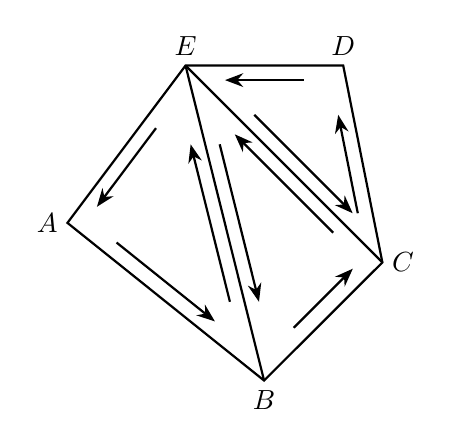
\begin{tikzpicture}
            \coordinate (A) at (0, 2.0025);
            \coordinate (B) at (2.4975, 0);
            \coordinate (C) at (4.0, 1.5);
            \coordinate (D) at (3.5025, 4.0);
            \coordinate (E) at (1.5, 4.0);

            \draw[thick] (A) -- (B) -- (C) -- (D) -- (E) -- cycle;
            \draw[thick] (B) -- (E);
            \draw[thick] (C) -- (E);

            \tikzhalflengtharrow{[xshift=-5.25pt]B}{[xshift=-5.25pt]E}
            \tikzhalflengtharrow{[xshift=5.25pt]E}{[xshift=5.25pt]B}
            \tikzhalflengtharrow{[yshift=-8.4pt]E}{[yshift=-8.4pt]A}
            \tikzhalflengtharrow{[yshift=8.4pt]B}{[yshift=8.4pt]C}
            \tikzhalflengtharrow{[yshift=7.125pt]A}{[yshift=7.125pt]B}
            \tikzhalflengtharrow{[yshift=-7.05pt]C}{[yshift=-7.05pt]E}
            \tikzhalflengtharrow{[xshift=7.05pt]E}{[xshift=7.05pt]C}
            \tikzhalflengtharrow{[yshift=-5.25pt]D}{[yshift=-5.25pt]E}
            \tikzhalflengtharrow{[xshift=-5.355pt]C}{[xshift=-5.355pt]D}

            \node[anchor=east] at (A) {\(A\)};
            \node[anchor=north] at (B) {\(B\)};
            \node[anchor=west] at (C) {\(C\)};
            \node[anchor=south] at (D) {\(D\)};
            \node[anchor=south] at (E) {\(E\)};

        \end{tikzpicture}
        \caption{A closed polygonal, chain internally triangulated.}\label{fig:cauchyintegraltheoremoversimplyconnectedset_closedpolygonalchaintriangulation}
    \end{figure}Since \(P\) is a closed polygonal chain, we can triangulate the interior. For example, consider \autoref{fig:cauchyintegraltheoremoversimplyconnectedset_closedpolygonalchaintriangulation}. Then,
    \begin{align*}
        \int_{ABCDE}f(z)\ddz & =\qty(\int_{\overrightarrow{AB}}+\int_{\overrightarrow{BC}}+\int_{\overrightarrow{CD}}+\int_{\overrightarrow{DE}}+\int_{\overrightarrow{EA}})f(z)\ddz \\
        & \quad+\qty(\int_{\overrightarrow{BE}}+\int_{\overrightarrow{EB}}+\int_{\overrightarrow{CE}}+\int_{\overrightarrow{EC}})f(z)\ddz                       \\
        & =\int_{\Delta{ABE}}f(z)\ddz+\int_{\Delta{BCE}}f(z)\ddz+\int_{\Delta{CDE}}f(z)\ddz.
    \end{align*} Thus, if the integral over every triangle in \(U\) vanishes, then equation~\eqref{eq:cauchyintegraltheoremoversimplyconnectedset_statement} follows. Consider a triangle in \(U\) with boundary \(\Delta\).
    \begin{figure}
        \centering
        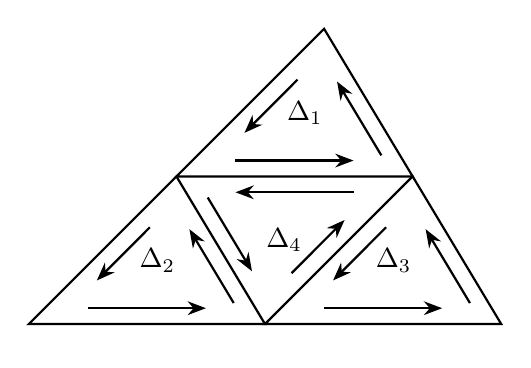
\begin{tikzpicture}
            \coordinate (A) at (0, 0);
            \coordinate (D) at (4.875, 1.875);
            \coordinate (F) at (1.875, 1.875);
            \coordinate (C) at (6, 0);
            \coordinate (B) at (3.75, 3.75);
            \coordinate (E) at (3, 0);

            \draw[thick] (A) -- (F) -- (E) -- cycle;
            \draw[thick] (B) -- (D) -- (F) -- cycle;
            \draw[thick] (C) -- (D) -- (E) -- cycle;

            \tikzhalflengtharrow{[yshift=-8.775pt]F}{[shift={(15pt, 6.15pt)}]A};
            \tikzhalflengtharrow{[yshift=-8.775pt]B}{[shift={(15pt, 6.15pt)}]F};
            \tikzhalflengtharrow{[yshift=-8.775pt]D}{[shift={(15pt, 6.15pt)}]E};
            \tikzhalflengtharrow{[yshift=8.775pt]E}{[shift={(-15pt, -6.15pt)}]D};

            \tikzhalflengtharrow{[shift={(-3.3075pt, -5.73pt)}]E}{[shift={(-3.3075pt, -5.73pt)}]F};
            \tikzhalflengtharrow{[shift={(-3.3075pt, -5.73pt)}]D}{[shift={(-3.3075pt, -5.73pt)}]B};
            \tikzhalflengtharrow{[shift={(-3.3075pt, -5.73pt)}]C}{[shift={(-3.3075pt, -5.73pt)}]D};
            \tikzhalflengtharrow{[shift={(3.3075pt, 5.73pt)}]F}{[shift={(3.3075pt, 5.73pt)}]E};

            \tikzhalflengtharrow{[yshift=5.73pt]A}{[yshift=5.73pt]E};
            \tikzhalflengtharrow{[yshift=5.73pt]E}{[yshift=5.73pt]C};
            \tikzhalflengtharrow{[yshift=5.73pt]F}{[yshift=5.73pt]D};
            \tikzhalflengtharrow{[yshift=-5.73pt]D}{[yshift=-5.73pt]F};

            \coordinate (AE) at ($(A)!0.5!(E)$);
            \coordinate (AF) at ($(A)!0.5!(F)$);
            \coordinate (FD) at ($(F)!0.5!(D)$);
            \coordinate (BF) at ($(B)!0.5!(F)$);
            \coordinate (EC) at ($(E)!0.5!(C)$);

            \path let
            \p1 = (FD),
            \p2 = (BF),
            \p3 = (AE),
            \p4 = (AF),
            \p5 = (EC)
            in
            node[shift={(3.75pt,-3.75pt)}] at (\x1, \y2) {\(\Delta_1\)}
            node[shift={(3.75pt,-3.75pt)}] at (\x3, \y4) {\(\Delta_2\)}
            node[shift={(3.75pt,-3.75pt)}] at (\x5, \y4) {\(\Delta_3\)}
            node[shift={(-3.75pt, 3.75pt)}] at (\x1, \y4) {\(\Delta_4\)};

        \end{tikzpicture}
        \caption{Quadrisection of the triangle bounded by \(\Delta\).}\label{fig:cauchyintegraltheoremoversimplyconnectedset_trianglequadrisection}
    \end{figure} Then define \(M\) to be \[M=\abs{\int_{\Delta}f(z)\ddz}.\]
    We can quadrisect the triangle bounded by \(\Delta\) into four triangles with boundaries \(\Delta_1,\Delta_2,\Delta_3,\Delta_4\) as in \autoref{fig:cauchyintegraltheoremoversimplyconnectedset_trianglequadrisection}. Then one of \(\Delta_1\), \(\Delta_2\), \(\Delta_3\), or \(\Delta_4\) (denote this to be \(\Delta^1\)) satisfy
    \[\abs{\int_{\Delta^1}f(z)\ddz}\geq\frac{M}{4},\]
    and recursively, choose
    \begin{equation}
        \abs{\int_{\Delta^2}f(z)\ddz}\geq\frac{M}{4^2},\ldots,\abs{\int_{\Delta^n}f(z)\ddz}\geq\frac{M}{4^n}. \label{eq:cauchyintegraltheoremoversimplyconnectedset_trianglelowerbound}
    \end{equation}
    Let \(L\) denote the perimeter of \(\Delta\). Then, the perimeters of \(\Delta^1, \Delta^2,\ldots\) respectively are \(\frac{L}{2},\frac{L}{2^2},\ldots\). As \(n\to\infty\), \(\Delta_n\) shrinks to a single point \(z_0\). Then, \(\forall n\in\mathbb{N}\), \(z_0\in\Delta^n\).

    By the definition of holomorphy, \(\forall\varepsilon>0\), \(\exists\delta>0\) such that \(\forall z\in D\paren{z_0,\delta}\), \[\abs{\frac{f\paren{z}-f\paren{z_0}}{z-z_0}-f'\paren{z_0}}<\varepsilon,\]\[\abs{f\paren{z}-f\paren{z_0}-f'\paren{z_0}\paren{z-z_0}}<\varepsilon\abs{z-z_0}.\] and \(\exists N\in\mathbb{N}\) such that \(\forall n\in \mathbb{N}_{>N}\), \(\Delta^n\subset D\paren{z_0,\delta}\). By \autoref{thm:cauchyintegraltheorem}, since the functions \(1\) and \(z\) are both entire, \[\int_{\Delta^n}\ddz=0,\quad\int_{\Delta^n}z\ddz=0.\] Then
    \begin{align*}
        \int_{\Delta^n}f(z)\ddz & =\int_{\Delta^n}f(z)\ddz-f\paren{z_0}\int_{\Delta^n}\ddz-f'\paren{z_0}\left(\int_{\Delta^n}z\ddz-z_0\int_{\Delta^n}\ddz\right) \\
        & =\int_{\Delta^n}\brackets{f(z)-f\paren{z_0}-f'\paren{z_0}\paren{z-z_0}}\ddz.
    \end{align*}
    Because the distance between any two points in the interior of a triangle is always less than its perimeter, using the triangle inequality for complex integrals, \[\int_{\Delta^n}\abs{f(z)}\abs{\ddz}\leq\varepsilon\int_{\Delta^n}\abs{z-z_0}\abs{\ddz}=\frac{\varepsilon L}{2^n}\int_{\Delta^n}\abs{\ddz}=\frac{\varepsilon L^2}{4^n}.\]
    Comparing the above equation with equation~\eqref{eq:cauchyintegraltheoremoversimplyconnectedset_trianglelowerbound}, \[\frac{M}{4^n}<\frac{\varepsilon L}{4^n},\quad M<\varepsilon L.\] Since \(\Delta\) is rectifiable, \(L\) is finite, and letting \(\varepsilon\to0\), we find that \(M\to0\). Then, for every triangle in \(U\), the integral vanishes, and equations~\eqref{eq:cauchyintegraltheoremoversimplyconnectedset_chainvanishingstatement} and~\eqref{eq:cauchyintegraltheoremoversimplyconnectedset_chaindefinition} follow.
\end{proof}
\begin{theorem}[Cauchy--Goursat]\label{thm:cauchygoursattheorem}
    Let \(U\subset\mathbb{C}\) be an open region bounded with boundary \(\partial U\). Let \(f:U\to\mathbb{C}\) be a holomorphic function continuous on \(\overline{U}\). Then, \[\oint_{\partial U}f(\zeta)\ddzeta=0.\]
\end{theorem}
\begin{proof}
    Since \(\partial U\cap U=\emptyset\) and \(f(z)\) is not necessarily holomorphic over \(\overline{U}\), we cannot directly apply \autoref{lemma:cauchyintegraltheoremoversimplyconnectedset}.
    \begin{figure}
        \centering
        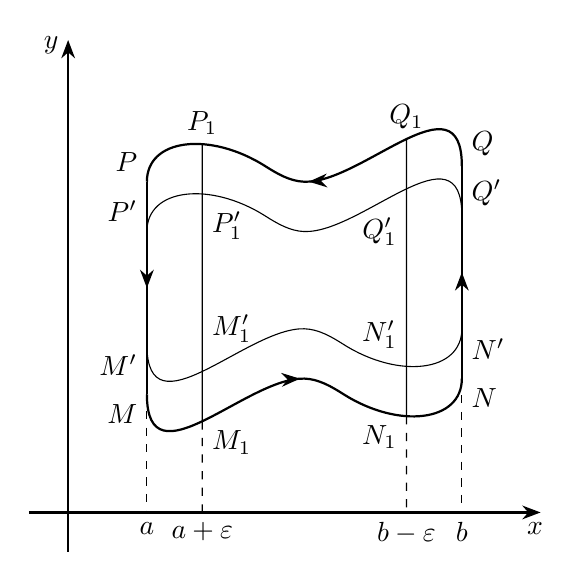
\begin{tikzpicture}[>=stealth,
                arrow style/.style={
                    postaction={decorate},
                    decoration={markings, mark=at position 0.5 with {\arrow[scale=1]{Stealth}}}
            }]
            \pgfmathsetmacro{\lengtheta}{18pt}
            \pgfmathsetmacro{\lengthepsilon}{20pt}
            \coordinate (M) at (1, 1.5);
            \coordinate (P) at (1, 4.2);
            \coordinate (Q) at (5, 4.4);
            \coordinate (N) at (5, 1.7);
            \coordinate (Mprime) at ([yshift=\lengtheta] M);
            \coordinate (Pprime) at ([yshift=-\lengtheta] P);
            \coordinate (Qprime) at ([yshift=-\lengtheta] Q);
            \coordinate (Nprime) at ([yshift=\lengtheta] N);
            \draw[-{Stealth}, thick] (-0.5, 0) -- (6, 0);
            \draw[-{Stealth}, thick] (0, -0.5) -- (0, 6);
            \draw[thick, arrow style] (P) -- (M);
            \draw[thick, arrow style, name path=curveQP] (Q) to[out angle=90, in angle=90, curve through = {([shift={(2, 0)}] P) ([shift={(1.5, 0.2)}] P)}] (P);
            \draw[thick, arrow style] (N) -- (Q);
            \draw[thick, arrow style, name path=curveMN] (M) to[out angle=270, in angle=270, curve through = {([shift={(-2, 0)}] N) ([shift={(-1.5, -0.2)}] N)}] (N);
            \path let \p1 = (P) in coordinate (P1x) at ({\x1 + \lengthepsilon}, 0);
            \path let \p1 = (Q) in coordinate (Q1x) at ({\x1 - \lengthepsilon}, 0);
            \path[name path=verticalleftmarker](P1x) -- (P1x |- 0, 6);
            \path[name path=verticalrightmarker](Q1x) -- (Q1x |- 0, 6);
            \path[name intersections={of=curveQP and verticalleftmarker, by=P1}];
            \path[name intersections={of=curveMN and verticalleftmarker, by=M1}];
            \draw[thin] (M1) -- (P1);
            \path[name intersections={of=curveQP and verticalrightmarker, by=Q1}];
            \path[name intersections={of=curveMN and verticalrightmarker, by=N1}];
            \draw[thin] (N1) -- (Q1);
            \draw[thin] (Mprime) to[out angle=270, in angle=270, curve through = {([shift={(-2, 0)}] Nprime) ([shift={(-1.5, -0.2)}] Nprime)}] (Nprime);
            \draw[thin] (Qprime) to[out angle=90, in angle=90, curve through = {([shift={(2, 0)}] Pprime) ([shift={(1.5, 0.2)}] Pprime)}] (Pprime);
            \draw[dashed] (M) -- (M |- 0, 0);
            \draw[dashed] (N) -- (N |- 0, 0);
            \draw[dashed] (M1) -- (P1x);
            \draw[dashed] (N1) -- (Q1x);
            \node[anchor=north east] at (M) {\(M\)};
            \node[anchor=south east] at (P) {\(P\)};
            \node[anchor=south west] at (Q) {\(Q\)};
            \node[anchor=north west] at (N) {\(N\)};
            \node[anchor=north east] at (Mprime) {\(M'\)};
            \node[anchor=south east] at (Pprime) {\(P'\)};
            \node[anchor=south west] at (Qprime) {\(Q'\)};
            \node[anchor=north west] at (Nprime) {\(N'\)};
            \node[anchor=north west] at (M1) {\(M_1\)};
            \node[anchor=south] at (P1) {\(P_1\)};
            \node[anchor=south] at (Q1) {\(Q_1\)};
            \node[anchor=north east] at (N1) {\(N_1\)};
            \node[anchor=south west] at ([yshift=\lengtheta+7pt] M1) {\(M'_1\)};
            \node[anchor=north west] at ([yshift=-\lengtheta-3pt] P1) {\(P'_1\)};
            \node[anchor=north east] at ([yshift=-\lengtheta-7pt] Q1) {\(Q'_1\)};
            \node[anchor=south east] at ([yshift=\lengtheta+3pt] N1) {\(N'_1\)};
            \node[anchor=north] at (M |- 0, 0) {\(a\)};
            \node[anchor=north] at (N |- 0, 0) {\(b\)};
            \node[anchor=north] at (P1x |- 0, 0) {\(a+\varepsilon\)};
            \node[anchor=north] at (Q1x |- 0, 0) {\(b-\varepsilon\)};
            \node[anchor=north, xshift=-2pt] at (6, 0) {\(x\)};
            \node[anchor=east, yshift=-2pt] at (0, 6) {\(y\)};
        \end{tikzpicture}
        \caption{A simplified region containing two vertical lines and two continuous, rectifiable curves.}
        \label{fig:cauchygoursattheorem_simplifiedregion}
    \end{figure}

    First assume \(U\) has the shape of \(MNQP\) in \autoref{fig:cauchygoursattheorem_simplifiedregion}. That is, \(U\) consists of \(x=a\), \(x=b\) for \(a<b\), and two rectifiable \(C^0\) curves \(\overrightarrow{MN}:y=\varphi(x)\) and \(\overrightarrow{QP}:\psi(x)\) such that \(\varphi(x)<\psi(x)\), \(\forall a\le x\le b\).

    For some \(\varepsilon>0\), \(\eta>0\), construct a new curve \(M_1'N_1'Q_1'P_1'\in U\) to be the boundary of the region bounded by \(P_1M_1:x=a+\varepsilon\), \(N_1Q_1:b-\varepsilon\), \(M'N':\varphi(x)+\eta\), and \(Q'P': \psi(x)-\eta\) such that \(M_1'N_1'Q_1'P_1'\) remains simple. By \autoref{lemma:cauchyintegraltheoremoversimplyconnectedset}, \[\oint_{M_1'N_1'Q_1'P_1'}f(z)\ddz=0.\]
    By \autoref{thm:heinecantor}, \(f(z)\) is uniformly continuous over \(\overline{U}\), and therefore \(\forall\varepsilon'>0\), we can choose \(\eta>0\) so that \(\forall z\in\overrightarrow{M_1'N_1'}\), \(\abs{f\paren{z}-f\paren{z-\eta}}<\varepsilon'\) is satisfied. Letting \(\eta\to0\) (with \(\varepsilon'\to0\)) and fixing \(\varepsilon>0\), we get that
    \begin{align*}
        \abs{\int_{\overrightarrow{M_1'N_1'}}f(z)\ddz-\int_{\overrightarrow{M_1N_1}}f(z)\ddz} & \leq\int_{\overrightarrow{M_1'N_1'}}\abs{f(z)-f\paren{z-\eta}}\abs{\ddz} \\
        & <\varepsilon'\int_{\overrightarrow{M_1'N_1'}}\abs{dz}\to0,
    \end{align*}
    and consequently,
    \begin{equation}
        \int_{\overrightarrow{M_1'N_1'}}f(z)\ddz\to \int_{\overrightarrow{M_1N_1}}f(z)\ddz.\label{eq:cauchygoursattheorem_innerinnerhorizontaltoouterinnerhorizontal1}
    \end{equation}
    Under the same limit, we get
    \begin{equation}
        \int_{\overrightarrow{Q_1'P_1'}}f(z)\ddz\to \int_{\overrightarrow{Q_1P_1}}f(z)\ddz.\label{eq:cauchygoursattheorem_innerinnerhorizontaltoouterinnerhorizontal2}
    \end{equation} By the continuity of \(f(z)\) over a compact set,
    \begin{equation}
        \int_{\overrightarrow{P_1'M_1'}}f(z)\ddz\to \int_{\overrightarrow{P_1M_1}}f(z)\ddz,\quad\int_{\overrightarrow{N_1'Q_1'}}f(z)\ddz\to \int_{\overrightarrow{N_1Q_1}}f(z)\ddz.\label{eq:cauchygoursattheorem_innerinnerverticaltoouterinnervertical}
    \end{equation}
    Then letting \(\varepsilon\to0\), for the same reason as equation~\eqref{eq:cauchygoursattheorem_innerinnerverticaltoouterinnervertical}, equations~\eqref{eq:cauchygoursattheorem_innerinnerhorizontaltoouterinnerhorizontal1} and~\eqref{eq:cauchygoursattheorem_innerinnerhorizontaltoouterinnerhorizontal2} yield \[\int_{\overrightarrow{M_1N_1}}f(z)\ddz\to \int_{\overrightarrow{MN}}f(z)\ddz,\quad\int_{\overrightarrow{Q_1P_1}}f(z)\ddz\to \int_{\overrightarrow{QP}}f(z)\ddz.\]
    We are left to show the subsequent limits of the results from equation~\eqref{eq:cauchygoursattheorem_innerinnerverticaltoouterinnervertical}. For the left integral, let \(y_{\varphi}=\max\paren{\varphi(a),\varphi\paren{a+\varepsilon}}\) and \(y_{\psi}=\max\paren{\psi(a),\psi\paren{a+\varepsilon}}\).

    Then, \[\int_{\overrightarrow{PM}}f(z)\ddz=\ii\int_{\psi(a)}^{\varphi(a)}f\paren{a+\ii y}\ddy=\ii\paren{\int_{\psi(a)}^{y_\varphi}+\int_{y_\varphi}^{y_\psi}+\int_{y_\psi}^{\varphi(a)}}f(a+\ii y)\ddy.\]
    Similarly, \[\int_{\overrightarrow{P_1M_1}}f(z)\ddz=\ii\paren{\int_{\psi(a+\varepsilon)}^{y_\varphi}+\int_{y_\varphi}^{y_\psi}+\int_{y_\psi}^{\varphi(a+\varepsilon)}}f(a+\varepsilon+\ii y)\ddy.\]
    The difference \(\paren{\int_{\overrightarrow{PM}}-\int_{\overrightarrow{P_1M_1}}}f(z)\ddz\) between the two is then equal to
    \begin{gather*}
        \ii\int_{y_{\varphi}}^{y_{\psi}}\paren{f\paren{a+\ii y}-f\paren{a+\varepsilon+\ii y}}\ddz\\
        {}+{\ii\paren{\int_{\psi(a)}^{y_\varphi}+\int_{y_\psi}^{\varphi(a)}}f(a+\ii y)-\ii\paren{\int_{\psi(a+\varepsilon)}^{y_\varphi}z+\int_{y_\psi}^{\varphi\paren{a+\varepsilon}}}f(a+\varepsilon+\ii y)}.
    \end{gather*}
    The first term vanishes by uniform continuity (through the same argument used for \(M_1'N_1'\to M_1N_1\)) and the remaining four integrals all equal 0 as they are all integrable on a degenerating interval (as \(\varepsilon\to0\), \(y_\varphi\to\varphi(a)\) and \(y_\psi\to\psi(a)\) because \(\varphi, \psi\in C^0\)). Therefore, \[\int_{\overrightarrow{P_1M_1}}f(z)\ddz\to\int_{\overrightarrow{PM}}f(z)\ddz,\]
    and through similar logic, \[\int_{\overrightarrow{N_1Q_1}}f(z)\ddz\to\int_{\overrightarrow{NQ}}f(z)\ddz.\] Therefore, \[\oint_{MNQP}f(z)\ddz=0.\]
    Any open region \(U\subset\mathbb{C}\) with a simple closed boundary can be broken up into smaller regions with the same form as \(MNQP\) with finitely many auxiliary lines. Then the conclusion follows.
\end{proof}
\begin{remark}
    The theorem is also valid for any multiply connected region (and its boundary will consist of multiple curves) as a multiply connected region is equal to the union of several simply connected regions with vertical auxiliary lines between.

    Additionally, if \(U\subset\mathbb{C}\) is simply connected and \(f\) is holomorphic on \(U\), then for any two points \(z,z_0\in U\), the integral \[\int_{z_0}^z f(\zeta)\ddzeta\] is well-defined and independent of the path taken from \(z_0\) to \(z\). In this sense, a holomorphic function behaves analogously to a potential field.
\end{remark}
\begin{theorem}[Cauchy--Goursat]\label{thm:cauchygoursatformula}
    Let \(U\subset\mathbb{C}\) be an open region bounded with a simple closed boundary \(\partial U \), and let \(f:U\to\mathbb{C}\) be a holomorphic function continuous on \(\overline{U}\). Then for all \(z\in U\),
    \begin{equation}
        f(z)=\frac{1}{2\piup\ii}\oint_{\partial U}\frac{f(\zeta)}{\zeta-z}\ddzeta.\label{eq:cauchygoursatformula}
    \end{equation}
\end{theorem}
\begin{proof}
    By the Cauchy--Goursat Theorem (\autoref{thm:cauchygoursattheorem}), \[\int_{\partial\paren{U\setminus D(z,\varepsilon)}}\frac{f(\zeta)}{\zeta-z}\ddzeta=\oint_{\partial U}\frac{f(\zeta)}{\zeta-z}\ddzeta-\oint_{\partial D(z,\varepsilon)}\frac{f(\zeta)}{\zeta-z}\ddzeta=0.\]
    From rearrangement, \[\oint_{\partial U}\frac{f(\zeta)}{\zeta-z}\ddzeta=2\piup \ii f(z)+\ii\int_0^{2\piup}\paren{f\paren{z+\varepsilon \ee^{\ii t}}-f(z)}\dd{t}.\]
    Since \(f\in C^0(\partial D(z,\varepsilon))\), as \(\varepsilon\to0\),
    \begin{align*}
        \abs{\int_0^{2\piup}\paren{f\paren{z+\varepsilon \ee^{\ii t}}-f(z)}\dd{t}} & \leq\int_0^{2\piup}\abs{f\paren{z+\varepsilon \ee^{\ii t}}-f(z)}\dd{t} \\
        & \leq2\piup\max\abs{f\paren{z+\varepsilon \ee^{\ii t}}-f(z)}\to0.
    \end{align*}
    By rearrangement, \[f(z)=\frac{1}{2\piup\ii}\oint_{\partial U}\frac{f(\zeta)}{\zeta-z}\ddzeta.\]
\end{proof}
\begin{remark}
    In the proof of \autoref{thm:pompeiu}, we used Lipschitz continuity for a smooth function, which was a stronger condition than necessary. The true necessity of smoothness was to be able to apply Green's Theorem (\autoref{thm:complexgreen}).
\end{remark}
This profound theorem is extremely important and helpful in complex integration and essential in the evaluation of integrals, as demonstrated below.
\begin{example}\label{ex:cauchygoursatformulazeroofunity}
    Evaluate the integral \(\int_{\partial D(0,2)}\frac{\ddz}{z^n-1}\), where \(n\in\mathbb{N}_{\geq 2}\).
\end{example}
\begin{proof}
    Since \(z^n-1=\prod_{k=0}^{n-1}\qty(z-\omega^k_n)\), where \(\omega^k_n=\ee^{\ii\piup\frac{k}{n}}\), the integrand has singularities at every \(n\)th zero of unity. Then the integral is equal to:
    \begin{equation}
        \int_{\partial D(0,2)}\frac{\ddz}{\prod_{j=0}^{n-1}\qty(z-\omega_j)}=\int_{\partial D(0,2)}\sum_{j=0}^{n-1}\frac{c_j}{z-\omega_j}\ddz,\label{eq:cauchygoursatformulazerosofunity}
    \end{equation}
    where \(\cbraces{c_j}\) are the coefficients of the partial fraction decomposition. By the Cauchy--Goursat Formula (\autoref{thm:cauchygoursatformula}), equation~\eqref{eq:cauchygoursatformulazerosofunity} becomes: \[\sum_{k=0}^{n-1}\int_{\partial D(0,2)}\frac{c_k}{z-\omega_k}\ddz=2\piup\ii\sum_{k=0}^{n-1}c_k.\]
    Observe that \(\sum_{k=0}^{n-1} c_k=\lim_{z\to\infty}\sum_{k=0}^{n-1}\frac{zc_k}{z-\omega_k}=\lim_{z\to\infty}\frac{z}{z^n-1}=0\) since \(n\geq2\).
    Therefore, \[\int_{\partial D(0,2)}\frac{\ddz}{z^n-1}=0.\]
\end{proof}
We have also already seen the utility of parameterization via a polar transformation. Many useful identities in classical calculus can also be derived from concepts in its generalization:
\begin{example}
    Prove that \(\forall n\in\mathbb{N}\), \[\int_{0}^{2\piup}\cos^{2n}\theta\dd{\theta}=2\piup\prod_{k=1}^n\frac{2k-1}{2k}.\]
\end{example}
\begin{proof}
    Consider the integral \[\int_{\partial\mathbb{D}}\qty(z+\frac{1}{z})^{2n}\frac{\ddz}{z}.\]
    Letting \(z=\ee^{\ii\theta}\), we get \(\int_{\partial\mathbb{D}}\qty(\ee^{\ii\theta}+\ee^{-\ii\theta})^{2n}\ee^{-\ii\theta}\ddz=2^{2n}\ii\int_0^{2\piup}\cos^{2n}\theta\dd{\theta}\). Alternatively, we can expand the integrand and get \[\int_{\partial\mathbb{D}}\sum_{k=0}^{2n}\binom{2n}{k}z^{2k-2n}\frac{\ddz}{z}=\sum_{k=0}^{2n}\int_{\partial\mathbb{D}}\binom{2n}{k}z^{2k-2n-1}\ddz.\]
    When \(2k-2n-1\ge0\), the integrand is holomorphic. The integral is then equal to \[\binom{2n}{0}\int_{\partial\mathbb{D}}z^{-2n-1}\ddz+\binom{2n}{1}\int_{\partial\mathbb{D}}z^{-2n+1}\ddz+\cdots+\binom{2n}{n}\int_{\partial\mathbb{D}}\frac{\ddz}{z}=2\piup\ii\binom{2n}{n},\]
    since all of the higher order terms vanish:
    \[\int_{\partial\mathbb{D}}z^{2k-2n-1}\ddz=\int_0^{2\piup} \ee^{\ii\theta\qty(2k-2n-1)}\ii\ee^{\ii\theta}\dd{\theta}=\ii\int_0^{2\piup}\ee^{2\ii\theta(k-n)}\dd{\theta}=
        \begin{cases}
            0       & k< n \\
            2\piup\ii & k=n
    \end{cases}.\]
    Therefore, \[2^{2n}\ii\int_0^{2\piup}\cos^{2n}\theta\dd{\theta}=2\piup\ii\binom{2n}{n}\Longleftrightarrow\int_0^{2\piup}\cos^{2n}\theta\dd{\theta}=\frac{2\piup\qty(2n)!}{2^{2n}\qty(n!)^2}=\frac{2\piup\prod_{k=1}^{2n}k}{\prod_{k=1}^{n}{\qty(2k)}^2}.\]
    From simple cancellation, we get \[2\piup\frac{\prod_{k=1}^{n}\qty(2k-1)}{\prod_{k=1}^n\qty(2k)}=2\piup\prod_{k=1}^n\frac{2k-1}{2k},\]
    as expected.
\end{proof}
\begin{example}[Cauchy--Goursat Formula on the Exterior]\label{ex:cauchygoursatformulaexterior}
    Let \(\gamma\subset\mathbb{C}\) be a simple closed curve, and suppose that \(f:\mathrm{ext}(\gamma)\to\mathbb{C}\) is holomorphic and continuous on \(\overline{\mathrm{ext}(\gamma)}=\mathbb{C}\setminus\mathrm{int}(\gamma)\), where \(\mathrm{int}\) and \(\mathrm{ext}\) respectively denote the interior and exterior as in \autoref{thm:jordancurve}.
    \begin{enumerate}
        \item If \(f\) has a removable singularity at \(\infty\), or if \(w=\lim_{z\to\infty} f(z)\) exists and is finite, then \(\forall z\in\mathbb{C}\setminus\gamma\), \[\frac{1}{2\piup\ii}\int_\gamma\frac{f(\zeta)}{\zeta-z}\ddzeta=
                \begin{cases}
                    w      & z\in\mathrm{int}(\gamma) \\
                    w-f(z) & z\in\mathrm{ext}(\gamma)
            \end{cases}.\]
        \item If \(\gamma\) encloses the origin, then \(\forall z\in\mathbb{C}\setminus\gamma\), then
            \begin{equation}
                \frac{1}{2\piup\ii}\int_\gamma\frac{zf(\zeta)}{z\zeta-\zeta^2}\ddzeta=
                \begin{cases}
                    0    & z\in\mathrm{int}(\gamma)                                                       \\
                    f(z) & z\in\mathrm{ext}(\gamma)\label{eq:cauchygoursatformulaexteriorpart2_statement}
                \end{cases}.
            \end{equation}
    \end{enumerate}
\end{example}
\begin{proof}
    \begin{enumerate}
        \item By the compactness of \(\gamma\), it can be completely contained within a sufficiently large disk centered at the origin (\(\gamma\subset D(0,R)\)). Then by applying \autoref{thm:cauchygoursatformula} or \autoref{thm:cauchygoursattheorem} on the set \(D(0,R)\cap\mathrm{ext}(\gamma)=D(0,R)\setminus\overline{\mathrm{int}(\gamma)}\), we get that \[\frac{1}{2\piup\ii}\int_{\partial D(0,R)}\frac{f(\zeta)}{\zeta-z}\ddzeta=\frac{1}{2\piup\ii}\int_\gamma\frac{f(\zeta)}{\zeta-z}\ddzeta+
                \begin{cases}
                    0    & z\in\mathrm{int}(\gamma)            \\
                    f(z) & z\in D(0,R)\cap\mathrm{ext}(\gamma)
            \end{cases}.\]
            By letting \(R\to\infty\) and letting \(\zeta=R\ee^{\ii\theta}\), we get that \[\frac{1}{2\piup\ii}\int_\gamma\frac{f(\zeta)}{\zeta-z}\ddzeta=\frac{1}{2\piup}\lim_{R\to\infty}\int_0^{2\piup}\frac{f\qty(R\ee^{\ii\theta})}{1-\frac{z}{R\ee^{\ii\theta}}}\dd{\theta}-
                \begin{cases}
                    0    & z\in\mathrm{int}(\gamma) \\
                    f(z) & z\in\mathrm{ext}(\gamma)
            \end{cases}.\]
            By the continuity of \(f\) on \(\partial D(0,R)\), it attains its maximum \(M\). For sufficiently large \(R\), \(\abs{1-\frac{z}{R\ee^{\ii\theta}}}\) attains a positive minimum. Then the integrand is uniformly bounded with respect to \(R\) under \(\theta\), and we can commute the limit with the integral. Hence,
            \begin{align*}
                \frac{1}{2\piup\ii}\int_\gamma\frac{f(\zeta)}{\zeta-z}\ddzeta & =\frac{1}{2\piup}\int_0^{2\piup}\frac{w}{1-\lim_{R\to\infty}\frac{z}{R\ee^{\ii\theta}}}\dd{\theta}-
                \begin{cases}
                    0    & z\in\mathrm{int}(\gamma) \\
                    f(z) & z\in\mathrm{ext}(\gamma)
                \end{cases}                                                                                                                               \\   & =
                \begin{cases}
                    w      & z\in\mathrm{int}(\gamma) \\
                    w-f(z) & z\in\mathrm{ext}(\gamma)
                \end{cases},
            \end{align*} as expected.
        \item Under the partial fraction decomposition of equation~\eqref{eq:cauchygoursatformulaexteriorpart2_statement}, we get that
            \begin{align}
                I & =\int_\gamma\frac{zf(\zeta)}{z\zeta-\zeta^2}\ddzeta=\int_\gamma\qty(\frac{f(\zeta)}{\zeta}-\frac{f(\zeta)}{\zeta-z})\ddzeta\nonumber \\
                & =\int_0^{2\piup}\qty(f\qty(R\ee^{\ii\theta})-\frac{f\qty(R\ee^{\ii\theta})}{1-\frac{z}{R\ee^{\ii\theta}}})\dd{\theta}+
                \begin{cases}
                    0            & z\in\mathrm{int}(\gamma)            \\
                    2\piup\ii f(z) & z\in\mathrm{ext}(\gamma)\cap D(0,R)
                \end{cases},\label{eq:cauchygoursatformulaexteriorpart2_prelimitintegral}
            \end{align} when \(\gamma\subset D(0,R)\).
            We will analyze the first integral as \(R\to\infty\). By the triangle and reverse triangle inequalities,
            \begin{align*}
                \qty|\int_0^{2\piup}\qty(f\qty(R\ee^{\ii\theta})-\frac{f\qty(R\ee^{\ii\theta})}{1-\frac{z}{R\ee^{\ii\theta}}})\dd{\theta}| & \leq\int_0^{2\piup}\qty|\frac{z}{R\ee^{\ii\theta}-z}|\dd{\theta}           \\
                & \leq\int_0^{2\piup}\frac{|z|}{R-|z|}\dd{\theta}=\frac{2\piup|z|}{R-|z|}\to0.
            \end{align*}
    \end{enumerate}
    By plugging the result into equation~\eqref{eq:cauchygoursatformulaexteriorpart2_prelimitintegral}, and letting \(R\to\infty\), we get that \[\frac{1}{2\piup\ii}\int_\gamma\frac{zf(\zeta)}{z\zeta-\zeta^2}\ddzeta=
        \begin{cases}
            0    & z\in\mathrm{int}(\gamma) \\
            f(z) & z\in\mathrm{ext}(\gamma)
    \end{cases}.\]
\end{proof}
\subsection{Analyticity and Holomorphy}\label{sec:analyticityandholomorphy}
The Cauchy--Goursat Formula (\autoref{thm:cauchygoursatformula}) can also be generalized into a result that equates complex integration and differentiation:
\begin{theorem}[Cauchy--Goursat Differentiation Formula]\label{thm:cauchydifferentiationformula}
    Let \(U\subset\mathbb{C}\) be an open region bounded by a simple closed boundary \(\partial U\), and let \(f:U\to\mathbb{C}\) be holomorphic and continuous over \(\overline{U}\). Then \(\forall z\in U\), \(\forall n\in\mathbb{N}\), \(f^{(n)}(z)\) exists, and
    \begin{equation}
        f^{(n)}(z)=\frac{n!}{2\piup\ii}\oint_{\partial U}\frac{f(\zeta)}{\paren{\zeta-z}^{n+1}}\ddzeta.\label{eq:cauchydifferentiationformula_statement}
    \end{equation}
    Additionally, since \(U\) is open, \(\forall z_0\in U\), \(\forall r>0\) such that the closed disk \(\overline{D\paren{z_0,r}}\subset U\), \(f\) has the uniformly and absolutely convergent Taylor expansion
    \begin{equation}
        f(z)=\sum_{j=0}^\infty a_j\paren{z-z_0}^j,\label{eq:cauchydifferentiationformula_taylorseries}
    \end{equation}
    where
    \begin{equation}
        a_j=\frac{1}{2\piup\ii}\oint_{\partial U}\frac{f(\zeta)}{\paren{\zeta-z}^{j+1}}\ddzeta\label{eq:cauchydifferentiationformula_taylorseriescoefficients}
    \end{equation} on \(\overline{D\paren{z_0,r}}\).
\end{theorem}
\begin{proof}
    \(\forall z_0\in U\), \(\forall z\in D\paren{z_0,r}\subset U\), by \autoref{thm:cauchygoursatformula}, \[f(z)-f\paren{z_0}=\frac{1}{2\piup\ii}\oint_{\partial U}\paren{\frac{f(\zeta)}{\zeta-z}-\frac{f(\zeta)}{\zeta-z_0}}\ddzeta=\frac{z-z_0}{2\piup\ii}\oint_{\partial U}\frac{f(\zeta)\ddzeta}{\paren{\zeta-z}\paren{\zeta-z_0}},\]
    and dividing by \(z-z_0\), the above is equal to \[\frac{f(z)-f\paren{z_0}}{z-z_0}=\frac{1}{2\piup\ii}\oint_{\partial U}\frac{f(\zeta)\ddzeta}{\paren{\zeta-z}\paren{\zeta-z_0}}.\]
    Since
    \begin{align}
        \frac{f(z)-f\paren{z_0}}{z-z_0}-\frac{1}{2\piup\ii}\oint_{\partial U}\frac{f(\zeta)\ddzeta}{\paren{\zeta-z_0}^2} & =\frac{1}{2\piup\ii}\oint_{\partial U}\frac{f\paren{\zeta}}{\zeta-z_0}\paren{\frac{1}{\zeta-z}-\frac{1}{\zeta-z_0}}\ddzeta\nonumber                                      \\
        & =\frac{z-z_0}{2\piup\ii}\oint_{\partial U}\frac{f(\zeta)}{(\zeta-z)\paren{\zeta-z_0}^2}\ddzeta.\label{eq:cauchydifferentiationformula_differenceoffirstorderdifferences}
    \end{align}
    Let \(d\) be the distance from \(z_0\) to \(\partial U\), and it follows that \(0<r<d\). Then, since \(\abs{z-z_0}<r\) and \(\abs{\zeta-z_0}\geq d\), \(\abs{\zeta-z}\geq d-r\). Then the absolute value of the integrand of equation~\eqref{eq:cauchydifferentiationformula_differenceoffirstorderdifferences} is bounded above by \(\frac{M}{d^2(d-r)}\), where \(M\) is the maximum of \(f(\zeta)\), which exists by \autoref{thm:continuousfunctionboundedoncompact}. Then, \[\abs{\frac{z-z_0}{2\piup\ii}\oint_{\partial U}\frac{f(\zeta)}{(\zeta-z)\paren{\zeta-z_0}^2}\ddzeta}\leq\frac{\abs{z-z_0}}{2\piup}\frac{M}{d^2(d-r)}\oint_{\partial U}\abs{\ddzeta}.\] As \(z\to z_0\), the difference vanishes, and therefore, \[f'\paren{z_0}=\frac{1}{2\piup\ii}\oint_{\partial U}\frac{f(\zeta)}{\paren{\zeta-z_0}^2}\ddzeta.\]
    Now inductively assume that equation~\eqref{eq:cauchydifferentiationformula_statement} is true for a given \(n=k\in\mathbb{N}\), or \[f^{(k)}(z)=\frac{k!}{2\piup\ii}\oint_{\partial U}\frac{f(\zeta)}{\paren{\zeta-z}^{k+1}}\ddzeta.\]
    Notice the expansion of the kernel, convergent since \(\abs{z-z_0}<\abs{\zeta-z_0}\):
    \begin{equation}
        \frac{1}{\zeta-z}=\frac{1}{\zeta-z_0}\cdot\frac{\zeta-z_0}{\zeta-z}=\frac{1}{\zeta-z_0}\cdot\frac{1}{1-\frac{z-z_0}{\zeta-z_0}}=\frac{1}{\zeta-z_0}\sum_{j=0}^{\infty}\paren{\frac{z-z_0}{\zeta-z_0}}^j.\label{eq:cauchydifferentiationformula_kernelexpansion}
    \end{equation}
    Then,
    \begin{align*}
        f^{(k)}(z) & =\frac{k!}{2\piup\ii}\oint_{\partial U}\frac{f(\zeta)}{(\zeta-z)^{k+1}}\ddzeta                                                                           \\
        & =\frac{k!}{2\piup\ii}\oint_{\partial U}\frac{f(\zeta)}{\paren{\zeta-z_0}^{k+1}}\paren{\sum_{j=0}^{\infty}\paren{\frac{z-z_0}{\zeta-z_0}}^j}^{k+1}\ddzeta \\
        & =f^{(k)}\paren{z_0}+\frac{(k+1)!\paren{z-z_0}}{2\piup\ii}\oint_{\partial U}\frac{f(\zeta)}{\paren{\zeta-z_0}^{k+2}}\ddzeta                               \\
        & \quad+\order{\abs{z-z_0}^2},
    \end{align*}
    where the remainder terms \(\order{\abs{z-z_0}^2}\) resemble
    \[\paren{z-z_0}^2\frac{k!}{2\piup\ii}\brackets{k+1+\binom{k+1}{2}}\oint_{\partial U}\frac{f(\zeta)}{\paren{\zeta-z_0}^{k+3}}\ddzeta+\mathcal{O}_{z\to z_0}\paren{\abs{z-z_0}^3}.\]
    The difference quotient is equal to \[\frac{f^{(k)}(z)-f^{(k)}\paren{z_0}}{z-z_0}=\frac{(k+1)!}{2\piup\ii}\oint_{\partial U}\frac{f(\zeta)}{\paren{\zeta-z_0}^{k+2}}\ddzeta+\mathcal{O}_{z\to z_0}\abs{z-z_0}.\] As \(z\to z_0\), the remainder terms vanish, and \[f^{(k+1)}\paren{z_0}=\frac{(k+1)!}{2\piup\ii}\oint_{\partial U}\frac{f(\zeta)}{\paren{\zeta-z_0}^{k+2}}\ddzeta.\]
    By induction, equation~\eqref{eq:cauchydifferentiationformula_statement} is valid. By substituting equation~\eqref{eq:cauchydifferentiationformula_kernelexpansion} into \eqref{eq:cauchygoursatformula}, we obtain \[f(z)=\frac{1}{2\piup\ii}\oint_{\partial U}\frac{f(\zeta)}{\zeta-z_0}\sum_{j=0}^{\infty}\paren{\frac{z-z_0}{\zeta-z_0}}^j\ddzeta=\frac{1}{2\piup\ii}\oint_{\partial U}\sum_{j=0}^{\infty}\paren{z-z_0}^j\frac{f(\zeta)\ddzeta}{\paren{\zeta-z_0}^{j+1}}.\]
    Because \(f(\zeta)\) is continuous over \(\partial U\), it is bounded by a constant \(M\). Additionally, since \(\abs{z-z_0}<\abs{\zeta-z_0}\), the sum is termwise bounded by the convergent series \[\sum_{j=0}^\infty\frac{Mr^j}{\inf_{\xi\in\partial U}\abs{\xi-z_0}^{j+1}}.\]
    By the Weierstrass \(M\)--Test (\autoref{thm:weierstrassmtest}), the series uniformly converges, and we can justify
    \begin{gather*}
        \frac{1}{2\piup\ii}\oint_{\partial U}\sum_{j=0}^{\infty}\paren{z-z_0}^j\frac{f(\zeta)}{\paren{\zeta-z_0}^{j+1}}\ddzeta=\frac{1}{2\piup\ii}\sum_{j=0}^{\infty}\oint_{\partial U}\paren{z-z_0}^j\frac{f(\zeta)}{\paren{\zeta-z_0}^{j+1}}\ddzeta\\=\sum_{j=0}^\infty a_j\paren{z-z_0}^j,
    \end{gather*}
    which verifies equations~\eqref{eq:cauchydifferentiationformula_taylorseries} and~\eqref{eq:cauchydifferentiationformula_taylorseriescoefficients}.
\end{proof}
\begin{remark}
    By induction, we have shown that assuming the existence of the first order derivative of a holomorphic function \(f\), the \(n\)th order derivative of \(f\) exists \(\forall n\in\mathbb{N}\) and is holomorphic over the same region as \(f^{(n-1)}\). Furthermore, if \(f\) is holomorphic, then \(\forall z\in U\), there exists an open disk enclosing \(z\) such that \(f\) has a convergent Taylor series expansion. This property is known as \textit{analyticity}, and \autoref{thm:cauchydifferentiationformula} tells us that all holomorphic functions are analytic. Analytic functions can be expanded into power series, which are termwise differentiable, and therefore complex differentiable. Thus, analyticity and holomorphy are logically equivalent, which is a fundamental difference between real and complex functions.
\end{remark}
The differentiation formula above can be thought of as a generalization of \autoref{thm:cauchygoursatformula}, and provides similar utility in the evaluation of integrals:
\begin{example}\label{ex:legendrepolynomialintegralformula}
    A \textit{Legendre polynomial} is a polynomial whose explicit equation is given by
    \begin{equation}
        P_n(z)=\frac{1}{2^n n!}\dv[n]{z}(\qty(z^2-1)^n).\label{eq:legendrepolynomialintegralformula_rodriguesformula}
    \end{equation}
    Prove the integral form \[P_n(z)=\frac{1}{2\piup\ii}\oint_\gamma\frac{\qty(\zeta^2-1)^n}{2^n{(\zeta-z)}^{n+1}}\ddzeta,\] where \(\gamma\) is a simple closed curve enclosing \(z\).
\end{example}
\begin{proof}
    By applying the Cauchy--Goursat Differentiation Formula (\autoref{thm:cauchydifferentiationformula}) on equation~\eqref{eq:legendrepolynomialintegralformula_rodriguesformula}, we get that \[P_n(z)=\frac{1}{2^{n+1}\piup \ii}\int_{\gamma}\frac{\qty(\zeta^2-1)^n}{{(\zeta-z)}^{n+1}}\ddzeta,\] as desired.
\end{proof}
\begin{theorem}[Cauchy's Estimate]\label{thm:cauchysestimate}
    For a function \(f:U\to\mathbb{C}\) holomorphic over \(U\subseteq\mathbb{C}\) and \(\forall z_0\in U\) and \(\forall R>0\) such that \(\overline{D\paren{z_0,R}}\subseteq{U}\), \(\forall n\in\mathbb{N}\), \[\abs{f^{(n)}\paren{z_0}}\leq\frac{n!M}{R^n},\]
    where \[M=\max_{z\in\overline{D\paren{z_0,R}}}\abs{f(z)}.\]
\end{theorem}
\begin{proof}
    By the Cauchy--Goursat Differentiation Formula (\autoref{thm:cauchydifferentiationformula}), \(\forall n\in\mathbb{N}\), \[f^{(n)}\paren{z_0}=\frac{n!}{2\piup\ii}\oint_{\partial D\paren{z_0,R}}\frac{f(\zeta)}{\paren{\zeta-z_0}^{n+1}}\ddzeta.\]
    Because \(f(z)\) is continuous over the boundary \(\partial D\paren{z_0,R}\), it is bounded by \(M\). Thus,
    \[\abs{f^{(n)}\paren{z_0}}\leq\frac{n!}{2\piup}\int_0^{2\piup}\frac{M}{\paren{\ee^{\ii\theta}R}^{n+1}}\ee^{\ii\theta}R\dd{\theta}=\frac{n!M}{R^n},\] as desired.
\end{proof}
\autoref{thm:nthderivativeboundedl1norm} will profoundly generalize this statement significantly. The relationship between the derivatives of a holomorphic function and the function itself is an important property of holomorphic functions.
\begin{example}
    Let \(f\) be entire and \(\forall z\in\mathbb{C}\), \(|f(z)|\leq M\ee^{|z|}\). Prove that \(\forall n\in\mathbb{N}\), \(|f(0)|\leq M\) and \[\abs{f^{(n)}(0)}\leq Mn!\qty(\frac{\ee}{n})^n.\]
\end{example}
\begin{proof}
    \(|f(0)|\leq M\) is obviously true by letting \(z=0\). Then \(\forall R>0\), by Cauchy's Estimate (\autoref{thm:cauchysestimate}), \[\abs{f^{(n)}(0)}\leq Mn!\frac{\ee^{R}}{R^n}.\]
    By letting \(R=n\), the conclusion follows. In fact, this is the tightest possible inequality. Consider \(\varphi(R)=Mn!\frac{\ee^R}{R^n}\) to be a function of \(R\). It attains its minimum as its derivative vanishes:
    \[\varphi'(R)=Mn!\frac{\ee^RR^n-n\ee^RR^{n-1}}{R^{2n}}=0\Longleftrightarrow R^n=nR^{n-1}\Longleftrightarrow R=n.\] To confirm it as a minimum, we calculate the second order derivative:
    \[\varphi''(R)=Mn!\ee^R\qty(\frac{1}{R^n}-\frac{2n}{R^{n+1}}+\frac{n(n+1)}{R^{n+2}})\Longrightarrow\varphi''(n)=M(n-1)!\frac{\ee^n}{n^n},\]
    which is positive and convex.
\end{proof}
The following major theorem, albeit originally proven by Cauchy in 1844, shows a fundamental difference between holomorphic functions on proper subsets of \(\mathbb{C}\) and entire functions.
\begin{theorem}[Liouville]\label{thm:liouville}
    Any bounded entire function is constant.
\end{theorem}
\begin{proof}
    Let \(f:\mathbb{C}\to\mathbb{C}\) be entire. Then, \(\forall z_0\in\mathbb{C}\), \(\forall R>0\), \(f\) is holomorphic over \(\overline{D\paren{z_0,R}}\). By \autoref{thm:cauchysestimate}, \[\abs{f'\paren{z_0}}\leq\frac{M}{R},\] where \(M=\sup_{z\in\mathbb{C}}\abs{f(z)}\). By letting \(R\to\infty\), \(f'\paren{z_0}\) where \(z_0\) is any arbitrary value in \(\mathbb{C}\). Therefore, \(f(z)\) is constant.

    Alternatively, let \(a,b\in\mathbb{C}\) be distinct and arbitrarily chosen. Let \(f:\mathbb{C}\to\mathbb{C}\) be entire and bounded such that \(\abs{f}\leq M\) for some \(M>0\). Let \(R>\abs{a},\abs{b}\). Since \(a\neq b\), \(\exists\varepsilon>0\) such that \(\overline{D(a,\varepsilon)}\cup\overline{D(b,\varepsilon)}=\emptyset\). By the Cauchy--Goursat Theorem (\autoref{thm:cauchygoursattheorem}), we have \[\int_{\partial D(0,R)}\frac{f(z)}{(z-a)(z-b)}\ddz=\qty(\int_{\partial D(a,\varepsilon)}+\int_{\partial D(b,\varepsilon)})\frac{f(z)}{(z-a)(z-b)}\ddz.\]
    Since \(z\mapsto\frac{f(z)}{z-a}\) is holomorphic on the disk centered at \(b\) and \(z\mapsto\frac{f(z)}{z-b}\) is holomorphic on the disk centered at \(a\), by the Cauchy--Goursat Formula (\autoref{thm:cauchygoursatformula}), we have \[\int_{\partial D(0,R)}\frac{f(z)}{(z-a)(z-b)}\ddz=2\piup\ii\qty(\frac{f(b)}{b-a}+\frac{f(a)}{a-b}).\]
    On the contrary, we also have
    \begin{align*}
        \abs{\qty(\int_{\partial D(a,\varepsilon)}+\int_{\partial D(b,\varepsilon)})\frac{f(z)}{(z-a)(z-b)}\ddz} & \leq M\int_{\partial D(0,R)}\frac{\abs{\ddz}}{\abs{z-a}\abs{z-b}} \\
        & =\frac{2\piup MR}{(R-a)(R-b)}                                       \\
        & \to 0\qas{R\to\infty}.
    \end{align*}
    We conclude that \[\frac{2\piup\ii}{b-a}\qty(f(b)-f(a))=0\] for all distinct complex \(a\) and \(b\). Hence, \(f\) is a constant function.
\end{proof}
\begin{theorem}[Morera's Theorem]\label{thm:morera}
    Let \(U\subseteq\mathbb{C}\) and \(f:U\to\mathbb{C}\) be continuous over \(U\). If for any rectifiable closed curve \(\gamma\subset U\), \[\oint_{\gamma}f(\zeta)\ddzeta=0,\] then \(f\) is holomorphic over \(U\).
\end{theorem}
\begin{proof}
    Since the integral vanishes on any closed curve \(\gamma\), \(\forall z_0,z\in U\), the integral is path independent with endpoints \(z_0\) and \(z\):
    \[F(z)=\int_{z_0}^zf(\zeta)\ddzeta.\]
    As \(f(z)\) is continuous over \(U\), \(F(z)\) is continuous over \(U\) as well. \(F(z)\) is holomorphic over \(U\) (complex differentiable with \(F'(z)=f(z)\)), and by \autoref{thm:cauchydifferentiationformula}, the derivative of \(F(z)\), \(f(z)\) is also holomorphic over \(U\).
\end{proof}
\begin{theorem}\label{thm:nthderivativeboundedl1norm}
    Let \(U\subseteq\mathbb{C}\) be open, let \(K\subset U\) be compact and \(V\supset K\) be open such that \(\overline{V}\subset U\) (\(V\) is a neighborhood of \(K\) that is relatively compact in \(U\)). Let \(f(z)\) be holomorphic in \(U\). Then there exists a sequence \(\cbraces{c_n}\subset\mathbb{R}\) dependent only on \(K\) and \(V\) (independent from \(f\) and \(z\)) such that \(\forall n\in\mathbb{N}\),
    \begin{equation}
        \sup_{z\in K}\abs{f^{(n)}(z)}\leq c_n\left\|f\right\|_{L^1(V)},\label{eq:nthderivativeboundedl1norm_statement}
    \end{equation}
    where \(\qty||f||_{L^p(V)}\) denotes \[\paren{\int_V\abs{f(z)}^p\ddx\wedge\ddy}^{\flatfrac{1}{p}}.\]
\end{theorem}
\begin{proof}
    Let \(\varphi\in C^\infty\paren{\mathbb{C}}\)  satisfy \(\supp(\varphi)\subset V\) and be identically equal to 1 over some open neighborhood \(W\) of \(K\) relatively compact in \(V\). Since \(f\in C^\infty\paren{U}\), by the Cauchy--Pompeiu Theorem (\autoref{thm:pompeiu}) on \(f(z)\varphi(z)\in C^\infty\paren{\overline{U}}\), \[f(z)\varphi(z)=\frac{1}{2\piup\ii}\paren{\int_{\partial U}\frac{f(\zeta)\varphi(\zeta)}{\zeta-z}\ddzeta-\int_{U}\pdv{f(\zeta)\varphi(\zeta)}{\overline{\zeta}}\cdot\frac{\dd{\overline{\zeta}}\wedge\ddzeta}{\zeta-z}}.\]
    By the product rule, \[\pdv{f(\zeta)\varphi(\zeta)}{\overline{\zeta}}=\pdv{\varphi(\zeta)}{\overline{\zeta}}f(\zeta),\] and since \(\partial U\subset\mathbb{C}\setminus\supp(\varphi)\), the first term vanishes, resulting in \[f(z)\varphi(z)=-\frac{1}{2\piup\ii}\int_U\pdv{\varphi(\zeta)}{\overline{\zeta}}f(\zeta)\cdot\frac{\dd{\overline{\zeta}}\wedge\ddzeta}{\zeta-z}.\] Let \(K_1\) denote \(\supp\paren{\pdv{\varphi(\zeta)}{\overline{\zeta}}}\), and \(\forall z\in K\), \(\varphi(z)=1\). Therefore, \[f(z)=\frac{1}{2\piup\ii}\int_{K_1}f(\zeta)\cdot\pdv{\varphi(\zeta)}{\overline{\zeta}}\cdot\frac{\ddzeta\wedge\dd{\overline{\zeta}}}{\zeta-z}.\]
    We can differentiate within the integral as \(f(\zeta)\cdot\pdv{\varphi(\zeta)}{\overline{\zeta}}\) is \(C^\infty\) and bounded over \(K_1\), and thus the integrand is uniformly bounded by an integrable function independent of \(\zeta\):
    \[f^{(n)}(z)=\frac{n!}{2\piup\ii}\int_{K_1} f(\zeta)\cdot\pdv{\varphi(\zeta)}{\overline{\zeta}}\cdot\frac{\ddzeta\wedge\dd{\overline{\zeta}}}{\paren{\zeta-z}^{n+1}},\]
    and by the triangle inequality,
    \[\abs{f^{(n)}(z)}\leq\frac{n!}{2\piup}\int_{K_1} \abs{f(\zeta)}\abs{\pdv{\varphi(\zeta)}{\overline{\zeta}}}\frac{\abs{\ddzeta\wedge\dd{\overline{\zeta}}}}{\abs{\zeta-z}^{n+1}}.\]
    Notice that over \(W\), \(\varphi=1\), \(\varphi'=0\), and is disjoint from \(K_1\) (or that \(W\cap K_1=\emptyset\)). Then, the distance between \(W\) and \(K\) is positive and the two are disjoint. Therefore, \(\exists M>0\) such that
    \[\frac{1}{\abs{\zeta-z}}\leq M,\] and thus, \[\abs{\pdv{\varphi(\zeta)}{\overline{\zeta}}}\frac{1}{\abs{\zeta-z}^{n+1}}\] can be bounded by a sequence \(\cbraces{c'_n}\), independent of \(f\) and dependent only on \(n\) and the sets \(K\) and \(V\). Then, \[\abs{f^{(n)}(z)}\leq\frac{n!}{2\piup}\int_{K_1}c'_n\abs{f(\zeta)}{\abs{\ddzeta\wedge\dd{\overline{\zeta}}}}=\frac{n!}{\piup}\int_{K_1}c'_n\abs{f(\zeta)}{\abs{\ddx\wedge\ddy}}.\] Because \(K_1\) is compact, it has a finite area \(\mathrm{area}\qty(K_1)\), and we can define a new sequence \(c_n=\frac{n!}{\piup}c'_n\mathrm{area}\qty(K_1)\) to find that \[\abs{f^{(n)}(z)}\leq c_n\int_{K_1}\abs{f(\zeta)}{\abs{\ddx\wedge\ddy}}\leq c_n\int_{V}\abs{f(\zeta)}{\abs{\ddx\wedge\ddy}}.\]

    The problem now stands to prove that \(\varphi(z)\) exists in the first place, which is discussed later in \autoref{thm:bumpfunctionexistence}.
\end{proof}
\begin{corollary}\label{crl:nthderivativeboundedsupremum}
    Let \(U\subseteq\mathbb{C}\) be open, let \(K\subset U\) be compact and \(V\supset K\) be open such that \(\overline{V}\subset U\). For any holomorphic function \(f(z)\) in \(U\), there exist constants (independent of \(z\) and \(f\)) \(\cbraces{c_n}\) such that \[\sup_{z\in K}\abs{f^{(n)}(z)}\leq c_n\sup_{z\in V}\abs{f(z)}.\]
\end{corollary}
\begin{proof}
    Starting from equation~\eqref{eq:nthderivativeboundedl1norm_statement}, observe that \[c_n\left\|f\right\|_{L^1(V)}\leq c_n\mathrm{area}(V)\sup_{z\in V}\abs{f(z)},\] and we can define a new set of constants equal to \(c_n\mathrm{area}(V)\), which are still independent of \(z\).
\end{proof}
For the next theorem we will briefly introduce the concept of \textit{analytic continuation}.
\begin{definition}[Analytic Continuation]\label{def:analyticcontinuation}
    Let \(U\subseteq\mathbb{C}\) be open, and let \(f:U\to\mathbb{C}\) be holomorphic. Let \(V\subseteq\mathbb{C}\) be open with \(U\subseteq V\). A function
    \(F:U\cap V\to\mathbb{C}\) is an \textit{analytic continuation} of \(f\) to \(V\) if:
    \begin{enumerate}
        \item \(F\) is holomorphic on \(V\), and
        \item \(F\equiv f\) on \(U\).
    \end{enumerate}
\end{definition}
The concept of analytic continuation and its consequent problems and properties will be discussed in more detail in \chpref{sec:analyticcontinuation}. For now, we will prove a theorem that is a direct consequence of the Cauchy--Goursat Differentiation Formula (\autoref{thm:cauchydifferentiationformula}) and the existence of holomorphic functions with removable singularities.
\begin{theorem}[Riemann]\label{thm:removablesingularitiesriemann}
    Let \(D^*\qty(z_0,r)=D\paren{z_0,r}\setminus\cbraces{z_0}\) (known as a punctured disk), and \(f:D^*\paren{z_0,r}\to\mathbb{C}\) be holomorphic and bounded. Then \(f\) can be analytically continued to \(D\paren{z_0,r}\).
\end{theorem}
\begin{proof}
    Define the auxiliary function \[\varphi(z)=
        \begin{cases}
            \paren{z-z_0}^2f(z) & z\in D^*\paren{z_0,r} \\
            0                   & z=z_0
    \end{cases}.\]
    \(\varphi(z)\) is bounded and continuously differentiable on \(D\paren{z_0,r}\) and satisfies the Cauchy--Riemann Equations since
    \[\lim_{z\to z_0}\frac{\varphi(z)-\varphi\paren{z_0}}{z-z_0}=\frac{\paren{z-z_0}^2f(z)}{z-z_0}=\lim_{z\to z_0}\paren{z-z_0}f(z)=0,\] meaning that \(\dv{\varphi}{z}\paren{z_0}=0\). For \(z\in D^*\paren{z_0,r}\), \[\varphi'(z)=2\paren{z-z_0}f(z)+\paren{z-z_0}^2f'(z).\] As \(z\to z_0\), \(\varphi(z)\to0\), meaning that \(\varphi\) is holomorphic over \(D\paren{z_0,r}\). By \autoref{thm:cauchydifferentiationformula}, \[\varphi(z)=\sum_{j=2}^\infty a_j\paren{z-z_0}^j,\]
    which is convergent over \(D\paren{z_0,r}\). Then we can define \[\widetilde{f}(z)=\frac{\varphi(z)}{\paren{z-z_0}^2}=\sum_{j=0}^\infty a_{j+2}\paren{z-z_0}^j\] over the same disk of convergence. Over the punctured disk, \(\widetilde{f}(z)=f(z)\), and therefore \(\widetilde{f}\) is an analytic continuation of \(f\).
\end{proof}
\subsubsection{Partitions of Unity and the Existence of Bump Functions}
\begin{definition}[Topological Space]
    A \textit{topological space} is a pair \((X, \tau)\), where \(X\) is a set and \(\tau\) is a collection of subsets of \(X\) satisfying the following properties:
    \begin{enumerate}
        \item \(\emptyset\in\tau\) and \(X\in\tau\),
        \item The union of any collection of sets in \(\tau\) is also in \(\tau\),
        \item The intersection of any finite number of sets in \(\tau\) is also in \(\tau\).
    \end{enumerate}
    The collection \(\tau\) is called a \textit{topology} on \(X\), and its elements are referred to as \textit{open sets} under the topology \(\tau\).
\end{definition}
If a topological space \(X\) can be written as the union between two nonempty disjoint open sets, then it is \textit{disconnected}. Otherwise, it is \textit{connected}.

A topology allows the definition and general conceptualization of continuity, convergence, and connectivity in a general setting, without necessarily relying on a notion of distance (a metric).

For example, in a topological space, a function \(f:X\to Y\) between two topological spaces is said to be continuous if the preimage of every open set in \(Y\) is an open set in \(X\). This generalizes the familiar \(\varepsilon\)-\(\delta\) definition of continuity from calculus.
\begin{example}
    To illustrate this, consider the function \(f:\mathbb{R} \to \mathbb{R}\) defined by
    \[f(x)=
        \begin{cases}
            1 & x\geq0, \\
            0 & x<0.
        \end{cases}
    \]
    We equip both the domain and codomain with the standard topology on \(\mathbb{R}\).
    Let us examine the open set \(V = (0.5, 1.5) \subseteq \mathbb{R}\). Then the preimage of \(V\) is \[f^{-1}(V) = \{x\in\mathbb{R}\mid f(x)\in(0.5,1.5)\}=[0, \infty),\]
    which is not an open set in the standard topology on \(\mathbb{R}\).
\end{example}
\begin{definition}[Basis of a Topology]
    For a topological space \((X,\tau)\), a \textit{basis} \(\mathfrak{B}\subseteq\tau\) is a subcollection of \(\tau\) such that every set in \(\tau\) is equal to the union of a subcollection of \(\mathfrak{B}\).
\end{definition}
It is easy to see that \(\mathfrak{B}\) forms an open cover of \(X\). For any two sets in a topology, their intersection is also in the topology, which means there is a set in the basis of the topology that is a subset of the intersection.

In other words, \(\forall B_1,B_2\in\mathfrak{B}\), \(\forall x\in B_1\cap B_2\), \(\exists B_3\in\mathfrak{B}\) such that \(x\in B_3\) and \(B_3\subseteq B_1\cap B_2\).

In a topological space \(X\), a subset can either be open, closed (the complement of some open set), both (clopen), or neither.

Two clopen sets in any topological space \(X\) are \(\emptyset\) and \(X\). A technique used in many proofs in complex analysis follow from the following fact:
\begin{theorem}\label{thm:connectedtopologicalspaceclopensets}
    A topological space \(X\) is \textit{connected} if and only if \(X\) and \(\emptyset\) are the only clopen subsets of \(X\).
\end{theorem}
\begin{proof}
    Suppose that \(X\) is connected. Suppose that \(A\subseteq X\) is clopen. Notice that \(A\) and \(X\setminus A\) are both open in \(X\) by clopenness and are disjoint from each other. Since \(X=A\cup\qty(X\setminus A)\), it follows that either \(A=\emptyset\) or \(X\setminus A=\emptyset\Leftrightarrow A=X\).

    Conversely, for the sake of contradiction, assume \(X\) is disconnected. Then, there exist two nonempty open sets \(U,V\subseteq X\) such that \(U\cap V=\emptyset\) and \(U\cup V=X\). It follows that \(U=X\setminus V\neq X\) and \(V=X\setminus U\neq X\) are closed and consequently clopen. This contradicts the assumption that \(X\) and \(\emptyset\) are the only clopen subsets of \(X\).  Thus, \(X\) must be connected.
\end{proof}
\begin{example}
    The topological space \(\mathbb{R}\) under the standard topology only contains two clopen sets: \(\mathbb{R}\) and \(\emptyset\).

    The topological space of \(X=\paren{\bigcup_{n\in 2\mathbb{Z}}(n,n+1),\tau}\), where \(\tau\) is the unique topology formed by the basis \(\cbraces{(n,n+1)}{n\in 2\mathbb{Z}}\), which is disconnected. Consider \((0,1)\subset X\). Obviously, \((0,1)\in\tau\) so it is open. However, \(\bigcup_{n\in 2\mathbb{Z}}(n,n+1)\setminus (0,1)=\bigcup_{\substack{n\in 2\mathbb{Z}\\n\neq 0}}(n,n+1)\in\tau\), and therefore, \((0,1)\) is also closed under \(\tau\). In fact, every set in \(\tau\) is clopen.
\end{example}
\begin{definition}[Exhaustion by Compact Sets]\label{def:exhaustionbycompactsets}
    For a topological space \(X\), an \textit{exhaustion by compact sets} is a nested sequence of compact sets \(\cbraces{K_n}_{n\in\mathbb{N}}\subseteq X\), such that \(\forall n\in\mathbb{N}\), \(K_n\subset \interior{K_{n+1}}\), and \[X=\bigcup_{n\in\mathbb{N}}K_n\]
\end{definition}
\begin{lemma}\label{lemma:locallyfiniteopencoverexistence}
    Let \(\Omega\subseteq\mathbb{C}\) be an open set and \(\mathfrak{B}\) be an (open) basis of (the standard topology under) \(\Omega\). Then there exists a collection of sets \(\left\{U_n\right\}_{n\in\mathbb{N}}\) in \(\mathfrak{B}\) such that
    \begin{enumerate}
        \item \(\bigcup_{n\in\mathbb{N}}U_n=\Omega\).\label{itm:locallyfiniteopencoverexistence_cover}
        \item \(\forall K\subset\Omega\) that is compact, \(K\) intersects only a finite number of sets in \(\left\{U_n\right\}_{n\in\mathbb{N}}\).\label{itm:locallyfiniteopencoverexistence_localfiniteness}
    \end{enumerate}
\end{lemma}
\begin{proof}
    \begin{figure}
        \centering
        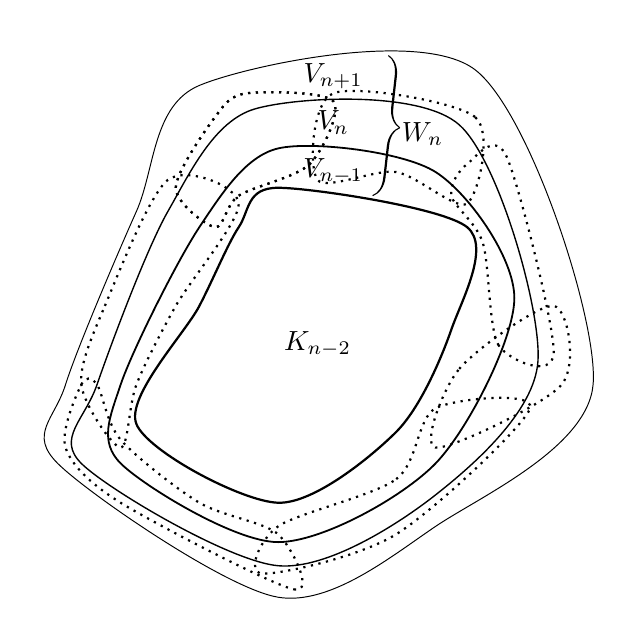
\begin{tikzpicture}
            \draw[line width=0.35] plot[smooth cycle] coordinates {
                (-0.8,1) (2,-0.7) (4,0.2) (6,2) (4.5,6) (1,5.8) (0.2,4.2) (-0.7,2)
            };
            \draw[line width=0.5] plot[smooth cycle] coordinates {
                (-0.5,1) (2,-0.3) (4,0.6) (5.3,2.3) (4.3,5.3) (1.7,5.5) (0.6,4.2) (-0.3,2)
            };
            \draw[line width=0.65] plot[smooth cycle] coordinates {
                (0,1) (2,0) (4,1) (5,3.1) (4,4.7) (2,5) (1,4) (0,2)
            };
            \draw[thick] plot[smooth cycle] coordinates {
                (0.2,1.5) (2,0.5) (3.5,1.4) (4.2,2.7) (4.4,4) (2,4.5) (1.5,4) (1,3)
            };
            \draw[thick, dotted] plot[smooth cycle] coordinates {
                (4.4,4.3) (4.5,5.4) (2.7,5.7) (2.5,4.6) (3.5,4.7)
            };
            \draw[thick, dotted] plot[smooth cycle] coordinates {
                (1.2,4) (0.7,4.5) (1.2,5.4) (1.6,5.7) (2.7,5.6) (2.4,4.8) (1.5,4.4)
            };
            \draw[thick, dotted] plot[smooth cycle] coordinates {
                (1.2,4) (0.7,4.5) (1.2,5.4) (1.6,5.7) (2.7,5.6) (2.4,4.8) (1.5,4.4)
            };
            \draw[thick, dotted] plot[smooth cycle] coordinates {
                (-0.5,2) (-0.2,3) (0.6,4.6) (1.5,4.3) (0.7,3) (0.2,2) (0,1.2)
            };
            \draw[thick, dotted] plot[smooth cycle] coordinates {
                (0,0.5) (2.2,-0.6) (2,0.1) (1,0.5) (0,1.3) (-0.3,2) (-0.5,2) (-0.7,1.2)
            };
            \draw[thick, dotted] plot[smooth cycle] coordinates {
                (2,0.2) (3.5,0.8) (4,1.7) (5.2,1.7) (3.5,0.1) (1.8,-0.4)
            };
            \draw[thick, dotted] plot[smooth cycle] coordinates {
                (4,1.2) (4.3,2.2) (5.5,3) (5.6,2)
            };
            \draw[thick, dotted] plot[smooth cycle] coordinates {
                (5.5,2.4) (4.8,2.5) (4.6,3.8) (4.2,4.4) (4.4,4.8) (4.9,4.9)
            };

            \node[anchor=north] at (2.5,2.8) {\(K_{n-2}\)};
            \node[anchor=north] at (2.7,5) {\(V_{n-1}\)};
            \node[anchor=north] at (2.7,5.6) {\(V_n\)};
            \node[anchor=north] at (2.7,6.2) {\(V_{n+1}\)};
            \draw[decorate,decoration={calligraphic
            brace, amplitude=7pt},thick] (3.4,6.18) -- (3.2,4.4) node[midway, yshift=-3pt,right=4pt] {\(W_n\)};
        \end{tikzpicture}
        \caption{The geometry of the finite subcover of \(V_n\subset W_n\) for some \(n\in\mathbb{N}\).}
        \label{fig:locallyfiniteopencoverexistence}
    \end{figure}Let \(K_{-1}=K_0=\emptyset,K_1,K_2,\cdots\subset\Omega\) exhaust \(\Omega\), with each \(K_n\) compact and \(K_n\subseteq \interior{K_{n+1}}\). For each \(n\in\mathbb{N}\), define \(W_n=\interior{K_{n+1}}\setminus K_{n-2}\), which is open, and \(V_n=K_n\setminus \interior{K_{n-1}}\), which is compact (as in \autoref{fig:locallyfiniteopencoverexistence}).

    By construction, \(V_n\subseteq W_n\) for all \(n\in\mathbb{N}\). The sets \(\{V_n\}\) form compact shells exhausting \(\Omega\), since \(\bigcup_{n\in\mathbb{N}}V_n=\Omega\).

    \(\forall n\in\mathbb{N}\) and \(\forall z\in V_n\), since \(W_n\) is an open set containing \(z\) and \(\mathfrak{B}\) is a basis, there exists \(U_{z,n}\in\mathfrak{B}\) such that \(z\in U_{z,n}\subseteq W_n\) (in short, \(U_{z,n}\) is an open neighborhood of \(z\) that is contained in \(W_n\)). The collection \(\cbraces{U_{z,n}}{z\in V_n}\) is an open cover of the compact set \(V_n\), so by the Heine-Borel Theorem (\autoref{thm:heineborel}) it admits a finite subcover of \(V_n\), as pictured in the dotted lines of \autoref{fig:locallyfiniteopencoverexistence}. That is, there exist finitely many points \(z_{n,1},\ldots,z_{n,k_n}\) such that \(V_n\subset\bigcup_{i=1}^{k_n}U_{z_{n,i},n}\subseteq W_n\).

    Let \(\{U_j\}\) be the collection formed by enumerating all such \(U_{z_{n,i},n}\) for \(n\in\mathbb{N}\) and \(i=1,\ldots,k_n\). Then \(\{U_j\}\subset\mathfrak{B}\) is a countable collection whose union covers \(\Omega\), proving~\ref{itm:locallyfiniteopencoverexistence_cover}.

    For \ref{itm:locallyfiniteopencoverexistence_localfiniteness}, let \(K\subset\Omega\) be compact. Then \(\exists N\in\mathbb{N}\) such that \(K\subset \interior{K_N}\), and hence \(K\) is disjoint from \(V_n\) for all \(n>N+1\). Since each \(V_n\) intersects only finitely many \(U_j\), it follows that \(K\) intersects only finitely many of the \(U_j\). Thus, the collection is \textit{locally finite}.
\end{proof}
\begin{remark}
    The property of local finiteness of an open collection \(S\) in \(\Omega\) is commonly stated as:

    \(\forall z\in\Omega\), there exists an open neighborhood of \(z\) intersecting finitely many sets in \(S\).

    Obviously, this assertion implies \ref{itm:locallyfiniteopencoverexistence_localfiniteness} in \autoref{lemma:locallyfiniteopencoverexistence}: let \(K\subset \Omega\) be compact, and for every \(z\in\Omega\), the collection of neighborhoods covers \(K\), and by the Heine--Borel Theorem (\autoref{thm:heineborel}), admits a finite subcover. Therefore, \(K\) intersects finitely many sets in \(S\). Conversely, \(\forall z\in\Omega\), there exists an open neighborhood \(V\ni z\) relatively compact in \(\Omega\). By assumption, \(\overline{V}\) intersects finitely many sets in \(S\), and since \(V\subset\overline{V}\), the conclusion follows.
\end{remark}
\begin{theorem}[Partition of Unity]\label{thm:partitionofunity}
    For a nonempty open set \(\Omega\subseteq\mathbb{C}\), let \(\cbraces{\Omega_k}_{k\in\mathbb{Z}_{\ge0}}\) be an open cover of \(\Omega\). Then there exists a set of bump functions, \(\alpha_1(z),\alpha_2(z),\ldots\in C^\infty(\mathbb{C})\) with compact support within \(\Omega\) satisfying
    \begin{enumerate}
        \item \(\forall j\in\mathbb{N}\), \(\exists k\in\mathbb{Z}_{\geq0}\) such that \(\supp\paren{\alpha_j}\subseteq\Omega_k\).\label{itm:partitionofunity_subordinate}
        \item The collection \(\qty{\supp\paren{\alpha_j}}\) is locally finite.\label{itm:partitionofunity_localfiniteness}
        \item \(\forall j\in\mathbb{N}\), \(0\leq\alpha_j\leq 1\).\label{itm:partitionofunity_nonnegativity}
        \item \(\forall z\in\Omega\), \(\sum_{j=1}^\infty \alpha_j(z)=1,\)\label{itm:itm:partitionofunity_partitionofunity}
    \end{enumerate} known as a \(C^\infty\) partition of unity subordinate to \(\cbraces{\Omega_k}_{k\in\mathbb{Z}_{\geq0}}\).
\end{theorem}
\begin{proof}
    By the openness of \(\Omega_k\), \(\forall z\in\Omega\), \(\exists r_z>0\) such that \(\overline{D\paren{z,r_z}}\subset\Omega_{k_z}\) for some \(k_z\in\mathbb{Z}_{\ge0}\).

    Then, \(\cbraces{D\paren{z,r}}{z\in\Omega, 0<r<r_z}\) forms an open basis of \(\Omega\). By \autoref{lemma:locallyfiniteopencoverexistence}, there exists a locally finite open cover \(\cbraces{D\paren{z_j,r_{z_j}}}\) of \(\Omega\), and since it is a subcollection of the basis, \[D\paren{z_j,r_{z_j}}\subset\overline{D\paren{z_j,r_{z_j}}}\subset\Omega_{k_{z_j}},\quad\forall j\in\mathbb{N}.\] The most trivial bump function has the form \[\theta(z)=
        \begin{cases}
            \exp\paren{\frac{1}{\abs{z}^2-1}} & \abs{z}<1   \\
            0                                 & \abs{z}\ge1
    \end{cases},\] which has the support \(\overline{D(0,1)}\). Define the function \(\theta_\varepsilon(z)=\varepsilon^{-2}\theta\qty(\frac{z}{\varepsilon})\) with the support \(\overline{D(0,\varepsilon)}\), which satisfies that \(\forall\varepsilon>0\), \[\int_{\mathbb{C}}\theta_\varepsilon(z)\ddx\wedge\ddy=1.\]
    Define a set of functions \(\cbraces{\beta_j(z)}_{j\in\mathbb{N}}\) with \(\beta_j(z)=\theta_{r_{z_j}}\paren{z-z_j}\), which is a bump function with \(\supp\qty(\beta_j)=\overline{D\paren{z_j, r_{z_j}}}\subset\Omega_{k_{z_j}}\).

    By the local finiteness of \(\qty{D\qty(z_j,r_{z_j})}\), there exists an open neighborhood \(V_z\) of each point \(z\in\Omega\) such that the set \(\cbraces{j}{V_z\cap D\qty(z_j,r_{z_j})\neq\emptyset}\) is finite. Since every open neighborhood of each point in \(\overline{D\qty(z_j,r_{z_j})}\) intersects \(D\qty(z_j,r_{z_j})\), it follows that every open set disjoint from \(D\qty(z_j,r_{z_j})\) is also disjoint from its closure. Since \(\overline{D\qty(z_j,r_{z_j})}\supset D\qty(z_j,r_{z_j})\), any open set intersecting \(D\qty(z_j,r_{z_j})\) will intersect \(\overline{D\qty(z_j,r_{z_j})}\). Therefore, \(\cbraces{j}{V_z\cap\overline{D\qty(z_j,r_{z_j})}\neq\emptyset}\) is finite. Equivalently, \(\cbraces{\supp\paren{\beta_j}}_{j\in\mathbb{N}}\) is locally finite on \(\Omega\).

    Consequently, \(\forall z_0\in\Omega\), there exists an open neighborhood \(V\ni z_0\) that intersects a finite number of sets in \(\cbraces{\supp\paren{\beta_j}}_{j\in\mathbb{N}}\). Then \(\forall z\in V\), the sum \[S(z)=\sum_{j=1}^\infty\beta_j(z)\] is a sum of finitely many terms and is therefore \(C^\infty\) at \(z_0\). Since the collection of supports exhausts \(\Omega\), \(S(z)\) is positive. Therefore, the sequence defined by \[\alpha_j(z)={\frac{\beta_j(z)}{S(z)}}\] is also \(C^\infty\) and is compactly supported in \(\Omega\). Furthermore, it satisfies \[\sum_{j=1}^\infty\alpha_j(z)=1.\]
\end{proof}
\begin{theorem}[Existence of Bump Functions]\label{thm:bumpfunctionexistence}
    Let \(\Omega\subset\mathbb{C}\) be open, \(K\subset\Omega\) be compact, and \(V\subseteq\Omega\) be an open neighborhood of \(K\). Then there exists a bump function \(\varphi\in C^\infty\paren{\mathbb{C}}\) with compact support contained in \(V\) such that \(\forall z\in\mathbb{C}\), \(0\leq\varphi(z)\leq 1\), and there exists an open neighborhood of \(K\) over which \(\varphi\equiv1\).
\end{theorem}
\begin{proof}
    Let \(V(K,\varepsilon)=\left\{z\in\mathbb{C}\,\middle|\,\inf_{\zeta\in K}\abs{\zeta-z}<\varepsilon\right\}\). In other words, \(z\) is within \(\varepsilon\) apart from \(K\).

    Then \(\exists\varepsilon>0\) such that \(K\subset V(K,\varepsilon)\subset V(K,2\varepsilon)\subseteq V\). Let \(\Omega_1=V(K,2\varepsilon)\) and \(\Omega_2=\Omega\setminus V(K,\varepsilon)\). Then there exists a \(C^\infty\) partition of unity \(\cbraces{\alpha_j(z)}_{j\in\mathbb{N}}\) of \(\Omega\) subordinate to the open cover \(\cbraces{\Omega_1,\Omega_2}\). Define a new function
    \[\varphi(z)=\sum_{\substack{j\in\mathbb{N}\\\supp{\alpha_j}\subseteq\Omega_1}}\alpha_j(z).\]
    It follows that \(\varphi\in C^\infty(\mathbb{C})\) with compact support in \(\Omega_1\). Since the support of every \(\alpha_j\) where \(j\in\mathbb{N}\) lies entirely either in \(\Omega_1\) or \(\Omega_2\), \[1=\sum_{\substack{j\in\mathbb{N}\\\supp{\alpha_j}\subseteq\Omega_2}}\alpha_j(z)+\varphi(z).\]
    When \(z\in\Omega_1\setminus\Omega_2=V(K,\varepsilon)\), the first summation vanishes, meaning that \(\varphi(z)\equiv1\) on the neighborhood \(V(K,\varepsilon)\) of \(K\). When \(z\in\Omega_2\setminus\Omega_1=\Omega\setminus V(K,2\varepsilon)\), \(\varphi(z)\) vanishes.
\end{proof}
\subsection{Zeros of a Holomorphic Function}
For a region \(U\subseteq\mathbb{C}\) and a holomorphic function \(f:U\to\mathbb{C}\), a point \(z_0\in U\) is a \textit{zero} of \(f\) if and only if \(f\paren{z_0}=0\). Furthermore, if \(f\) has the Taylor expansion at \(z_0\) of \[a_m\paren{z-z_0}^m+a_{m+1}\paren{z-z_0}^{m+1}+\cdots,\qquad m\in\mathbb{N},a_m\neq0,\] then the zero at \(z_0\) has multiplicity \(m\).

We will introduce a fundamental application of Liouville's Theorem (\autoref{thm:liouville}) below.
\begin{theorem}[Fundamental Theorem of Algebra]\label{thm:fundamentaltheoremofalgebra}
    Every non-constant polynomial \(p(z)\) with complex coefficients has at least one complex zero.
\end{theorem}
\begin{proof}
    For the sake of contradiction, suppose that \(p(z)\) has no complex zeros. Then the function \(f(z)=\frac{1}{p(z)}\) is continuous and entire, because \(p(z)\) has no zeros in \(\mathbb{C}\). Moreover, as \(z\to\infty\), \(p(z)\to\infty\), so \(f(z)\to 0\), and thus \(f(z)\) is bounded. By Liouville's Theorem (\autoref{thm:liouville}), every bounded entire function is constant. Thus, \(f(z)\) is constant, and so \(p(z)\) must also be constant. By contradiction, \(p(z)\) has at least one complex zero.
\end{proof}
\begin{theorem}\label{thm:identityaccumulationofzeros}
    Let \(U\subseteq\mathbb{C}\) be open and connected, and \(f:U\to\mathbb{C}\) be holomorphic over \(U\). Then if the set defined by \(S=\cbraces{z\in U\mid f(z)=0}\) has an accumulation point in \(U\), then \(f\equiv0\) over \(U\).
\end{theorem}
\begin{proof}
    Let \(\cbraces{z_n}_{n\in\mathbb{N}}\) be a subset of \(S\) and assume it has an accumulation point \(z_\infty\) in \(U\). Since \(f\) is holomorphic over \(U\), \(\exists\varepsilon>0\) such that \(f\) is holomorphic over \(D\paren{z_\infty,\varepsilon}\subseteq U\). Then over this disk, \(f\) has the Taylor expansion
    \begin{equation}\label{eq:identityaccumulationofzeros_taylorexpansion}
        f(z)=\sum_{n=0}^\infty a_n\paren{z-z_\infty}^n.
    \end{equation}
    By \autoref{def:accumulationpoint}, \(\exists N\in\mathbb{N}\) such that \(\forall n>N\), \(z_n\in D\paren{z_\infty,\varepsilon}\). Since \(z_n\) is a zero of \(f\), \(f\paren{z_n}=0\). Then, by the continuity of \(f\), \[\lim_{n\to\infty} f\paren{z_n}=f\paren{\lim_{n\to\infty}z_n}=f\paren{z_\infty}=0.\] Using this result in comparison to equation~\eqref{eq:identityaccumulationofzeros_taylorexpansion}, we get that \(a_0=0\).

    The function \(f_1(z)=\frac{f(z)}{z-z_\infty}\) has a Taylor expansion over \(D\paren{z_0,\varepsilon}\) of
    \[f_1(z)=\sum_{n=0}^\infty a_{n+1}\paren{z-z_\infty}^n.\]
    Let \(z=z_n\neq z_\infty\) for some \(n>N\). Then \(f_1\) vanishes, leaving \[0=a_1+\mathcal{O}_{n\to\infty}\paren{z_n-z_\infty}.\]
    Letting \(n\to\infty\), \(z_n\to z_\infty\), and \(a_1=0\). Define \(f_2(z)=\frac{f_1(z)}{z-z_\infty}\). Then, \[f_2(z)=\sum_{n=0}^\infty a_{n+2}\paren{z-z_\infty}^n.\]
    Similarly, \(a_2=0\). Letting \(f_n(z)=\frac{f(z)}{\paren{z-z_\infty}^n}\), the sequence \(\cbraces{a_n}_{n\in\mathbb{Z}_{\geq0}}\) vanishes, and \(f\equiv 0\) on \(D\paren{z_\infty,\varepsilon}\).

    Let \(\widetilde{S}=\cbraces{z\in U}{\forall n\in\mathbb{Z}_{\geq0}, f^{(n)}(z)=0}\).\ \(\forall z\in D\paren{z_\infty,\varepsilon}\), since \(f(z)\) locally vanishes (and has vanishing derivatives as a consequence), \(D\paren{z_\infty,\varepsilon}\subseteq \widetilde{S}\). Furthermore, \(\forall z'\in \widetilde{S}\), \(\exists\varepsilon'>0\) such that \(f(z)\) has a convergent Taylor series with vanishing coefficients on \(D(z',\varepsilon')\subseteq U\). Then \(f\equiv0\) on \(D\paren{z',\varepsilon'}\). Then \(\forall z\in D(z',\varepsilon')\), since \(f\) is constant at \(z\), it also has vanishing derivatives. It follows that \(D(z',\varepsilon')\subseteq \widetilde{S}\). Since every point in \(\widetilde{S}\) has an open neighborhood also in \(\widetilde{S}\), \(\widetilde{S}\) is open.

    It is evident that \(\forall k\in\mathbb{Z}_{\geq0}\), \(f^{(k)}\) is continuous in \(U\) by the holomorphy of \(f\). Let \(S_k=\cbraces{z\in U}{f^{(k)}(z)=0}\). For any sequence \(\cbraces{\widetilde{z}_n}\in S_k\) converging to some \(\widetilde{z}_\infty\in U\), by the continuity of \(f\), \[\lim_{n\to\infty} f^{(k)}\paren{\widetilde{z}_n}=f^{(k)}\paren{\lim_{n\to\infty}\widetilde{z}_n}=f^{(k)}\paren{z'_\infty}=0,\] and therefore \(\widetilde{z}_\infty\in S_k\). Thus, \(S_k\) contains all of its accumulation points in \(U\) and is therefore closed in \(U\) (if \(\widetilde{z}_\infty\notin U\), then it is no longer relevant; we are concerned about it being closed within \(U\)). Since \(\widetilde{S}=\bigcap_{k\in\mathbb{Z}_{\geq0}} S_k\) and each of \(S_k\) is closed in \(U\), \(\widetilde{S}\) is the intersection of closed sets and consequently closed.

    Since \(\widetilde{S}\) is nonempty and clopen in the connected set \(U\), \(\widetilde{S}=U\) (by \autoref{thm:connectedtopologicalspaceclopensets}). It follows that \(f\equiv 0\) on \(U\).
\end{proof}
\begin{remark}
    This is a trivial property of holomorphic functions that allows for the uniqueness of analytic continuations. It is oftentimes stated in the form below:
\end{remark}
\begin{theorem}[Identity Theorem]\label{thm:identity}
    Let \(U\subseteq\mathbb{C}\) be open and connected, and define \(f(z)\) and \(g(z)\) to be two holomorphic functions on \(U\). For a set \(S\subseteq U\) with an accumulation point in \(U\), if \(f\equiv g\) on \(S\), then \(f\equiv g\) on \(U\).
\end{theorem}
\begin{proof}
    Let \(h=f-g\) be holomorphic over \(U\). Since \(S\) has an accumulation point in \(U\), and \(h\equiv 0\) over \(S\), then by \autoref{thm:identityaccumulationofzeros}, \(h\equiv 0\) over \(U\).
\end{proof}
\begin{theorem}[Argument Principle for Holomorphic Functions]\label{thm:argumentprincipleholomorphic}
    Let \(U\subseteq\mathbb{C}\) be a region and \(f:U\to\mathbb{C}\) be holomorphic. Let \(\gamma\subset U\) be a simple, closed, positively oriented curve that is null-homotopic in \(U\). If \(f\) has no zeros on \(\gamma\), then \(f\) has finitely many zeros in the region bounded by \(\gamma\), and this number, counting multiplicities, is given by
    \[k=\frac{1}{2\piup\ii}\oint_{\gamma}\frac{f'(z)}{f(z)}\ddz.\]
    Let \(\Gamma\) be the image of \(\gamma\) under the map \(w=f(z)\). Then \(k=\frac{1}{2\piup}\Delta_\Gamma\arg(w)\), where \(\Delta_\Gamma\arg(w)\) denotes the total change in argument of \(w\) as it traverses \(\Gamma\).
\end{theorem}
\begin{proof}
    Let \(z_1,\ldots,z_n\) be the distinct zeros of \(f\) enclosed by \(\gamma\) with the respective multiplicities \(k_1,\ldots,k_n\). Choose disjoint disks \(D\qty(z_j,\varepsilon_j)\) centered at each \(z_j\) with radii \(\varepsilon_j>0\), each contained in the interior of \(\gamma\) and avoiding \(\gamma\). The function \[\frac{f'(z)}{f(z)}\]
    is holomorphic on the domain \[\mathrm{int}\paren{\gamma}\setminus\bigcup_{j=1}^n \overline{D\qty(z_j,\varepsilon_j)},\]
    where \(\mathrm{int}(\gamma)\) denotes the interior relative to \(\gamma\). The oriented boundary of this domain is \(\gamma^+\cup\bigcup_{j=1}^n\partial D\paren{z_j,\varepsilon_j}^-\). By Cauchy--Goursat (\autoref{thm:cauchygoursattheorem}),
    \[\int_{\gamma^+\cup\bigcup_{j=1}^n\partial D\paren{z_j,\varepsilon_j}^-}\frac{f'(z)}{f(z)}\ddz=0,\]
    which rearranges to
    \[\oint_{\gamma^+}\frac{f'(z)}{f(z)}\ddz=\sum_{j=1}^n\oint_{\partial D\paren{z_j,\varepsilon_j}^+}\frac{f'(z)}{f(z)}\ddz.\]
    Near each \(z_j\), express \(f(z)=\paren{z-z_j}^{k_j}h_j(z)\) where \(h_j\) is holomorphic and non-vanishing on \(D\paren{z_j,\varepsilon_j}\). Differentiation yields
    \[f'(z)=k_j\paren{z-z_j}^{k_j-1}h_j(z)+\paren{z-z_j}^{k_j}h_j'(z),\] and thus
    \[\frac{f'(z)}{f(z)}=\frac{k_j}{z-z_j}+\frac{h_j'(z)}{h_j(z)}.\]
    Since \(h_j\) is holomorphic and non-vanishing on \(D\paren{z_j,\varepsilon_j}\), the function \(\frac{h_j'}{h_j}\) is holomorphic there. By the Cauchy--Goursat Theorem,
    \[\oint_{\partial D\paren{z_j,\varepsilon_j}}\frac{h_j'(z)}{h_j(z)}\ddz=0.\]
    The Cauchy--Goursat Formula (\autoref{thm:cauchygoursatformula}) gives
    \[\oint_{\partial D\paren{z_j,\varepsilon_j}}\frac{k_j}{z-z_j}\ddz=2\piup \ii k_j.\]
    Combining results,
    \[\oint_{\gamma}\frac{f'(z)}{f(z)}\ddz=\sum_{j=1}^n2\piup \ii k_j=2\piup \ii k.\]
    Finally, parametrize \(\Gamma\) by \(w=f(z)\). Then \(\dd{w}=f'(z)\ddz\), and
    \[k=\frac{1}{2\piup\ii}\oint_{\Gamma}\frac{\dd{w}}{w}=\frac{1}{2\piup\ii}\Delta_\Gamma\log(w)=\frac{1}{2\piup}\Delta_\Gamma\arg(w),\] which proves the result.
\end{proof}
This profound result proves that the number of zeros of a holomorphic function enclosed by a closed curve is also the number of times the image of the curve winds around the origin.
\begin{theorem}\label{thm:hurwitzsimplecase}
    Let \(\cbraces{f_n(z)}\) be a sequence of holomorphic functions on the open set \(U\subseteq\mathbb{C}\) that uniformly converges to \(f(z)\) on every compact subset of \(U\). If \(\forall n\in\mathbb{N}\), \(f_n(z)\) has no zeros in \(U\), then \(f\) is either identically 0 or has no zeros in \(U\).
\end{theorem}
\begin{proof}
    By the holomorphy of \(f_n(z)\), for any simple closed rectifiable curve \(\gamma\subset U\) (whose interior is a subset of \(U\)), by the Cauchy--Goursat Theorem (\autoref{thm:cauchygoursattheorem}), \[\oint_{\gamma}f_n(\zeta)\ddzeta=0.\] Since \(\gamma\) is a subset of any compact subset of \(U\), \(\cbraces{f_n(\zeta)}\) uniformly converges on \(\gamma\), and by \autoref{thm:limitintegralswitch},
    \begin{equation}
        \lim_{n\to\infty}\oint_{\gamma}f_n(\zeta)\ddzeta=\oint_{\gamma}\lim_{n\to\infty}f_n(\zeta)\ddzeta=\oint_{\gamma}f(\zeta)\ddzeta=0.\label{eq:hurwitzsimplecase_integrallimitswitchforholomorphy}
    \end{equation}
    Then by Morera's Theorem (\autoref{thm:morera}), \(f(z)\) is holomorphic, and \(f'(z)\) is holomorphic. We aim to show that \(f'_n(z)\rightrightarrows f'(z)\).

    Let \(K\subset U\) be arbitrary and compact and \(V\supset K\) be open and relatively compact in \(U\). Since \(\cbraces{f'_n(z)}\) is holomorphic, by \autoref{crl:nthderivativeboundedsupremum}, there exists a finite constant \(c>0\) such that \[\lim_{n\to\infty}\sup_{z\in K}\abs{f'_n(z)-f'(z)}\leq c\lim_{n\to\infty}\sup_{z\in V}\abs{f_n(z)-f(z)}.\]

    By the definition of uniform convergence, the right-hand side approaches 0, and \(\cbraces{f'_n(z)}\) is then uniformly convergent to \(f'(z)\) by the same reasoning.

    Through the proof of \autoref{thm:identityaccumulationofzeros}, if \(f\not\equiv0\) over \(U\), then the zeros of \(f\) do not have an accumulation point in \(U\) and are therefore discrete. In this case, let \(\gamma\subset U\) be a curve that does not pass through the zeros of \(f\). Since each function in the sequence \(f_n\) does not contain zeros in \(U\), by the Argument Principle, (\autoref{thm:argumentprincipleholomorphic}),
    \begin{equation}
        \lim_{n\to\infty}\oint_{\gamma}\frac{f_n'(z)}{f_n(z)}\ddz=0.\label{eq:hurwitzsimplecase_argumentprinciple}
    \end{equation}
    Since \(f\) and \(f'\) are holomorphic over \(\gamma\), by \autoref{thm:continuousfunctionboundedoncompact}, there exists a finite value \(M>0\) such that \(\forall z\in\gamma\), \(\max\paren{\abs{f(z)},\abs{f'(z)}}<M\).

    Since \(\gamma\) does not pass through the zeros of \(f\), \(\exists\lambda>0\) such that \(\forall z\in\gamma\), \(\abs{f(z)}>\lambda\). By the uniform convergence of \(\cbraces{f_n(z)}\), \(\exists N\in\mathbb{N}\) such that
    \[\abs{f_n(z)-f(z)}<\frac{\lambda}{2},\quad\forall n>N,\forall z\in\gamma.\]
    Then \(\abs{f_n(z)}>\frac{\lambda}{2}\) on \(\gamma\). Hence, \(\frac{1}{f_n(z)}\) and its limit are uniformly bounded; \[\abs{\frac{1}{f(z)}}<\frac{1}{\lambda},\quad\abs{\frac{1}{f_n(z)}}<\frac{2}{\lambda},\quad\forall z\in\gamma,\forall n>N.\]
    Then,
    \begin{align*}
        \abs{\frac{f'}{f}-\frac{f'_n}{f_n}}                                               & =\abs{\frac{f'f_n-f'_n f}{f_n f}}                                                                         \\
        & <2\frac{\abs{f'f_n-f'f}+\abs{f'f-f'_n f}}{\lambda^2}                                                     \\
        & <\frac{2M}{\lambda^2}\cdot\paren{\abs{f_n-f}+\abs{f'-f'_n}}.                                            \\
        \sup_{z\in\gamma}\abs{\frac{f'(z)}{f(z)}-\frac{f'_n(z)}{f_n(z)}}                  & \leq\frac{2M}{\lambda^2}\paren{\sup_{z\in\gamma}\abs{f_n(z)-f(z)}+\sup_{z\in\gamma}\abs{f'(z)-f'_n(z)}} \\
        \lim_{n\to\infty}\sup_{z\in\gamma}\abs{\frac{f'(z)}{f(z)}-\frac{f'_n(z)}{f_n(z)}} & \leq\frac{2M}{\lambda^2}\paren{\lim_{n\to\infty}\sup_{z\in\gamma}\abs{f_n(z)-f(z)}+\abs{f'(z)-f'_n(z)}} \\
        & =0.
    \end{align*}
    Therefore, \(\frac{f'(z)}{f(z)}\) is uniformly convergent on \(\gamma\). By \autoref{thm:limitintegralswitch}, we can pass the limit through the integral in equation~\eqref{eq:hurwitzsimplecase_argumentprinciple}. Then,
    \[\lim_{n\to\infty}\oint_\gamma \frac{f'_n(z)}{f_n(z)}\ddz=\oint_\gamma \frac{f'(z)}{f(z)}\ddz=0.\] By the Argument Principle, (\autoref{thm:argumentprincipleholomorphic}), \(f(z)\) has no zeros in the interior of \(\gamma\). Since \(\gamma\) was arbitrarily chosen, either \(f(z)\equiv 0\) on \(U\) or has no zeros in \(U\).
\end{proof}
\begin{theorem}[Rouché]\label{thm:rouche}
    Let \(U\subseteq\mathbb{C}\) be open and \(f,g\) be two holomorphic functions over \(U\). Let \(\gamma\subset U\) be a simple, closed, rectifiable curve, and \(\forall z\in\gamma\)
    \begin{equation}
        \abs{f(z)-g(z)}<\abs{f(z)}\label{eq:rouche}.
    \end{equation} Then \(f\) and \(g\) have the same number of zeros enclosed by \(\gamma\) and do not vanish on \(\gamma\).
\end{theorem}
\begin{proof}
    It is obvious that \(g(z)\) has no zeros on \(\gamma\). Otherwise, \(\exists z_0\in\gamma\) such that \(g\paren{z_0}=0\), implying that \(\abs{f\paren{z_0}}<\abs{f\paren{z_0}}\) which is impossible. Similarly, \(f(z)\) has no zeros on \(\gamma\), since \(\abs{g(z)}<0\) is an impossibility.

    Let \(k_f\) and \(k_g\) denote the number of zeros of \(f\) and \(g\) enclosed by \(\gamma\), respectively. By the Argument Principle (\autoref{thm:argumentprincipleholomorphic}),
    \begin{align*}
        k_g-k_f & =\int_{\gamma}\frac{g'(z)}{g(z)}\ddz-\int_\gamma\frac{f'(z)}{f(z)}\ddz                                                    \\
        & =\int_\gamma\frac{g'(z)f(z)-f'(z)g(z)}{g(z)f(z)}\ddz=\int_\gamma\frac{\qty(\frac{g(z)}{f(z)})'}{\frac{g(z)}{f(z)}}\ddz.
    \end{align*}
    Let \(w=h(z)=\frac{g(z)}{f(z)}\) with \(\Gamma=h(\gamma)\). Then, \[k_g-k_f=\int_\Gamma\frac{\dd{w}}{w}.\]
    From equation~\eqref{eq:rouche}, by dividing both sides by \(f(z)\), we obtain \(\abs{w-1}<1\). Then \(\Gamma\) lies in the open disk \(D(1,1)\), which will never intersect or enclose 0. Then by \autoref{lemma:cauchyintegraltheoremoversimplyconnectedset}, \[k_g-k_f=\int_\Gamma\frac{\dd{w}}{w}=0,\] as desired.
\end{proof}
By the Fundamental Theorem of Algebra (\autoref{thm:fundamentaltheoremofalgebra}), any polynomial in the form \(p(z)=\sum_{k=0}^n a_kz^k\) (\(n\in\mathbb{N}\), \(a_n\neq 0\), \(a_k\in\mathbb{C}\) where \(k=1,\ldots n\)) has at least one complex zero. Consider the function \(q(z)=a_nz^n\), with a zero at \(z=0\) with multiplicity \(n\). By Rouché's Theorem (\autoref{thm:rouche}), since \(\exists R\in\mathbb{R}\) such that \(\abs{q(z)-p(z)}=\abs{\sum_{k=0}^{n-1}a_k z^k}<\abs{a_n z^n}\) over \(\abs{z}=R\), \(p\) and \(q\) have the same number of zeros, counting multiplicity.
\begin{theorem}\label{thm:hurwitzshifts}
    Let \(U\subseteq\mathbb{C}\) be open and connected, and \(f(z)\) be holomorphic and non-constant on \(U\).

    If \(z_0\in U\) and \(w_0=f\qty(z_0)\), and the multiplicity of the zero at \(z_0\) of \(f-w_0\) is \(m\), then for all \(\rho>0\) such that \(f-w_0\) is non-vanishing on \(\overline{D\qty(z_0,\rho)}\setminus\qty{z_0}\), \(\exists\delta>0\) such that \(\forall\xi\in D\qty(w_0,\delta)\), \(f-\xi\) has \(m\) zeros in \(D\qty(z_0,\rho)\), counting multiplicity.
\end{theorem}
\begin{proof}
    The zero at \(z_0\) is isolated by \autoref{thm:identityaccumulationofzeros}. Furthermore, \(\abs{f-w_0}\) is continuous on \(\partial D\qty(z_0,\rho)\) and attains a positive infimum \(\delta\). In other words, on this set, \(\abs{f-w_0}\geq\delta\). Hence, \(\forall \xi\in D\qty(w_0,\delta)\), we have \(\abs{\xi-w_0}<\delta\leq\abs{f(z)-w_0}\) for any \(z\in\partial D\qty(z_0,\rho)\).

    By Rouché's Theorem, since \(\abs{\qty(f(z)-w_0)-\qty(f(z)-\xi)}<\abs{f(z)-w_0}\), it follows that \(f-\xi\) and \(f-w_0\) have the same number of zeros in \(D\qty(z_0,\rho)\).
\end{proof}
We also have the following generalization of \autoref{thm:hurwitzsimplecase}, which is a heuristic restatement of \autoref{thm:hurwitzshifts}:
\begin{theorem}[Hurwitz]\label{thm:hurwitz}
    Let \(U\subseteq\mathbb{C}\) be an open and connected set, and suppose \(\qty{f_n(z)}_{n\in\mathbb{N}}\) is a holomorphic function sequence that uniformly converges to a non-constant function \(f(z)\) on all compact sets of \(U\).

    If \(z_0\in U\) and \(w_0=f\qty(z_0)\), and the multiplicity of the zero at \(z_0\) of \(f-w_0\) is \(m\), then for all \(\rho>0\) such that \(f-w_0\) is non-vanishing on \(\overline{D\qty(z_0,\rho)}\setminus\qty{z_0}\), \(\exists N\in\mathbb{N}\) such that \(\forall n>N\), \(f_n-w_0\) has \(m\) zeros in \(D\qty(z_0,\rho)\), counting multiplicity.
\end{theorem}
\begin{proof}
    The zero at \(z_0\) is isolated by \autoref{thm:identityaccumulationofzeros}. Furthermore, \(\abs{f-w_0}\) is continuous on \(\partial D\qty(z_0,\rho)\) and attains a positive infimum \(\delta\). In other words, on this set, \(\abs{f-w_0}\geq\delta\). By uniform convergence, \(\exists N\in \mathbb{N}\) such that \(\forall n>N\), we have \(\abs{f(z)-f_n\qty(z)}<\delta\leq\abs{f(z)-w_0}\) for any \(z\in\partial D\qty(z_0,\rho)\).

    By Rouché's Theorem, since \(\abs{\qty(f(z)-w_0)-\qty(f_n(z)-w_0)}<\abs{f(z)-w_0}\), it follows that \(f_n-w_0\) and \(f-w_0\) have the same number of zeros in \(D\qty(z_0,\rho)\).
\end{proof}
\subsection{Further Properties of Holomorphic Functions}
A useful corollary of \autoref{thm:cauchygoursatformula} is the Maximum Modulus Principle.

Before the theorem, we first introduce the mean-value property of holomorphic functions.
\begin{lemma}\label{lemma:holomorphicmeanvalueproperty}
    Let \(U\subseteq\mathbb{C}\) be open and simply connected, and let \(f:U\to\mathbb{C}\) be holomorphic. Then \(\forall z\in U\) and \(\forall \varepsilon>0\) such that \(\overline{D(z,\varepsilon)}\subset U\), \(f(z)\) is the average of \(f(\zeta)\) where \(\zeta\in D(z,\varepsilon)\) is uniform. In other words, \[f(z)=\frac{1}{2\piup\varepsilon}\int_{\partial D(z,\varepsilon)}f(\zeta)\abs{\dd{\zeta}}.\]
\end{lemma}
\begin{proof}
    By the Cauchy--Goursat Formula (\autoref{thm:cauchygoursatformula}), \[f(z)=\frac{1}{2\piup\ii}\int_{\partial D(z,\varepsilon)}\frac{f(\zeta)}{\zeta-z}\ddzeta=\frac{1}{2\piup}\int_0^{2\piup}f\paren{z+\varepsilon \ee^{\ii t}}\dd{t}.\]
    Observe that
    \begin{align*}
        f(z)=\frac{1}{2\piup\varepsilon}\int_{\partial D(z,\varepsilon)}f(\zeta)\abs{\dd{\zeta}} & =\frac{1}{2\piup\varepsilon}\int_{0}^{2\piup}f\paren{z+\varepsilon \ee^{\ii t}}\abs{\ii\varepsilon \ee^{\ii t}\dd{t}} \\
        & =\frac{1}{2\piup}\int_{0}^{2\piup}f\paren{z+\varepsilon \ee^{\ii t}}\dd{t},
    \end{align*}
    and the conclusion follows.
\end{proof}
Since the real and imaginary parts of holomorphic functions are real-valued harmonic functions, they also satisfy the mean-value property. Furthermore, if a real continuous function satisfies the mean-value property, it is harmonic (to be proved in \autoref{thm:meanvaluepropertysolutionsareharmonic}). This equivalence allows for the alternative definition of harmonic functions.
\begin{theorem}[Maximum Modulus Principle]\label{thm:maximummodulus}
    Let \(f(z)\) be holomorphic on an open connected region \(U\subseteq\mathbb{C}\). If \(\exists z_0\in U\) and an open neighborhood \(V\subseteq U\) of \(z_0\) such that \(\forall z\in V\), \(\abs{f\paren{z_0}}\geq\abs{f(z)}\), then \(f\) is a constant function on \(U\).
\end{theorem}
\begin{proof}
    Assume that \(z_0\) exists. We will first prove that the set \[S=\cbraces{z}{f(z)=f\paren{z_0},z\in V}\]
    is all of \(V\). This is equivalent to proving that \(S\) is nonempty, open, and closed in \(V\).

    Since \(z_0\in S\), the first condition is satisfied (nonemptiness). For any sequence \(\cbraces{z_n}\in S\) converging to some \(z_\infty\in V\), by the continuity of \(f\), \[\lim_{n\to\infty} f\paren{z_n}=f\paren{\lim_{n\to\infty}z_n}=f\paren{z_\infty}=0,\] and \(z_\infty\in S\). Thus, \(S\) contains all of its accumulation points in \(V\) and is therefore closed (if \(z_\infty\notin V\), then it is no longer relevant; we are concerned with it being closed within \(V\)).

    Since \(S\subseteq V\) and \(V\) are both open, \(\forall z\in S\), \(\exists\lambda>0\) such that \(D(z,\lambda)\subseteq V\). By \autoref{lemma:holomorphicmeanvalueproperty}, \(\forall 0<\varepsilon<\lambda\),
    \begin{align*}
        |f(z)| & =\abs{\frac{1}{2\piup}\int_0^{2\piup}f\paren{z+\varepsilon \ee^{\ii t}}\dd{t}}\leq \frac{1}{2\piup}\int_0^{2\piup}\abs{f\paren{z+\varepsilon \ee^{\ii t}}}\dd{t} \\
        & \leq\frac{1}{2\piup}\int_0^{2\piup}\abs{f(z)}\dd{t}=\abs{f(z)}.
    \end{align*}
    It follows that all inequalities above are equalities, or that
    \begin{align*}
        |f(z)| & =\abs{\frac{1}{2\piup}\int_0^{2\piup}f\paren{z+\varepsilon \ee^{\ii t}}\dd{t}}=\frac{1}{2\piup}\int_0^{2\piup}\abs{f\paren{z+\varepsilon \ee^{\ii t}}}\dd{t} \\
        & =\frac{1}{2\piup}\int_0^{2\piup}\abs{f(z)}\dd{t}=\abs{f(z)}.
    \end{align*}
    From the equality of the last two integrals, \(\int_{0}^{2\piup}\qty(\abs{f(z)}-\abs{f\paren{z+\varepsilon \ee^{\ii t}}})\dd{t}=0\). Since this integrand is strictly non-negative, we have equality. Thus, \(\forall z\in S\), \(\exists\lambda>0\) such that \(D\paren{z,\lambda}\subseteq S\). In other words, every \(z\in S\) has an open neighborhood that also lies in \(S\). Therefore, \(S\) is open and \(S=V\) as it is a nonempty clopen subset. Since \(V\) is nonempty and open, it has an accumulation point in \(U\). It follows that \(f(z)\equiv f\paren{z_0}\) over \(U\) by the Identity Theorem (\autoref{thm:identity}).
\end{proof}
\begin{remark}
    If \(f\) is holomorphic and non-constant on an open region \(U\subseteq\mathbb{C}\), then for any compact set \(K\subset U\), the maximum of \(f\) in \(K\) lies on \(\partial K\). Otherwise, \(f\) would attain a maximum at some \(z\in \interior{K}\), and contradict the statement of \autoref{thm:maximummodulus} under the assumption of being non-constant.
\end{remark}
A similar theorem exists for real-valued harmonic functions. The proof follows in the same way as the one for holomorphic functions. We will state it formally below.
\begin{theorem}\label{thm:maximumprincipleforrealharmonicfunctions}
    Let \(U\subseteq\mathbb{C}\) be open and connected and let \(f:U\to\mathbb{R}\) be harmonic. If \(\exists z_0\in U\) and a neighborhood \(V\subseteq U\) of \(z_0\) such that \(\forall z\in V\), either \(f(z)\geq f\qty(z_0)\) completely or \(f(z)\leq f\qty(z_0)\) completely, then \(f\) is constant on \(U\).
\end{theorem}

As a matter of fact, the theorem follows for any continuous function satisfying the mean-value property.
\subsubsection{The Group of Holomorphic Automorphisms on the Unit Disk}
The following important result can be directly obtained from the Maximum Modulus Principle.
\begin{lemma}[Schwarz]\label{lemma:schwarz}
    If \(f:\mathbb{D}\to\mathbb{D}\) is holomorphic and \(f(0)=0\), then \[\abs{f(z)}\leq\abs{z},\quad\abs{f'(0)}\leq 1.\]
    Any one of the inequalities becomes equalities if and only if \(f(z)\) is in the form of \(z\ee^{\ii\tau}\), where \(\tau\in\mathbb{R}\). In other words, \(f\) is a pure rotation.
\end{lemma}
\begin{proof}
    Define the auxiliary function \[g(z)=
        \begin{cases}
            \frac{f(z)}{z} & z\neq0 \\
            f'(0)          & z=0
    \end{cases}.\]
    Because \(\lim_{z\to0}\frac{f(z)}{z}=f'(0)\), \(g(z)\) is holomorphic on \(\mathbb{D}\). Since \(f\) is an automorphism on the open disk, \(\forall\abs{z}<1\), \(\abs{f(z)}<1\). By the Maximum Modulus Principle \autoref{thm:maximummodulus}, \(\forall0<\varepsilon<1\), \(\forall z\in D(0,\varepsilon)\), \[\abs{g(z)}\leq\max_{z_\varepsilon\in \partial D(0,\varepsilon)}\frac{\abs{f\paren{z_\varepsilon}}}{\varepsilon}<\frac{1}{\varepsilon}.\] As \(\varepsilon\to 1^-\), we obtain that \(\forall z\in \mathbb{D}\), \(\abs{g(z)}\leq 1\), or that \(\abs{f(z)}\leq\abs{z}\). Let \(z=0\). Then we get \(\abs{g(0)}=f'(0)\leq 1\).

    For the sake of the equality condition, assume \(|f(z)|=|z|\). Then \(\abs{g(z)}\equiv 1\) on the unit open disk. By \autoref{thm:maximummodulus}, \(g(z)=\exp(\ii\tau)\) where \(\tau\in\mathbb{R}\) and \(f(z)=z\exp(\ii\tau)\) on \(\mathbb{D}\).

    Next, assume only that \(\abs{f'(0)}=1\). It follows that \(\abs{g(0)}=1\). Since \(\abs{g(z)}\leq 1\) for all \(z\in \mathbb{D}\), it follows from \autoref{thm:maximummodulus} that \(g\) is constant with magnitude 1, or in the form of \(\exp(\ii\tau)\), where \(\tau\in\mathbb{R}\) is a constant. Consequently, \(f(z)=z\exp(\ii\tau)\).
\end{proof}
To discuss the main topic of this section, we will first introduce the concept of a \textit{group}.
\begin{definition}[Group]\label{def:group}
    A group is a nonempty set \(G\) and a binary operation (we will denote this as \(*\)) satisfying the four \textit{group axioms}:
    \begin{itemize}
        \item Closure: \(\forall a,b\in G\), \(a*b\in G\).
        \item Associativity: \(\forall a,b,c\in G\), \((a*b)*c=a*(b*c)\).
        \item Identity Element: \(\exists e\in G\) such that \(\forall a\in G\), \(a*e=e*a=a\). Note that \(e\) is unique; if \(e,f\in G\) were both identity elements, then \(e*f=f*e=e=f\), and are equal.
        \item Inverse Element: \(\forall a\in G\), \(\exists a^{-1}\in G\) such that \(a*a^{-1}=e=a^{-1}*a\), where \(e\) is the identity element. Note that \(a^{-1}\) is unique. Assume \(b,c\) were both inverses of \(a\). Then, \(b=b*e=b*(a*c)=(b*a)*c=c\), and are equal.
    \end{itemize}
    A \textit{subgroup} \(H\) of \(G\) is a subset of \(G\) that is also a group under the same operation as \(G\). This relationship is denoted by \(H\leq G\) or \(H<G\) for \textit{proper subgroups}.
\end{definition}

If \(U\subseteq\mathbb{C}\) is connected and \(f:U\to U\) is holomorphic on \(U\) and bijective, \(f\) is a \textit{holomorphic automorphism} of \(U\). The \textit{group of holomorphic automorphisms} on \(U\) is denoted by \(\Aut(U)\), which is the set of all holomorphic automorphisms such as \(f\), with the operation of composition (\(f\circ g\)).

First we will show that \(\forall a\in \mathbb{D}\),
\begin{equation}
    \varphi_a(z)=\frac{z-a}{1-\overline{a}z}\in\Aut( \mathbb{D}).\label{eq:mobiustransformationgroupofholomorphicautomorphismsunitdisk_statement}
\end{equation}
Firstly, the function is holomorphic on \(\mathbb{D}\) as \(|z|\le1\), \(\abs{\overline{a}}<1\), the denominator never vanishes. Additionally, \(\varphi_a(a)=0\).

First, we will observe the image of \(\partial \mathbb{D}\). Let \(\abs{z}=1\). Then,
\[\abs{\varphi_a(z)}=\abs{\frac{1}{z}}\abs{\frac{z-a}{\frac{1}{z}-\overline{a}}}=\abs{\frac{z-a}{\overline{z}-\overline{a}}}=1.\]
Therefore, the image of \(\partial \mathbb{D}\) lies on \(\partial \mathbb{D}\), and since \(f\) is holomorphic and non-constant, by the Maximum Modulus Principle (\autoref{thm:maximummodulus}), for any \(\abs{z}<1\), \(\abs{\varphi_a(z)}<1\). Therefore, \(f\) maps \(\mathbb{D}\) to \(\mathbb{D}\). We next aim to show that \(f:\mathbb{D}\to \mathbb{D}\) is bijective.

Let us first confirm injectivity. \(\forall z_1,z_2\in \mathbb{D}\), we will observe when \[\frac{z_1-a}{1-\overline{a}z_1}=\frac{z_2-a}{1-\overline{a}z_2}\] is satisfied. It follows that
\begin{gather*}
    \qty(z_1-a)\qty(1-\overline{a}z_2)=\qty(z_2-a)\qty(1-\overline{a}z_1),\\
    z_1-a-\overline{a}z_1z_2+\abs{a}^2z_2=z_2-a-\overline{a}z_1z_2+\abs{a}^2z_1.
\end{gather*}
Then, \[\abs{a}^2\paren{z_2-z_1}=z_2-z_1.\Longleftrightarrow\qty(|a|^2-1)\qty(z_2-z_1)=0.\] Since \(\abs{a}<1\), then \(\abs{a}^2-1\neq0\), and we get \(z_2-z_2=0\). This proves the univalence of \(\varphi_a(z)\).

Next, we will solve for the inverse of \(\varphi_a\). Let \(z=\varphi_a(w)=\frac{w-a}{1-\overline{a}w}\). Then,
\begin{equation}
    z-\overline{a}zw=w-a\Longleftrightarrow w=\frac{z+a}{1+\overline{a}z}.\label{eq:inversemobiustransformation}
\end{equation}
It follows that \(\varphi_{-a}=\qty(\varphi_a)^{-1}\). Thus \(\varphi_a\) is surjective and a bijective automorphism. It follows that equation~\eqref{eq:mobiustransformationgroupofholomorphicautomorphismsunitdisk_statement} is true. Functions in the form of \(\varphi_a\) (where \(a\in \mathbb{D}\)) are known as \textit{Möbius transformations}, and the group of all such transformations is known as the \textit{Möbius transformation group on the unit disk}, which is a subgroup of \(\Aut(\mathbb{D})\). Functions in the form of \(\rho_\tau(z)=z\exp(\ii\tau)\), where \(\tau\in\mathbb{R}\) is constant, form a group known as the \textit{rotation group}, which is also a subgroup of \(\Aut(\mathbb{D})\).
\begin{theorem}[The Holomorphic Automorphism Group on the Unit Disk]\label{thm:holomorphicautomorphismgrouponunitdisk}
    \(\forall f\in \Aut(\mathbb{D})\), \(f\) is a composition between a Möbius transformation and a rotation. In other words, \(\exists |a|<1\) and \(\exists\tau\in\mathbb{R}\) such that \[f(z)=\varphi_a\circ\rho_\tau(z).\]
\end{theorem}
\begin{proof}
    Define the auxiliary function \(\psi(z)=\varphi_{f(0)}\circ f(z)\). It follows that \(\psi\in\Aut(\mathbb{D})\). Furthermore, \(\psi(0)=\varphi_{f(0)}\circ f(0)=0\).

    By the Schwarz Lemma (\autoref{lemma:schwarz}), \(\qty|\psi'(0)|\leq1\). Since \(\psi^{-1}\in\Aut(\mathbb{D})\) with \(\psi^{-1}(0)=0\), \(\abs{\qty(\psi^{-1})'(0)}\leq1\). Then, \[\abs{\qty(\psi^{-1})'(0)}=\frac{1}{\psi'\qty(\psi^{-1}(0))}=\frac{1}{\psi'(0)}\leq 1.\]
    Then, \(\abs{\psi'(0)}=1\), and by the equality statement of \autoref{lemma:schwarz}, \(\psi(z)=z\ee^{\ii\tau}=\rho_\tau(z)\) for some constant \(\tau\in\mathbb{R}\), and \(f(z)=\varphi_{f(0)}^{-1}\circ\rho_\tau(z)\). By equation~\eqref{eq:inversemobiustransformation}, it follows that \(f(z)=\varphi_{-f(0)}\circ\rho_\tau(z)\).
\end{proof}
As a direct consequence of \autoref{thm:holomorphicautomorphismgrouponunitdisk}, we have the following result:
\begin{lemma}[Schwarz--Pick Lemma]\label{lemma:schwarzpick}
    Let \(f:\mathbb{D}\to \mathbb{D}\) be holomorphic. \(\forall z_1,z_2\in \mathbb{D}\), let \(w_1=f\qty(z_1)\) and \(w_2=f\qty(z_2)\). Then,
    \begin{equation}
        \abs{\frac{w_1-w_2}{1-w_1\overline{w_2}}}\leq\abs{\frac{z_1-z_2}{1-z_1\overline{z_2}}},\label{eq:schwarzpick_statement1}
    \end{equation} and
    \begin{equation}
        \frac{\abs{\dd{w}}}{1-\qty|w|^2}\leq\frac{\abs{\ddz}}{1-\qty|z|^2}.\label{eq:schwarzpick_statement2}
    \end{equation}
    The equalities hold if and only if \(f\in\Aut(\mathbb{D})\).
\end{lemma}
\begin{proof}
    Let \[\varphi_{-z_1}(z)=\frac{z+z_1}{1+\overline{z_1}z}\in\Aut(\mathbb{D}),\quad\varphi_{w_1}(z)=\frac{z-w_1}{1-\overline{w_1}z}\in\Aut(\mathbb{D}).\]
    It follows that \(\varphi_{w_1}\circ f\circ\varphi_{-z_1}(0)=\varphi_{w_1}\qty(w_1)=0\). Then by the Schwarz Lemma (\autoref{lemma:schwarz}), for \(z\in\mathbb{D}\), \[\abs{\varphi_{w_1}\circ f\circ\varphi_{-z_1}(z)}\leq\abs{z}.\] Let \(z_2=\varphi_{-z_1}(z)\). Then, \(\abs{\varphi_{w_1}\circ f\qty(z_2)}\leq\abs{\varphi_{z_1}\qty(z_2)}\Leftrightarrow\abs{\varphi_{w_1}\qty(w_2)}\leq\abs{\varphi_{z_1}\qty(z_2)}\), confirming equation~\eqref{eq:schwarzpick_statement1}. By the second statement of the Schwarz Lemma (\autoref{lemma:schwarz}), \(\abs{\qty(\varphi_{w_1}\circ f\circ\varphi_{-z_1})'(0)}\leq1\).

    By the chain rule, \(\abs{\varphi_{w_1}'\qty(w_1)f'\qty(z_1)\varphi_{-z_1}'(0)}\leq1\). Let us now calculate the derivatives of \(\varphi_{w_1}\) and \(\varphi_{-z_1}\). By the quotient rule, \[\varphi'_{w_1}(z)=\frac{1-\overline{w_1}w_1}{\paren{1-\overline{w_1}z}^2},\quad\varphi'_{w_1}\qty(w_1)=\frac{1}{1-\overline{w_1}w_1},\]
    and
    \[\varphi'_{-z_1}(z)=\frac{1-\overline{z_1}z_1}{\qty(1+\overline{z_1}z)^2},\quad\varphi'_{-z_1}(0)=1-\overline{z_1}z_1.\]
    Since both derivatives are positive, \(\abs{f'(z_1)}\leq\frac{1-\overline{w_1}w_1}{1-\overline{z_1}z_1}\). Since \(z_1\in\mathbb{D}\) is arbitrary, it follows that
    \begin{equation}
        \abs{\dv{w}{z}}\leq\frac{1-\overline{w}w}{1-\overline{z}z}\Longleftrightarrow\frac{\abs{\dd{w}}}{1-\overline{w}w}\leq\frac{\abs{\ddz}}{1-\overline{z}z}.\label{eq:schwarzpick_nonincreasingmetric}
    \end{equation}
    By the Schwarz Lemma (\autoref{lemma:schwarz}), under the equality condition that \[\abs{\varphi_{w_1}'\qty(w_1)f'\qty(z_1)\varphi_{-z_1}'(0)}=1,\] we have that \(\varphi_{w_1}\circ f\circ\varphi_{-z_1}=\ee^{\ii\tau}\), where \(\tau\in\mathbb{R}\) is constant. It follows that \[f=\varphi_{-w_1}\circ \ee^{\ii\tau}\circ\varphi_{z_1}\in\Aut(\mathbb{D}).\]
\end{proof}
\begin{remark}
    In \chpref{sec:differentialgeometry}, we will introduce the \textit{hyperbolic metric} on \(\mathbb{D}\), defined as \[\dd{s}^2=\frac{4\abs{\ddz}^2}{\qty(1-|z|^2)^2}.\]
    From equation~\eqref{eq:schwarzpick_nonincreasingmetric}, we get that the hyperbolic metric does not increase under a holomorphic mapping of \(\mathbb{D}\) to itself. This metric is invariant (the equality condition) under all functions in \(\Aut(\mathbb{D})\). This gives a geometric explanation for \autoref{lemma:schwarz}.
\end{remark}
\subsection{Alternative Integral Formulae}
As in the Cauchy Integral Formula (\autoref{thm:cauchygoursatformula}), we can write holomorphic functions in terms of an integral representation. We define the \textit{Cauchy kernel} to be equal to
\[H(\zeta,z)=\frac{1}{2\piup\ii\paren{\zeta-z}}.\]
Then equation~\eqref{eq:cauchygoursatformula} can be written as:
\[f(z)=\int_{\partial U}f(\zeta)H(\zeta,z)\ddzeta.\] There also exist other integral formulae for functions, varying in the kernel of the expression.

Let \(z\in \mathbb{D}\) and notice that \(\varphi_z(\zeta)=\frac{\zeta-z}{1-\overline{z}\zeta}\in\Aut(\mathbb{D})\) maps \(\partial\mathbb{D}\) to \(\partial\mathbb{D}\) bijectively. Let \(\Phi:\mathbb{D}\to\mathbb{R}\) be harmonic such that \(\Phi\) is continuous on \(\overline{\mathbb{D}}\). By the mean-value property introduced in \autoref{lemma:holomorphicmeanvalueproperty}, we have \[\Phi (0)=\frac{1}{2\piup\rho}\int_0^{2\piup}\Phi\qty(\rho \ee^{\ii\psi})\dd{\psi},\]
where \(0<\rho<1\). By the uniform continuity of \(\Phi\) on \(\overline{\mathbb{D}}\) (\autoref{thm:heinecantor}), \(\forall\varepsilon>0\), \(\exists\delta>0\) such that \(\forall\rho\in\qty(\frac{1}{2},1)\) satisfying \(1-\rho<\delta\) and \(\forall\psi\in[0,2\piup]\), \[\abs{\Phi\qty(\ee^{\ii\psi})-\Phi\qty(\rho \ee^{\ii\psi})}<\varepsilon.\] It then follows that \[\abs{\frac{1}{2\piup\rho}\int_0^{2\piup}\Phi\qty(\ee^{\ii\psi})\dd{\psi}-\frac{1}{2\piup\rho}\int_0^{2\piup}\Phi\qty(\rho \ee^{\ii\psi})\dd{\psi}}<\frac{\varepsilon}{\rho}<2\varepsilon.\]
Hence,
\begin{equation}
    \lim_{\rho\to1^-}\frac{1}{2\piup\rho}\int_0^{2\piup}\Phi\qty(\rho \ee^{\ii\psi})\dd{\psi}=\frac{1}{2\piup}\int_0^{2\piup}\Phi\qty(\ee^{\ii\psi})\dd{\psi}=\Phi(0).\label{eq:harmonicfunctionmeanvalueoverboundaryofunitdisk}
\end{equation}
Let \(u(\zeta)=\Phi\circ\varphi_z(\zeta)\), which is also harmonic on \(\mathbb{D}\). By the univalence of \(\varphi_z\), let \(\ee^{\ii\psi}=\varphi_z\qty(\ee^{\ii\tau})\). It follows that
\begin{gather*}
    \ii\ee^{\ii\psi}\dd{\psi}=\ii\frac{1-\overline{z}z}{(1-\overline{z}\ee^{\ii\tau})^2}\ee^{\ii\tau}\dd{\tau},\\
    \dd{\psi}=\frac{1-\overline{z}z}{(1-\overline{z}\ee^{\ii\tau})^2}\frac{1-\overline{z}\ee^{\ii\tau}}{\ee^{\ii\tau}-z}\ee^{\ii\tau}\dd{\tau}=\frac{1-\abs{z}^2}{\abs{1-\overline{z}\ee^{\ii\tau}}^2}\dd{\tau}.
\end{gather*}
Then from equation~\eqref{eq:harmonicfunctionmeanvalueoverboundaryofunitdisk}, since \(\Phi(0)=u\circ\varphi_{-z}(0)=u(z)\), \[\Phi(0)=\frac{1}{2\piup}\int_0^{2\piup}u\qty(\ee^{\ii\tau})\frac{1-\abs{z}^2}{\abs{1-\overline{z}\ee^{\ii\tau}}^2}\dd{\tau}=u(z).\]
Let \(P(\zeta,z)=\frac{1-\abs{z}^2}{2\piup\qty|1-\overline{z}\zeta|^2}=\frac{1-\abs{z}^2}{2\piup\abs{\zeta-z}^2}\), known as the \textit{Poisson kernel}. Then,
\begin{equation}
    u(z)=\int_0^{2\piup}u\qty(\zeta)P(\zeta,z)\dd{\tau},\label{eq:poissonintegralformula}
\end{equation}
where \(\zeta=\ee^{\ii\tau}\). Equation~\eqref{eq:poissonintegralformula} is also known as the \textit{Poisson Integral Formula}.
\(\forall z\in D(0,R)\), \(\forall R>0\), we can apply the transformation \(\widetilde{\varphi}_z\qty(\zeta)=R\varphi_{\flatfrac{z}{R}}\qty(\frac{\zeta}{R})\) to extend the automorphism to \(D(0,R)\). Let \(\Phi\) instead be harmonic on \(D(0,R)\) and continuous on \(\overline{D(0,R)}\). Then, \[\Phi(0)=\frac{1}{2\piup}\int_0^{2\piup}\Phi\qty(R\ee^{\ii\psi})\dd{\psi}.\]
It follows that \(u=\Phi\circ\widetilde{\varphi}_z\) is also harmonic on \(D(0,R)\) with \(\Phi(0)=u\circ\widetilde{\varphi}_{-z}(0)=u(z)\), and from the bijectivity of  \(R\ee^{\ii\psi}=\widetilde{\varphi}_z\qty(R\ee^{\ii\tau})\),
\begin{equation}
    \dd{\psi}=\frac{1-\frac{\abs{z}^2}{R^2}}{\paren{1-\frac{\overline{z}}{R}\ee^{\ii\tau}}^2}\ee^{\ii\tau}\ee^{-\ii\psi}\dd{\tau}=\frac{1-\frac{\abs{z}^2}{R^2}}{\paren{1-\frac{\overline{z}}{R}\ee^{\ii\tau}}^2}\frac{1-\frac{\overline{z}}{R}\ee^{\ii\tau}}{1-\frac{z}{R}\ee^{-\ii\tau}}\dd{\tau}=\frac{R^2-\abs{z}^2}{\abs{R\ee^{\ii\tau}-z}^2}\dd{\tau}.\label{eq:poissonintegralformula2_differentialcomputation}
\end{equation}
Then because \(\widetilde{\varphi}_z^{-1}(\zeta)=R\varphi_{-\flatfrac{z}{R}}\qty(\frac{\zeta}{R})\),
\[u(z)=\frac{1}{2\piup}\int_0^{2\piup}u\qty(R\ee^{\ii\tau})\frac{R^2-\abs{z}^2}{\abs{R\ee^{\ii\tau}-z}^2}\dd{\tau}.\]
The expression \(P(\zeta,z)=\frac{\abs{\zeta}^2-\abs{z}^2}{2\piup\abs{\zeta-z}^2}\) is a general form of the Poisson kernel. Then with \(\zeta=R\ee^{\ii\tau}\),
\begin{equation}
    u(z)=\int_0^{2\piup}u(\zeta)P(\zeta,z)\dd{\tau}.\label{eq:poissonintegralformula2}
\end{equation}
The Poisson kernel can also be rewritten as
\begin{equation}
    P(\zeta,z)=\frac{|\zeta|^2-|z|^2}{2\piup\paren{\zeta-z}\paren{\overline{\zeta}-\overline{z}}}=\frac{1}{4\piup}\paren{\frac{\zeta+z}{\zeta-z}+\frac{\overline{\zeta}+\overline{z}}{\overline{\zeta}-\overline{z}}}=\frac{1}{2\piup}\Re\qty(\frac{\zeta+z}{\zeta-z}).\label{eq:poissonkernelgeneralform}
\end{equation}
Thus, equation~\eqref{eq:poissonintegralformula2} is equivalent to:
\[u(z)=\frac{1}{2\piup}\int_0^{2\piup}u(\zeta)\Re\qty(\frac{\zeta+z}{\zeta-z})\dd{\tau}.\]
Since \(\ddzeta=\ii R\ee^{\ii\tau}\dd{\tau}\), \(\dd{\tau}=\frac{\ddzeta}{\ii\zeta}\), and \[u(z)=\frac{1}{2\piup\ii}\int_{\partial D(0,R)}\frac{u(\zeta)}{\zeta}\Re\qty(\frac{\zeta+z}{\zeta-z})\ddzeta=\Re\qty[\frac{1}{2\piup\ii}\int_{\partial D(0,R)}\frac{u(\zeta)}{\zeta}\frac{\zeta+z}{\zeta-z}\ddzeta],\]
where \(z\in D(0,R)\). Since \(R>0\) and \(\zeta-z\neq0\), the function \[\frac{1}{2\piup\ii}\int_{\partial D(0,R)}\frac{u(\zeta)}{\zeta}\frac{\zeta+z}{\zeta-z}\ddzeta\] is holomorphic on \(D(0,R)\). Therefore, \(u(z)\) is the real part of a holomorphic function \(f(z)=\frac{1}{2\piup\ii}\int_{\partial D(0,R)}\frac{u(\zeta)}{\zeta}\frac{\zeta+z}{\zeta-z}\ddzeta+\ii c\), where \(c\in\mathbb{R}\). Since \(c\in\mathbb{R}\) is holomorphic, by \autoref{lemma:realvaluedholomorphicfunctionconstant}, \(c\) is constant. For \(f(z)=u(z)+\ii v(z)\),
\begin{equation}
    v(z)=c+\frac{1}{2\piup\ii}\int_{\partial D(0,R)}\frac{u(\zeta)}{\zeta}\Im\qty(\frac{\zeta+z}{\zeta-z})\ddzeta.\label{eq:schwarzintegralformulaimaginarypart}
\end{equation}
Letting \(z=0\), the integral vanishes, and we obtain \(c=v(0)=\Im(f(0))\).

Define the \textit{Schwarz kernel} to be \[S(\zeta,z)=\frac{\zeta+z}{2\piup\ii(\zeta-z)\zeta}.\]
Then for a holomorphic function \(f\) on \(D(0,R)\) that is continuous on \(\overline{D(0,R)}\), we obtain the \textit{Schwarz Integral Formula}:
\begin{equation}
    f(z)=\int_{\partial D(0,R)}\Re\qty(f(\zeta))S(\zeta,z)\ddzeta+\ii\Im\qty(f(0)).\label{eq:schwarzintegralformula}
\end{equation}
The significance of this alternative formula implies that a holomorphic function can be recovered from the real part on the boundary of a disk and the imaginary part at a single point.

From equation~\eqref{eq:schwarzintegralformulaimaginarypart}, we can rewrite \[\Im\qty(\frac{\zeta+z}{\zeta-z})=\Im\qty(1+\frac{2z}{\zeta-z})=\Im\qty(\frac{2z\paren{\overline{\zeta}-\overline{z}}}{\abs{\zeta-z}^2})=\frac{2\Im\qty(z\overline{\zeta})}{\abs{\zeta-z}^2}.\label{eq:harmonicconjugate}\]
Let \(Q(\zeta,z)=\frac{\Im\qty(z\overline{\zeta})}{\piup\abs{\zeta-z}^2}\), which is known as the \textit{conjugate Poisson kernel}. Then equation~\eqref{eq:schwarzintegralformulaimaginarypart} yields yet another integral representation of harmonic functions:
\[v(z)=v(0)+\int_0^{2\piup}u(\zeta)Q(\zeta,z)\dd{\tau},\]
where \(\zeta=R\ee^{\ii\tau}\). Two harmonic functions are said to be \textit{conjugate} if they are the real and imaginary parts of a holomorphic function. As seen above, on open disks, any harmonic function will admit a unique conjugate, (up to an additive constant \(v(0)\)). For a harmonic function \(u\), we can construct its harmonic conjugate from equation~\eqref{eq:harmonicconjugate}.

The Poisson kernel is important in many branches of mathematics. We will introduce two of the important uses below.
\subsubsection{Laplace's Equation under Dirichlet Boundary Conditions on a Disk}
A fundamental problem in the theory of partial differential equations is to find a function \(u\) that is continuous on the closed disk \(\overline{D(0,R)}\), harmonic on the open disk \(D(0,R)\), and identically equal to a given boundary function on \(\partial D(0,R)\). This is known as the \textit{Dirichlet problem} for the Laplace equation on a disk.
\begin{theorem}\label{thm:dirichletproblemwithlaplaceequationsolution}
    For a continuous function \(\varphi\in C^0(\partial D(0,R))\), the unique real-valued solution \(u\in C^0\qty(\overline{D(0,R)})\) that solves \[\laplacian u(z)=0\quad\forall z\in D(0,R),\qquad u(z)=\varphi(z) \quad\forall z\in\partial D(0,R)\] is given by the Poisson integral formula:
    \begin{equation}
        u(z)=\int_0^{2\piup}\varphi(\zeta)P(\zeta,z)\dd{\tau},\label{eq:dirichletproblemwithlaplaceequationsolution}
    \end{equation}
    where \(\zeta=R\ee^{\ii\tau}\).
\end{theorem}
\begin{proof}
    Since \(P(\zeta,z)=\frac{1}{4\piup}\paren{\frac{\zeta+z}{\zeta-z}+\frac{\overline{\zeta}+\overline{z}}{\overline{\zeta}-\overline{z}}}\), from equation~\eqref{eq:laplaciancomplexform}, we have that \(\laplacian_z P(\zeta,z)=4\pdv{P(\zeta,z)}{z}{\overline{z}}=0\) (since each term is independent of either \(z\) or \(\overline{z}\)). Then by \autoref{thm:leibnizintegralrule}, equation~\eqref{eq:dirichletproblemwithlaplaceequationsolution} becomes \[\laplacian u(z)=\laplacian\int_0^{2\piup}\varphi(\zeta)P(\zeta,z)\dd{\tau}=\int_0^{2\piup}\laplacian\qty[\varphi(\zeta)P(\zeta,z)]\dd{\tau}=0.\]
    Our goal is to show that for fixed \(\xi=R\ee^{\ii\vartheta}\in\partial D(0,R)\),
    \begin{equation}
        \lim_{\substack{z\to\xi\\z\in D(0,R)}}u(z)=\varphi(\xi).\label{eq:dirichletproblemwithlaplaceequationsolution_limittoboundary}
    \end{equation}
    Let \(0<\rho<R\) and \(z=\rho \ee^{\ii\theta}\). Then,
    \[\abs{\varphi(\xi)-u(z)}=\abs{\varphi\qty(R\ee^{\ii\vartheta})-u\qty(\rho \ee^{\ii\theta})}=\abs{\varphi\qty(R\ee^{\ii\vartheta})-\int_0^{2\piup}P(\zeta,z)\varphi\qty(\zeta)\dd{\tau}}.\]
    For a constant harmonic function identically equal to 1, we get \(\int_0^{2\piup}P(\zeta,z)\dd{\tau}=1\) from equation~\eqref{eq:poissonintegralformula2}. Hence, \[\abs{\varphi(\xi)-u(z)}=\abs{\int_0^{2\piup}P(\zeta,z)\qty(\varphi\qty(R\ee^{\ii\vartheta})-\varphi(\zeta))\dd{\tau}}.\]
    By the continuity of \(\varphi\), \(\forall\varepsilon>0\), \(\exists\delta>0\) such that \(\forall\qty|\vartheta-\tau|<\delta<\frac{\piup}{2}\), we have that \(\abs{\varphi(R\ee^{\ii\vartheta})-\varphi(\zeta)}<\varepsilon\). Therefore,
    \begin{align*}
        \abs{\varphi(\xi)-u(z)} & =\abs{\qty(\int_{\abs{\vartheta-\tau}<\delta}+\int_{\abs{\vartheta-\tau}>\delta})P(\zeta,z)\paren{\varphi\qty(R\ee^{\ii\vartheta})-\varphi(\zeta)}\dd{\tau}} \\&=\abs{I_1+I_2}\leq\abs{I_1}+\abs{I_2}.
    \end{align*}
    Since the Poisson kernel is non-negative, \[\qty|I_1|<\varepsilon\int_{\abs{\vartheta-\tau}<\delta}P(\zeta,z)\dd{\tau}<\varepsilon.\]
    \begin{figure}
        \centering
        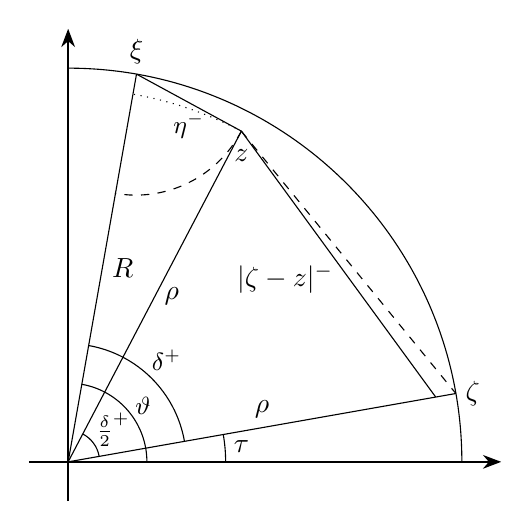
\begin{tikzpicture}
            \coordinate (zeta) at (4.924, 0.868);
            \coordinate (z) at (2.2, 4.2);
            \coordinate (xi) at (0.868, 4.924);
            \coordinate (auxiliary1) at ($(0,0)!0.948!(zeta)$);

            \draw[-{Stealth}, thick] (-0.5, 0) -- (5.5, 0);
            \draw[-{Stealth}, thick] (0, -0.5) -- (0, 5.5);
            \draw[thin] (5,0) arc[start angle=0, end angle=90, radius=5];
            \draw[thin] (0, 0) -- (zeta);
            \draw[thin] (0, 0) -- (xi);
            \draw[thin] (0, 0) -- (z);
            \draw[thin] (z) -- (xi);
            \draw[thin] (z) -- (auxiliary1);
            \draw[dashed, thin] (z) -- (zeta);
            \draw[thin] ($(0,0)!0.08!(zeta)$) arc[start angle=10, end angle=62.35, radius=0.4];
            \draw[thin] ($(0,0)!0.3!(zeta)$) arc[start angle=10, end angle=80, radius=1.5];
            \draw[thin] (2,0) arc[start angle=0, end angle=10, radius=2];
            \draw[thin] (1,0) arc[start angle=0, end angle=80, radius=1];
            \draw[dashed] (z) arc[start angle=-27.65, end angle=-100, radius=1.516];
            \draw[dotted] (z) arc[start angle=62.35, end angle=80, radius=4.741];

            \node[anchor=west] at (zeta) {\(\zeta\)};
            \node[anchor=north] at ([yshift=-3pt] z) {\(z\)};
            \node[anchor=south] at (xi) {\(\xi\)};
            \node[anchor=south] at ($(0,0)!0.5!(zeta)$) {\(\rho\)};
            \node[anchor=north] at ($(z)!0.5!(xi)$) {\small\(\eta^-\)};
            \node[anchor=west] at ($(0,0)!0.5!(xi)$) {\(R\)};
            \node[anchor=west] at ($(z)!0.5!(0,0)$) {\(\rho\)};
            \node[anchor=north] at (0.57,0.75) {\small \(\tfrac{\delta}{2}^+\)};
            \node[anchor=north] at (0.95,0.95) {\small\(\vartheta\)};
            \node[anchor=north] at (1.25,1.55) {\small\(\delta^+\)};
            \node[anchor=north] at (2.2,0.4) {\(\tau\)};
            \node[anchor=east] at ([yshift=-6pt, xshift=-2pt] $(z)!0.5!(zeta)$) {\(|\zeta-z|^-\)};
        \end{tikzpicture}
        \caption{\(\zeta\), \(\xi\), and \(z\) when \(\abs{\vartheta-\tau}>\delta\), with angles and distances marked. The use of \(+\) and \(-\) denote a value more or less (respectively) than the proceeding value.}
        \label{fig:dirichletproblemwithlaplaceequationsolution_secondintegral}
    \end{figure}Since \(\varphi\) is continuous on a compact set \(\partial D(0,R)\), it is bounded by \autoref{thm:heinecantor}, or \(M=\sup_{\qty|\zeta|=R}\abs{\varphi(\zeta)}\) is finite. The Poisson kernel can be rewritten as \[P(\zeta,z)=\frac{R^2-\rho^2}{2\piup\qty|\zeta-z|^2},\]
    where \(\zeta=R\ee^{\ii\tau}\) and \(z=\rho \ee^{\ii\theta}\), with \(\abs{\vartheta-\tau}>\delta\). Then \(\exists\eta>0\) such that \(\forall z\) with \(|\xi-z|<\eta\),
    \begin{equation}
        \abs{\theta-\tau}>\frac{\delta}{2}\label{eq:dirichletproblemwithlaplaceequationsolution_constraint1},
    \end{equation} and
    \begin{equation}
        \rho>\frac{R}{2}\Longrightarrow\eta\leq\frac{R}{2}\label{eq:dirichletproblemwithlaplaceequationsolution_constraint2}
    \end{equation} (these can be arbitrarily chosen for different resulting bounds) as in \autoref{fig:dirichletproblemwithlaplaceequationsolution_secondintegral}. Then, \[|\zeta-z|^2>4\rho^2\sin[2](\frac{\delta}{4})>\frac{1}{2}R^2\qty(1-\cos(\frac{\delta}{2})).\]

    We aim to prove that \(\abs{I_2}<\varepsilon\). Since \(\abs{\varphi\qty(R\ee^{\ii\vartheta})-\varphi(\zeta)}<2M\), the condition is satisfied if \(\int_{\abs{\vartheta-\tau}>\delta}\frac{R^2-\rho^2}{\piup R^2\qty(1-\cos(\frac{\delta}{2}))}\dd{\tau}<2\frac{R^2-\rho^2}{R^2\qty(1-\cos(\frac{\delta}{2}))}< \frac{\varepsilon}{2M}\), and from rearrangement, we can tighten the constraint with:
    \begin{equation}
        R^2-\rho^2<\frac{\varepsilon}{4M}R^2\paren{1-\cos(\frac{\delta}{2})}\Longleftarrow R-\rho<\frac{\varepsilon}{8M}R\paren{1-\cos(\frac{\delta}{2})}.\label{eq:dirichletproblemwithlaplaceequationsolution_constraint3}
    \end{equation}
    From \autoref{fig:dirichletproblemwithlaplaceequationsolution_secondintegral}, it is evident that \(R-\rho<|\xi-z|<\eta\). In order for equation~\eqref{eq:dirichletproblemwithlaplaceequationsolution_constraint1} to be true, we can enforce that \(\abs{\vartheta-\theta}<\frac{\delta}{2}\). In other words \(\abs{\xi-z}^2<R^2+\rho^2-2R\rho\cos(\frac{\delta}{2})\).

    Obviously, this is satisfied if \(|\xi-z|^2<\frac{R^2}{2}\paren{1-\cos(\frac{\delta}{2})}<2\rho^2\qty(1-\cos(\frac{\delta}{2}))\). This can be rearranged into \(|\xi-z|<\frac{R\sqrt{2}}{2}\sqrt{1-\cos(\frac{\delta}{2})}=R\sin\qty(\frac{\delta}{4})\). Therefore, we can choose \[\eta=\min\qty[\frac{\varepsilon}{8M}R\paren{1-\cos(\frac{\delta}{2})},R\sin\qty(\frac{\delta}{4}),\frac{R}{2}]>0,\] under which equations \eqref{eq:dirichletproblemwithlaplaceequationsolution_constraint1}, \eqref{eq:dirichletproblemwithlaplaceequationsolution_constraint2} and \eqref{eq:dirichletproblemwithlaplaceequationsolution_constraint3} are satisfied.

    Hence, \(\forall\varepsilon>0\), \(\exists\eta>0\) such that \(\forall z\) with \(0<\abs{\xi-z}<\eta\), we have \(\abs{\varphi(\xi)-u(z)}<2\varepsilon\). Then equation~\eqref{eq:dirichletproblemwithlaplaceequationsolution_limittoboundary} follows.

    We will now show that \(u(z)\) is unique. Assume that \(v\not\equiv u\) on \(\overline{D(0,R)}\) also solves the problem. Then \(u-v\) is harmonic and vanishes on \(\partial D(0,R)\). By the Poisson Integral Formula (equation~\eqref{eq:poissonintegralformula2}), \(u(z)-v(z)=\int_0^{2\piup}P(\zeta,z)\qty[u(\zeta)-v(\zeta)]\dd{\tau}=0\) for all \(z\in D(0,R)\). Since \(u-v\) vanishes, we have a contradiction.
\end{proof}
\subsubsection{In Harmonic Analysis}
Consider \(R=1\), \(\zeta=\ee^{\ii\tau}\), and \(z=\rho \ee^{\ii\theta}\) in equation~\eqref{eq:poissonintegralformula2}:
\begin{gather}
    u(z)=\frac{1}{2\piup}\int_0^{2\piup} u(\zeta)\frac{1-|z|^2}{\abs{\zeta-z}^2}\dd{\tau} = \frac{1}{2\piup}\int_0^{2\piup}\frac{\qty(1-\rho^2)u\qty(\ee^{\ii\tau})\dd{\tau}}{\qty(\ee^{\ii\tau}-\rho \ee^{\ii\theta})\qty(\ee^{-\ii\tau}-\rho \ee^{-\ii\theta})} \nonumber \\
    =\frac{1}{2\piup}\int_0^{2\piup} \frac{\qty(1-\rho^2)u\qty(\ee^{\ii\tau})\dd{\tau}}{1+\rho^2-2\rho\cos(\theta-\tau)}.\label{eq:poissonintegralformulatrigonometricsubstitution}
\end{gather}
Since \(u\qty(z)\) is continuous on \(\partial\mathbb{D}\) and \(u\circ\exp(\ii\theta)\) is periodic with period \(2\piup\), it admits a Fourier series representation
\begin{equation}
    u\qty(\ee^{\ii\theta})\sim\sum_{n=-\infty}^\infty a_n \ee^{\ii n\theta},\qquad a_n=\frac{1}{2\piup}\int_0^{2\piup} u\qty(\ee^{\ii\tau})\ee^{-\ii n\tau}\dd{\tau}. \label{eq:poissonintegralformulafourierseries}
\end{equation}
This series may diverge. Observe that continuity of \(u\) on the compact set \(\partial\mathbb{D}\) implies uniform boundedness: \(\exists M>0\) such that \(\abs{u\qty(\ee^{\ii\theta})} \leq M\) for all \(\theta\) (\autoref{thm:continuousfunctionboundedoncompact}). Consequently, \(\abs{a_n} \leq M\). Introducing factors \(\rho^{\abs{n}}\) with \(\abs{\rho}<1\) yields a convergent series:
\[\sum_{n=-\infty}^\infty a_n \ee^{\ii n\theta}\rho^{\abs{n}}, \quad\abs{\sum_{n=-\infty}^\infty a_n \ee^{\ii n\theta}\rho^{\abs{n}}}\leq\sum_{n=-\infty}^\infty\abs{a_n}\rho^{\abs{n}}\leq M \frac{1+\abs{\rho}}{1-\abs{\rho}}.\]
Substituting the coefficients gives
\begin{align*}
    \sum_{n=-\infty}^\infty a_n \ee^{\ii n\theta}\rho^{\abs{n}} & =\sum_{n=-\infty}^\infty \qty(\frac{1}{2\piup}\int_0^{2\piup}u\qty(\ee^{\ii\tau})\ee^{-\ii n\tau}\dd{\tau}) \ee^{\ii n\theta}\rho^{\abs{n}} \\
    & =\frac{1}{2\piup} \sum_{n=-\infty}^\infty \int_0^{2\piup}\rho^{\abs{n}} u\qty(\ee^{\ii\tau}) \ee^{\ii n(\theta-\tau)}\dd{\tau}.
\end{align*}
By the Weierstrass \(M\)-Test (\autoref{thm:weierstrassmtest}) and \autoref{thm:limitintegralswitch},
\begin{equation}
    \frac{1}{2\piup}\sum_{n=-\infty}^\infty \int_0^{2\piup} \rho^{\abs{n}}u\qty(\ee^{\ii\tau}) \ee^{\ii n(\theta-\tau)} \dd{\tau}=\frac{1}{2\piup} \int_0^{2\piup} u\qty(\ee^{\ii\tau})\sum_{n=-\infty}^\infty \rho^{\abs{n}} \ee^{\ii n(\theta-\tau)}\dd{\tau}.\label{eq:poissonintegralformulafourierseriespostintegralsummationswitch}
\end{equation}
The summation simplifies as follows:
\begin{align*}
    \sum_{n=-\infty}^\infty \rho^{\abs{n}} \ee^{\ii n(\theta-\tau)} & =\sum_{n=0}^\infty \rho^n \ee^{\ii n(\theta-\tau)}+\sum_{n=1}^\infty \rho^n \ee^{-\ii n(\theta-\tau)} \\
    & =1+2\sum_{n=1}^\infty\rho^n\cos[n(\theta-\tau)]                                                    \\
    & =1+2\Re\sum_{n=1}^\infty\rho^n \ee^{\ii n(\theta-\tau)}                                            \\
    & =1+2\Re\qty[\frac{\rho \ee^{\ii(\theta-\tau)}}{1-\rho \ee^{\ii(\theta-\tau)}}]                     \\
    & =\frac{1-\rho^2}{1+\rho^2-2\rho\cos(\theta-\tau)}.
\end{align*}
Substituting into \eqref{eq:poissonintegralformulafourierseriespostintegralsummationswitch} yields
\[\sum_{n=-\infty}^\infty a_n \ee^{\ii n\theta}\rho^{\abs{n}}=\frac{1}{2\piup}\int_0^{2\piup}\frac{\qty(1-\rho^2)u\qty(\ee^{\ii\tau})}{1+\rho^2-2\rho\cos(\theta-\tau)}\dd{\tau}=u\qty(\rho \ee^{\ii\theta}).\]
Furthermore, by the proof of \autoref{thm:dirichletproblemwithlaplaceequationsolution} (specifically equation~\eqref{eq:dirichletproblemwithlaplaceequationsolution_limittoboundary}),
\[\lim_{\rho\to1^-}\sum_{n=-\infty}^\infty a_n \ee^{\ii n\theta}\rho^{\abs{n}}=u\qty(\ee^{\ii\theta}).\]
Thus, for any continuous function \(u\) on \(\partial\mathbb{D}\), its Fourier series is \textit{Abel summable} to \(u\).

We now establish that real-valued continuous functions satisfying the mean-value property are harmonic.
\begin{theorem}\label{thm:meanvaluepropertysolutionsareharmonic}
    Let \(U\subseteq\mathbb{C}\) be open and \(f:U\to\mathbb{R}\) continuous. Suppose for every \(z_0\in U\), there exists \(\lambda>0\) with \(\overline{D\qty(z_0,\lambda)}\subseteq U\) such that for all \(0<\varepsilon\leq\lambda\),
    \[f(z_0)=\frac{1}{2\piup}\int_0^{2\piup} f\qty(z_0+\varepsilon \ee^{\ii t})\dd{t}.\]
    Then \(f\) is harmonic on \(U\).
\end{theorem}
\begin{proof}
    Fix \(z_0\in U\) arbitarily and choose \(\lambda>0\) such that \(\overline{D\qty(z_0,\lambda)}\subset U\). Because \(f\in C^0\qty(\partial D\qty(z_0,\lambda))\), \autoref{thm:dirichletproblemwithlaplaceequationsolution} guarantees the existence of a unique harmonic function \(u\) on \(D\qty(z_0,\lambda)\) satisfying
    \[u(z)=\int_0^{2\piup}f(\zeta)P\qty(\zeta,z) \dd{\tau},\]
    with \(u=f\) on \(\partial D\qty(z_0,\lambda)\). Define \(\psi=f-u\) on \(\overline{D\qty(z_0,\lambda)}\). Then \(\psi\) is continuous, satisfies the mean-value property, and vanishes on \(\partial D\qty(z_0,\lambda)\). By the proof of \autoref{thm:maximummodulus}, which relies solely on the mean-value property, \(\psi\equiv 0\) on \(\overline{D\qty(z_0,\lambda)}\). Thus \(f\equiv u\) on \(\overline{D\qty(z_0,\lambda)}\), implying \(f\) is harmonic at \(z_0\). The arbitrariness of \(z_0\) establishes harmonicity on \(U\).
\end{proof}
\section{The Theory of Weierstrass}
While Weierstrass' contributions in complex analysis are mainly characterized by his discoveries on uniform convergence, he also characterized entire and \textit{meromorphic functions} and a unique representation of entire functions, as well as his contributions toward the study of \textit{essential singularities}.

To help understand the behavior of non-removable singularities, we will introduce the concept of \textit{Laurent series}.
\subsection{Laurent Series}
The Laurent series generalizes the Taylor series to holomorphic functions with isolated singularities. While Taylor series are valid within a disk centered at a point of holomorphy, Laurent series apply to annular regions surrounding a singularity, making them essential for studying functions near non-removable singularities (refer to \autoref{thm:removablesingularitiesriemann}).

We now introduce a fundamental result in complex analysis due to Weierstrass, which formalizes the conditions under which the limit of a sequence of holomorphic functions is itself holomorphic. This theorem not only guarantees the holomorphy of the limit function but also the uniform convergence of its derivatives (its statement was used in the proof of \autoref{thm:hurwitzsimplecase}).
\begin{theorem}[Weierstrass]\label{thm:weierstrassuniformlimit}
    Let \(\cbraces{f_n(z)}_{n\in\mathbb{N}}\) be a sequence of holomorphic functions on an open region \(U\subseteq\mathbb{C}\) that converges uniformly to \(f(z)\) on every compact subset of \(U\). Then \(f(z)\) is holomorphic on \(U\), and \(\forall k\in\mathbb{N}\), the sequence \(\cbraces{f^{(k)}_n(z)}_{n\in\mathbb{N}}\) uniformly converges to \(f^{(k)}(z)\) on all compact subsets of \(U\).
\end{theorem}
\begin{proof}
    By Morera's Theorem (\autoref{thm:morera}) and the uniform convergence of \(\qty{f_n(z)}\), the holomorphy of \(f(z)\) follows (refer to equation~\eqref{eq:hurwitzsimplecase_integrallimitswitchforholomorphy} and preceding explanations).

    Following the same logic, by \autoref{crl:nthderivativeboundedsupremum}, \(\forall k\in\mathbb{N}\) and for all compact \(K\subset U\) and open \(V\supset K\) relatively compact in \(U\) there exists a finite constant \(c_k>0\) such that
    \[\lim_{n\to\infty}\sup_{z\in K}\abs{f_n^{(k)}(z)-f^{(k)}(z)}\leq c_k\lim_{n\to\infty}\sup_{z\in V}\abs{f_n(z)-f(z)}.\] Since \(\cbraces{f_n(z)}\) is uniformly convergent, the limit on the right-hand side vanishes. Then,
    \[\lim_{n\to\infty}\sup_{z\in K}\abs{f_n^{(k)}(z)-f^{(k)}(z)}=0,\] and therefore \(\qty{f^{(k)}_n(z)}\) uniformly converges on all compact subsets of \(U\).
\end{proof}
The condition of uniform convergence on every compact subset can also be significantly loosened, by the fact demonstrated below:
\begin{lemma}
    Let \(U\subseteq\mathbb{C}\) be open and bounded, and let \(\qty{f_n(z)}\) be holomorphic on \(U\). Let \(K\subseteq U\) be compact. If \(f_n\rightrightarrows f\) on \(\partial K\), then \(f_n\rightrightarrows f\) on \(K\).
\end{lemma}
\begin{proof}
    By the converse statement of the Cauchy Criterion (\autoref{thm:cauchycriterionuniformconvergence}), \(\forall\varepsilon>0\), \(\exists N\in\mathbb{N}\) such that \(\forall n,m>N\), \[\sup_{z\in\partial K}\qty|f_n(z)-f_m(z)|<\varepsilon.\]
    By the Maximum Modulus Principle (\autoref{thm:maximummodulus}) on \(f_n-f_m\), \[\sup_{z\in\partial K}\abs{f_n(z)-f_m(z)}=\sup_{z\in K}\abs{f_n(z)-f_m(z)}<\varepsilon.\]
    It follows that \(f_n\rightrightarrows f\) on \(K\) by \autoref{thm:cauchycriterionuniformconvergence}.
\end{proof}
\begin{remark}
    From the above result, the uniform convergence on every compact subset in \autoref{thm:weierstrassuniformlimit} can therefore be loosened to the uniform convergence on every simple closed curve.
\end{remark}
We will now study Laurent series. Let \(a\in\mathbb{C}\) and \(\qty{c_n}_{n\in\mathbb{Z}}\subset\mathbb{C}\) be constants. A series in the form of
\begin{equation}\label{eq:laurentseries}
    f(z)=\sum_{n=-\infty}^\infty c_n(z-a)^n
\end{equation}
is a Laurent series at the point \(a\). The series can be separated into a power series with non-negative exponents,
\begin{equation}
    \varphi(z)=\sum_{n=0}^\infty c_n(z-a)^n,\label{eq:laurentseriesnonnegativeexponents}
\end{equation} and a power series with negative exponents,
\begin{equation}
    \psi(z)=\sum_{n=1}^{\infty}c_{-n}(z-a)^{-n}.\label{eq:laurentseriesnegativeexponents}
\end{equation} Equation~\eqref{eq:laurentseries} is said to be convergent at \(z=z_0\) if the two power series are both convergent. Let the convergence radius of equation~\eqref{eq:laurentseriesnonnegativeexponents} be \(R=\frac{1}{\varlimsup_{n\to\infty}\sqrt[n]{\abs{c_n}}}\) by the Cauchy--Hadamard Theorem (\autoref{thm:cauchyhadamard}). It follows that the \(\varphi\) is holomorphic on \(D(a,R)\). Let \(\zeta=(z-a)^{-1}\). Then equation~\eqref{eq:laurentseriesnegativeexponents} becomes \(\sum_{n=1}^\infty c_{-n}\zeta^n\). This series converges when \(\abs{\zeta}<\frac{1}{\varlimsup_{n\to\infty}\sqrt[n]{\abs{c_{-n}}}}=\lambda\). Let \(r=\frac{1}{\lambda}\). Then \(\psi(z)\) converges when \(\abs{z-a}>\varlimsup_{n\to\infty}\sqrt[n]{\abs{c_{-n}}}\), or when \(z\in\mathbb{C}\setminus\overline{D(a,r)}\).

If \(R>r\), then \(f\) is convergent on the annulus \(D(a,R)\setminus\overline{D(a,r)}\) and divergent on \(\mathbb{C}\setminus\overline{D(a,R)}\cup D(a,r)\). If \(r=R\), the series diverges possibly everywhere but on \(\partial D(a,r)\). Similar to power series with positive exponents, the convergence on the boundary varies. For example, \(\sum_{\substack{n=-\infty\\n\neq0}}^\infty\frac{z^n}{n^2}\), where \(R=r=1\), converges (absolutely) on \(\partial\mathbb{D}\), whereas \(\sum_{n=-\infty}^\infty z^n\) diverges on all of \(\partial\mathbb{D}\), while \(\sum_{\substack{n=-\infty\\n\neq0}}^\infty\frac{z^n}{n}\) converges (conditionally) on all of \(\partial\mathbb{D}\setminus\qty{1}\) and diverges at \(z=1\). If \(r>R\), then the series is divergent on all of \(\mathbb{C}\). The region \(D(a,R)\setminus\overline{D(a,r)}\) is known as the \textit{annulus of convergence}. \(f(z)\) in equation~\eqref{eq:laurentseries} is holomorphic over this annulus. \(\varphi(z)\) is known as the \textit{holomorphic part} of \(f(z)\), and \(\psi(z)\) is known as the \textit{principal part} of the Laurent series. The properties of the convergence disk in Abel's Theorem (\autoref{thm:abelradius}) can be generalized to Laurent series. In other words, \(f\) is absolutely convergent on the annulus and is uniformly convergent on every compact subset of it.
\begin{theorem}\label{thm:laurentexpansionofholomorphicfunction}
    Let \(V=\cbraces{z\in\mathbb{C}}{r<\abs{z-a}<R}\) for some \(0\leq r<R\leq\infty\). Let \(f\) be holomorphic on \(V\). Then \(f\) has the unique \textit{Laurent expansion}
    \begin{equation}
        f(z)=\sum_{n=-\infty}^\infty c_n(z-a)^n\label{eq:laurentexpansionofholomorphicfunction_statement}
    \end{equation} when \(z\in V\), where \(c_n=\frac{1}{2\piup\ii}\oint_{\gamma}\frac{f(\zeta)\ddzeta}{(\zeta-a)^{n+1}}\), where \(\gamma\subset V\) is a simple closed curve enclosing \(a\).
\end{theorem}
\begin{proof}
    \begin{figure}
        \centering
        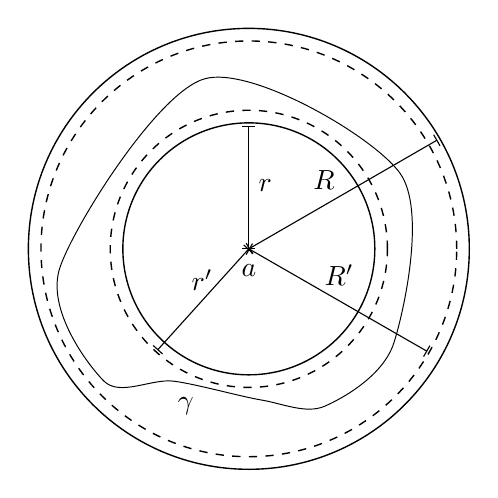
\begin{tikzpicture}\draw[line width=0.35] plot[smooth cycle] coordinates {
                (-2.4,-0.24) (-1.84,-1.68) (-0.96,-1.68) (0.16,-1.92) (0.96,-2.0) (1.84,-1.2) (1.92,0.96) (-0.56,2.16)
            };
            \draw[line width=0.5] (2.8,0) arc[start angle=0, end angle=360, radius=2.8];
            \draw[line width=0.5, dashed] (2.64,0) arc[start angle=0, end angle=360, radius=2.64];
            \draw[line width=0.5] (1.6,0) arc[start angle=0, end angle=360, radius=1.6];
            \draw[line width=0.5, dashed] (1.76,0) arc[start angle=0, end angle=360, radius=1.76];
            \draw[thin, |-|, line cap=round, shorten >=1pt] (0,0) -- (2.424,1.4) node[midway, anchor=south east, yshift=-2pt] {\(R\)};
            \draw[thin, |-|, line cap=round, shorten >=1pt] (0,0) -- (0,1.6) node[midway, right] {\(r\)};
            \draw[thin, |-|, line cap=round, shorten >=1pt] (0,0) -- (2.296,-1.32) node[midway, anchor=south, yshift=2pt] {\(R'\)};
            \draw[thin, |-|, line cap=round, shorten >=1pt] (0,0) -- (-1.184,-1.312) node[midway, anchor=south] {\(r'\)};

            \node[anchor=north] at (0,-0.08) {\(a\)};
            \node[anchor=north] at (-0.8,-1.76) {\(\gamma\)};
        \end{tikzpicture}
        \caption{The annulus \(V\), with \(\gamma_1\), \(\gamma_2\), and \(\gamma\).}
        \label{fig:laurentexpansionofholomorphicfunction}
    \end{figure}By the openness of \(V\), there exist two circles \(\gamma_1\subset V\) with radius \(r'\) and \(\gamma_2\subset V\) with radius \(R'\) centered at \(a\) such that \(\gamma\) encloses \(\gamma_1\) and \(\gamma_2\) encloses \(\gamma\) both without intersection. Let \(W=\cbraces{z\in V}{r'<|z-a|<R'}\) and \(z\in W\) be arbitrary. By the Cauchy--Goursat Formula (\autoref{thm:cauchygoursatformula}), \[f(z)=\frac{1}{2\piup\ii}\qty(\oint_{\gamma_2}\frac{f(\zeta)\ddzeta}{\zeta-z}-\oint_{\gamma_1}\frac{f(\zeta)\ddzeta}{\zeta-z}).\]
    \(\forall\zeta\in\gamma_1\) (or \(|\zeta-a|=r'\)), \(\abs{\zeta-a}<\abs{z-a}\) and therefore, \(\frac{\abs{\zeta-a}}{\abs{z-a}}<1\). It follows that
    \begin{equation}
        \frac{1}{\zeta-z}=-\frac{1}{(z-a)\qty(1-\frac{\zeta-a}{z-a})}=-\sum_{n=0}^\infty\frac{\qty(\zeta-a)^n}{\qty(z-a)^{n+1}}\label{eq:laurentexpansionofholomorphicfunction_kernelexpansioninside}
    \end{equation} is uniformly convergent with respect to \(\zeta\). Similarly, \(\forall\zeta\in\gamma_2\), \(\abs{\zeta-a}>\abs{z-a}\Leftrightarrow\frac{\abs{z-a}}{\abs{\zeta-a}}<1\), and it follows that
    \begin{equation}
        \frac{1}{\zeta-z}=\frac{1}{(\zeta-a)\qty(1-\frac{z-a}{\zeta-a})}=\sum_{n=0}^\infty\frac{\qty(z-a)^n}{\qty(\zeta-a)^{n+1}}\label{eq:laurentexpansionofholomorphicfunction_kernelexpansionoutside}
    \end{equation} is uniformly convergent with respect to \(\zeta\). By the boundedness of \(f\) on \(\gamma_1\) and \(\gamma_2\) from holomorphy on a compact set, and from the Weierstrass \(M\)--Test (\autoref{thm:weierstrassmtest}), we get that
    \begin{equation}
        f(z)=\frac{1}{2\piup\ii}\qty(\sum_{n=0}^\infty\oint_{\gamma_2}\frac{(z-a)^n}{(\zeta-a)^{n+1}}f(\zeta)\ddzeta+\sum_{n=1}^\infty\oint_{\gamma_1}\frac{(\zeta-a)^{n-1}}{(z-a)^{n}}f(\zeta)\ddzeta).\label{eq:laurentexpansionofholomorphicfunction_finalstep}
    \end{equation}
    By the Cauchy--Goursat Theorem (\autoref{thm:cauchygoursattheorem}), for a given \(n\), \[\int_{\gamma_2^+\cup\gamma^-}\frac{f(\zeta)\ddzeta}{(\zeta-a)^n}=0\qand\int_{\gamma^+\cup\gamma_1^-}f(\zeta)(\zeta-a)^n\ddzeta=0.\]
    In other words, the integrals in equation~\eqref{eq:laurentexpansionofholomorphicfunction_finalstep} are the same as on \(\gamma\). Hence, we get that \[f(z)=\sum_{n=0}^\infty c_n(z-a)^n+\sum_{n=1}^\infty c_{-n}(z-a)^{-n}=\sum_{n=-\infty}^\infty c_n(z-a)^n.\]
    The constants \(\qty{c_n}_{n\in\mathbb{Z}}\) are also unique in the expansion. For the sake of contradiction, assume there exists another set of constants \(\qty{c'_n}_{n\in\mathbb{Z}}\) such that
    \begin{equation}
        f(z)=\sum_{n=-\infty}^\infty c'_n(z-a)^n,\label{eq:laurentexpansionofholomorphicfunction_uniquenessstatement}
    \end{equation}
    where \(z\in V\) and the series is uniformly convergent on \(\gamma\). Let \(m\in\mathbb{Z}\) be arbitrary. By the Cauchy--Goursat Differentiation Formula (\autoref{thm:cauchydifferentiationformula}), \[\int_{\gamma}(z-a)^k\ddz=
        \begin{cases}
            0                      & k\geq0   \\
            2\piup\ii\dv[-k-1]{z}(1) & k\leq -1
        \end{cases}=
        \begin{cases}
            0       & k\neq-1 \\
            2\piup\ii & k=-1    \\
    \end{cases}.\]
    Multiplying equation~\eqref{eq:laurentexpansionofholomorphicfunction_uniquenessstatement} by \((z-a)^{-m-1}\) and from integrating over \(\gamma\), we get that \[\oint_\gamma\frac{f(z)\ddz}{(z-a)^{m+1}}=\oint_{\gamma}\sum_{n=-\infty}^\infty c'_n(z-a)^{n-m-1}\ddz,\] implying that \[2\piup \ii c_m=\sum_{n=-\infty}^\infty c'_n\oint_{\gamma}(z-a)^{n-m-1}\ddz=2\piup\ii c'_m,\]
    which is a contradiction, implying uniqueness.
\end{proof}
\subsection{Isolated Singularities}
An \textit{isolated singularity} of a complex function is a point \(a\in\mathbb{C}\) where a function \(f\) is holomorphic on some open punctured neighborhood of \(a\) (namely, for some \(r>0\), the punctured disk \(D^*(a,r)\)), but not necessarily defined or holomorphic at \(a\) itself. The nature of this isolated singularity is characterized by the principal part \(\psi(z)\) (let \(\varphi(z)\) be the holomorphic part) of the Laurent series of \(f\) at the point \(a\). Specifically, we can analyze the behavior of \(f(z)\) as \(z\to a\).
\begin{enumerate}
    \item\label{itm:isolatedsingularities_removable} If \(\lim_{z\to a}f(z)\) exists and is finite, then \(z=a\) is a removable singularity and can be analytically continued to \(D(a,r)\) by \autoref{thm:removablesingularitiesriemann}. Consequently, \(f(z)\) has a convergent Taylor expansion and the principal part of its Laurent expansion vanishes, and \(f(z)=\varphi(z)\).
    \item\label{itm:isolatedsingularities_pole} If \(\lim_{z\to a}f(z)=\infty\), then \(z=a\) is a \textit{pole} of \(f\) (from the stereographic projection and the Riemann sphere, the \(\infty\) is a single point in \(\extcomplex\), and approaching \(\infty\) does not distinguish between different directions, unlike the use of \(+\infty\) and \(-\infty\)).
        \begin{theorem}\label{thm:isolatedsingularities_pole_laurentexpansion}
            The condition \(\lim_{z\to a}f(z)=\infty\) is equivalent to there being a finite number of nonzero \(c_{-n}\)'s, where \(n\in\mathbb{N}\).
        \end{theorem}
        In other words the principal part of \(f\) is equal to \[\psi(z)=\frac{c_{-1}}{z-a}+\cdots+\frac{c_{-m}}{(z-a)^m}\quad c_{-m}\neq0\] for some \(m\in\mathbb{N}\). Therefore, \(f(z)=\varphi(z)+\psi(z)=\sum_{n=-m}^\infty c_n(z-a)^n=\frac{g(z)}{(z-a)^m}\) on the punctured disk \(D^*(a,r)\), where \(g(z)=\sum_{n=0}^\infty c_{n-m}(z-a)^n\) is holomorphic on \(D(a,r)\) and does not attain a zero at \(z=a\). Then \(f(z)\) has a pole at \(z=a\) with order \(m\). If \(m=1\), the pole is also called a \textit{simple pole}.
        \begin{proof}
            Obviously, under the assumption of a finite, nonempty number of non-negative terms in the principal part of the Laurent expansion coefficients, \(\lim_{z\to a}f(z)\to\infty\). Now we will prove the converse. Let \(g(z)=\frac{1}{f(z)}\). Then \(\lim_{z\to a}g(z)=0\). There exists a \(\delta>0\) such that \(f\) is nonzero on \(D^*(a,\delta)\). Then \(g(z)\) is holomorphic on \(D^*(a,\delta)\) and has a removable singularity at \(z=a\). By \autoref{thm:removablesingularitiesriemann}, \(g\) can be analytically continued to \(D^*(a,\delta)\). Let the multiplicity of the zero at \(z=a\) be \(m\). Then \(g(z)=\phi(z)(z-a)^m\), where \(\phi(z)\) is holomorphic and nonzero at \(z=a\). Then there exists a \(\delta'>0\) such that \(\phi\) is nonzero on \(D(a,\delta')\). It follows that \(\frac{1}{\phi}\) is holomorphic and nonzero on \(D(a,\delta')\). We can then write its Taylor expansion as \[\frac{1}{\phi(z)}=c_{-m}+c_{1-m}(z-a)+\cdots,\]
            where \(c_{-m}\neq0\). It follows that \[f(z)=\frac{1}{g(z)}=\frac{(z-a)^{-m}}{\phi(z)}={c_{-m}}(z-a)^{-m}+c_{1-m}(z-a)^{1-m}+\cdots+c_0+\cdots.\]
            By the uniqueness of the Laurent series (by \autoref{thm:laurentexpansionofholomorphicfunction}), the conclusion follows.
        \end{proof}
    \item\label{itm:isolatedsingularities_essential} If \(\lim_{z\to a}f(z)\) is nonexistent, then \(a\) is known as an \textit{essential singularity}.
        \begin{example}\label{ex:isolatedsingularities_essential_exp1z}
            The function \(\ee^{\frac{1}{z}}\) has an essential singularity at \(z=0\).
        \end{example}
        \begin{proof}
            Observe that \(\lim_{\substack{z\to 0\\z\in\mathbb{R}_{>0}}}=\infty\). Similarly, \(\lim_{\substack{z\to0\\z\in\mathbb{R}_{<0}}}=0\), and \(\lim_{\substack{z\to0\\z\in \ii\mathbb{R}_{>0}}}\) is divergent. Therefore, the limit does not exist.
        \end{proof}
        The implication on its Laurent expansion at \(a\) is:
        \begin{theorem}
            The necessary and sufficient for \(\lim_{z\to a} f(z)\) to not exist is that infinitely many of \(c_{-n}\) (where \(n\in\mathbb{N}\)) are nonzero.
        \end{theorem}
        This follows by elimination from the established trichotomy; if the limit as \(z\to a\) does not exist, then the singularity is neither removable nor a pole (results from \ref{itm:isolatedsingularities_removable} and \ref{itm:isolatedsingularities_pole}). Similar logic can be applied to the coefficients of the Laurent expansion.

        Indeed, in \autoref{ex:isolatedsingularities_essential_exp1z}, the Laurent expansion is equal to:
        \[\ee^{\frac{1}{z}}=\sum_{n=0}^\infty\frac{z^{-n}}{n!},\]
        which has infinitely many nonzero coefficients of negative powers.
\end{enumerate}
A function with an essential singularity exhibits striking behavior. We will first introduce the following famous result.
\begin{theorem}[Casorati--Weierstrass]\label{thm:casoratiweierstrass}
    Let \(a\in\mathbb{C}\) and \(U\subseteq\mathbb{C}\) be open. Suppose \(f:U\setminus\qty{a}\to\mathbb{C}\) is holomorphic with an essential singularity at \(a\). Then the set of values that \(f\) attains on any open punctured neighborhood of \(a\) is dense. In other words, \(\forall\varepsilon,\delta>0\), \(\forall w\in\mathbb{C}\), \(\exists z\in D^*(a,\delta)\) such that \(|f(z)-w|<\varepsilon\).
\end{theorem}
\begin{proof}
    Assume for the sake of contradiction that \(\exists\varepsilon,\delta>0\), and \(\exists w\in\mathbb{C}\) such that \(\forall z\in D^*(a,\delta)\), \(|f(z)-w|>\varepsilon\). Define the auxiliary function \(g(z)=\frac{f(z)-w}{z-a}\), which is holomorphic and non-vanishing on the punctured neighborhood of \(a\). Since as \(z\to a\), \(g(z)\to\infty\), it follows that \(g(z)\) has a pole at \(a\). Let the order of the pole be \(m\in\mathbb{N}\). By \autoref{thm:isolatedsingularities_pole_laurentexpansion}, \(g(z)\) has the Laurent expansion of \[\frac{c_{-m}}{(z-a)^m}+\cdots c_0+c_1(z-a)+\cdots\]
    for some \(m\in\mathbb{N}\). It follows that \[f(z)=\frac{c_{-m}}{(z-a)^{m-1}}+\cdots+c_{-1}+w+c_0(z-a)+\cdots.\] If \(m=1\), then \(f\) has a removable singularity at \(a\). If \(m\geq2\), then \(f\) has a pole at \(a\). Hence, we have a contradiction.
\end{proof}
In \chpref{sec:differentialgeometry}, we will prove a profound generalization of this result (\autoref{thm:greatpicard}), which was first proved by Émile Picard in 1879: \textit{the image of any open punctured neighborhood of an isolated essential singularity of a holomorphic function will attain every value in \(\mathbb{C}\), except for at most one possible exception, infinitely often}.
\subsubsection{At the \texorpdfstring{\(\infty\)}{Infinity} Point}
Given the one-point compactification of \(\mathbb{C}\) into the Riemann sphere \(\extcomplex\), we can now define and analyze the behavior of functions near the point at infinity. Similar to the classification of isolated singularities in \(\mathbb{C}\), we can classify \(\infty\) as a removable singularity, a pole, or an essential singularity of a holomorphic function.

Let \(f:\mathbb{C}\setminus\overline{D(0,R)}\to\mathbb{C}\) be holomorphic for some \(R>0\). Then \(z=\infty\) is an \textit{isolated singularity} of \(f\). To analyze the nature of the singularity, let \(\zeta=\frac{1}{z}\). We define a new function \(g(\zeta)=f\qty(\frac{1}{\zeta})=f(z)\), which is holomorphic on \(D^*\qty(0,\frac{1}{R})\). Then at \(\zeta=0\), \(g(\zeta)\) has the Laurent expansion of \[g(\zeta)=\sum_{n=-\infty}^\infty c_{-n}\zeta^n=\sum_{n=0}^\infty c_{-n}\zeta^n+\sum_{n=1}^\infty c_{n}\zeta^{-n}=\varphi(\zeta)+\psi(\zeta),\]
where \(\varphi\) and \(\psi\) are the holomorphic and principal parts of \(g\), respectively. Let \(\widetilde{\varphi}(z)=\varphi\qty(\frac{1}{z})\), \(\widetilde{\psi}(z)=\psi\qty(\frac{1}{z})\). At \(z=0\), \(f\) then has the Laurent expansion of \[f(z)=\sum_{n=-\infty}^\infty c_nz^n=\sum_{n=0}^\infty c_{-n}z^{-n}+\sum_{n=1}^\infty c_nz^n=\widetilde{\varphi}(z)+\widetilde{\psi}(z).\]

The classification of the singularity at \(\infty\) is then reduced to the classification of the singularity of \(g\) at \(0\):
\begin{enumerate}
    \item If \(z=\infty\) is a removable singularity of \(f(z)\), then \(f(z)\) has the form of \[f(z)=c_0+\frac{c_{-1}}{z}+\frac{c_{-2}}{z^2}+\frac{c_{-3}}{z^3}+\cdots.\]
    \item If \(z=\infty\) is a pole of \(f(z)\) with degree \(m\in\mathbb{N}\), then \(f(z)\) can be written as \[f(z)=c_{m}z^m+c_{m-1}z^{m-1}+\cdots+c_0+\frac{c_{-1}}{z}+\cdots,\] where \(c_{m}\neq0\).
    \item If \(z=\infty\) is an essential singularity of \(f(z)\), then \(f(z)\) can be expanded as \[f(z)=\sum_{n=-\infty}^\infty c_{n}z^n,\]
        where \(\forall N\in\mathbb{N}\), \(\exists n>N\) such that \(c_{n}\neq0\) (infinitely many coefficients of \(\psi\) or \(\widetilde{\psi}\) are nonzero).
\end{enumerate}
\begin{remark}
    Under stereographic projection from the point \(\mqty(0\\0\\1)\) of the unit sphere \(S_2\), a neighborhood of that point maps to a subset of the extended complex plane of the form \(\extcomplex\setminus K\), where \(K\) is a compact and connected subset of \(\mathbb{C}\). Such sets are referred to as \textit{neighborhoods of \(\infty\)} in the Riemann sphere.
\end{remark}
\begin{example}
    The function \(z\mapsto\frac{1}{z}\) has a removable singularity at \(z=\infty\), the function \(z\mapsto z^2\) has a pole at \(z=\infty\), and \(z\mapsto \ee^z\) has an essential singularity at \(z=\infty\).
\end{example}
\subsection{Entireness and Meromorphy}
We have previously defined the concept of an entire function in \chpref{sec:complexdifferentiation}. Let \(f\) be entire with the unique Taylor expansion \(\sum_{n=0}^\infty c_nz^n\). Since \(z=\infty\) is an isolated singularity, by the uniqueness of the Laurent expansion, the expansion at \(z=0\) has the same form as the expansion at \(z=\infty\). We will now analyze the implications on the entire function \(f\) given an isolated singularity.
\begin{enumerate}
    \item If the infinity point is a removable singularity, then \(\lim_{z\to\infty} f(z)\) exists and is finite.
        \begin{lemma}\label{lemma:removablesingularityatinftyentireconstant}
            If \(f(z)\) is entire and has a removable singularity at \(z=\infty\), then \(f\) is constant.
        \end{lemma}
        \begin{proof}
            Let \(z=\frac{1}{\zeta}\), \(g(\zeta)=f\qty(\frac{1}{\zeta})\), which has a removable singularity at \(\zeta=0\). By \autoref{thm:removablesingularitiesriemann}, \(g\) can be analytically continued to all of \(\mathbb{C}\), especially at \(\zeta=0\). Let \(w=g(0)\). Then, \(\forall\varepsilon>0\), \(\exists\delta>0\) such that \(\forall\zeta\in D(0,\delta)\), \(|g(\zeta)-w|<\varepsilon\). It follows that \(\forall |z|>\frac{1}{\delta}\), \(\abs{f(z)}<|w|+\varepsilon\), and is bounded. For the complement, \(\forall z\in \overline{D\qty(0,\frac{1}{\delta})}\), \(f(z)\) is continuous on a compact set, and by \autoref{thm:continuousfunctionboundedoncompact}, is also bounded.

            Then by Liouville's Theorem (\autoref{thm:liouville}), \(f\) is constant.
        \end{proof}
    \item If \(f(z)\) has a pole at \(z=\infty\) of order \(m\in\mathbb{N}\), then \(f\) is a polynomial of degree \(m\).
        \begin{proof}
            By the classification of a pole at \(\infty\), \(f\) can be written as \[f(z)=c_mz^m+c_{m-1}z^{m-1}+\cdots+c_0+\frac{c_{-1}}{z}+\cdots.\]
            Since \(f(z)\) is entire, it is holomorphic at \(z=0\) and has a convergent Taylor expansion. By the uniqueness of Laurent expansions (\autoref{thm:laurentexpansionofholomorphicfunction}), the two expansions are equivalent and therefore all terms with negative exponents vanish, and \[f(z)=c_mz^m+c_{m-1}z^{m-1}+\cdots+c_0,\]
            and since \(c_m\neq0\), the statement is confirmed.
        \end{proof}
    \item If \(f(z)\) has an essential singularity at \(z=\infty\), \(f(z)\) is known as a \textit{transcendental entire function}.
\end{enumerate}
\begin{example}
    The entire functions \(\sin(z)\), \(\cos(z)\), \(\sinh(z)\), \(\cosh(z)\), and \(\exp(z)\) are transcendental.
\end{example}
\begin{definition}[Meromorphic Function]\label{def:meromorphicfunction}
    Let \(U\subseteq\mathbb{C}\) be open, and let \(\cbraces{a_n}_{n\in\mathbb{N}}\subset U\) be a set of isolated points. Suppose \(f:U\setminus\cbraces{a_n}_{n\in\mathbb{N}}\to\mathbb{C}\) is holomorphic and has a pole at each of \(z\in\qty{a_n}\). Then \(f\) is \textit{meromorphic} in \(U\).
\end{definition}
Similar to holomorphy, meromorphy on a compact set can be defined as meromorphy on a neighborhood of the set. In general, we imply for the set to be open unless stated otherwise. If the set is not implicitly specified, we assume meromorphy on \(\mathbb{C}\).

All holomorphic functions are meromorphic functions (with poles on \(\emptyset\)). Consequently, entire functions are meromorphic on \(\mathbb{C}\). All rational functions (including polynomials) are also meromorphic on \(\mathbb{C}\). In the study of meromorphic functions with an isolated singularity at \(\infty\), rational functions are of important interest.

Let \(f(z)\) be rational, written as \(f(z)=\frac{p(z)}{q(z)}\), where \(p\) and \(q\) are polynomials. Let
\begin{gather*}
    p(z)=a_nz^n+a_{n-1}z^{n-1}+\cdots a_0\\
    q(z)=b_mz^m+b_{m-1}z^{m-1}+\cdots b_0,
\end{gather*} where \(a_n,b_m\neq 0\). Trivially, the poles of \(f\) are the zeros of \(q\). Since \[f(z)=\frac{z^n}{z^m}\cdot\frac{a_n+\frac{a_{n-1}}{z}+\cdots+\frac{a_0}{z^n}}{b_m+\frac{b_{m-1}}{z}+\cdots\frac{b_0}{z^m}},\] we have \[\lim_{z\to\infty} f(z)=
    \begin{cases}
        \frac{a_n}{b_m} & n=m \\
        0               & n<m \\
        \infty          & n>m
\end{cases}.\]
We will then introduce the converse:
\begin{theorem}\label{thm:rationalmeromorphicfunctions}
    If \(f(z)\) is meromorphic on \(\mathbb{C}\) and has a pole or removable singularity at \(z=\infty\), then \(f\) is a rational function.
\end{theorem}
\begin{proof}
    Since the singularity at \(\infty\) is isolated, there exists a (punctured) neighborhood of \(\infty\), \(\cbraces{z\in\mathbb{C}}{R<|z|<\infty}\), on which \(f\) is holomorphic. Let \(\psi_\infty(z)\) equal the principal part of \(f(z)\). If \(z=\infty\) is a removable singularity of \(f\), then \(\psi_\infty\) is identically zero, and if \(z=\infty\) is a pole of \(f\), then \(\psi_\infty\) is a polynomial.

    It is clear that \(f\) has finitely many poles in \(\overline{D(0,R)}\). Indeed, if \(f\) has infinitely many poles in the closed disk, by the Bolzano--Weierstrass Theorem (\autoref{thm:bolzanoweierstrass}), the set \[\cbraces{z\in\overline{D(0,R)}}{\lim_{\zeta\to z} f(\zeta)=\infty}\] contains an accumulation point in \(\overline{D(0,R)}\), which is not an isolated singularity, contradicting the definition of meromorphy.

    Let \(z_1,\ldots,z_n\) be the isolated poles of \(f\) in \(\overline{D(0,R)}\). \(\forall k\in\qty{1,2,\ldots,n}\), \(f\) has the Laurent expansion at \(z_k\) with a principal part of \[\psi_k(z)=\frac{c_{k,-1}}{z-z_k}+\frac{c_{k,-2}}{\qty(z-z_k)^2}+\cdots+\frac{c_{k,-m_{k}}}{\qty(z-z_k)^{m_k}}.\] Define the auxiliary function \[\Phi(z)=f(z)-\psi_\infty(z)-\sum_{k=1}^n\psi_k(z),\] which is meromorphic on \(\mathbb{C}\) with singularities at each of \(\qty{z_k}_{k=1}^n\cup\qty{\infty}\). Fix \(j\in\cbraces{1,\ldots n}\). Since \(z_j\) is an isolated singularity, \(\exists\varepsilon_j>0\) such that \(\forall k\neq j\), \(z_k\notin D^*\qty(z_j,\varepsilon_j)\). Then, \(\sum_{\substack{k=1\\k\neq j}}^n \psi_k(z)\) is holomorphic on \(D^*(z_j,\varepsilon_j)\). \(\psi_\infty(z)\) is a polynomial and therefore entire. Lastly, \(f(z)-\psi_j(z)=\varphi_j(z)\) is the holomorphic part of the expansion of \(f(z)\) at \(z_j\), and is holomorphic at \(z_j\). Therefore, \(z=z_j\) is a removable singularity of \(\Phi(z)\). By \autoref{thm:removablesingularitiesriemann}, define \(\Phi(z)\) to be the analytic continuation on all of \(\mathbb{C}\).

    At a neighborhood of \(\infty\), \(f(z)-\psi_\infty(z)\) is the holomorphic part of the expansion of \(f(z)\), consisting of non-positive exponents. Therefore, \(\lim_{z\to\infty} f(z)-\psi_\infty(z)\) is finite. Since \(\psi_k\) are the principal parts of Laurent expansions at finite points, they consist of negative exponents. Therefore, we have \(\lim_{z\to\infty}\sum_{k=1}^n \psi_k(z)=0\), and consequently, \(\Phi(z)\) has a removable singularity at \(\infty\). By \autoref{lemma:removablesingularityatinftyentireconstant}, \(c=\Phi(z)\) is constant.

    Thus, we have \[f(z)=c+\psi_\infty(z)+\sum_{k=1}^n\psi_k(z).\] Since each series contains finitely many terms, \(f(z)\) is rational.
\end{proof}
If \(z=\infty\) is not a pole or removable singularity of a meromorphic function \(f(z)\), then it is either an essential singularity or an accumulation point of poles. In this case, \(f\) is not rational and is known as a \textit{transcendental meromorphic function}.
\subsection{Further Properties of Meromorphic and Entire Functions}
The generalization of \autoref{thm:argumentprincipleholomorphic} is as follows:
\begin{theorem}[Argument Principle]\label{thm:argumentprinciplemeromorphic}
    Let \(U\subseteq\mathbb{C}\) be a region and \(f:U\to\mathbb{C}\) be meromorphic. Let \(\gamma\subset U\) be a simple, closed, positively oriented curve that is null-homotopic in \(U\). If \(f\) has no zeros or poles on \(\gamma\), then \(f\) has finitely many zeros and poles in the region bounded by \(\gamma\), and the number of zeros, \(k\), minus the number of poles, \(k'\), counting multiplicities and orders, is given by
    \[k-k'=\frac{1}{2\piup\ii}\oint_{\gamma}\frac{f'(z)}{f(z)}\ddz.\]
    Let \(\Gamma\) be the image of \(\gamma\) under the map \(w=f(z)\). Then \(k-k'=\frac{1}{2\piup}\Delta_\Gamma\arg(w)\), where \(\Delta_\Gamma\arg(w)\) denotes the total change in argument of \(w\) as it traverses \(\Gamma\).
\end{theorem}
\begin{proof}
    Let \(z_1,\ldots,z_m\) be the distinct zeros of \(f\) enclosed by \(\gamma\) with multiplicities \(k_1,\ldots,k_m\), and \(p_1,\ldots,p_n\) the distinct poles with orders \(k'_1,\ldots,k'_n\). Choose disjoint disks \(D\qty(z_j,\varepsilon_j)\) and \(D\qty(p_j,\varepsilon'_j)\) centered at each zero and pole, contained in \(\mathrm{int}(\gamma)\) and avoiding \(\gamma\). The function \(\frac{f'(z)}{f(z)}\) is holomorphic on \[\mathrm{int}\paren{\gamma}\setminus\paren{\bigcup_{j=1}^m D\qty(z_j,\varepsilon_j)\cup\bigcup_{j=1}^n D\qty(p_j,\varepsilon'_j)}\]
    The oriented boundary is \(\gamma^+\cup\bigcup_{j=1}^m\partial D\paren{z_j,\varepsilon_j}^-\cup\bigcup_{j=1}^n\partial D\paren{p_j,\varepsilon'_j}^-\). By the Cauchy--Goursat Theorem (\autoref{thm:cauchygoursattheorem}),
    \[\oint_{\gamma^+}\frac{f'(z)}{f(z)}\ddz=\sum_{j=1}^m\oint_{\partial D\paren{z_j,\varepsilon_j}^+}\frac{f'(z)}{f(z)}\ddz+\sum_{j=1}^n\oint_{\partial D\paren{p_j,\varepsilon'_j}^+}\frac{f'(z)}{f(z)}\ddz.\]
    Near each zero \(z_j\), write \(f(z)=\paren{z-z_j}^{k_j}h_j(z)\) with \(h_j\) holomorphic and non-vanishing. Then
    \[\frac{f'(z)}{f(z)}=\frac{k_j}{z-z_j}+\frac{h_j'(z)}{h_j(z)}.\]
    Integration yields \(\oint_{\partial D\paren{z_j,\varepsilon_j}}\frac{f'(z)}{f(z)}\ddz=2\piup\ii k_j\) since \(\frac{h_j'}{h_j}\) is holomorphic. Near each pole \(p_j\), write \(f(z)=\paren{z-p_j}^{-k'_j}g_j(z)\) with \(g_j\) holomorphic and non-vanishing. Differentiation gives
    \[\frac{f'(z)}{f(z)}=-\frac{k'_j}{z-p_j}+\frac{g_j'(z)}{g_j(z)}.\]
    Integration yields \(\oint_{\partial D\paren{p_j,\varepsilon'_j}}\frac{f'(z)}{f(z)}\ddz=-2\piup\ii k'_j\). Combining results,
    \[\oint_{\gamma}\frac{f'(z)}{f(z)}\ddz=\sum_{j=1}^m2\piup \ii k_j+\sum_{j=1}^n\qty(-2\piup\ii k'_j)=2\piup\ii\paren{\sum_{j=1}^m k_j-\sum_{j=1}^n k'_j}=2\piup\ii\qty(k-k').\]
    Parametrize \(\Gamma\) by \(w=f(z)\). Then \(\dd{w}=f'(z)\ddz\), and
    \[k-k'=\frac{1}{2\piup\ii}\oint_{\Gamma}\frac{\dd{w}}{w}=\frac{1}{2\piup\ii}\Delta_\Gamma\log(w)=\frac{1}{2\piup}\Delta_\Gamma\arg(w),\]
    completing the proof.
\end{proof}
\subsubsection{The Group of Holomorphic Automorphisms on \texorpdfstring{\(\mathbb{C}\)}{the complex plane}}
In complex analysis, three main sets of interest are \(\mathbb{D}\), \(\mathbb{C}\), and \(\extcomplex\). We will now find \(\Aut(\mathbb{C})\).
\begin{theorem}[The Holomorphic Automorphism Group on \(\mathbb{C}\)]\label{thm:holomorphicautomorphismgrouponcomplexplane}
    \(\forall f\in \Aut(\mathbb{C})\), \(f\) is linear and non-constant. In other words, \(\exists a\in\mathbb{C}^*=\mathbb{C}\setminus\qty{0}\) and \(\exists b\in\mathbb{C}\) such that \[f(z)=az+b.\]
\end{theorem}
\begin{proof}
    First, assume that \(\infty\) is not an essential singularity of \(f(z)\) (we will prove this later). Then \(\infty\) must be a pole by trichotomy, as a removable singularity implies boundedness (\autoref{lemma:removablesingularityatinftyentireconstant}). Therefore, \(f(z)\) is a polynomial of degree \(m\), where \(m\in\mathbb{N}\).

    Since \(f^{-1}\in\Aut(\mathbb{C})\), it is true that \(\qty(f^{-1})'\) is entire. Since \(\qty(f^{-1})'=\frac{1}{f'\qty(f^{-1})}\), it follows that \(f'\) has no zeros in \(\mathbb{C}\). By the Fundamental Theorem of Algebra (\autoref{thm:fundamentaltheoremofalgebra}), if \(m>1\), then \(f'\) has a complex zero, which is a contradiction. Hence, \(f\) must be linear, and all functions in \(\Aut(\mathbb{C})\) are in the form of \(az+b\), where \(a\in\mathbb{C}^*\), \(b\in\mathbb{C}\) are constants. In other words, any holomorphic automorphism on \(\mathbb{C}\) is a composition of a rotation, a dilation, and a translation.

    We will now prove the primary assumption; the singularity at \(z=\infty\) cannot be an essential singularity of \(f(z)\). Let \(w\in\mathbb{C}\) be arbitrary. Then by the Casorati--Weierstrass Theorem (\autoref{thm:casoratiweierstrass}), \(\forall\varepsilon>0\), \(\forall R>0\), \(\exists |z|>R\) such that \(|f(z)-w|<\varepsilon\). Equivalently, \(\forall R>0\), \(\exists\zeta\in D(w,\varepsilon)\) such that \(\abs{f^{-1}(\zeta)}>R\). Since \(f^{-1}\) is continuous on \(\overline{D(w,\varepsilon)}\) by holomorphy, by \autoref{thm:continuousfunctionboundedoncompact}, it is bounded, which is a contradiction.
\end{proof}
\subsubsection{The Group of Meromorphic Automorphisms on \texorpdfstring{\(\extcomplex\)}{the Extended Complex Plane}}
It is generally common to consider a meromorphic function as a function in the form of \(f:U\to\extcomplex\). Let \(\Aut\qty(\extcomplex)\) denote the group of meromorphic automorphisms on \(\extcomplex\).

To make more profound conclusions on the structure of \(\Aut\qty(\extcomplex)\), we will introduce certain concepts from group theory.
\begin{definition}[Coset]\label{def:coset}
    Let \(G\) be a group, and let \(H\leq G\) be a subgroup (operation denoted by juxtaposition). Then the \textit{left coset} of \(H\) in \(G\) with respect to \(g\in G\) is defined as \[gH=\cbraces{gh}{h\in H}.\] The \textit{right coset} is defined as \[Hg=\cbraces{hg}{h\in H}.\] The subgroup \(H\) is \textit{normal} if and only if the left and right cosets are equal. The notation \(H\trianglelefteq G\) is used to represent a normal subgroup. Cosets, like groups and sets, are unordered.
\end{definition}
\begin{definition}[Quotient Group]\label{def:quotientgroup}
    Let \(G\) be a group, and let \(H\trianglelefteq G\) be a normal subgroup. Then the \textit{quotient group} of \(G\) by \(H\) is defined as \[G/H=\cbraces{gH}{g\in G}.\] The operation on the quotient group is defined as \((g_1H)(g_2H)=g_1g_2H\), where \(g_1,g_2\in G\) and \(g_1H,g_2H\in G/H\).
\end{definition}
The normality of \(H\) implies the existence of the quotient group. To see why, let \(g_1,g_1'\in G\) form the same left coset (\(g_1H=g_1'H\)), and let \(g_2,g_2'\in G\) satisfy \(g_2H=g_2'H\). We must ensure that
\begin{equation*}
    (g_1H)(g_2H)=(g_1'H)(g_2'H)\Longleftrightarrow g_1g_2H=g_1'g_2'H.
\end{equation*}
Let \(e\) be the identity element of \(G\) and \(H\). In order for \(g_1H=g_1'H\) to be true, it follows that \(g_1e=g_1\) is mapped to a value in \(g_1'H\). Therefore, \(\exists h_1\in H\) such that \(g_1=g_1'h_1\). Similarly, for some \(h_2\in H\), \(g_2=g_2'h_2\). Hence, \[g_1g_2=g_1'h_1g_2'h_2=g_1'\qty(h_1g_2')h_2.\]
We want to ensure that \(g_1g_2\in g_1'g_2'H\), or equivalently prove that \(g_1'\qty(h_1g_2')h_2\in g_1'g_2'H\). By the uniqueness of inverses, the condition above is equivalent to \(h_1g_2'\in g_2'H
\qty(h_2^{-1})=g_2'H\). Equivalently, \(\exists h_3\in H\) such that \(h_1g_2'=g_2'h_3\). This is satisfied if \(H\) is normal.

Let us now examine \(\Aut\qty(\extcomplex)\). Let \(f(z)\in \Aut\qty(\extcomplex)\) such that \(f(\infty)=\infty\). It follows that \(f\) maps \(\mathbb{C}\) to \(\mathbb{C}\) bijectively and \(f\in\Aut(\mathbb{C})<\Aut\qty(\extcomplex)\). Therefore, \(f(z)\) has the form of \(az+b\), where \(a\in\mathbb{C}^*=\mathbb{C}\setminus\qty{0}\) and \(b\in\mathbb{C}\) are constants.

Let \(f(z)\in\Aut\qty(\extcomplex)\) such that \(f(\infty)\neq\infty\). Then, \(g(z)=\frac{1}{f(z)-f(\infty)}\in\Aut\qty(\extcomplex)\) and \(g(\infty)=\infty\). By the property above, \(g(z)=cz+d\) for some complex \(d\) and nonzero \(c\). Hence, \(f(z)=\frac{f(\infty)(cz+d)+1}{cz+d}\). Let \(a=cf(\infty)\), \(b=df(\infty)+1\), \(f(z)=\frac{az+b}{cz+d}\). Then in this specific construction, \(ad-bc=-c\neq0\). Let the matrix \(\mqty(a&b\\c&d)\) correspond to this transformation, where for any nonzero scalar \(k\), \(k\mqty(a&b\\c&d)\) corresponds to \(\mqty(a&b\\c&d)\). Therefore, we can arbitrarily pick \(ad-bc\) to be \(1\).

Therefore, there exists a one-to-one correspondence between \(\Aut\qty(\extcomplex)\) and the group (under matrix multiplication) of \[\left.\cbraces{\mqty(a&b\\c&d)}{\det\mqty(a&b\\c&d)=1}\middle/\qty{\pm\vb{I}},\right.\]
where \(\vb{I}=\mqty(\imat{2})\). The quotient group (a group of elements in the form \(\qty{\vb{A},-\vb{A}}\)) is taken because the matrix \(\mqty(a&b\\c&d)\) corresponds to the same transformation as \(\mqty(-a&-b\\-c&-d)\). This group, denoted by \(\mathrm{PSL}_2(\mathbb{C})=\left.\mathrm{SL}_2(\mathbb{C})\middle/\qty{\pm \vb{I}}\right.\cong\Aut\qty(\extcomplex)\), is known as the \textit{projective special linear group} of order 2, and is \textit{isomorphic} (one-to-one and homomorphic, or that the operation is preserved, see \autoref{lemma:mobiustransformationcompositionmatrixmultiplication}) to the \textit{group of Möbius transformations}, consisting of all linear fractional transformations.

Therefore, any meromorphic automorphism on \(\extcomplex\) is a composition of rotations, dilations, translations, and inversions. We will now state this formally:
\begin{theorem}[The Meromorphic Automorphism Group on \(\extcomplex\)]\label{thm:meromorphicautomorphismgrouponextendedcomplexplane}
    \(\forall f\in \Aut\qty(\extcomplex)\), \(f\) is a Möbius transformation. In other words, \(\exists a,b,c,d\in\mathbb{C}\) satisfying \(ad-bc\neq 0\) such that \[f(z)=\frac{az+b}{cz+d}.\]
\end{theorem}
The group of holomorphic automorphisms on \(\mathbb{D}\), or \(\Aut(\mathbb{D})\), is also a subgroup of \(\Aut\qty(\extcomplex)\). We have the following property on Möbius transformations:
\begin{lemma}\label{lemma:mobiustransformationcompositionmatrixmultiplication}
    Suppose we have two Möbius transformations represented by the matrices \(\mqty(a&b\\c&d)\) and \(\mqty(e&f\\g&h)\). Then their composition is a Möbius transformation represented by \(\mqty(a&b\\c&d)\mqty(e&f\\g&h)\).
\end{lemma}
\begin{proof}
    From simple substitution, we have
    \begin{align*}
        \frac{a\frac{ez+f}{gz+h}+b}{c\frac{ez+f}{gz+h}+d} & =\frac{aez+af+bgz+bh}{cez+cf+dgz+dh}                \\
        & =\frac{\qty(ae+bg)z+(af+bh)}{\qty(ce+dg)z+(cf+dh)},
    \end{align*}
    which corresponds to the product \(\mqty(a&b\\c&d)\mqty(e&f\\g&h)\).
\end{proof}
We have now introduced three of the most important regions in complex analysis: \(\mathbb{D}\), \(\mathbb{C}\), and \(\extcomplex\). Their importance will be later explained by the Uniformization Theorem (\autoref{thm:uniformization}).
\subsubsection{The Construction of Entire and Meromorphic Functions}
It is common knowledge in algebra that any polynomial can be factored into linear factors. When can this factorization be extended to transcendental entire functions?

We will start by introducing the concept of \textit{infinite products}. Let \(\prod_{k=1}^n\qty(1+u_k)\) be an infinite product. If the limit \(\lim_{n\to\infty}\prod_{k=1}^n\qty(1+u_k)\) exists and is finite, then the infinite product is said to be \textit{convergent}.

For \(x\in\mathbb{R}_{\geq0}\), since \(\ee^x\geq x\) and \(\ee^0=1\), we can integrate over \([0,x]\) to get that \(\ee^x\geq x+1\). Therefore,
\begin{align*}
    \exp(\sum_{k=1}^n\abs{u_k}) & \geq\prod_{k=1}^n \qty(1+\abs{u_k})=1+\sum_{k=1}^n\abs{u_k} \\
    & \quad+\sum_{\substack{j,k\in\qty{1,\ldots,n}                \\j<k}}\abs{u_j u_k}+\cdots+\prod_{k=1}^n\abs{u_k}>\sum_{k=1}^n\abs{u_k}.
\end{align*}
Since the convergence of \(\sum_{k=1}^\infty\qty|u_k|\) is the same as that of \(\exp(\sum_{k=1}^\infty\abs{u_k})\), it follows that the convergence of \(\sum_{k=1}^\infty\abs{u_k}\) is equivalent to that of \(\prod_{k=1}^\infty\qty(1+\abs{u_k})\). If \(\sum_{k=1}^\infty\abs{u_k}\) is convergent, then \(\prod_{k=1}^\infty\qty(1+u_k)\) is \textit{absolutely convergent}. As with the order of summing an absolutely convergent series is unimportant, we may also rearrange terms in an absolutely convergent infinite product.

Similar to series, absolute convergence is a stronger condition than convergence:
\begin{lemma}
    An absolutely convergent infinite product is convergent.
\end{lemma}
\begin{proof}
    Let \(\qty{u_k}_{k\in\mathbb{N}}\) be a complex sequence such that \(\sum_{k=1}^\infty\qty|u_k|\) is convergent. Then \(\prod_{k=1}^\infty\qty(1+u_k)\) is absolutely convergent. Let \(Q_n(z)\) denote the partial products of \(\prod_{k=1}^\infty\qty(1+\abs{u_k})\) and let \(P_n(z)\) denote the partial products of \(\prod_{k=1}^n\qty(1+u_k)\). By the Cauchy Criterion (\autoref{thm:cauchycriterionsequenceconvergence}), we have that \(\forall \varepsilon>0\), \(\exists N\in\mathbb{N}\) such that \(\forall n>m>N\), \(|Q_m(z)-Q_n(z)|<\varepsilon\). Let us now analyze the absolute difference between the \(P_n\) and \(P_m\):
    \begin{align*}
        \abs{P_n-P_m} & =\abs{\prod_{k=1}^n\qty(1+u_k)-\prod_{k=1}^m\qty(1+u_k)}                                 \\
        & =\abs{\prod_{k=1}^{m}\qty(1+u_k)\prod_{k=m+1}^{n}\qty(1+u_k)-\prod_{k=1}^{m}\qty(1+u_k)} \\
        & =\prod_{k=1}^{m}\qty|1+u_k|\cdot\qty|\prod_{k=m+1}^{n}\qty(1+u_k)-1|                     \\
        & \leq\prod_{k=1}^{m}\qty(1+\qty|u_k|)\cdot\qty|\prod_{k=m+1}^{n}\qty(1+\abs{u_k})-1|      \\
        & =\abs{Q_n-Q_m}<\varepsilon,
    \end{align*}
    which therefore satisfies \autoref{thm:cauchycriterionsequenceconvergence}.
\end{proof} We will now provide the following assertions on the \textit{locally uniform convergence} of infinite products:
\begin{lemma}\label{lemma:infiniteproductlocallyuniformconvergencecriterion}
    Let \(U\subseteq\mathbb{C}\) be open and connected. Suppose \(\sum_{k=1}^\infty f_k(z)\) is uniformly convergent on compact subsets of \(U\) such that each \(f_k\) is holomorphic on \(U\). Then the infinite product \(\prod_{k=1}^\infty \exp\qty[f_k(z)]\) is uniformly convergent on compact subsets of \(U\).
\end{lemma}
\begin{proof}
    Let \(K\) be an arbitrary compact subset of \(U\). Since \(\sum_{k=1}^\infty f_k(z)\) converges uniformly on \(K\), it follows that \(\forall\varepsilon>0\), \(\exists N\in\mathbb{N}\) such that \(\forall n>m>N\), \(\abs{\sum_{k=m+1}^n f_k(z)}<\varepsilon\) for all \(z\in K\). Additionally, we have: \[\abs{\prod_{k=1}^n \exp\qty[f_k(z)]-\prod_{k=1}^m\exp\qty[f_k(z)]}=\abs{\exp[\sum_{k=1}^n f_k(z)]-\exp[\sum_{k=1}^m f_k(z)]}.\]
    By \autoref{thm:weierstrassuniformlimit}, the uniform limit \(\sum_{k=1}^\infty f_k(z)\) is holomorphic on \(U\). By continuity and \autoref{thm:continuousfunctionboundedoncompact}, this limit is bounded on \(K\). It follows that each partial sum is uniformly bounded on \(K\). Since the exponential function is Lipschitz continuous on compact subsets of \(\mathbb{C}\), there exists a finite constant \(M>0\) such that \[\abs{\exp[\sum_{k=1}^n f_k(z)]-\exp[\sum_{k=1}^m f_k(z)]}\leq M\abs{\sum_{k=m+1}^n f_k(z)}<M\varepsilon.\]
\end{proof}
\begin{remark}
    Uniform convergence on compact subsets is also known as \textit{compact convergence}. In the case of \(\mathbb{C}\) (or in any topological space such that every point has a compact neighborhood), compact convergence is equivalent to \textit{locally uniform convergence}.
\end{remark}
We also have:
\begin{lemma}\label{lemma:infiniteproductlocallyuniformconvergencecriterion2}
    Let \(U\subseteq\mathbb{C}\) be open and connected. Suppose \(\sum_{k=1}^\infty \abs{f_k(z)}\) is uniformly convergent on compact subsets of \(U\) such that each \(f_k\) is holomorphic on \(U\). Then the infinite product \(\prod_{k=1}^\infty \qty[1+f_k(z)]\) is uniformly convergent on compact subsets of \(U\) to a holomorphic function, which vanishes only at a point \(z\) if and only if \(f_k(z)=-1\) for some \(k\in\mathbb{N}\). The multiplicity at each such zero \(z\) is the sum of the multiplicities of \(1+f_k\) at \(z\) for all \(k\) satisfying \(f_k(z)=-1\).
\end{lemma}
\begin{proof}
    Let \(K\subset U\) be an arbitrary compact set. By the uniform convergence of \(\sum_{k=1}^\infty \abs{f_k(z)}\) on \(K\), it follows that the uniform limit is continuous by the Uniform Limit Theorem (\autoref{thm:uniformlimit}). By continuity on a compact set, it follows that the limit is bounded by some constant \(M'\). Additionally, \(\forall\varepsilon>0\), \(\exists N\in\mathbb{N}\) such that \(\forall n>N\), \(\sum_{k=1}^n \abs{f_k(z)}<M'+\varepsilon\). It follows that the partial sums are uniformly bounded in \(K\) by \(M=\max\qty[\max_{k=1}^N\qty(\max_{z\in K}f_k(z)), M'+\varepsilon]\). Similarly, by earlier discussion of infinite products, we have \[F_n(z)=\prod_{k=1}^n\qty(1+\abs{f_k(z)})\leq\exp\qty(\sum_{k=1}^n\abs{f_k(z)})\leq \ee^{M},\]
    or in other words, the partial products are uniformly bounded on \(K\). Let \(0<\varepsilon<1\) be arbitrary. By definition, there exists \(N\in\mathbb{N}\) such that \(\forall n>m>N\), \(\abs{\sum_{k=m+1}^n f_k(z)}<\varepsilon\) for all \(z\in K\). The difference between the non-absolute partial products satisfies
    \begin{align*}
        \abs{\prod_{k=1}^n\qty(1+{f_k(z)})-\prod_{k=1}^m\qty(1+{f_k(z)})} & \leq \abs{\prod_{k=1}^m\qty(1+{f_k(z)})}\abs{\prod_{k=m+1}^n\qty(1+{f_k(z)})-1} \\
        & \leq\abs{F_m(z)}\abs{\exp\qty(\sum_{k=m+1}^n\abs{f_k(z)})-1}                    \\
        & \leq \ee^M\qty(\ee^\varepsilon -1),
    \end{align*}
    where the second inequality can be easily verified by expanding the product \(\prod_{k=m+1}^n\qty(1+{f_k(z)})-1\) and the triangle inequality.

    Since \(\ee^{\varepsilon}-1\to 0^+\), it follows that \(F(z)=\prod_{k=1}^\infty \qty[1+f_k(z)]\) is uniformly convergent on \(K\). Let \(\xi\in U\) be a point satisfying \(F(\xi)=0\). Since there exists an \(m\in\mathbb{N}\) such that \[\prod_{k=m+1}^\infty \qty(1+f_k(z))\] is non-vanishing at \(z=\xi\), and from the fact that \[F(z)=\prod_{k=1}^m \qty(1+f_k(z))\cdot\prod_{k=m+1}^\infty \qty(1+f_k(z)),\] we can analyze the zeros of the finite product to obtain the conclusion.
\end{proof}
We will now study the construction of an entire function \(f(z)\) via its zeros. We have the following cases:
\begin{enumerate}
    \item If \(f\) has no zeros in \(\mathbb{C}\), then the function defined by \(z\mapsto\frac{f'(z)}{f(z)}\) is entire, it is the derivative of an entire function \(\varphi(z)\). Therefore, the function defined by \(z\mapsto f(z)\ee^{-\varphi(z)}\) has the vanishing derivative \(\dv{z}(f(z)\ee^{-\varphi(z)})=f'(z)\ee^{-\varphi(z)}-\varphi'(z)f(z)\ee^{-\varphi(z)}=0\). It follows that \(f(z)\ee^{-\varphi(z)}\) is constant, and therefore \(f(z)=c\exp(\varphi(z))\) for some constant \(c\in\mathbb{C}\). Since \(\varphi(z)\) is entire, it follows that \(f(z)\) is also entire. Absorb the constant \(c\) into \(\varphi(z)\), and \(f(z)=\exp(\varphi(z))\).\label{itm:entirefunctionconstructednonvanishing}
    \item If \(f\) is entire and has finitely many zeros in \(\mathbb{C}\), namely \(a_0=0,a_1,a_2,\ldots,a_n\) with respective multiplicities \(m_0,m_1,\ldots m_n\) (if \(0\) is not a zero, treat \(m_0=0\)), then at each zero \(a_k\), it has the local Taylor expansion of
        \[f(z)=\sum_{j=m_k}^\infty c_j{\qty(z-a_k)}^{j},\] where \(c_{m_k}\neq 0\). Therefore, we can divide \(f(z)\) by \({\qty(z-a_k)}^j\) to obtain a new entire function with no additional zeros and no zero at \(a_k\). Repeating this for every zero, we can define \(\psi(z)=\frac{f(z)}{p(z)}\), which is entire and has no zeros, where \[p(z)=z^{m_0}{\qty(1-\frac{z}{a_1})}^{m_1}\cdots{\qty(1-\frac{z}{a_n})}^{m_n}.\] We write \(p(z)\) in the above form rather than that of \(z^{m_0}\prod_{k=1}^n{\qty(z-a_k)}^{m_k}\) as we aim to generalize the construction to infinite products to study convergence. By~\ref{itm:entirefunctionconstructednonvanishing}, \(\psi(z)=\exp(\varphi(z))\) for some entire function \(\varphi(z)\). Therefore, we can write
        \begin{equation}
            f(z)=p(z)\exp(\varphi(z)),\label{eq:weierstrassfactorization_finitezeros}
        \end{equation} where \(p(z)\) is a polynomial with zeros at \(a_k\) with respective multiplicities of \(m_k\). The entire functions \(p(z)\) and \(f(z)\) both have the same zeros with matching multiplicities.
    \item If \(f(z)\) is entire and has infinitely many zeros such that \(f\) is not identically zero. It follows that \(f\) has countably many zeros (since the zeros are isolated). Let the zeros be indexed by \(\mathbb{N}\), namely \(a_1,a_2,\ldots\). Without loss of generality, assume that \(\forall n\in\mathbb{N}\), \(0<\abs{a_n}\leq\abs{a_{n+1}}\) (repeated elements representing multiplicities), and \(\lim_{n\to\infty}a_n=\infty\). The case for a zero at \(0\) will be treated differently.

        There exists a positive integer sequence \(p_1,p_2,\ldots\) such that for every positive and finite \(R\), \(\sum_{n=1}^\infty{\qty|\frac{R}{a_n}|}^{p_n+1}\) converges. For example, let \(p_n=n\), and for sufficiently large \(n\), \(\frac{R}{\abs{a_n}}<1\) and the series is convergent. Consider the infinite product
        \begin{equation}
            \prod_{n=1}^\infty{\qty(1-\frac{z}{a_n})}\exp\qty[\frac{z}{a_n}+\frac{1}{2}\qty(\frac{z}{a_n})^2+\cdots+\frac{1}{p_n}{\qty(\frac{z}{a_n})}^{p_n}].\label{eq:infiniteproductweierstrassfactorizationintermediate}
        \end{equation}
        Let
        \begin{gather}
            P_p(z)=z+\frac{1}{2}z^2+\cdots+\frac{1}{p}z^p\nonumber\\
            Q_p(z)=\log(1-z)+P_p(z)\nonumber\\
            E_p(z)=\exp\qty[Q_p(z)]=(1-z)\exp\qty[P_p(z)].\label{eq:weierstrasselementaryfactor}
        \end{gather}
        Therefore, we can rewrite equation~\eqref{eq:infiniteproductweierstrassfactorizationintermediate} as
        \begin{equation*}
            \prod_{n=1}^\infty E_{p_n}\qty(\frac{z}{a_n}).
        \end{equation*}
        The expression in equation~\eqref{eq:weierstrasselementaryfactor} is known as the \(p\)th \textit{Weierstrass elementary factor}.

        By \(\varepsilon\)--\(N\), for a fixed \(R>0\), \(\exists N\in\mathbb{N}\) such that \(\forall n\geq N\), \(\abs{a_n}>2R\) (the coefficient is an arbitrary constant greater than one). Consider the product \(\prod_{n=N}^\infty E_{p_n}\qty(\frac{z}{a_n})\). For \(z\in \overline{D(0,R)}\) and \(n\ge N\), we have \(\qty|\frac{z}{a_n}|\le\frac{1}{2}\). The Taylor expansion \(\log(1-w)=-\sum_{k=1}^\infty\frac{w^k}{k}\) has a convergence disk of \(D(0,1)\). Then,
        \begin{align}
            \abs{Q_{p_n}\qty(\frac{z}{a_n})} & =\abs{-\sum_{k=1}^\infty\frac{1}{k}\qty(\frac{z}{a_n})^k+\sum_{j=1}^{p_n}\frac{1}{k}\qty(\frac{z}{a_n})^k}\leq\sum_{k=p_n+1}^\infty\frac{1}{k}\abs{\frac{z}{a_n}}^k\nonumber                                       \\
            & \leq\sum_{k=p_n+1}^\infty\abs{\frac{z}{a_n}}^k=\abs{\frac{z}{a_n}}^{p_n+1}\frac{1}{1-\abs{\frac{z}{a_n}}}\leq 2\abs{\frac{R}{a_n}}^{p_n+1}(\leq 1).\label{eq:infiniteproductweierstrassfactorizationuniformbound}
        \end{align}
        By the definition of \(\qty{p_n}_{n\in\mathbb{N}}\), the series \(2\sum_{n=1}^\infty\abs{\frac{R}{a_n}}^{p_n+1}\) converges. Therefore, \(\sum_{n=1}^\infty Q_{p_n}\qty(\frac{z}{a_n})\) is uniformly and absolutely convergent on \(\overline{D(0,R)}\) by the Weierstrass \(M\)--Test (\autoref{thm:weierstrassmtest}). We then get that \(\prod_{n=N}^\infty E_{p_n}\qty(\frac{z}{a_n})=\exp(\sum_{n=N}^\infty Q_{p_n}\qty(\frac{z}{a_n}))\) and it uniformly converges on \(\overline{D(0,R)}\) to a nonzero holomorphic function \(f(z)\) on \({D(0,R)}\) by \autoref{lemma:infiniteproductlocallyuniformconvergencecriterion}, \autoref{thm:weierstrassuniformlimit}, and \autoref{thm:hurwitzsimplecase}.

        The zeros of \[\prod_{n=1}^\infty E_{p_n}\qty(\frac{z}{a_n})\] are \(a_1,\ldots, a_{N-1}\) and lie in \(\overline{D(0,2R)}\). To prove the absolute convergence of \(\prod_{n=N}^\infty E_{p_n}\qty(\frac{z}{a_n})\) on \(\overline{D(0,R)}\), we will show that \(\sum_{n=N}^\infty\abs{E_{p_n}\qty(\frac{z}{a_n})-1}\) is convergent. Trivially, when \(\zeta\in\overline{\mathbb{D}}\), we have \(\abs{\exp(\zeta)-1}\leq\exp\qty|\zeta|-1\leq\paren{\ee-1}\abs{\zeta}\). By equation~\eqref{eq:infiniteproductweierstrassfactorizationuniformbound} above, we get that \(\qty|Q_{p_n}\qty(\frac{z}{a_n})|\leq 1\) when \(n\geq N\).

        Therefore, we have
        \begin{align*}
            \abs{E_{p_n}\qty(\frac{z}{a_n})-1} & =\abs{\exp(Q_{p_n}\qty(\frac{z}{a_n}))-1}                                            \\
            & \leq (\ee-1)\abs{Q_{p_n}\qty(\frac{z}{a_n})}\leq2(\ee-1)\abs{\frac{R}{a_n}}^{p_n+1},
        \end{align*}
        which has a convergent series by definition. Therefore, \(\prod_{n=N}^\infty E_{p_n}\qty(\frac{z}{a_n})\) is absolutely convergent on \(\overline{D(0,R)}\).

        Letting \(R\to\infty\), for any such sequence \(\qty{a_n}_{n\in\mathbb{N}}\), we can define the entire function
        \begin{equation}
            f(z)=\prod_{n=1}^\infty E_{p_n}\qty(\frac{z}{a_n})\label{eq:entirefunctionconstructedfrominfinitelymanyzeros}
        \end{equation} to have zeros at each element of the sequence, and for any compact disk \(\overline{D(0,R)}\), the product above is uniformly convergent. We can then formulate:
        \begin{theorem}[Weierstrass Factorization Theorem]\label{thm:weierstrassfactorization}
            Suppose \(f(z)\) is an entire function. Let \(\qty{a_n}_{n\in\mathbb{N}}\) be the sequence of all nonzero zeros of \(f\) satisfying \(a_n\to\infty\) as \(n\to\infty\) and \(0<\qty|a_n|\leq\qty|a_{n+1}|\) (equality of \(a_n\) and \(a_{n+1}\) treated as multiplicities) for all \(n\). Let \(m\) be the multiplicity of \(f(z)\) at \(z=0\) (let \(m=0\) if there is no zero at \(0\)). Then there exists a sequence \(\qty{p_n}_{n\in\mathbb{N}}\) such that \(\forall R>0\), \(\sum_{n=1}^\infty{\qty|\frac{R}{a_n}|}^{p_n+1}\) converges. Then, we can write
            \begin{equation}
                f(z)=z^m\ee^{\varphi(z)}\prod_{n=1}^\infty E_{p_n}\qty(\frac{z}{a_n})\label{eq:weierstrassfactorization_statement}
            \end{equation} on \(D(0,R)\), where \(E_p(z)\) is the \(p\)th Weierstrass elementary factor defined in equation~\eqref{eq:weierstrasselementaryfactor} and \(\varphi(z)\) is an entire function. The infinite product converges uniformly on \(\overline{D(0,R)}\) and converges absolutely on \(\mathbb{C}\). If we let \(p_n=n\), we can write \[f(z)=z^m\ee^{\varphi(z)}\prod_{n=1}^\infty\qty(1-\frac{z}{a_n})\exp\qty[\frac{z}{a_n}+\frac{1}{2}\qty(\frac{z}{a_n})^2+\cdots+\frac{1}{n}\qty(\frac{z}{a_n})^n].\]
        \end{theorem}
        \begin{proof}
            By the argument of equation~\eqref{eq:entirefunctionconstructedfrominfinitelymanyzeros}, construct \(\psi(z)\) to be entire and have zeros at \(\qty{a_n}_{n\in\mathbb{N}}\). Thus, \(z^m\psi(z)\) and \(f(z)\) have the same zeros and corresponding multiplicities. Then the function \(z^m\frac{\psi(z)}{f(z)}\) has removable singularities on all of \(\qty{a_n}_{n\in\mathbb{N}}\cup\qty{0}\) and has an analytic continuation (\autoref{thm:removablesingularitiesriemann}) to an entire and non-vanishing function. Therefore, it can be written as \(z^m\frac{\psi(z)}{f(z)}=\ee^{\phi(z)}\), where \(\phi\). Let \(\varphi=-\phi\), and from rearrangement, we obtain equation~\eqref{eq:weierstrassfactorization_statement}
        \end{proof}
\end{enumerate}
By the construction above, we have:
\begin{corollary}
    Let \(f\) be meromorphic on \(\mathbb{C}\). Then \(f\) can be written as the quotient of two entire functions.
\end{corollary}
\begin{proof}
    Let \(\varphi(z)\) be any entire function with zeros only at each pole of \(f\) (with multiplicities matching the order of each pole). If there are infinitely many poles, we can explicitly construct such a \(\varphi\) by the Weierstrass Factorization Theorem (\autoref{thm:weierstrassfactorization}). If there are finitely many poles, construct \(\varphi\) using equation~\eqref{eq:weierstrassfactorization_finitezeros}. It follows that \(\varphi f\) has can be analytically continued (on its removable singularities) to an entire function \(\phi(z)\) with the same zeros as \(f(z)\). Hence, \[f(z)\varphi(z)=\phi(z)\Longleftrightarrow f(z)=\frac{\phi(z)}{\varphi(z)},\]
    which is an explicit construction.
\end{proof}
Therefore, any meromorphic function on \(\mathbb{C}\) can be expressed as the quotient of two infinite products. Hence, any meromorphic function on \(\mathbb{C}\) can be explicitly written in terms of its zeros and poles.

We will now study the construction of meromorphic functions from their poles and the principal parts of their Laurent expansions at each pole.

Suppose \(n\in\mathbb{N}\) and \(\qty{a_k}_{k=1}^n\subset\mathbb{C}\) is a sequence of distinct values. Let \(\qty{\psi_k(z)}_{k=1}^n\) be a collection of functions in the form of
\begin{equation}
    \psi_k(z)=\sum_{j=m_k}^{p_k}\frac{c_{k,j}}{{\qty(z-a_k)}^j},\label{eq:meromorphicfunctionconstructionprincipalparts}
\end{equation} where \(p_k\geq m_k\) are finite integer constants and \(\qty{c_{k,j}}\) are complex constants.

Suppose that \(f(z)\) is meromorphic on \(\mathbb{C}\) such that \(f\) has finitely many poles. Therefore, \(f\) has an isolated singularity at \(\infty\). We have two cases:
\begin{enumerate}
    \item If \(z=\infty\) is a removable singularity or a pole, by the proof of \autoref{thm:rationalmeromorphicfunctions}, we can construct \(f(z)\) to have poles at each of \(\qty{a_k}_{k=1}^n\) such that the principal parts of \(f\) at each of \(\qty{a_k}_{k=1}^n\) are \(\qty{\psi_k(z)}_{k=1}^n\). It can be explicitly written as \[f(z)=p(z)+\sum_{k=1}^n\psi_k(z)\] (we can absorb the constant \(c\) into the polynomial \(\psi_\infty\) as used in the proof).
    \item In the case that \(f(z)\) is a transcendental meromorphic function with an isolated essential singularity at \(z=\infty\), notice that the function defined by \(\varphi(z)=f(z)-\sum_{k=1}^n\psi_k(z)\) has removable singularities at each of \(\qty{a_k}_{k=1}^n\). Indeed, since the singularities are isolated, for a fixed \(k\), \(\exists\varepsilon_k>0\) such that for any \(j\neq k\), \(a_j\notin D\qty(a_k,\varepsilon_k)\). It follows that \(\psi_j\) is holomorphic on \(D\qty(a_k,\varepsilon_k)\). Notice that \(f(z)-\psi_k\) is the holomorphic part of the Laurent expansion at \(a_k\) and is also holomorphic on the disk. Suppose \(f\) has \(\psi_k\) as the principal part of its Laurent expansion at \(a_k\). Then \(\varphi(z)\) is holomorphic on \(D\qty(a_k,\varepsilon_k)\). Since \(k\) was arbitrarily chosen, \(\varphi\) is entire and transcendental.

        Therefore, \(f\) can be constructed by \[f(z)=\varphi(z)+\sum_{k=1}^\infty\psi_k(z),\]
        for a transcendental entire function \(\varphi(z)\).
    \item The existence of a transcendental meromorphic function \(f\) whose poles have an accumulation point at \(z=\infty\) is the concern of the following theorem:
        \begin{theorem}[Mittag--Leffler]\label{thm:mittagleffler}
            Let \(\qty{a_n}_{n\in\mathbb{N}}\subset\mathbb{C}\) be a sequence of distinct complex numbers such that \(\forall n\in\mathbb{N}\), \(\abs{a_n}\leq\abs{a_{n+1}}\) and \(\lim_{n\to\infty}a_n=\infty\). Let \(\qty{\psi_n}_{n\in\mathbb{N}}\) be a function sequence, each in the form of equation~\eqref{eq:meromorphicfunctionconstructionprincipalparts}. Then,
            \begin{enumerate}[label=(\alph*)]
                \item A meromorphic function \(f(z)\) on \(\mathbb{C}\) can be constructed such that \(\forall n\in\mathbb{N}\), \(f\) has a pole at \(a_n\) with a principal part of \(\psi_n\) at \(a_n\).\label{itm:mittagleffler_existence}
                \item The function \(f(z)\) satisfying the criteria above can be explicitly represented as
                    \begin{equation}
                        f(z)=\varphi(z)+\sum_{n=1}^\infty\qty[\psi_n(z)-p_n(z)]\label{eq:mittagleffler_construction_statement}
                    \end{equation} for some sequence of polynomials \(\qty{p_n(z)}\) and an arbitrary entire function \(\varphi(z)\).\label{itm:mittagleffler_construction}
            \end{enumerate}
        \end{theorem}
        \begin{proof}
            The classical proof for this theorem allows for a more explicit construction, as in equation~\eqref{eq:mittagleffler_construction_statement}. As for the existence, we can prove~\ref{itm:mittagleffler_existence} by using the \(\overline{\partial}\) problem.
            \begin{enumerate}[label=(\alph*)]
                \item Fix \(n\in\mathbb{N}\), let \(U_n\) be an open neighborhood of \(a_n\) such that \(\forall i,j\in\mathbb{N}\) where \(i\neq j\), \(\overline{U_i}\cap \overline{U_j}=\emptyset\). Let \(V_n\) be a neighborhood of \(a_n\) that is relatively compact in \(U_n\). By \autoref{thm:bumpfunctionexistence}, for each \(n\), there is a \(C^\infty\) function \(\varphi_n\) satisfying \[
                        \begin{cases}
                            \varphi_n(z)\equiv 1 & z\in\overline{V_n}          \\
                            \varphi_n(z)\equiv 0 & z\in\mathbb{C}\setminus U_n
                    \end{cases}.\]
                    Let \(u(z)=\sum_{k=1}^\infty\varphi_k(z)\psi_k(z)\), which is an element of \(C^\infty\qty(\mathbb{C}\setminus\qty{a_k}_{k\in\mathbb{N}})\). For a fixed \(n\in\mathbb{N}\), it is true that \(u\equiv\psi_n\) on \(\overline{V_n}\setminus\qty{a_n}\). Hence, although \(u\) is not meromorphic, it does have the required principal part near each \(a_k\). Let \[\phi(z)=
                        \begin{cases}
                            \pdv{u}{\overline{z}} & z\in\mathbb{C}\setminus\qty{a_k}_{k\in\mathbb{N}} \\
                            0                     & z\in\qty{a_k}_{k\in\mathbb{N}}
                    \end{cases}.\]
                    Since \(\pdv{u}{\overline{z}}\equiv\pdv{\psi_n}{\overline{z}}\equiv 0\) and is \(C^\infty\) on \(\overline{V_n}\setminus\qty{a_n}\) and \(\phi\) vanishes on \(\qty{a_k}_{k\in\mathbb{N}}\), \(\phi\in C^\infty(\mathbb{C})\). By the discussion proceeding \autoref{thm:onedimensionalpartialconjugatesolution}, there exists a \(C^\infty\) function \(v(z)\) such that \(\pdv{v}{\overline{z}}=\phi(z)\) on \(\mathbb{C}\). Since \(\phi\) is \(C^\infty\), it follows that \(v\) is also \(C^\infty\). Define \(f(z)=u(z)-v(z)\). Then
                    \[\pdv{f}{\overline{z}} = \pdv{u}{\overline{z}}-\pdv{v}{\overline{z}} = \phi(z)-\phi(z) = 0,\]
                    which implies that \(f\) is holomorphic on \(\mathbb{C} \setminus \qty{a_k}_{k\in\mathbb{N}}\). Since \(u\) has the desired principal part \(\psi_n\) at each \(a_n\) and \(v\) is \(C^\infty\) (and hence removable at each singularity), it follows that \(f\) is meromorphic on \(\mathbb{C}\) with principal parts \(\psi_n\) at each \(a_n\), as desired.
                \item Let \(\qty{\varepsilon_n}_{n\in\mathbb{N}}\) be a positive sequence such that \(\sum_{n=1}^\infty\varepsilon_n\) is convergent. Without loss of generality, let \(a_1=0\) (if \(a_1\) is not a pole, set \(\psi_1=0\)). Choose \(p_1(z)=0\) (this can actually be any arbitrary polynomial). Fix \(n\geq 2\), \(\psi_n\) is a polynomial in terms of \(\frac{1}{z-a_n}\) and has its only pole at \(z=a_n\). Therefore, \(\psi_n(z)\) is holomorphic on \(D\qty(0,\abs{a_n})\) and can be written as \[\psi_n(z)=\sum_{k=0}^\infty \frac{\psi_n^{(k)}(0)}{k!}z^k.\]

                    By \autoref{thm:abelradius}, This series is uniformly convergent on \({D\qty(0,\abs{\frac{a_n}{2}})}\). Hence, \(\exists \lambda_n\in\mathbb{N}\) such that \[\abs{\psi_n(z)-\sum_{k=0}^{\lambda_n} \frac{\psi_n^{(k)}(0)}{k!}z^k}< \varepsilon_n.\] Let \(p_n(z)=\sum_{k=0}^{\lambda_n}\frac{\psi_n^{(k)}(0)}{k!}z^k\). Fix \(R>0\) and let \(N\in\mathbb{N}\) depend on \(R\) such that \(\abs{a_n}>2R\) for all \(n>N\) and \(\abs{a_n}\le 2R\) for all \(n\le N\). Therefore, \(\forall n>N\), \(R<\abs{\frac{a_n}{2}}\). Then \(\forall z\in D(0,R)\), we have \[\abs{\psi_n(z)-p_n(z)}<\varepsilon_n.\]

                    By the convergence of \(\sum_{n=N+1}^\infty\varepsilon_n\), by the Weierstrass \(M\)--Test (\autoref{thm:weierstrassmtest}), the series
                    \begin{equation}
                        \Phi_N(z)=\sum_{n=N+1}^\infty\brackets{\psi_n(z)-p_n(z)}\label{eq:mittagleffler_construction_uniformlyconvergentseries}
                    \end{equation} converges uniformly on \(D(0,R)\). Since \(z<R<\abs{\frac{a_n}{2}}<\abs{a_n}\) when \(n>N\), the pole of \(\psi_n(z)\), \(z=a_n\), is not in \(D(0,R)\) (when \(n>N\)). By \autoref{thm:weierstrassuniformlimit}, equation~\eqref{eq:mittagleffler_construction_uniformlyconvergentseries} is holomorphic on \(D(0,R)\). Let \[\Psi(z)=\sum_{n=1}^N\qty[\psi_n(z)-p_n(z)]+\Phi_N(z).\]
                    The poles of \(\Psi(z)\) in \(D(0,R)\) are all of \(a_n\) with corresponding principal parts \(\psi_n(z)\), where \(n\in\mathbb{N}\) and satisfies \(a_n\in D(0,R)\). Since \(R\) was arbitrarily chosen, \(\Psi\) has poles at each \(a_n\) with the corresponding principal part \(\psi_n(z)\) on \(\mathbb{C}\). Let \(\varphi(z)=f(z)-\Psi(z)\) be analytically continued onto each of \(\qty{a_n}_{n\in\mathbb{N}}\). Then \(\varphi(z)\) is an entire function (since the Laurent expansions of \(\varphi\) at each of \(\qty{a_n}_{n\in\mathbb{N}}\) vanish). By rearrangement, we obtain our desired result.
            \end{enumerate}
        \end{proof}
\end{enumerate}
The Mittag--Leffler Theorem (\autoref{thm:mittagleffler}) can also be generalized as follows:
\begin{theorem}\label{thm:mittaglefflerboundary}
    Let \(U\subset\mathbb{C}\) be an open set with a simple closed boundary \(\partial U\) and let \(E=\qty{a_n}_{n\in\mathbb{N}}\subset U\) be a sequence of distinct complex numbers whose accumulation points lie on \(\partial U\). Let \(\qty{\psi_n}_{n\in\mathbb{N}}\) be a sequence of functions in the form of equation~\eqref{eq:meromorphicfunctionconstructionprincipalparts}. Then there exists a meromorphic function \(f:U\to\mathbb{C}\) with poles at each \(a_n\) with principal parts \(\psi_n\) at each \(a_n\).
\end{theorem}
Indeed, since \(\partial U\cap U=\emptyset\), each \(a_n\) is not an accumulation of \(E\). In other words, for each \(n\in\mathbb{N}\), there exist neighborhoods \(U_n\) of \(a_n\) that are relatively compact in \(U\) with disjoint closures. The proceeding proof is analogous to that of \ref{itm:mittagleffler_existence} in \autoref{thm:mittagleffler}.

Finally, we will examine the construction of entire functions interpolating prescribed values and derivatives at given points.

Let \(\qty{z_j}_{j=1}^n\subset\mathbb{C}\) be a sequence of distinct complex numbers and let \(\qty{w_j}_{j=1}^n\subset\mathbb{C}\) be a sequence of complex numbers. We can then construct a polynomial \(f(z)\) such that \(\forall j\in\qty{1,\ldots,n}\), \(f(z_j)=w_j\). One such explicit formula is given by the \textit{Lagrange interpolation formula}:
\[f(z)=\sum_{j=1}^n\qty[w_j\prod_{\substack{k=1\\k\neq j}}^n\frac{z-z_k}{z_j-z_k}].\]
Then, following the assumption that \(\qty{z_j}_{j=1}^n\subset\mathbb{C}\) is a sequence of distinct complex numbers, let \(\qty{w_{j,k}}_{\substack{j\in\qty{1,\ldots,n}\\ k\in \qty{0,\ldots,n_j}}}\) be a sequence where \(\qty{n_j}_{j=1}^n\subset\mathbb{N}\). Then we can find a polynomial \(f(z)\) such that \(\forall j\in\qty{1,\ldots,n}\), \(\forall k\in\qty{0,\ldots,n_j}\), \(f^{(k)}\qty(z_j)=k!w_{j,k}\) (for clarity's sake, \(j\) selects the pair and \(k\) selects the order of the derivative, whose upper bound varies for each \(j\)). Oftentimes, the factorial coefficient is absorbed into \(\qty{w_{j,k}}\).

As it turns out, an entire function can in fact be constructed for infinitely many interpolation points, or when \(n\to\infty\).
\begin{theorem}\label{thm:generalinterpolationexistence}
    Let \(\qty{z_k}_{k\in\mathbb{N}}\subset\mathbb{C}\) be a discrete set and let \(\qty{w_{k,n}}_{\substack{k\in\mathbb{N}\\n\in\qty{0,\ldots,n_k}}}\) be a sequence where \(\qty{n_k}_{k\in\mathbb{N}}\subset\mathbb{N}\). Then there exists an entire function such that \(\forall k\in\mathbb{N}\), \(\forall n\in\qty{0,\ldots,n_k}\),
    \begin{equation}
        f^{(n)}\qty(z_k)=n!w_{k,n}.\label{eq:generalinterpolationexistence_statement}
    \end{equation}
    In other words, an entire function can be constructed by the given first \(n_k\) coefficients of the Taylor expansion at each each \(z_k\).
\end{theorem}
\begin{proof}
    According to the Weierstrass Factorization Theorem (\autoref{thm:weierstrassfactorization}), we can construct an entire function \(\Phi(z)\) with zeros at each of \(\qty{z_k}_{k\in\mathbb{N}}\) with corresponding multiplicities of \(\qty{n_k}_{k\in\mathbb{N}}\). By the discreteness of \(\qty{z_k}_{k\in\mathbb{N}}\), there exists a corresponding sequence of radii \(\qty{\varepsilon_k}_{k\in\mathbb{N}}\) such that each \(\overline{D\qty(z_k,2\varepsilon_k)}\) are disjoint.

    Define a complex function sequence \(\qty{\phi_k(z)}_{k\in\mathbb{N}}\) with \[\phi_k(z)=\sum_{n=0}^{n_k-1}w_{k,n}\qty(z-z_k)^n,\] where \(k\in\mathbb{N}\). By \autoref{thm:bumpfunctionexistence}, we can construct a \(C^\infty\) sequence of functions \(\qty{\varphi_k(z)}_{k\in\mathbb{N}}\) such that \(\forall k\in\mathbb{N}\), \(\supp\varphi_k\subset D\qty(z_k, 2\varepsilon_k)\), \(\varphi_k\equiv 1\) on \(\overline{D\qty(z_k,\varepsilon_k)}\), and \(0\le\varphi\le 1\) on \(\mathbb{C}\).

    Let \(\Psi\in C^\infty(\mathbb{C})\), and construct
    \begin{equation}
        f(z)=-\Phi(z)\Psi(z)+\sum_{k=1}^\infty\phi_k(z)\varphi_k(z).\label{eq:generalinterpolationexistence_constructionstatement}
    \end{equation}
    Under what conditions on \(\Psi\) will \(f\) be entire? Since the supports of each \(\varphi_k\) are disjoint, the summation \(\sum_{k=1}^\infty\phi_k(z)\varphi_k(z)\) contains at most one nonzero term and is convergent and well-defined. To construct \(f\) to be entire, we must have \(\pdv{f}{\overline{z}}=0\). In other words, we want for \[\pdv{\overline{z}}(\sum_{k=1}^\infty\phi_k\varphi_k)=\pdv{\overline{z}}[\Phi\Psi]\Longleftrightarrow\sum_{k=1}^\infty\phi_k\pdv{\varphi_k}{\overline{z}}=\Phi\pdv{\Psi}{\overline{z}}\] on all of \(\mathbb{C}\). Let \(g(z)=\sum_{k=1}^\infty\phi_k(z)\pdv{\varphi_k(z)}{\overline{z}}\). Since \(\varphi_k\equiv 1\) on \(\overline{D\qty(z_k,\varepsilon_k)}\), \(\pdv{\varphi_k}{\overline{z}}\equiv 0\) on \(\bigcup_{k=1}^\infty \overline{D\qty(z_k,\varepsilon_k)}\). Consequently, \(g(z)\equiv 0\) on \(\bigcup_{k=1}^\infty \overline{D\qty(z_k,\varepsilon_k)}\).

    From rearrangement, we have \(\frac{g(z)}{\Phi(z)}=\pdv{\Psi}{\overline{z}}\), which has removable singularities at each \(z_k\). Define \(\frac{g(z)}{\Phi(z)}=0\) at \(z=z_k\). Under this assertion, we have \(\frac{g(z)}{\Phi(z)}\in C^\infty(\mathbb{C})\). Since the support of \(\frac{g(z)}{\Phi(z)}\) is the union of disjoint compact sets, by \autoref{thm:onedimensionalpartialconjugatesolution}, there exists a function \(\Psi\in C^\infty(\mathbb{C})\) satisfying \(\frac{g(z)}{\Phi(z)}=\pdv{\Psi}{\overline{z}}\). Since \(g\) is vanishing on \(\bigcup_{k=1}^\infty \overline{D\qty(z_k,\varepsilon_k)}\), it follows that \(\frac{g}{\Phi}\) is vanishing on \(\bigcup_{k=1}^\infty \overline{D\qty(z_k,\varepsilon_k)}\), and \(\Psi\) is holomorphic on \(\bigcup_{k=1}^\infty{D\qty(z_k,\varepsilon_k)}\).

    Fix \(k\in\mathbb{N}\) and let \(n\in\qty{0,\ldots,n_k-1}\). For \(z\in D\qty(z_k,\varepsilon_k)\), from equation~\eqref{eq:generalinterpolationexistence_constructionstatement}, we have \[f(z)=-\Phi(z)\Psi(z)+\phi_k(z).\] Since \(\Phi\) has a zero at \(z_k\) with multiplicity \(n_k\), we have \(\Phi(z)\Psi(z)\) vanishing at \(z_k\) with a multiplicity of at least \(n_k\). Therefore, we have that
    \begin{align*}
        f^{(n)}\qty(z_k) & =\left.\dv[n]{z}(\sum_{j=0}^{n_k-1}w_{k,j}\qty(z-z_k)^j)\right|_{z=z_k}-\left.\dv[n]{z}(\sum_{j=n_k}^\infty w'_{k,j}\qty(z-z_k)^j)\right|_{z=z_k} \\
        & =\lim_{z\to z_k}\sum_{j=n}^{n_k-1}\qty(w_{k,j}\qty(z-z_k)^{j-n}\prod_{r=j-n+1}^{j}r)                                                              \\
        & \quad-\sum_{j=n_k}^\infty\qty(w'_{k,j}\qty(z-z_k)^{j-n}\prod_{r=j-n+1}^{j}r)                                                                      \\
        & =n!w_{k,n},
    \end{align*}
    as desired.
\end{proof}
\begin{remark}
    For a general power series, there is no assurance that it corresponds to the Taylor expansion of an entire function. However, for any polynomial of degree \(n\), there always exists an entire function whose Taylor expansion agrees with the polynomial up to the first \(n+1\) terms, which is the fundamental difference between a polynomial and a transcendental entire function.
\end{remark}
\begin{example}\label{ex:csc^2poleexpansion}
    Prove the pole expansion formula of \[\csc^2(\piup z)=\frac{1}{\piup^2}\sum_{n=-\infty}^\infty \frac{1}{\qty(z-n)^2}\] for \(z\in\mathbb{C}\setminus\mathbb{Z}\).
\end{example}
\begin{proof}
    It is evident that \(\csc^2(\piup z)\) has double poles at each of \(z=n\in\mathbb{Z}\). Therefore, \((z-n)^2\csc^2(\piup z)\) is holomorphic (or has an analytic continuation that is holomorphic) on \(D(n,1)\). Therefore, by repeatedly applying L'Hôpital's Rule, we can write its Taylor expansion that converges on \(D(n,1)\):
    \begin{align*}
        (z-n)^2\csc^2(\piup z) & =\lim_{\zeta\to n}\frac{\qty(\zeta-n)^2}{\sin[2](\piup\zeta)}+\lim_{\zeta\to n}\dv{\zeta}(\frac{\qty(\zeta-n)^2}{\sin[2](\piup\zeta)})(z-n)+\order{(z-n)^2} \\
        & =\lim_{\zeta\to n}\frac{2\qty(\zeta-n)}{\piup\sin(2\piup\zeta)}+\order{(z-n)^2}                                                                             \\
        & =\lim_{\zeta\to n}\frac{2}{2\piup^2\cos(2\piup\zeta)}+\order{(z-n)^2}                                                                                       \\
        & =\frac{1}{\piup^2}+\order{(z-n)^2},
    \end{align*}
    where the linear term vanishes since \(\frac{\qty(\zeta-n)^2}{\sin[2](\piup\zeta)}\) is even around \(\zeta=n\). Hence, the principal part of \(\csc^2(\piup z)\) at \(z=n\) is \(\psi_n(z)=\frac{1}{\piup^2(z-n)^2}\). Let \(z=x+\ii y\). Since
    \begin{align*}
        \abs{\sum_{n=-\infty}^\infty\psi_n(z)} & \leq\frac{1}{\piup^2}\sum_{n=-\infty}^\infty\frac{1}{\qty|z-n|^2}\leq\frac{1}{\piup^2}\sum_{n=-\infty}^\infty\frac{1}{\qty[x-n]^2}                                  \\
        & =\frac{1}{\piup^2}\qty[\sum_{n=2}^\infty\frac{1}{\qty[n-\qty{x}]^2}+\sum_{n=1}^\infty\frac{1}{\qty[n+\qty{x}]^2}+\frac{1}{\qty{x}^2}+\frac{1}{\qty[1-\qty{x}]^2}] \\
        & \leq\frac{1}{\piup^2}\qty[2\sum_{n=1}^\infty\frac{1}{n^2}+\frac{1}{\qty{x}^2}+\frac{1}{\qty[1-\qty{x}]^2}]
    \end{align*} (where \(\qty{x}\) is the fractional part of the real component of \(z\)), it converges uniformly on compact subsets of \(\mathbb{C}\setminus\mathbb{Z}\) by the Weierstrass \(M\)--Test (\autoref{thm:weierstrassmtest}). It follows that this sum is holomorphic on \(\mathbb{C}\setminus\mathbb{Z}\) by \autoref{thm:weierstrassuniformlimit}. The difference \[f(z)=\csc[2](\piup z)-\frac{1}{\piup^2}\sum_{n=-\infty}^\infty\frac{1}{(z-n)^2}\] is holomorphic on \(\mathbb{C}\setminus\mathbb{Z}\). Since the principal parts of \(f\) at each \(z=n\) are zero, it follows that \(f\) is entire. Therefore, it is bounded on every compact subset of the complex plane. Since \(f\) is bounded on the compact rectangle \(K=\cbraces{z\in\mathbb{C}}{0\leq\Re(z)\leq 1,-1\leq\Im(z)\leq 1}\), for some \(M>0\), we have \(\abs{f}\leq M\) on \(K\). For \(0\leq x=\Re(z)\leq 1\) satisfying \(\abs{y}=\abs{\Im(z)}>1\), by the reverse triangle inequality, we have
    \begin{align}
        \abs{f(z)} & \leq\abs{\csc[2](\piup z)}+\frac{1}{\piup^2}\qty[\sum_{n=2}^\infty\frac{1}{\qty[n-\qty{x}]^2}+\sum_{n=1}^\infty\frac{1}{\qty[n+\qty{x}]^2}+\frac{1}{\abs{z}^2}+\frac{1}{\abs{1-z}^2}]\nonumber \\
        & \leq \frac{1}{\abs{\sin^2\qty[\piup(x+\ii y)]}}+\frac{1}{\piup^2}\qty[\frac{\piup^2}{3}+\frac{2}{y^2}]\nonumber                                                                                  \\
        & =\frac{1}{\abs{\sin(\piup x)\cosh(\piup y)+\ii\sinh(\piup y)\cos(\piup x)}^2}+\frac{1}{3}+\frac{2}{\piup^2 y^2}\nonumber                                                                             \\
        & \leq \frac{1}{\sin[2](\piup x)\cosh[2](\piup y)+\sinh[2](\piup y)\qty[1-\sin[2](\piup x)]}+\frac{1}{3}+\frac{2}{\piup^2}\nonumber                                                                    \\
        & \leq \frac{1}{\sin[2](\piup x)+\sinh[2](\piup y)}+\frac{1}{3}+\frac{2}{\piup^2}\leq\csch[2](\piup)+\frac{1}{3}+\frac{2}{\piup^2}.\label{eq:csc^2poleexpansionuniformbound}
    \end{align}
    Since \(\abs{f}<\max\qty[M,\csch[2](\piup)+\frac{1}{3}+\frac{2}{\piup^2}]\) on \(\mathbb{C}\), by Liouville's Theorem (\autoref{thm:liouville}), \(f\) is constant. At \(z=\frac{1}{2}\), we have
    \begin{align*}
        f\qty(\frac{1}{2}) & =\csc[2](\frac{\piup}{2})-\frac{8}{\piup^2}\sum_{n=1}^\infty\frac{1}{\qty[2n-1]^2}=1-\frac{8}{\piup^2}\qty(\sum_{n=1}^\infty\frac{1}{n^2}-\sum_{n=1}^\infty\frac{1}{(2n)^2}) \\
        & =1-\frac{8}{\piup^2}\qty(\frac{\piup^2}{6}-\frac{\piup^2}{24})=0,
    \end{align*}
    which completes the proof.
\end{proof}
\subsubsection{Classifying Growth and the Hadamard Factorization Theorem}
\begin{lemma}\label{lemma:nonvanishingholomorphiclogarithmabsolutemeanvalueproperty}
    Let \(f:\overline{D(0,R)}\to\mathbb{C}^*\) (where \(R>0\)) be a nowhere-vanishing holomorphic function. It follows that \[\log\qty|f(0)|=\frac{1}{2\piup}\int_0^{2\piup}\log\abs{f\qty(R\ee^{\ii\theta})}\dd{\theta}.\]
\end{lemma}
\begin{proof}
    Without loss of generality, assume \(R=1\). Since \(f\) is non-vanishing and \(\overline{\mathbb{D}}\) is simply connected, we may define the \textit{holomorphic logarithm} as \[\log(f(z))=\int_\gamma \frac{f'(z)}{f(z)}\ddz+\log\qty(f(z_0))\] for any fixed \(z_0\in \overline{\mathbb{D}}\) and all \(z\in\overline{\mathbb{D}}\), where \(\gamma\subset\overline{\mathbb{D}}\) is any piecewise smooth curve from \(z_0\) to \(z\).

    Hence, \(\log\abs{f(z)}=\Re\qty[\log\qty(f(z))]\) and is therefore harmonic. The assertion then follows from the mean-value property.
\end{proof}
\begin{theorem}[Jensen's Formula]\label{thm:jensensformula}
    Let \(f:D(0,R)\to\mathbb{C}\) be holomorphic such that \(f(0)\neq 0\). Suppose that \(f\) is continuous on \(\overline{D(0,R)}\). If \(a_1,\ldots,a_n\) are the zeros of \(f\) in \(\overline{D(0,R)}\), counted with multiplicities, then \[\log\abs{f(0)}=\frac{1}{2\piup}\int_{0}^{2\piup}\log\abs{f\qty(R\ee^{\ii\theta})}\dd{\theta}+\sum_{k=1}^n\log\abs{\frac{a_k}{R}}.\]
\end{theorem}
\begin{proof}
    First assume that no zeros lie on \(\partial D(0,R)\). It follows that \(\forall 1\leq k\leq n\), \[\varphi_{\frac{a_k}{R}}\qty(\frac{z}{R})=\frac{R\qty(z-a_k)}{R^2-\overline{a_k}z}\] is holomorphic on \(\overline{D(0,R)}\), and has a simple zero at \(z=a_j\).
    Additionally, the transformation maps \(\partial D(0,R)\) to \(\partial\mathbb{D}\). The function \[g(z)=\frac{f(z)}{\prod_{k=1}^n\varphi_{\frac{a_k}{R}}\qty(\frac{z}{R})}\] is then holomorphic and non-vanishing in \(\overline{D(0,R)}\). Hence, by \autoref{lemma:nonvanishingholomorphiclogarithmabsolutemeanvalueproperty}, \[\log\qty|g(0)|=\frac{1}{2\piup}\int_0^{2\piup}\log\abs{g\qty(R\ee^{\ii\theta})}\dd{\theta},\]
    implying that
    \begin{align}
        \log\abs{f(0)}-\sum_{k=1}^n\log\abs{\varphi_{\frac{a_k}{R}}(0)}&=\frac{1}{2\piup}\int_0^{2\piup}\log\abs{f\qty(R\ee^{\ii\theta})}\dd{\theta}\nonumber\\
        &\quad-\frac{1}{2\piup}\sum_{k=1}^n\int_0^{2\piup}\log\abs{\varphi_{\frac{a_k}{R}}\qty(\ee^{\ii\theta})}\dd{\theta}.\label{eq:jensensformula_intermediate}
    \end{align}
    Since for fixed \(k\), \[\log\abs{\varphi_{\frac{a_k}{R}}(0)}=\log\abs{\frac{a_k}{R}}\qand\log\abs{\varphi_{\frac{a_k}{R}}\qty(\ee^{\ii\theta})}=\log(1)=0,\]
    equation~\eqref{eq:jensensformula_intermediate} becomes \[\log\abs{f(0)}=\frac{1}{2\piup}\int_0^{2\piup}\log\abs{f\qty(R\ee^{\ii\theta})}\dd{\theta}+\sum_{k=1}^n\log\abs{\frac{a_k}{R}}.\]
    Suppose \(f\) has additional zeros at each \(\qty{b_j=R\ee^{\ii\vartheta_j}}_{1\leq j\leq m}\subset\partial D(0,R)\), each with multiplicity \(k_j\). Since the zeros here are discrete, we can pad them with disks \(D\qty(b_j,\varepsilon_j)\) within the domain of holomorphy of \(f\) such that their closures are disjoint and do not intersect any \(a_k\). Notice that near each \(b_j\), \(f(z)=\qty(z-b_j)^{k_j}h_j(z)\), where \(h_j\) is nonzero on \(D\qty(b_j,\varepsilon_j)\). Thus, \(\log\abs{f\qty(R\ee^{\ii\theta})}=k_j\log\abs{z-b_j}+\log\abs{h_j(z)}\).

    Let \(\rho\) satisfy \(\max_{1\leq j\leq m}\qty(R-\varepsilon_j)<\rho<R\) and for simplicity, define \(\tau_j=2\arcsin(\frac{\varepsilon_j}{2R})\) to be half the angle subtended by the arc \(K_j=\partial D(0,R)\cap\overline{D\qty(b_j,\varepsilon_j)}\). By the previous result, we have \[\log\abs{f(0)}=\frac{1}{2\piup}\qty(\int_{R\ee^{\ii\theta}\notin\bigcup \interior{K_j}}+\sum_{j=1}^m\int_{\vartheta_j-\tau_j}^{\vartheta_j+\tau_j})\log\abs{f\qty(\rho\ee^{\ii\theta})}\dd{\theta}+\sum_{k=1}^n\abs{\frac{a_k}{\rho}}.\]
    It is easy to see that as \(\rho\to R^{-}\), the first integral approaches \[\int_{R\ee^{\ii\theta}\notin\bigcup \interior{K_j}}\log\abs{f\qty(R\ee^{\ii\theta})}\dd{\theta}.\] Indeed, because \(\log\abs{f\qty(R\ee^{\ii\theta})}\) is \(C^1\) on all connected compact components of \(\cbraces{\theta\in[0,2\piup]}{R\ee^{\ii\theta}\notin\bigcup\interior{K_j}}\). Hence, \(\pdv{\rho}(\log\abs{f\qty(\rho\ee^{\ii\theta})})\) is bounded on that set by \(M\). Therefore, \(\log\abs{f\qty(\rho\ee^{\ii\theta})}\rightrightarrows\log\abs{f\qty(R\ee^{\ii\theta})}\) as \(\rho\to R^{-}\) (with respect to \(\theta\)), it follows that \(\forall\varepsilon>0\), \(\exists\delta>0\) such that \(\forall \max_{1\leq j\leq m}\qty(R-\varepsilon_j)<\rho<R\), \[\abs{\log\abs{f\qty(R\ee^{\ii\theta})}-\log\abs{f\qty(\rho\ee^{\ii\theta})}}<\varepsilon\] for all \(R\ee^{\ii\theta}\notin\bigcup\interior{K_j}\). It follows that
    \begin{equation}
        \abs{\int_{R\ee^{\ii\theta}\notin\bigcup\interior{K_j}}\qty(\log\abs{f\qty(R\ee^{\ii\theta})}-\log\abs{f\qty(\rho\ee^{\ii\theta})})}\dd{\theta}<2\piup\varepsilon\to 0.\label{eq:jensensformula_firstintegralvanishes}
    \end{equation}
    On the other hand, for a fixed \(j\),
    \begin{align*}
        \abs{\int_{\vartheta_j-\tau_j}^{\vartheta_j+\tau_j}\qty(\log\abs{f\qty(R\ee^{\ii\theta})}-\log\abs{f\qty(\rho\ee^{\ii\theta})})\dd{\theta}}&\leq k_j\abs{\int_{\vartheta_j-\tau_j}^{\vartheta_j+\tau_j}\log\abs{\frac{R\ee^{\ii\theta}-b_j}{\rho\ee^{\ii\theta}-b_j}}\dd{\theta}}\\
        &\quad+\abs{\int_{\vartheta_j-\tau_j}^{\vartheta_j+\tau_j}\log\abs{\frac{h_j\qty(R\ee^{\ii\theta})}{h_j\qty(\rho\ee^{\ii\theta})}}\dd{\theta}}.
    \end{align*}
    By the same heuristic reasoning as the integral in equation~\eqref{eq:jensensformula_firstintegralvanishes}, the integral \(\int_{\vartheta_j-\tau_j}^{\vartheta_j+\tau_j}\abs{\log\abs{\frac{h_j\qty(R\ee^{\ii\theta})}{h_j\qty(\rho\ee^{\ii\theta})}}}\dd{\theta}\to 0\) as \(\rho\to R^-\). TO BE CONTINUED.
\end{proof}
Since the summation on the right is negative, we have the following consequence:
\begin{corollary}[Jensen's Inequality]\label{crl:jensensinequality}
    Let \(f\) be holomorphic on \(\overline{D(0,R)}\) such that \(f\not\equiv 0\) on \(D(0,R)\). It follows that \[\log\abs{f(0)}\leq\frac{1}{2\piup}\int_0^{2\piup}\log\abs{f\qty(R\ee^{\ii\theta})}\dd{\theta}.\]
\end{corollary}
\begin{theorem}[Poisson--Jensen Formula]\label{thm:poissonjensenformula}
    Suppose \(f\) is a meromorphic function on \(\overline{D(0,R)}\) such that \(f\not\equiv 0\) on \(D(0,R)\) and is non-vanishing on \(\partial D(0,R)\). Let \(a_1,\ldots,a_m\) and \(b_1,\ldots,b_n\) be the zeros and poles of \(f\) in \(D(0,R)\), counted with multiplicity and order, respectively (multiplicities and orders count as multiple zeros or poles). Then it follows that
    \begin{align}
        \log\abs{f(z)} & =\int_0^{2\piup}\log\abs{f(\zeta)}P\qty(\zeta,z)\dd{\theta}\nonumber                                                                                              \\
        & \quad+\sum_{j=1}^m\log\abs{\frac{R\qty(z-a_j)}{R^2-\overline{a_j}z}}-\sum_{k=1}^n\log\abs{\frac{R\qty(z-b_k)}{R^2-\overline{b_k}z}},\label{eq:poissonjensenformula_statement}
    \end{align}
    where \(\zeta=R\ee^{\ii\theta}\), \(z\in D(0,R)\setminus\qty(\qty{a_j}_{j=1}^m\cup\qty{b_k}_{j=1}^n)\), and \(P(\zeta,z)\) is the Poisson kernel in equation~\eqref{eq:poissonkernelgeneralform}.
\end{theorem}
\begin{proof}
    Let \(\varphi_{\frac{a_j}{R}}\qty(\frac{z}{R})=\frac{R\qty(z-a_j)}{R^2-\overline{a_j}z}\) and let \(\varphi_{\frac{b_k}{R}}\qty(\frac{z}{R})=\frac{R\qty(z-b_k)}{R^2-\overline{b_k}z}\) for all \(1\leq j\leq m\) and \(1\leq k\leq n\). Consider the function \[g(z)=f(z)\frac{\prod_{k=1}^n\varphi_{\frac{b_k}{R}}\qty(\frac{z}{R})}{\prod_{j=1}^m\varphi_{\frac{a_j}{R}}\qty(\frac{z}{R})},\]
    which is holomorphic and nonzero on \(\overline{D(0,R)}\). Fix \(z\in D(0,R)\setminus\qty(\qty{a_j}_{j=1}^m\cup\qty{b_k}_{j=1}^n)\) and let \(\Phi(\xi)=g\circ\qty(R\varphi_{-\frac{z}{R}})\qty(\xi)\), where \(R\varphi_{-\frac{z}{R}}\qty(\xi)=\frac{R^2\xi+Rz}{R+\overline{z}\xi}\) is holomorphic on \(\overline{\mathbb{D}}\) with \(\Phi(0)=z\). Since \(g\) is non-vanishing in \(\overline{D(0,R)}\), \(\Phi\) is non-vanishing in \(\overline{\mathbb{D}}\). By \autoref{lemma:nonvanishingholomorphiclogarithmabsolutemeanvalueproperty} on \(\Phi\),
    \begin{equation}
        \log\abs{f(z)}+\sum_{k=1}^n\log\abs{\varphi_{\frac{b_k}{R}}\qty(\frac{z}{R})}-\sum_{j=1}^m\log\abs{\varphi_{\frac{a_j}{R}}\qty(\frac{z}{R})}=\frac{1}{2\piup}\int_0^{2\piup}\log\abs{\Phi\qty(\ee^{\ii\theta})}\dd{\theta}.\label{eq:poissonjensenformula_intermediate1}
    \end{equation}
    Observe that
    \begin{equation}
        \log\abs{\Phi\qty(\ee^{\ii\theta})}=\log\abs{f\qty(R\varphi_{-\frac{z}{R}}\qty(\ee^{\ii\theta}))\frac{\prod_{k=1}^n\varphi_{\frac{b_k}{R}}\qty(\varphi_{-\frac{z}{R}}\qty(\ee^{\ii\theta}))}{\prod_{j=1}^m\varphi_{\frac{a_j}{R}}\qty(\varphi_{-\frac{z}{R}}\qty(\ee^{\ii\theta}))}}=\log\abs{f\qty(R\varphi_{-\frac{z}{R}}\qty(\ee^{\ii\theta}))}.\label{eq:poissonjensenformula_intermediate2}
    \end{equation}
    By letting \(\ee^{\ii\psi}=\varphi_{-\frac{z}{R}}\qty(\ee^{\ii\theta})\), it follows that \(\ee^{\ii\theta}=\varphi_{\frac{z}{R}}\qty(\ee^{\ii\psi})\), and we obtain that
    \begin{equation}
        \dd{\theta}=\frac{R^2-\abs{z}^2}{\abs{R\ee^{\ii\psi}-z}^2}\dd{\psi}=2\piup P(\zeta,z)\dd{\psi},\qquad\zeta=R\ee^{\ii\psi}\label{eq:poissonjensenformula_intermediate3}
    \end{equation} after much simplification (the full computation of which can be found in equation~\eqref{eq:poissonintegralformula2_differentialcomputation} under different variables).

    Hence, by substituting equations~\eqref{eq:poissonjensenformula_intermediate2} and~\eqref{eq:poissonjensenformula_intermediate3} into equation~\eqref{eq:poissonjensenformula_intermediate1}, we have
    \begin{align*}
        \log\abs{f(z)}+\sum_{k=1}^n\log\abs{\varphi_{\frac{b_k}{R}}\qty(\frac{z}{R})}-\sum_{j=1}^m\log\abs{\varphi_{\frac{a_j}{R}}\qty(\frac{z}{R})}=\int_0^{2\piup}\log\abs{f\qty(R\ee^{\ii\psi})}P(\zeta,z)\dd{\psi},
    \end{align*}
    and the conclusion follows from simple rearrangement.
\end{proof}
\begin{remark}
    Jensen's Formula (\autoref{thm:jensensformula}) can also be generalized for meromorphic functions; by letting \(z=0\) in equation~\eqref{eq:poissonjensenformula_statement}, we have: \[\log\abs{f(0)}=\frac{1}{2\piup}\int_0^{2\piup}\log\abs{f\qty(R\ee^{\ii\theta})}\dd{\theta}+\sum_{j=1}^m\log\abs{\frac{a_j}{R}}-\sum_{k=1}^n\log\abs{\frac{b_k}{R}}.\]
\end{remark}
\begin{lemma}\label{lemma:boundedholomorphicfunctionblaschkecondition}
    Let \(f:\mathbb{D}\to\mathbb{C}\) be a non-constant bounded holomorphic function whose zeros are \(a_1,a_2,\ldots\), counted according to their multiplicities, ordered such that \(\abs{a_n}\leq \abs{a_{n+1}}\) for all \(n\in\mathbb{N}\). Then, \[\sum_{n=1}^\infty\qty(1-\abs{a_n})\] is convergent.
\end{lemma}
\begin{proof}
    First assume \(f(0)\neq 0\) and choose \(M\) such that \(f\leq M\) on \(\mathbb{D}\). The magnitudes \(\qty{\abs{a_n}}\) are countable in \(\mathbb{D}\), and therefore we can choose \(R\) to be arbitrarily near \(1\) without coinciding with \(\qty{\abs{a_n}}\). Let \(n(R)\) count the number of zeros, according to multiplicities, inside of \(D(0,R)\). By Jensen's Formula (\autoref{thm:jensensformula}), we have \[\log\abs{f(0)}=\frac{1}{2\piup}\int_{0}^{2\piup}\log\abs{f\qty(R\ee^{\ii\theta})}\dd{\theta}+\sum_{k=1}^{n(R)}\log\abs{\frac{a_k}{R}}\leq \log(M)+\sum_{k=1}^{n(R)}\log\abs{\frac{a_k}{R}}.\]
    Let \(R\to 1^{-}\). It follows that \[\log\abs{f(0)}\leq\log\abs{M}+\sum_{k=1}^\infty\log\abs{a_k}.\]
    For any \(0<a<1\), we have \(-\log(a)=1-a+\sum_{n=2}^\infty\qty(1-a)^n a^n>1-a\). Hence, \[0\leq\sum_{k=1}^\infty\qty(1-\abs{a_k})<-\sum_{k=1}^\infty\log\abs{a_k}\leq\log\abs{M}-\log\abs{f(0)}.\]
    If \(f\) has a zero of multiplicity \(m\) at \(0\), then the argument applies to \(z\mapsto \frac{f(z)}{z^m}\).
\end{proof}
\begin{theorem}[Blaschke Product]\label{thm:blaschkeproduct}
    Let \(\qty{a_k}_{k\in\mathbb{N}}\subset \mathbb{D}^*=\mathbb{D}\setminus\qty{0}\) be a sequence such that the series \(\sum_{k=1}^\infty \qty(1-\abs{a_k})\) is convergent (known as the \textit{Blaschke condition}). Then the \textit{Blaschke product}, defined by
    \begin{equation}
        B(z)=\prod_{k=1}^\infty \qty[-\frac{\abs{a_k}}{a_k}\varphi_{a_k}(z)],\label{eq:blaschkeproduct_statement}
    \end{equation} where \(\varphi_a(z
    )\) is a Möbius transformation in the form of equation~\eqref{eq:mobiustransformationgroupofholomorphicautomorphismsunitdisk_statement}, is uniformly convergent on compact subsets of \(\mathbb{D}\) to an analytic function on \(\mathbb{D}\) such that \(\abs{B}\leq 1\) on \(\mathbb{D}\), and its only zeros are precisely at each of \(\qty{a_k}\).
\end{theorem}
\begin{proof}
    If it can be shown that \[\sum_{k=1}^\infty\abs{\frac{\abs{a_k}}{a_k}\frac{a_k-z}{1-\overline{a_k}z}-1}\] locally uniformly converges, we can use \autoref{lemma:infiniteproductlocallyuniformconvergencecriterion2} to show that the infinite product converges uniformly on compact subsets of \(\mathbb{D}\). Let \(\overline{D(0,R)}\subset\mathbb{D}\) be a compact subset. The summand can be bounded with
    \begin{align*}
        \abs{\frac{\abs{a_k}}{a_k}\frac{a_k-z}{1-\overline{a_k}z}-1} & =\abs{\frac{\overline{a_k}}{\abs{a_k}}\frac{a_k-z}{1-\overline{a_k}z}-1}=\abs{\frac{\abs{a_k}^2-\overline{a_k}z}{\abs{a_k}\qty(1-\overline{a_k}z)}-1} \\
        & =\abs{\frac{\abs{a_k}^2-\overline{a_k}z-\abs{a_k}+\abs{a_k}\overline{a_k}z}{\abs{a_k}\qty(1-\overline{a_k}z)}}                                        \\
        & =\abs{\frac{\overline{a_k}z\qty(\abs{a_k}-1)+\abs{a_k}\qty(\abs{a_k}-1)}{\abs{a_k}\qty(1-\overline{a_k}z)}}                                           \\
        & =\abs{\frac{\qty(\overline{a_k}z+\abs{a_k})\qty(1-\abs{a_k})}{\abs{a_k}\qty(1-\overline{a_k}z)}}                                                      \\
        & \leq\qty(1-\abs{a_k})\frac{\abs{\overline{a_k}}(1+R)}{\abs{a_k}\qty(1-\abs{a_k}R)}<\qty(1-\abs{a_k})\frac{1+R}{1-R}.
    \end{align*}
    Since \[\sum_{k=1}^\infty\abs{\frac{\abs{a_k}}{a_k}\frac{a_k-z}{1-\overline{a_k}z}-1}<\frac{1+R}{1-R}\sum_{k=1}^\infty\qty(1-\abs{a_k})\] is convergent (Blaschke condition), by the Weierstrass \(M\)--Test (\autoref{thm:weierstrassmtest}), the series \(\sum_{k=1}^\infty\abs{\frac{\abs{a_k}}{a_k}\frac{a_k-z}{1-\overline{a_k}z}-1}\) converges uniformly on \(\overline{D(0,R)}\). By \autoref{lemma:infiniteproductlocallyuniformconvergencecriterion2}, the infinite product in equation~\eqref{eq:blaschkeproduct_statement} converges uniformly on compact subsets of \(\mathbb{D}\). The properties of its zeros follow from the lemma.

    Lastly, since \(\abs{\varphi_{a_k}}\leq 1\) and each partial product is bounded by 1, it follows that \(\abs{B(z)}\leq 1\) on \(\mathbb{D}\).
\end{proof}
\begin{remark}
    A more general Blaschke product has an additional factor of \(z^m\) to account for a zero at the origin, similar to the case of the Weierstrass product.
\end{remark}
From the results above, a recurring theme in complex analysis is hinted at; the rate of growth of functions provides insight towards the distribution of its zeros.

The subjects to be discussed here are relevant and preliminary to Nevanlinna theory, or the study of holomorphic value distribution.
\begin{definition}[Growth Order of Entire Functions]
    An entire function \(f\) is said to be of \textit{finite order} if there exists \(\alpha, R_\alpha\in\mathbb{R}\) such that \[\abs{f(z)}\leq\exp\qty(\abs{z}^\alpha),\qquad\forall\abs{z}>R_\alpha,\] or in loose terms, \(f\) is of finite order if it grows at most exponentially for large \(z\). The \textit{order} of \(f\), or \(\lambda\qty(f)\) is defined to be the infimum of all \(\alpha\) satisfying the previous condition.
\end{definition}
\begin{example}
    The function \(\sin\) is of order 1, while \(\exp\circ\exp\) is not of finite order.
\end{example}
The goal of the classification is to find the implications of \(\lambda\) on the rate of which zeros tend to \(\infty\).
\begin{example}\label{ex:sinproductformula}
    Prove that \[\sin(\piup z)=\piup z\prod_{n=1}^\infty\qty(1-\frac{z^2}{n^2})\]
    is convergent and defines an entire function that uniformly converges on any compact disk \(\overline{D(0,R)}\).
\end{example}
\begin{proof}
    The zeros of \(\sin(\piup z)\) are simple at each of \(\mathbb{Z}\). Aside from the simple zero at \(z=0\), let \[a_n=
        \begin{cases}
            -\frac{n}{2}  & n\in 2\mathbb{N}                      \\
            \frac{n+1}{2} & n\in \mathbb{N}\setminus 2\mathbb{N}.
    \end{cases}\]
    For each \(R>0\), the series \(\sum_{n=1}^\infty\abs{\frac{R}{a_n}}^2=\frac{R^2\piup^2}{3}\) converges. Therefore, \[\sin(\piup z)=\ee^{\varphi(z)}z\prod_{n=1}^\infty\qty(1-\frac{z}{a_n})\exp\qty[\frac{z}{a_n}]\] for some entire function \(\varphi(z)\).
    \begin{equation*}
        \sin(\piup z)=\ee^{\varphi(z)}z\prod_{n=1}^\infty\qty[1-\frac{z^2}{n^2}].
    \end{equation*}
    Notice that
    \begin{equation}
        \ee^{\varphi(z)}=\frac{\sin(\piup z )}{z\prod_{n=1}^\infty\qty(1-\frac{z^2}{n^2})}.\label{eq:sinproductformula_intermediate}
    \end{equation} As \(z\to 0\), we have \[\lim_{z\to 0}\ee^{\varphi(0)}=\lim_{z\to 0}\frac{\piup\cos(\piup z)}{\prod_{n=1}^\infty\qty(1-\frac{z^2}{n^2})+z\qty[\prod_{n=1}^\infty\qty(1-\frac{z^2}{n^2})]'}=\frac{\piup}{1+0}=\piup,\] since \(\prod_{n=1}^\infty\qty(1-\frac{z^2}{n^2})\) is even and therefore has a vanishing derivative at \(z=0\).
\end{proof}
\subsection{The Residue Theorem}\label{sec:cauchyresiduetheorem}
After Riemann and Weierstrass refined the understanding of analytic functions and the formal characterization of Jordan curves, the Cauchy Residue Theorem was consequently formalized. Cauchy had the informal notion of a residue, which we will now formally introduce.
\begin{definition}[Residue]\label{def:residue}
    For some \(r\in\mathbb{R}_{>0}\), \(a\in U\), suppose \(f:D^*(a,r)\to \mathbb{C}\) is holomorphic. Then the \textit{residue} of \(f\) at \(a\), denoted by \(\residue_{z=a}f(z)\) or \(\Res(f,a)\), is equal to
    \begin{equation}
        \residue_{z=a}f(z)=\frac{1}{2\piup\ii}\int_{\partial D(a,\rho)}f(z)\ddz,\label{eq:residue}
    \end{equation}
    where \(0<\rho<r\) is arbitrary. Since \(f\) has a Laurent expansion at \(a\), being \[\sum_{n=-\infty}^\infty c_n(z-a)^n,\qquad c_n=\frac{1}{2\piup\ii}\int_{\partial D(a,\rho)}\frac{f(z)\ddz}{(z-a)^{n+1}},\] we get that the residue of \(f\) at \(a\) is equal to the first term \(c_{-1}\) of the principal part of its Laurent expansion.
\end{definition}
It then follows that the residue at a removable singularity is 0. As a direct consequence of equation~\eqref{eq:residue}, we can derive explicit formulae for the calculation of residues at poles. If \(U\subseteq\mathbb{C}\) is open, \(a\in U\) is an isolated singularity (a pole of order \(m\neq\infty\)) of \(f:U\setminus\qty{a}\to\mathbb{C}\) that is holomorphic, then locally:
\[f(z)=c_{-m}(z-a)^{-m}+c_{1-m}(z-a)^{1-m}+\cdots+c_{-1}(z-a)^{-1}+\cdots.\]
Multiplying by \((z-a)^{m}\), we obtain that \[{(z-a)^m}f(z)=c_{-m}+c_{1-m}(z-a)+\cdots+c_{-1}(z-a)^{m-1}+\cdots.\]
By the definition of a Taylor series, we find that
\begin{equation}
    c_{-1}=\residue_{z=a}f(z)=\frac{1}{(m-1)!}\lim_{z\to a}\dv[m-1]{z}\qty[(z-a)^m f(z)].\label{eq:residueatpole}
\end{equation}

Let \(z=\infty\) be an isolated singularity of \(f(z)\), which is holomorphic in \(\mathbb{C}\setminus\overline{D(0,R)}\), for sufficiently large finite \(R\). Then for finite \(\rho>R\), the residue at \(z=\infty\) is \textit{defined} as (notice the orientation) \[\residue_{z=\infty}f(z)=\frac{1}{2\piup\ii}\ointclockwise_{\partial D(0,\rho)}f(z)\ddz.\]
Let \(\zeta=\frac{1}{z}\). Then we get that
\begin{align*}
    \residue_{z=\infty}f(z) & =-\frac{1}{2\piup\ii}\ointctrclockwise_{\partial D(0,\rho)}f\qty(\frac{1}{\zeta})\dd(\frac{1}{\zeta})                                                                         \\
    & =\frac{1}{2\piup\ii}\ointclockwise_{\partial D\qty(0,\frac{1}{\rho})}\frac{f\qty(\frac{1}{\zeta})}{\zeta^2}\ddzeta=-\residue_{\zeta=0}\frac{f\qty(\frac{1}{\zeta})}{\zeta^2}.
\end{align*}
In this definition, if \[f(z)=\sum_{n=-\infty}^\infty c_nz^n\Longleftrightarrow \frac{f\qty(\frac{1}{\zeta})}{\zeta^2}=\sum_{n=-\infty}^\infty c_n\zeta^{-n-2},\] the residue at \(z=\infty\) is equal to \(-c_{-1}\). We will later explain the reasoning behind this definition.
\begin{theorem}[Residue Theorem]\label{thm:residuethm}
    Let \(U\subset\mathbb{C}\) be an open set with a simple closed boundary \(\partial U\). Suppose \(\cbraces{z_n}\subset U\) is a finite set and \(f(z)\) is holomorphic on \(U\setminus\cbraces{z_n}\) and continuous on \(\overline{U}\setminus\cbraces{z_n}\). Then, \[\int_{\partial U}f(z)\ddz=2\piup\ii\sum_{k=1}^n\Res(f,z_k)\]
\end{theorem}
\begin{proof}
    Since \(U\) is open, there exists a small disk centered at each isolated singularity \(z_k\) of radii \(\delta_k\). By the Cauchy--Goursat Theorem (\autoref{thm:cauchygoursattheorem}), we get that \[\int_{\bigcup_{k=1}^nD\qty(z_k,\delta_k)^-\cup\partial U^+}f(z)\ddz=0.\]
    From rearrangement, \(\oint_{\partial U}f(z)\ddz=\sum_{k=1}^n\oint_{\partial D\qty(z_k,\delta_k)}f(z)\ddz\), and the conclusion follows.
\end{proof}
This result itself is fairly trivial. Now we will explain the significance of the residue at infinity.
\begin{theorem}[Global Residue Theorem]\label{thm:globalresiduethm}
    If \(\qty{z_1,\ldots z_n,\infty}\) is discrete and finite, and \(f:\extcomplex\setminus\qty{z_1,\ldots z_n,\infty}\to\mathbb{C}\) is holomorphic, and these points are the isolated singularities of \(f\), then the sum of the residues at each of these isolated singularities is zero, or \[\sum_{k=1}^n\residue_{z=z_k} f(z)+\residue_{z=\infty}f(z)=0.\]
\end{theorem}
\begin{proof}
    Let \(R>\max_{j\in\mathbb{N}_{\leq n}}\qty|z_n|\) be arbitrary. By the Residue Theorem (\autoref{thm:residuethm}), \[-\residue_{z=\infty}f(z)=\frac{1}{2\piup\ii}\int_{\partial D(0,R)}f(z)\ddz=\sum_{k=1}^n\residue_{z=z_k}f(z)\]
    as desired. This is merely a restatement of \autoref{thm:residuethm}.
\end{proof}
There is not a trivial reason for the definition of the residue at \(\infty\), except for the fact that it seemingly ``unifies'' the Riemann sphere.

\begin{figure}
    \centerline{\includesvg[width=0.9\linewidth]{riemannsphere.svg}}
    \caption{The orientation of a neighborhood that does not enclose \(\infty\) after projection.}\label{fig:stereographicprojectionofneighborhood}
\end{figure}As a matter of fact, if we take a neighborhood of an arbitrary point in \(\mathbb{C}\) on the Riemann sphere and traverse its boundary clockwise (from the perspective of outside the sphere), its projection onto \(\mathbb{C}\) will be counterclockwise (\autoref{fig:stereographicprojectionofneighborhood}). However, the boundary of a neighborhood of \(\infty\) in \(S^2\) will have a clockwise projection (hence the difference in orientation). We define its equality with the residue of \(-\frac{f\qty(\frac{1}{\zeta})}{\zeta^2}\) at \(\zeta=0\), rather than \(f\qty(\frac{1}{\zeta})\), because we compose the differential form \(f(z)\ddz\) with the inversion, as opposed to \(f(z)\).

Residues are extremely important as they allow for simple evaluation of definite (most commonly improper) real-valued integrals. This is because oftentimes, residues at poles are generally easy to calculate and have an integral representation. We can integrate over a contour (a smooth closed curve) that contains the important part of the real interval. Oftentimes this is the most non-trivial step.
\begin{example}
    Evaluate the improper integral \(I=\int_{-\infty}^\infty \frac{1}{\qty(x^2+1)^{n+1}}\ddx\), where \(n\in\mathbb{N}\).
\end{example}
\begin{proof}
    \begin{figure}
        \centering
        \begin{tikzpicture}[>=stealth,
                arrow style/.style={
                    postaction={decorate},
                    decoration={markings, mark=at position 0.5 with {\arrow[scale=1]{Stealth}}}
            }]

            \draw[-{Stealth}, ultra thin] (0, 0) -- (5, 0);
            \draw[-{Stealth}, ultra thin] (0, 0) -- (-5, 0);
            \draw[-{Stealth}, thin] (0, 0) -- (0, 5);
            \draw[-{Stealth}, thin] (0, 0) -- (0, -0.5);
            \draw[-{Stealth}, thick] (-3, 0) -- (0.2, 0);
            \draw[-{Stealth}, thick] (3,0) arc[start angle=0, end angle=61, radius=3];
            \draw[-{Stealth}, thick] (1.5,2.59807) arc[start angle=60, end angle=121, radius=3];
            \draw[-{Stealth}, thick] (-1.5,2.59807) arc[start angle=120, end angle=180, radius=3];
            \draw[-{Stealth}, thick] (0, 0) -- (3, 0);
            \node[anchor=north, xshift=-2pt] at (5, 0) {\(\Re(z)\)};
            \node[anchor=east, yshift=-2pt] at (0, 5) {\(\Im(z)\)};
            \node[anchor=north] at (3,0) {\(R\)};
            \node[anchor=north] at (-3,0) {\(-R\)};
            \node[anchor=south east] at (0,3) {\(R\)};
        \end{tikzpicture}
        \caption{A semicircular contour with orientation marked.}
        \label{fig:semicircularcontour}
    \end{figure}Consider \(\gamma\) to be a closed semicircle with radius \(R\geq 2\) as in \autoref{fig:semicircularcontour}. Notice that the function \(z\mapsto\frac{1}{\qty(z^2+1)^{n+1}}\) has singularities at only \(z=\ii\) and \(z=-\ii\), both of which are poles of order \(n+1\). By equation~\eqref{eq:residueatpole}, the residue at \(z=\ii\) is
    \begin{align*}
        \residue_{z=\ii}\frac{1}{\qty(z^2+1)^{n+1}} & =\left.\frac{1}{n!}\dv[n]{z}\qty((z+\ii)^{-n-1})\right|_{z=\ii}=\frac{1}{n!}\frac{(-1)^n\prod_{k=1}^n (n+k)}{(2\ii)^{2n+1}} \\
        & =\frac{(-1)^n(2n)!}{(n!)^2(2\ii)^{2n+1}}=\frac{(2n!)}{2^{2n+1}\ii(n!)^2}.
    \end{align*}
    The singularity at \(z=-\ii\) is not relevant, as it is not enclosed by the contour. By the Residue Theorem (\autoref{thm:residuethm}), we have
    \begin{align*}
        \int_{\gamma} \frac{1}{\qty(z^2+1)^{n+1}}\ddz & =\int_{-R}^R\frac{1}{\qty(x^2+1)^{n+1}}\ddx+\int_0^\piup\frac{R\ii}{\qty(R^2\ee^{2\ii\theta}+1)^{n+1}}\ee^{\ii\theta}\dd{\theta} \\
        & =2\piup\ii\residue_{z=\ii}\frac{1}{\qty(z^2+1)^{n+1}}=\frac{(2n)!\piup}{2^{2n}(n!)^2}.
    \end{align*}
    We will now show that the integral over the semicircle vanishes as \(R\to\infty\). Under the assumption that \(R\geq 2\), since \[\abs{\frac{R\ii \ee^{\ii\theta}}{\qty(R^2\ee^{2\ii\theta}+1)^{n+1}}}=\frac{R}{\abs{R^2\ee^{2\ii\theta}+1}^{n+1}}\leq\frac{R}{\abs{R^2-1}}\leq\frac{2}{3},\] which is integrable over \([0,\piup]\), and we can commute the limit with the integral. Therefore, we have
    \begin{align*}
        \int_{-\infty}^\infty \frac{1}{\qty(x^2+1)^{n+1}}\ddx & =\lim_{R\to\infty}\int_{\gamma}\frac{1}{\qty(z^2+1)^{n+1}}\ddz                                                                             \\
        & \quad-\int_0^{\piup}\lim_{R\to\infty}\frac{R\ii}{\qty(R^2\ee^{2\ii\theta}+1)^{n+1}}\ee^{\ii\theta}\dd{\theta}=\frac{(2n)!\piup}{2^{2n}(n!)^2}.
    \end{align*}
\end{proof}
\begin{example}[Dirichlet Integral]
    Evaluate the improper integral \(\int_0^\infty \frac{\sin x}{x}\dd x\).
\end{example}
\begin{proof}
    It is common to use integration with parameters to approach this integral. However, we will now provide a solution via contour integration.

    \begin{figure}
        \centering
        \begin{tikzpicture}[>=stealth,
                arrow style/.style={
                    postaction={decorate},
                    decoration={markings, mark=at position 0.5 with {\arrow[scale=1]{Stealth}}}
            }]

            \draw[-{Stealth}, ultra thin] (0, 0) -- (5, 0);
            \draw[-{Stealth}, ultra thin] (0, 0) -- (-5, 0);
            \draw[-{Stealth}, thin] (0, 0) -- (0, 5);
            \draw[-{Stealth}, thin] (0, 0) -- (0, -0.5);
            \draw[-{Stealth}, thick] (-3, 0) -- (-0.75, 0);
            \draw[-{Stealth}, thick] (-0.8,0) arc[start angle=180, end angle=0, radius=0.8];
            \draw[-{Stealth}, thick] (3,0) arc[start angle=0, end angle=61, radius=3];
            \draw[-{Stealth}, thick] (1.5,2.59807) arc[start angle=60, end angle=121, radius=3];
            \draw[-{Stealth}, thick] (-1.5,2.59807) arc[start angle=120, end angle=180, radius=3];
            \draw[-{Stealth}, thick] (0.8, 0) -- (3, 0);
            \node[anchor=north, xshift=-2pt] at (5, 0) {\(\Re(z)\)};
            \node[anchor=east, yshift=-2pt] at (0, 5) {\(\Im(z)\)};
            \node[anchor=north] at (3,0) {\(R\)};
            \node[anchor=north] at (0.8,0) {\(\varepsilon\)};
            \node[anchor=north] at (-3,0) {\(-R\)};
            \node[anchor=north] at (-0.8,0) {\(-\varepsilon\)};
            \node[anchor=south east] at (0,3) {\(R\)};
        \end{tikzpicture}
        \caption{An indented semicircular contour with orientation marked.}\label{fig:indentedsemicircularcontour}
    \end{figure}Let \(f(z)=\frac{\ee^{\ii z}}{z}\). Consider a closed contour \(\gamma\) in the form of \autoref{fig:indentedsemicircularcontour}, consisting of a semicircle of radius \(R\) in \(\overline{\mathbb{H}^+}\) (\(C_R\)), a line segment from \(-R\) to \(-\varepsilon\), a smaller semicircle of radius \(\varepsilon\) in the upper half-plane (\(C_\varepsilon\)), and a line segment from \(\varepsilon\) to \(R\).

    By the Cauchy--Goursat Theorem (\autoref{thm:cauchygoursattheorem}), we have that \[\int_{\gamma}f(z)\ddz=\int_{C_R}f(z)\ddz+\int_{-R}^{-\varepsilon}f(z)\ddz+\int_{C_\varepsilon}f(z)\ddz+\int_{\varepsilon}^{R}f(z)\ddz=0.\]
    We will now analyze each integral. The first integral is \[\int_{C_R}f(z)\ddz=\int_0^\piup\frac{\exp(\ii R\ee^{\ii\theta})}{R\ee^{\ii\theta}}Ri\ee^{\ii\theta}\dd{\theta}=\ii\int_0^{\piup}\ee^{\ii R\cos\theta}\ee^{-R\sin\theta}\dd{\theta}.\]
    Notice that \(\frac{2}{\piup}\theta\leq\sin(\theta)\leq\theta\) over the integration range. We want to observe the behavior as \(R\to\infty\):
    \begin{align*}
        \abs{\ii\int_0^\piup \ee^{\ii R\cos\theta}\ee^{-R\sin\theta}\dd{\theta}} & \leq\int_0^{\piup}\ee^{-R\sin\theta}\dd{\theta}=2\int_0^{\frac{\piup}{2}}\ee^{-R\sin\theta}\dd{\theta}                                \\
        & <2\int_0^{\frac{\piup}{2}}\ee^{-R\frac{2}{\piup}\theta}\dd{\theta}=\eval{-\frac{\piup}{R}\ee^{-R\frac{2}{\piup}\theta}}_0^{\frac{\piup}{2}} \\
        & =\frac{\piup}{R}\qty(1-\ee^{-R})\to 0.
    \end{align*}
    Let us evaluate the integral on \(\gamma_\varepsilon\) as \(\varepsilon\to 0\): \[\int_{C_\varepsilon}f(z)\ddz=\ii\int_{\piup}^0\exp(\varepsilon\qty(\ii\cos\theta-\sin\theta))\dd{\theta}=\ii\int_\piup^0\ee^{-\varepsilon\sin\theta}\ee^{\ii\varepsilon\cos\theta}\dd{\theta}.\]
    Obviously, \[\abs{\ee^{-\varepsilon\sin\theta}\ee^{\ii\varepsilon\cos\theta}}\leq 1,\]
    and therefore, the integral and the limit may commute:
    \[\lim_{\varepsilon\to 0}\int_{C_\varepsilon}f(z)\ddz=\ii\int_{\piup}^0\lim_{\varepsilon\to 0^+}\ee^{-\varepsilon\sin\theta}\ee^{\ii\varepsilon\cos\theta}\dd{\theta}=\ii\int_{\piup}^0\dd{\theta}=-\ii\piup.\]
    Evaluating the integral over the line segments, we have
    \begin{align*}
        \int_{-R}^{-\varepsilon}f(z)\ddz+\int_{\varepsilon}^{R}f(z)\ddz & =\int_{-R}^{-\varepsilon}\frac{\ee^{\ii z}}{z}\dd{z}+\int_{\varepsilon}^{R}\frac{\ee^{\ii z}}{z}\ddz      \\
        & =\int_{-R}^{-\varepsilon}\frac{\ee^{\ii z}}{z}\dd{z}-\int_{-R}^{-\varepsilon}\frac{\ee^{-\ii z}}{z}\dd{z} \\
        & \to2\ii\int_{-\infty}^0\frac{\sin{z}}{z}\ddz=2\ii\int_0^{\infty}\frac{\sin{z}}{z}\ddz.
    \end{align*}
    Hence, \[-\ii\piup+2\ii\int_{0}^\infty\frac{\sin(z)}{z}\ddz=0\Longleftrightarrow\int_{0}^\infty\frac{\sin{z}}{z}\ddz=\frac{\piup}{2}.\]
\end{proof}
\begin{example}[Fresnel Integral]
    Evaluate the improper integrals \[I_1=\int_0^\infty\cos\qty(x^2)\ddx,\qquad I_2=\int_0^\infty\sin\qty(x^2)\ddx.\]
\end{example}
\begin{proof}
    \begin{figure}
        \centering
        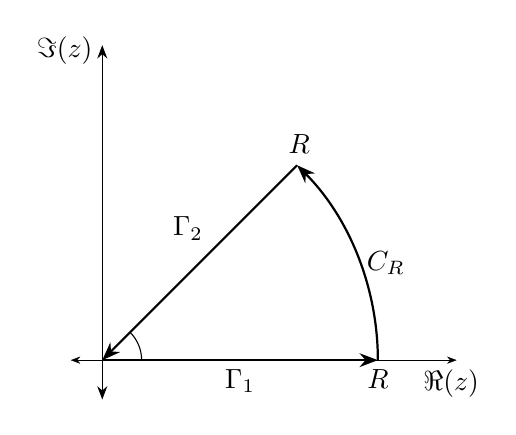
\begin{tikzpicture}[>=stealth,
                arrow style/.style={
                    postaction={decorate},
                    decoration={markings, mark=at position 0.5 with {\arrow[scale=1]{Stealth}}}
            }]

            \draw[-{Stealth}, ultra thin] (0, 0) -- (4.5, 0);
            \draw[-{Stealth}, ultra thin] (0, 0) -- (-0.4, 0);
            \draw[-{Stealth}, thin] (0, 0) -- (0, 4);
            \draw[-{Stealth}, thin] (0, 0) -- (0, -0.5);
            \draw[-{Stealth}, thick] (3.5,0) arc[start angle=0, end angle=45, radius=3.5];
            \draw[thin] (0.5,0) arc[start angle=0, end angle=45, radius=0.5];
            \draw[-{Stealth}, thick] (0, 0) -- (3.5, 0);
            \draw[-{Stealth}, thick] (2.47487, 2.47487) -- (0, 0);
            \node[anchor=north, xshift=-2pt] at (4.5, 0) {\(\Re(z)\)};
            \node[anchor=east, yshift=-2pt] at (0, 4) {\(\Im(z)\)};
            \node[anchor=north] at (1.75,0) {\(\Gamma_1\)};
            \node[anchor=south east] at (1.4,1.4) {\(\Gamma_2\)};
            \node[anchor=north] at (3.6,1.5) {\(C_R\)};
            \node[anchor=north] at (3.5,0) {\(R\)};
            \node[anchor=south] at (2.5,2.5) {\(R\)};
        \end{tikzpicture}
        \caption{A wedge contour with orientation marked.}\label{fig:wedgecontour}
    \end{figure}Let \(f(z)=\ee^{\ii z^2}\). Choose the wedge contour composed of
    \begin{gather*}
        \Gamma_1=\cbraces{x\in\mathbb{R}}{0\leq x\leq R},\qquad\Gamma_2=\cbraces{r\ee^{\ii\frac{\piup}{4}}}{0\leq r\leq R},\\
        C_R=\cbraces{R\ee^{\ii\theta}}{0\leq\theta\leq\frac{\piup}{4}}
    \end{gather*}
    as in \autoref{fig:wedgecontour}. By the Cauchy--Goursat Theorem (\autoref{thm:cauchygoursattheorem}), we have that
    \begin{equation}
        \int_{\Gamma_1}f(z)\ddz+\int_{\Gamma_2}f(z)\ddz+\int_{C_R}f(z)\ddz=0.\label{eq:fresnelwedgecontourintegral}
    \end{equation} The third integral can be written as \[\int_{C_R}f(z)\ddz=R\ii\int_0^{\frac{\piup}{4}}\exp[\ii{\qty(R\ee^{\ii\theta})}^2]\ee^{\ii\theta}\dd{\theta}.\]
    Using the fact that \(\frac{4}{\piup}\theta<\sin(2\theta)\) on the integration range, it can be bounded as
    \begin{align*}
        \abs{\int_{C_R}f(z)\ddz} & \leq R{\int_0^{\frac{\piup}{4}}\ee^{-R^2\sin(2\theta)}\dd{\theta}}<R\int_0^{\frac{\piup}{4}}\ee^{-\frac{4}{\piup}R^2\theta}\dd{\theta} \\
        & =-\frac{\piup}{4R}\eval{\ee^{-\frac{4}{\piup}R^2\theta}}_0^{\frac{\piup}{4}}=\frac{\piup}{4R}\qty(1-\ee^{-R^2}).
    \end{align*}
    As \(R\to\infty\), this integral tends to 0. Let \(z=r\ee^{\ii\frac{\piup}{4}}\) on \(\Gamma_2\). Then, we have \[\lim_{R\to\infty}\int_{\Gamma_2}f(z)\ddz=\int_\infty^0\exp[\ii\qty(r\ee^{\ii\frac{\piup}{4}})^2]\ee^{\ii\frac{\piup}{4}}\dd{r}=\ee^{\ii\frac{\piup}{4}}\int_\infty^0\exp(-r^2)\dd{r}.\]
    From equation~\eqref{eq:fresnelwedgecontourintegral}, we have that \[\int_0^\infty \ee^{\ii r^2}\dd{r}=\ee^{\ii\frac{\piup}{4}}\int_0^\infty \ee^{-r^2}\dd{r}.\] Since \(\int_0^\infty \ee^{-r^2}\dd{r}=\frac{\sqrt{\piup}}{2}\), we have \[\int_0^\infty \ee^{\ii r^2}\dd{r}=\qty(\frac{\sqrt{2}}{2}+\ii\frac{\sqrt{2}}{2})\frac{\sqrt{\piup}}{2}.\]
    Since \(\ee^{\ii r^2}=\cos(r^2)+\ii\sin(r^2)\), we have
    \begin{gather*}
        \int_0^\infty\cos(r^2)\dd{r}=\Re\qty[\int_0^\infty \ee^{\ii r^2}\dd{r}]=\frac{\sqrt{2\piup}}{4},\\
        \int_0^\infty\sin(r^2)\dd{r}=\Im\qty[\int_0^\infty \ee^{\ii r^2}\dd{r}]=\frac{\sqrt{2\piup}}{4},
    \end{gather*}
    as desired.
\end{proof}
\begin{example}
    Evaluate the integrals \(\int_0^{2\piup}\Phi(\cos\theta,\sin\theta)\dd{\theta}\), where \(\Phi(\xi,\eta)\) is a rational function of \(\xi\) and \(\eta\) that is continuous on \(\theta\in[0,2\piup]\).
\end{example}
\begin{proof}
    Let \(z=\ee^{\ii\theta}\). Consequently, we have \(\cos\theta=\frac{z+z^{-1}}{2}\), \(\sin\theta=\frac{z-z^{-1}}{2\ii}\), and \(\ddz=\ii\ee^{\ii\theta}\dd{\theta}\), implying that \(\dd{\theta}=\frac{\ddz}{\ii z}\). Therefore, by the Residue Theorem (\autoref{thm:residuethm}), letting \(f(z)=\frac{1}{\ii z}\Phi\qty(\frac{z+z^{-1}}{2},\frac{z-z^{-1}}{2\ii})\), we have \[\int_0^{2\piup}\Phi(\cos\theta,\sin\theta)\dd{\theta}=\int_{\partial\mathbb{D}}f(z)\ddz=2\piup\ii\sum_{k=1}^n\residue_{z=z_k}f(z),\]
    where \(z_k\) where \(k=1,\ldots,n\) are the isolated singularities of \(f\) in \(\mathbb{D}\).
\end{proof}
\begin{example}
    Evaluate \(I=\int_0^\infty\frac{x^\alpha}{1+x^\beta}\ddx\), where \(0<\alpha+1<\beta\).
\end{example}
\begin{proof}
    Let \(f(z)=\frac{z^\alpha}{1+z^\beta}\) and let \(-\piup<\Arg(z)\leq \piup\) in the principal branches of \(z^\alpha=\ee^{\alpha\Log(z)}\) and \(z^\beta=\ee^{\beta\Log(z)}\). Then except for at the zeros of \(1+z^\beta\), \(f\) is holomorphic.

    The solutions to \(z^\beta=-1\) are \(z=\exp(\ii\frac{\piup}{\beta}+2\ii k\frac{\piup}{\beta})\). Choose a wedge contour with an angle of \(\frac{2\piup}{\beta}\) (as in \autoref{fig:wedgecontour}). The only singularity it encloses is \(\exp(\ii\frac{\piup}{\beta})\). Since it is a simple zero of \(\frac{1}{f}\), this singularity is a simple pole.

    The contour is the union of the following curves:\
    \begin{gather*}
        \Gamma_1=\cbraces{x\in\mathbb{R}}{0\leq x\leq R},\qquad\Gamma_2=\cbraces{r\exp(\ii\frac{2\piup}{\beta})}{0\leq r\leq R},\\
        C_R=\cbraces{R\ee^{\ii\theta}}{0\leq\theta\leq \frac{2\piup}{\beta}},
    \end{gather*}
    where \(R>1\). By the Residue Theorem (\autoref{thm:residuethm}), we get that \[\lim_{R\to\infty}\int_{\Gamma_1}f(z)\ddz+\int_{\Gamma_2}f(z)\ddz+\int_{C_R}f(z)\ddz=2\piup\ii\Res[f,\exp(\ii\frac{\piup}{\beta})].\]
    By equation~\eqref{eq:residueatpole}, it follows that
    \begin{align*}
        \residue\qty[f,\exp(\ii\frac{\piup}{\beta})] & =\lim_{z\to\exp(\ii\frac{\piup}{\beta})}\flatfrac{\qty[z-\exp(\ii\frac{\piup}{\beta})]}{\qty[\frac{1+z^\beta}{z^\alpha}]} \\
        & =\lim_{z\to\exp(\ii\frac{\piup}{\beta})}{\dv{z}(z^{-\alpha}+z^{\beta-\alpha})}^{-1}                                     \\
        & =\lim_{z\to\exp(\ii\frac{\piup}{\beta})}\frac{z^{\alpha+1}}{(\beta-\alpha)z^{\beta}-\alpha}                             \\
        & =-\frac{1}{\beta}\exp(\ii\frac{\piup}{\beta}(\alpha+1)).
    \end{align*}
    We can write the integral on \(\Gamma_2\) in terms of \(I\):
    \begin{align*}
        \int_{\Gamma_2}f(z)\ddz & =\int_R^0 f\qty[r\exp(\ii\frac{2\piup}{\beta})]\exp(\ii\frac{2\piup}{\beta})\dd{r}   \\
        & =-\exp[\ii\frac{2\piup}{\beta}(1+\alpha)]\int_0^R\frac{r^\alpha}{1+r^\beta}\dd{r}.
    \end{align*}
    We also have \[\int_{C_R}f(z)\ddz=R\ii\int_{0}^{\frac{2\piup}{\beta}}f\qty(R\ee^{\ii\theta})\ee^{\ii\theta}\dd{\theta}=\ii\int_0^{\frac{2\piup}{\beta}}\frac{R^{\alpha+1}}{1+R^\beta \ee^{\ii\beta\theta}}\exp[\ii\theta(1+\alpha)]\dd{\theta}.\] We can show that the integrand can be dominated as follows:
    \[\abs{\int_0^{\frac{2\piup}{\beta}}\frac{R^{\alpha+1}}{1+R^\beta \ee^{\ii\beta\theta}}\exp[\ii\theta(1+\alpha)]\dd{\theta}}\leq\int_0^{\frac{2\piup}{\beta}}\frac{R^{\alpha+1}}{R^\beta-1}\dd{\theta}.\]
    The dominating integrand \(R\mapsto\frac{R^{\alpha+1}}{R^\beta-1}\) approaches \(0\) as \(R\to\infty\) since \(0<\alpha+1<\beta\). Therefore, \(\forall\varepsilon>0\), \(\exists N>2\) such that \(\forall R>N\), \(\frac{R^{\alpha+1}}{R^\beta-1}<\varepsilon\). Let \(\varepsilon\) be arbitrary. Then letting \(R>N\), the integrand is uniformly bounded, and therefore, \[\lim_{R\to\infty}\int_0^{\frac{2\piup}{\beta}}\frac{R^{\alpha+1}}{R^\beta-1}\dd{\theta}=\int_0^{\frac{2\piup}{\beta}}\lim_{R\to\infty}\frac{R^{\alpha+1}}{R^\beta-1}\dd{\theta}=0.\]
    By letting \(R\to\infty\), we have \[\qty[1-\exp(\ii\frac{2\piup}{\beta}(1+\alpha))]I=-\frac{2\piup\ii}{\beta}\exp(\ii\frac{\piup}{\beta}(\alpha+1)).\]
    It follows that \[I=\frac{2\piup\ii}{\beta}\brackets{\exp(\ii\frac{\piup}{\beta}(\alpha+1))-\exp(-\ii\frac{\piup}{\beta}(\alpha+1))}^{-1}=\frac{\piup}{\beta}\csc(\frac{\piup}{\beta}(\alpha+1)).\]
\end{proof}
\begin{example}
    Prove that the Fourier transform of \(\sech(\piup x)\) is itself, or that \[I(\xi)=\int_{-\infty}^\infty\exp(-2\piup \ii x\xi)\sech(\piup x)\ddx=\sech(\piup\xi).\]
\end{example}
\begin{proof}
    Fix \(\xi\in\mathbb{R}\) and let \(f(z)=\frac{\exp(-2\piup \ii z\xi)}{\cosh(\piup z)}\). Its poles in \(\mathbb{C}\) occur when \(\ee^{\piup z}+\ee^{-\piup z}=0\), or equivalently, when \(z=\ii\qty(n+\frac{1}{2})\), where \(n\in\mathbb{Z}\).

    \begin{figure}
        \centering
        \begin{tikzpicture}[>=stealth,
                arrow style/.style={
                    postaction={decorate},
                    decoration={markings, mark=at position 0.5 with {\arrow[scale=1]{Stealth}}}
            }]

            \draw[-{Stealth}, ultra thin] (0, 0) -- (5, 0);
            \draw[-{Stealth}, ultra thin] (0, 0) -- (-5, 0);
            \draw[-{Stealth}, thin] (0, 0) -- (0, 3);
            \draw[-{Stealth}, thin] (0, 0) -- (0, -0.5);
            \draw[-{Stealth}, thick] (-3, 0) -- (0, 0);
            \draw[-{Stealth}, thick] (0, 0) -- (3, 0);
            \draw[-{Stealth}, thick] (3, 0) -- (3, 2);
            \draw[-{Stealth}, thick] (3, 2) -- (0, 2);
            \draw[-{Stealth}, thick] (0, 2) -- (-3, 2);
            \draw[-{Stealth}, thick] (-3, 2) -- (-3, 0);
            \node[anchor=north, xshift=-2pt] at (5, 0) {\(\Re(z)\)};
            \node[anchor=east, yshift=-2pt] at (0, 3) {\(\Im(z)\)};
            \node[anchor=north] at (3,0) {\(R\)};
            \node[anchor=north] at (-3,0) {\(-R\)};
            \node[anchor=south east] at (0,2) {\(\ii\)};
        \end{tikzpicture}
        \caption{A rectangular contour with orientation marked.}\label{fig:rectangularcontour}
    \end{figure}Since \[\cosh(\piup(z+\ii))=-\cosh(\piup z),\qquad\exp(-2\piup\ii(z+\ii)\xi)=\exp(2\piup\xi)\exp(-2\piup \ii z\xi),\] we have that \(f(z)\) is a constant multiple of \(f(z+\ii)\). In particular, \(f(z+\ii)=-\exp(2\piup\xi)f(z)\). Therefore, we can use a rectangular contour as shown in \autoref{fig:rectangularcontour}. Let the sides be denoted by
    \begin{gather*}
        \overleftarrow{\Gamma}=\cbraces{x+\ii}{-R\leq x\leq R,x\in\mathbb{R}},\qquad\overrightarrow{\Gamma}x=\cbraces{x\in\mathbb{R}}{-R\leq x\leq R}\\
        \overset{\downarrow}{\Gamma}=\cbraces{-R+\ii y}{y\in[0,1]},\qquad\overset{\uparrow}{\Gamma}=\cbraces{R+\ii y}{y\in[0,1]}.
    \end{gather*}
    The only enclosed singularity is a simple pole at \(z=\frac{\ii}{2}\) (simple by evaluation of the Taylor expansion of the denominator). By the Residue Theorem (\autoref{thm:residuethm}), we get that
    \begin{equation}
        \qty(\int_{\overrightarrow{\Gamma}}+\int_{\overset{\uparrow}{\Gamma}}+\int_{\overleftarrow{\Gamma}}+\int_{\overset{\downarrow}{\Gamma}})f(z)\ddz=2\piup\ii\Res(f,\frac{\ii}{2}).\label{eq:fouriertransformofsechpix_rectangularcontourintegral}
    \end{equation}
    By equation~\eqref{eq:residueatpole}, we have
    \begin{align*}
        \Res(f,\frac{\ii}{2}) & =\lim_{z\to\frac{\ii}{2}}\qty(z-\frac{\ii}{2})\frac{\exp(-2\piup \ii z\xi)}{\cosh(\piup z)}      \\
        & =\lim_{z\to\frac{\ii}{2}}\dv{z}(\frac{\cosh(\piup z)}{\exp(-2\piup \ii z\xi)})^{-1}              \\
        & =\lim_{z\to\frac{\ii}{2}}\frac{\exp(-2\piup \ii z\xi)}{\piup\sinh(\piup z)+2\piup\ii\xi\cosh(\piup z)} \\
        & =\frac{\exp(\piup\xi)}{\piup \ii}.
    \end{align*}
    The sum of the horizontal line integrals is equal to
    \begin{align*}
        \int_{-R}^R f(z)\ddz+\int_R^{-R}f(z+\ii)\ddz & =\int_{-R}^R f(z)\ddz-\int_R^{-R}\ee^{2\piup\xi}f(z)\ddz \\
        & =\qty(1+\ee^{2\piup\xi})\int_{-R}^R f(z)\ddz.
    \end{align*} As \(R\to\infty\), we have \(\int_{\overrightarrow{\Gamma}}f(z)\ddz+\int_{\overleftarrow{\Gamma}}f(z)\ddz\to\qty(1+\ee^{2\piup\xi})I(\xi)\).
    The remaining two integrals can be written as
    \begin{align*}
        \int_{\overset{\uparrow}{\Gamma}}f(z)\ddz=\int_0^1 \frac{\exp(-2\piup\ii(R+\ii z)\xi)}{\cosh(\piup(R+\ii z))}\ddz \\
        \int_{\overset{\downarrow}{\Gamma}}f(z)\ddz=\int_1^0 \frac{\exp(2\piup\ii(R-\ii z)\xi)}{\cosh(\piup(-R+\ii z))}\ddz.
    \end{align*}
    They can be bounded with
    \begin{align*}
        \abs{\int_0^1 \frac{\exp(-2\piup\ii(R+\ii z)\xi)}{\cosh(\piup(R+\ii z))}\ddz} & \leq 2\int_0^1\frac{\exp(2\piup z\xi)}{\abs{\ee^{\piup R}\ee^{\piup \ii z}+\ee^{-\piup R}\ee^{-\piup \ii z}}}\ddz \\
        & \leq2\int_0^1\frac{\exp(2\piup z\xi)}{\abs{\ee^{\piup R}-\ee^{-\piup R}}}\ddz
    \end{align*} and
    \begin{align*}
        \abs{\int_1^0 \frac{\exp(2\piup\ii(R-\ii z)\xi)}{\cosh(\piup(-R+\ii z))}\ddz} & \leq 2\int_0^1\frac{\exp(2\piup z\xi)}{\abs{\ee^{-\piup R}\ee^{\piup \ii z}+\ee^{\piup R}\ee^{-\piup \ii z}}}\ddz \\
        & \leq2\int_0^1\frac{\exp(2\piup z\xi)}{\abs{\ee^{\piup R}-\ee^{-\piup R}}}\ddz
    \end{align*}
    Since the integrands are continuous and uniformly convergent to \(0\) with respect to \(z\), we have \[\int_{\overset{\uparrow}{\Gamma}}f(z)\ddz+\int_{\overset{\downarrow}{\Gamma}}f(z)\ddz\to 0\] as \(R\to\infty\). By rearrangement of equation~\eqref{eq:fouriertransformofsechpix_rectangularcontourintegral}, \[I(\xi)\qty(1+\ee^{2\piup\xi})=2\exp(\piup\xi),\]
    or that \[I(\xi)=\frac{2}{\ee^{-\piup\xi}+\ee^{\piup\xi}}=\sech(\piup\xi),\] which proves the result.
\end{proof}
Contour integration provides a powerful method for evaluating real improper integrals by leveraging the Residue Theorem (\autoref{thm:residuethm}). The primary challenge often lies in constructing a suitable contour in the complex plane that encloses the relevant singularities of the integrand \(f\) while ensuring that the contribution from the contributions from the remaining segments of the contour either vanishes or can be calculated with ease.

If the function \(f\) is even and integrated on a domain such as \(\mathbb{R}_{\geq0}\), then the integral can be extended to the entire real axis. If \(f\) decays sufficiently rapidly in the upper half plane \(\mathbb{H}^+\), a semicircular contour is generally preferable, as illustrated in \autoref{fig:semicircularcontour}. In the presence of singularities on the contour itself, we can insert arc indentations around them, as shown in \autoref{fig:indentedsemicircularcontour}.

If \(f(z)\) is a constant multiple of \(f(z+\ii y)\) for some \(y\in\mathbb{R}\), it is a strong indication to use a rectangular contour. If \(f(z)\) is a constant multiple of \(f\qty(z\ee^{\ii\tau})\) for some \(\tau\in\mathbb{R}\), a wedge-shaped contour is an appropriate choice.

The following result is useful for evaluating integrals on indentations along a contour.
\begin{theorem}\label{thm:residueoverarc}
    Let \(\lambda>0\) and let \(a\in\mathbb{C}\). Suppose \(f(z)\) is a holomorphic function on \(D^*(a,\lambda)\) with a simple pole at \(z=a\in U\). Let \(0<\varepsilon<\lambda\) and define \(\gamma_\varepsilon\subseteq\partial D(a, \varepsilon)\) be a counterclockwise-oriented, connected arc subtending an angle \(\vartheta\). Then,
    \[\lim_{\varepsilon\to 0}\int_{\gamma_\varepsilon}f(z)\ddz=\ii\vartheta\cdot\residue_{z=a}f(z).\]
\end{theorem}
\begin{proof}
    Parameterize \(\gamma_\varepsilon\) with \(z=a+\varepsilon \ee^{\ii\theta}\), where \(\theta\in[\alpha,\beta]\) and \(\beta-\alpha=\vartheta\). Then,
    \[\int_{\gamma_\varepsilon} f(z)\ddz = \int_\alpha^\beta f\qty(a+\varepsilon \ee^{\ii\theta}) \dv{z}{\theta}\dd{\theta}=\varepsilon \ii \int_\alpha^\beta f\qty(a+\varepsilon \ee^{\ii\theta})\ee^{\ii\theta}\dd{\theta}.\]
    Since \(f\) has a simple pole at \(z=a\), we can write a Laurent expansion around \(a\) as
    \[f(z)=\frac{c_{-1}}{z-a}+\varphi(z),\]
    where \(\varphi(z)\) is holomorphic in a neighborhood of \(a\) and \(c_{-1}=\residue_{z=a}f(z)\).

    Then for \(z=a+\varepsilon \ee^{\ii\theta}\),
    \[f\qty(a+\varepsilon \ee^{\ii\theta})=\frac{c_{-1}}{\varepsilon \ee^{\ii\theta}}+\varphi\qty(a+\varepsilon \ee^{\ii\theta}).\]
    So,
    \begin{align*}
        \int_{\gamma_\varepsilon}f(z)\ddz
        & = \varepsilon \ii\int_\alpha^\beta \qty(\frac{c_{-1}}{\varepsilon\ee^{\ii\theta}}+\varphi\qty(a+\varepsilon\ee^{\ii\theta}))\ee^{\ii\theta}\dd{\theta} \\
        & = \ii c_{-1}\int_\alpha^\beta\dd{\theta}+\varepsilon \ii\int_\alpha^\beta\varphi\qty(a+\varepsilon \ee^{\ii\theta})\ee^{\ii\theta}\dd{\theta}          \\
        & = \ii c_{-1}\vartheta+\varepsilon \ii\int_\alpha^\beta\varphi\qty(a+\varepsilon\ee^{\ii\theta})\ee^{\ii\theta}\dd{\theta}.
    \end{align*}
    Let \(\varepsilon<\frac{\lambda}{2}\). Since \(\varphi\) is continuous on the disk \(\overline{D\qty(a,\frac{\lambda}{2})}\), it is bounded. Therefore, letting \(\varepsilon\to0\), we have
    \[\lim_{\varepsilon\to 0} \varepsilon \ii \int_\alpha^\beta\varphi\qty(a+\varepsilon\ee^{\ii\theta})\ee^{\ii\theta}\dd{\theta}=\lim_{\varepsilon\to 0}\varepsilon \ii\int_\alpha^\beta\varphi(a)\ee^{\ii\theta}\dd{\theta}=0.\]
    Therefore,
    \[\lim_{\varepsilon \to 0}\int_{\gamma_\varepsilon}f(z)\ddz=\ii\vartheta\residue_{z=a}f(z),\] as desired.
\end{proof}
\section{Analytic Continuation}\label{sec:analyticcontinuation}
\subsection{Analytic Function Elements}
\begin{definition}\label{def:analyticelement}
    An \textit{analytic function element} is a pair \((f,U)\), where \(U\subseteq\mathbb{C}\) is an open disk and \(f\) is a holomorphic function on \(U\).
\end{definition}
Analytic elements serve as local representations of analytic functions. The process of extending these elements is formalized through \textit{analytic continuation}, previously introduced in \autoref{def:analyticcontinuation}.

By the Identity Theorem (\autoref{thm:identity}), such continuations are unique; if \(\qty(f_1,U_1)\) and \(\qty(f_2,U_2)\) are analytic elements with \(U_1\cap U_2 \neq \emptyset\), and \(f_1\equiv f_2\) on \(U_1\cap U_2\), then they are \textit{direct analytic continuations} of each other. The combined function:
\[\widetilde{f}(z)=
    \begin{cases}
        f_1(z) & z\in U_1               \\
        f_2(z) & z\in U_2 \setminus U_1
\end{cases}\] is holomorphic on \(U_1\cup U_2\).

The most straightforward method of the derivation of analytic continuations uses power series. Let \(f(z)=\sum_{n=0}^{\infty}c_n\qty(z-z_0)^n\) have radius of convergence \(R>0\) (by \autoref{thm:abelradius}). For \(z_1\in D\qty(z_0,R)\), we can expand \(f\) at \(z_1\):
\[f(z)=\sum_{k=0}^\infty\frac{f^{(k)}\qty(z_1)}{k!}\qty(z-z_1)^k.\]
Let \(\rho\) be the radius of convergence of this series. Then:
\[\rho\geq R-\abs{z_1-z_0}.\]
If \(\rho>R-\abs{z_1-z_0}\), then \(f\) extends analytically to \(D\qty(z_0,R) \cup D(z_1,\rho)\). In the case that \(\rho=R-\abs{z_1-z_0}\), the disks \(D\qty(z_0,R)\) and \(D\qty(z_1,\rho)\) are tangent at a point \(\zeta_0\). Here, \(\zeta_0\) is a \textit{singularity}, and \(f\) cannot be continued beyond \(\zeta_0\).
\begin{theorem}\label{thm:boundarysingularity}
    Let \(f(z)=\sum_{n=0}^{\infty}c_n{\qty(z-z_0)}^n\) have radius of convergence \(R>0\). Then \(\partial D\qty(z_0,R)\) contains at least one singularity of \(f\).
\end{theorem}
\begin{proof}
    Assume \(f\) can be analytically continued from every \(\zeta\in\partial D\qty(z_0,R)\). Then for each \(\zeta\), there exists \(r_\zeta>0\) and a holomorphic \(f_\zeta\) on \(D\qty(\zeta,r_\zeta)\) agreeing with \(f\) on \(D\qty(\zeta,r_\zeta) \cap D\qty(z_0,R)\).

    The disks \(\cbraces{D\qty(\zeta,r_\zeta)}_{\zeta \in\partial D\qty(z_0,R)}\) cover the compact set \(\partial D\qty(z_0,R)\). By the Heine--Borel Theorem (\autoref{thm:heineborel}), they admit a finite subcover \(\qty{D\qty(\zeta_k,r_k)}_{k=1}^n\). Thus, \(\exists\rho>0\) such that \(A=\cbraces{z}{R-\rho\leq\abs{z-z_0}\leq R+\rho}\subset V\), where \(V=\bigcup_{k=1}^n D\qty(\zeta_k,r_k)\).

    Define \(\Phi:V\to\mathbb{C}\) by \(\Phi(z)=f_{\zeta_k}(z)\) if \(z\in D\qty(\zeta_k,r_k)\). This is well-defined: If \(z\in D\qty(\zeta_i,r_i)\cap D\qty(\zeta_j,r_j)\), then \(D\qty(\zeta_i,r_i)\cap D\qty(\zeta_j,r_j) \cap D\qty(z_0,R)\neq\emptyset\), and \(f_{\zeta_i}=f_{\zeta_j}=f\) there. By the Identity Theorem (\autoref{thm:identity}), \(f_{\zeta_i}\equiv f_{\zeta_j}\) on \(D\qty(\zeta_i,r_i)\cap D\qty(\zeta_j,r_j)\).

    Since \(\Phi\) is holomorphic on \(V\) and agrees with \(f\) on \(D\qty(z_0,R)\cap V\), the function:
    \[\widetilde{f}(z)=
        \begin{cases}
            f(z)    & z\in D\qty(z_0,R) \\
            \Phi(z) & z\in V
    \end{cases}\]
    is holomorphic on \(D\qty(z_0,R)\cup V\supset D(z_0, R+\rho)\), contradicting the maximality of \(R\).
\end{proof}
\begin{definition}[Maximal Analytic Continuation]\label{def:maximalanalyticcontinuation}
    A \textit{maximal analytic continuation} \(\qty(\widetilde{f},\widetilde{U})\) is an analytic element that has no analytic continuation to a larger domain. The set \(\widetilde{U}\) is known as the \textit{domain of holomorphy} of \(\widetilde{f}\). The boundary set \(\partial\widetilde{U}\) is known as a \textit{natural boundary}. Here, \(\widetilde{f}\) is known as a \textit{complete analytic function}, which can be multi-valued.
\end{definition}
\begin{example}\label{ex:factoriallacunaryseries}
    The series \(f(z)=\sum_{n=0}^{\infty}z^{n!}\) has \(\mathbb{D}\) as its disk of convergence, and every point on \(\partial\mathbb{D}\) is a singularity.
\end{example}
\begin{proof}
    By Cauchy--Hadamard (\autoref{thm:cauchyhadamard}), \(\varlimsup_{n\to\infty}\sqrt[n]{\abs{c_n}}=1\) since \(c_n=1\) if \(n=k!\) and \(0\) otherwise. Thus, \(R=1\).

    Fix \(\zeta\in\partial\mathbb{D}\). Suppose \(f\) extends analytically to a disk \(D(\zeta,\delta)\). Since \(\exp(2\piup\ii\mathbb{Q})\) is dense in \(\partial\mathbb{D}\), there exists \(\zeta'=\exp(2\piup\ii\frac{p}{q})\in D(\zeta,\delta)\cap\partial\mathbb{D}\) for coprime integers \(p,q\). The extension \(g\) of \(f\) to \(D(\zeta, \delta)\) would satisfy:
    \[\lim_{r\to1^{-}}f(r\zeta')=g(\zeta').\]
    However, for \(0<r<1\):
    \[f(r\zeta')=\sum_{k=0}^{q-1}{\qty(r\zeta')}^{k!}+\sum_{k=q}^\infty r^{k!}\zeta'^{k!}.\]
    The second summation is unbounded since \[\sum_{k=q}^\infty r^{k!}\zeta'^{k!}=\sum_{k=q}^\infty r^{k!}>\sum_{k=q}^N r^{k!}>(N-q+1)r^{N!}\] for any integer with \(N>q\). Hence, as \(r\to1^-\), \(\sum_{k=q}^{\infty} r^{k!}\to\infty\). Hence, \(\zeta\) is a singularity.
\end{proof}
\begin{example}
    Show that \(f(z)=\sum_{n=0}^\infty z^{2^n}\) cannot be analytically continued to the outside of \(\mathbb{D}\).
\end{example}
\begin{proof}
    Trivially, at \(z=1\), the series diverges. Therefore, \(\mathbb{D}\) is its convergence disk. Observe that \(f(z)=\sum_{n=0}^\infty \qty(z^2)^{2^{n-1}}=\sum_{n=0}^\infty \qty(z^2)^{2^n}+z=f\qty(z^2)+z\). Hence, we have \[f(z)=f\qty(z^2)+z=f\qty(z^4)+z^2+z=f\qty(z^8)+z^4+z^2+z\cdots,\]
    which diverges at each \(z^2,z^4,z^8,\ldots=1\). The solutions form a dense set in \(\partial\mathbb{D}\). By the same reasoning as \autoref{ex:factoriallacunaryseries}, \(f\) cannot be analytically continued to the outside of \(\mathbb{D}\).
\end{proof}
\begin{example}\label{ex:complexlogarithmanalyticcontinuation}
    Let \(\Log(z)\) denote the principal branch of \(\log(z)\), with \(-\piup<\Arg(z)\leq\piup\). The analytic function elements \[\qty(\Log,D(1,1))\qand\qty(\Log+2\piup\ii,D(1,1))\] are analytic continuations of each other.
\end{example}
\begin{example}
    Show that the analytic functions defined by the series \(f(z)=\sum_{n=0}^\infty\alpha^n z^n\) and \(\widetilde{f}(z)=\sum_{n=0}^\infty\frac{(\alpha-1)^n z^n}{{\qty(1-z)}^{n+1}}\) are analytic continuations of each other.
\end{example}
\begin{proof}
    The analytic function element \(\qty(f,D\qty(0,\abs{\frac{1}{\alpha}}))\) can be directly continued to the analytic function element \(\qty(z\mapsto\frac{1}{1-\alpha z},\mathbb{C}\setminus\qty{\frac{1}{\alpha}})\). The function element \(\qty(\widetilde{f},D\qty(0,\frac{1-z}{\alpha-1}))\) can be analytically continued to \[\qty(z\mapsto\frac{1}{(1-z)\qty(1-\frac{z\alpha-z}{1-z})},\mathbb{C}\setminus\qty{1,\frac{1}{\alpha}})=\qty(z\mapsto\frac{1}{1-\alpha z},\mathbb{C}\setminus\qty{1,\frac{1}{\alpha}}),\] which is a direction analytic continuation of \(\qty(z\mapsto\frac{1}{1-\alpha z},\mathbb{C}\setminus\qty{\frac{1}{\alpha}})\). Therefore, \(f\) and \(\widetilde{f}\) are analytic continuations of each other.
\end{proof}
In \autoref{ex:complexlogarithmanalyticcontinuation}, we showed that two analytic function elements can on the same domain can be analytic continuations even if they do not agree on all of the domain. In this case, the two elements are branches of the function. In other words, depending on the chain of function elements chosen, we may obtain two different analytic function elements that have the same domain.

This is a common issue when it comes to the problem of analytic continuation. This question of non-ambiguity can be explained by planar topology; specifically the concept of homotopy. We will now introduce the concept of analytic continuation along a given curve.
\subsection{Analytic Continuation Along a Curve}
\begin{definition}\label{def:analyticcontinuationalongcurve}
    Let \(\gamma:[0,1]\to\mathbb{C}\) be a (non-constant) curve. Let \(U\) be a disk centered at \(\gamma(0)\) and suppose \(f: U\to\mathbb{C}\) is holomorphic. An \textit{analytic continuation of} \(\qty(f,U)\) \textit{along} \(\gamma\) is an uncountable collection of analytic function elements \(\cbraces{\qty(f_t, U_t)}{0\leq t\leq 1}\) where
    \begin{enumerate}
        \item We define \(U_0=U\) and \(f_0=f\).
        \item Each \(U_t\) (\(0\leq t\leq 1\)) is a disk centered at \(\gamma(t)\).
        \item For each \(t_0\in [0,1]\), \(\exists\delta>0\) such that \(\forall t\in[0,1]\) satisfying \(\abs{t-t_0}<\delta\), \(\gamma(t)\in U_{t_0}\) and \(f_t\equiv f_{t_0}\) on \(U_t\cap U_{t_0}\neq\emptyset\).\label{itm:analyticcontinuationalongcurve_pointwiseequivalence}
    \end{enumerate}
\end{definition}
For a fixed curve, such analytic continuations are unique in the following sense:
\begin{lemma}
    For a fixed curve \(\gamma:[0,1]\to\mathbb{C}\), let \(f\) be holomorphic on \(U\) (a disk centered at \(\gamma(0)\)). Then any two analytic continuations along \(\gamma\), namely \(\qty{\qty(f_t,U_t)}_{0\leq t\leq 1}\) and \(\qty{\qty(\widetilde{f}_t,\widetilde{U}_t)}_{0\leq t\leq 1}\) satisfy \(f_1\equiv\widetilde{f}_1\) on \(U_1\cap\widetilde{U}_1\) (where \(\qty(f_1,U_1)\) and \(\qty(\widetilde{f}_t,\widetilde{U}_t)\) are the respective terminal analytic function elements).
\end{lemma}
\begin{proof}
    Let \(S\subseteq[0,1]\) be the set of all \(t_0\) such that \(\forall 0\leq t\leq t_0\), \(f_t\equiv \widetilde{f}_t\) on \(U_t\cap\widetilde{U}_t\) (this intersection is nonempty since \(\gamma(t)\in U_t,\widetilde{U}_t\)). Since \(0\in S\), it follows that \(S\) is nonempty.

    Obviously, \(S\) is a connected set. Indeed, for any \(t_0\) in \(S\), any \(0\leq t<t_0\) also lies in \(S\) by definition.

    Let \(t_\infty=\sup(S)\), and choose an increasing sequence \(\qty{t_n}_{n\in\mathbb{N}}\subseteq S\) that converges to \(t_\infty\). By~\ref{itm:analyticcontinuationalongcurve_pointwiseequivalence} of \autoref{def:analyticcontinuationalongcurve}, \(\exists\delta>0\) such that \(\forall n\in\mathbb{N}\) satisfying \(\abs{t_\infty-t_n}<\delta\), \[f_{t_n}\equiv f_{t_\infty}\qq{on} U_{t_n}\cap U_{t_\infty}.\] Similarly, \(\exists\widetilde{\delta}>0\) such that \(\forall n\in\mathbb{N}\) satisfying \(\abs{t_\infty-t_n}<\widetilde{\delta}\), \[\widetilde{f}_{t_n}\equiv\widetilde{f}_{t_\infty}\qq{on}\widetilde{U}_{t_n}\cap\widetilde{U}_{t_\infty}.\]
    Choose \(n\) arbitrarily to satisfy \(\abs{t_\infty-t_n}<\min\qty(\delta,\widetilde{\delta})\). By definition, \[\gamma\qty(t_n)\in U_{t_\infty}\qand \gamma\qty(t_n)\in\widetilde{U}_{t_\infty}.\] Hence, \(\widetilde{U}_{t_\infty}\cap U_{t_\infty}\cap \widetilde{U}_{t_n}\cap U_{t_n}\neq\emptyset\). Since \(t_n\in S\), it follows that \(\widetilde{f}_{t_n}\equiv f_{t_n}\) on \(\widetilde{U}_{t_n}\cap U_{t_n}\). Thus, \[f_{t_\infty}\equiv\widetilde{f}_{t_\infty}\qq{on}\widetilde{U}_{t_\infty}\cap U_{t_\infty}\cap \widetilde{U}_{t_n}\cap U_{t_n}.\] By the Identity Theorem (\autoref{thm:identity}), this equality holds on the entire intersection \(\widetilde{U}_{t_\infty}\cap U_{t_\infty}\). It follows that \(t_\infty\in S\) and thus \(S\) is closed.

    Let \(\widetilde{S}=[0,1]\setminus S\). Let \(\qty{t_n}\subset\widetilde{S}\) be an arbitrary sequence that converges to \(t_\infty\).
\end{proof}
\subsection{The Monodromy Theorem}
\section{Rational Approximation Theory}
\section{The Theory of Riemann}\label{sec:riemann}
\subsection{Biholomorphy}
In \chpref{sec:conformalityintroduction}, it was asserted that for a holomorphic function \(f(z)\), the map \(w=f(z)\) is conformal when \(f'(z)\neq 0\).

We have the following immediate assertion:
\begin{theorem}[Open Mapping Theorem]\label{thm:openmapping}
    Let \(U\subseteq\mathbb{C}\) be a region (open, nonempty, and connected). Let \(f:U\to\mathbb{C}\) be holomorphic and non-constant. Then the image \(f(U)\) is a region.
\end{theorem}
\begin{proof}
    The nonemptiness of \(f(U)\) is an immediate conclusion from the fact that \(U\) is nonempty and \(f\) is defined on all of \(U\).

    Let \(w_0\) be an arbitrary point in \(f(U)\). Then \(\exists z_0\in U\) such that \(f\qty(z_0)=w_0\). Since \(f\) is non-constant, the function \(f-w_0\) has an isolated zero at \(z_0\). Thus for sufficiently small \(\rho>0\), the only zero of \(f-w_0\) in \(\overline{D\qty(z_0,\rho)}\) is at \(z_0\).

    By \autoref{thm:hurwitzshifts}, then there exists \(\delta>0\) such that \(\forall\varepsilon\in D(0,\delta)\), \(f(z)-w_0-\varepsilon\) has exactly one zero in \(\overline{D\qty(z_0,\rho)}\). In other words, \(\forall w_0\in f(U)\), \(\exists\delta>0\) such that \(\forall w\in D\qty(w_0,\delta)\), \(\exists! z\in\overline{D\qty(z_0,\rho)}\) such that \(f(z)=w\). Thus, \(f\qty(D\qty(w_0,\delta))\subseteq f(U)\). Thus, \(f(U)\) is an open set since each contained point has a fully contained open neighborhood.

    Let \(w_1,w_2\in f(U)\) be arbitrary and distinct. Then there exist \(z_1, z_2\in U\) such that \(f\qty(z_1)=w_1\) and \(f\qty(z_2)=w_2\). By the connectivity of \(U\), there exists a path \(\gamma\subset U\) that connects \(z_1\) and \(z_2\). Then \(f(\gamma)\subset f(U)\) is a curve that joins \(w_1\) and \(w_2\). Thus, \(f(U)\) is connected.
\end{proof}
Holomorphic injectivity, or univalence, satisfies the proceeding assertion:
\begin{lemma}\label{lemma:univalentnonvanishingderivative}
    Let \(U\subseteq\mathbb{C}\) be a region and suppose \(f:U\to\mathbb{C}\) is univalent. Then \(f'\) is non-vanishing on \(U\).
\end{lemma}
\begin{proof}
    Suppose, for the sake of contradiction, that \(f\) is univalent on \(U\) such that \(\exists z_0\in U\) such that \(f'\qty(z_0)=0\). Let \(w_0=f\qty(z_0)\). The previous statement is equivalent to: \(f(z)-w_0\) has a zero at \(z_0\) with multiplicity \(m\geq 2\).

    Since this zero is isolated, let \(\rho>0\) be chosen such that \(z_0\) is the only zero of \(f-w_0\) contained in \(\overline{D\qty(z_0,\rho)}\subset U\). By \autoref{thm:hurwitzshifts}, \(\exists \delta>0\) such that \(\forall w\in D\qty(w_0,\delta)\), the equation \(f(z)=w\) has \(m\) solutions in \(\overline{D\qty(z_0,\rho)}\). This contradicts the univalence of \(f\).
\end{proof}
Conversely, we have the following statement on local univalence and invertibility.
\begin{lemma}
    Let \(U\subseteq\mathbb{C}\) be a region and suppose \(f:U\to\mathbb{C}\) is holomorphic. If \(f'\qty(z_0)\neq0\) for some \(z_0\in U\), then there exists an open neighborhood of \(z_0\) on which \(f\) is univalent.
\end{lemma}
\begin{proof}
    Let \(w_0=f\qty(z_0)\). Since \(\lim_{z\to z_0}f(z)-w_0=0\) and \(\lim_{z\to z_0}\frac{f(z)-w_0}{z-z_0}\neq0\), it follows that \(z_0\) is a simple zero of \(f(z)-w_0\). Let \(V\) be an open neighborhood (relatively compact in \(U\)) of \(z_0\) whose closure does not contain other zeros of \(f-w_0\). By \autoref{thm:hurwitzshifts}, \(\exists\delta>0\) such that \(\forall w\in D\qty(w_0,\delta)\), \(f(z)=w\) has only one solution for \(z\) satisfying \(z\in V\). Therefore, we can choose a relatively compact open subset \(W\) of \(V\) such that \(f\qty(W)\subseteq D\qty(w_0,\delta)\), on which \(f\) is univalent.
\end{proof}
Moreover, if \(w=f(z)\) is univalent and surjective, mapping \(U\) to \(G\), then its inverse \(z=f^{-1}(w)\) is univalent on \(G\). Such bijective holomorphic functions are known as \textit{biholomorphisms} or \textit{biholomorphic} functions.

We will now study holomorphic functions from a more geometric perspective.
\begin{theorem}\label{thm:boundaryofconformalmap}
    Let \(\Omega\subseteq\mathbb{C}\) be a region, and let \(\gamma\subset\Omega\) be a rectifiable simple closed counterclockwise-oriented curve that is null-homotopic in \(\Omega\). Denote \(\mathrm{int}(\gamma)\) by \(U\). If \(f:\Omega\to\mathbb{C}\) is holomorphic and maps \(\gamma\) injectively to a simple closed curve \(\Gamma\), then \(w=f(z)\) is univalent in \(U\), \(f(U)=\mathrm{int}(\Gamma)\), and \(\Gamma\) is traversed counterclockwise.
\end{theorem}
\begin{proof}
    Let \(w_0\in\mathbb{C}\). First \(w_0\) does not lie on \(\Gamma\) itself. By the Argument Principle (\autoref{thm:argumentprincipleholomorphic}), the number of zeros of \(f-w_0\) enclosed by \(\gamma\) is equal to \[k=\frac{1}{2\piup \ii}\oint_\gamma \frac{f'(z)}{f(z)-w_0}\ddz=\frac{1}{2\piup \ii}\oint_\Gamma\frac{\dd{w}}{w-w_0}=\frac{1}{2\piup}\Delta_\Gamma\arg(w-w_0).\] If \(w_0\in\mathrm{ext}(\Gamma)\), the integral vanishes by the Cauchy--Goursat Theorem (\autoref{thm:cauchygoursattheorem}). On the contrary, if \(w_0\in\mathrm{int}(\Gamma)\), then \(\Gamma\) winds around \(w_0\) exactly once, and hence, in other words, \(\forall w_0\in\mathrm{int}(\Gamma)\), \(f(z)=w_0\) has a unique solution in \(U\). This verifies the univalence of \(f\) in \(U\).

    If \(w_0\) lies on \(\Gamma\), \(f-w_0\) has no zeros in \(U\). Indeed, for the sake of contradiction, assume that \(\exists z_0\in U\) such that \(f\qty(z_0)=w_0\). By the Open Mapping Theorem (\autoref{thm:openmapping}) and \autoref{thm:hurwitzshifts}, \(\exists\delta>0\) such that \(D\qty(w_0,\delta)\subseteq f(U)\) and \(\forall w'\in D\qty(w_0,\delta)\), \(f-w'\) has zeros in \(U\). Since \(w_0\) lies on \(\Gamma\), a subset of \(D\qty(w_0,\delta)\) lies in the exterior of \(\Gamma\). It was previously established that \(f-w'\) has no zeros if \(w'\in D\qty(w_0,\delta)\cap\mathrm{ext}(\Gamma)\). Thus, we have a contradiction. We then have \[k=
        \begin{cases}
            0 & w_0\in\overline{\mathrm{ext}(\Gamma)} \\
            1 & w_0\in \mathrm{int}(\Gamma)
    \end{cases}.\]
    Hence, for any arbitrary \(z_0\in U\), \(w_0=f\qty(z_0)\) must lie in \(\mathrm{int}(\Gamma)\). Indeed, if \(f\qty(z_0)\) lies in \(\mathrm{ext}(\Gamma)\) or \(\Gamma\), then \(k\) would be nonzero in those areas. It follows that \(f(U)=\mathrm{int}(\Gamma)\).
\end{proof}
We will now give examples of biholomorphisms.
\begin{example}
    The only biholomorphisms which map \(\mathbb{D}\) to itself are in the form of
    \begin{equation}
        w=\ee^{\ii\theta}\frac{z-a}{1-\overline{a}z},\quad a\in\mathbb{D},\theta\in\mathbb{R}.\label{eq:biholomorphismunitdiskautomorphism}
    \end{equation}
    This follows directly from \autoref{thm:holomorphicautomorphismgrouponunitdisk}.
\end{example}
\begin{example}\label{ex:biholomorphismsupperhalfplanetounitdisk}
    The only biholomorphisms which map \(\mathbb{H}^+\) to \(\mathbb{D}\) are in the form of
    \begin{equation}
        w=\ee^{\ii\theta}\frac{z-a}{z-\overline{a}},\quad a\in\mathbb{H}^+,\theta\in\mathbb{R}.\label{eq:biholomorphismunitdisktoupperhalfplane}
    \end{equation}
\end{example}
\begin{proof}
    First assume \(y=\Im(z)>0\). It follows that \[\abs{w}=\abs{\frac{z-a}{z-\overline{a}}}=\sqrt{\frac{\qty(x-\Re(a))^2+\qty(y-\Im(a))^2}{\qty(x-\Re(a))^2+\qty(y+\Im(a))^2}}<1.\] Therefore, this transformation maps \(\mathbb{H}^+\) to \(\mathbb{D}\). The inverse mapping is equal to
    \begin{equation}
        z=\frac{w\overline{a}-a\ee^{\ii\theta}}{w-\ee^{\ii\theta}}.\label{eq:biholomorphismunitdisktoupperhalfplane_inverse}
    \end{equation}
    Assume \(w\in\mathbb{D}\). We then have
    \begin{align*}
        \Im(z)=\Im\frac{\qty(w\overline{a}-a\ee^{\ii\theta})\qty(\overline{w}-\ee^{-\ii\theta})}{\abs{w-\ee^{\ii\theta}}^2}&=\frac{\abs{w}^2\Im\qty(\overline{a})-\Im\qty(a\ee^{\ii\theta}\overline{w})-\Im\qty(w\overline{a}\ee^{-\ii\theta})+\Im(a)}{\abs{w-\ee^{\ii\theta}}^2}\\
        &=\frac{\qty(1-\abs{w}^2)\Im\qty(a)}{\abs{w-\ee^{\ii\theta}}^2}>0.
    \end{align*}
    Hence, \(z\) maps \(\mathbb{D}\) to \(\mathbb{H}^+\) univalently and surjectively since it is also an element in \(\Aut\qty(\extcomplex)\).

    Let \(\psi(z)\) be the biholomorphism from \(\mathbb{H}^+\) to \(\mathbb{D}\) in the form of \(\psi(z)=\frac{z-\ii}{z+\ii}\) (for \(\theta=0\) and \(a=\ii\)). Let \(f\) be an arbitrary biholomorphism from \(\mathbb{H}^+\) to \(\mathbb{D}\). It follows that \(\varphi=f\circ\psi^{-1}\) is a holomorphic automorphism of \(\mathbb{D}\). Since \(\varphi\in\Aut(\mathbb{D})\), we have \[f(z)=\varphi\circ\psi(z)=\ee^{\ii\theta}\frac{z\qty(1-a)-\ii\qty(a+1)}{z\qty(1-\overline{a})+\ii\qty(\overline{a}+1)}=\ee^{\ii\theta}\frac{z\frac{1-a}{1-\overline{a}}+\ii\frac{a+1}{\overline{a}-1}}{z-\ii\frac{\overline{a}+1}{\overline{a}-1}}=\ee^{\ii\theta}\frac{1-a}{1-\overline{a}}\frac{z-\ii\frac{a+1}{1-a}}{z-\overline{\ii\frac{a+1}{1-a}}}.\]
    Obviously, \(\ee^{\ii\theta}\frac{1-a}{1-\overline{a}}\) attains every value on the unit disk for varying \(a\) and \(\theta\). Similarly, the values attained by \(\ii\frac{a+1}{1-a}\) cover the upper half-plane for \(a\in\mathbb{D}\) (since it is in the form of equation~\eqref{eq:biholomorphismunitdisktoupperhalfplane_inverse}). Thus, all biholomorphisms from \(\mathbb{H}^+\) to \(\mathbb{D}\) are in the form of equation~\eqref{eq:biholomorphismunitdisktoupperhalfplane}.
\end{proof}
Let us now introduce some important properties of linear fractional transformations. By \autoref{lemma:mobiustransformationcompositionmatrixmultiplication}, it follows that the composition of two linear fractional transformations is also a linear fractional transformation.
\begin{theorem}\label{thm:linearfractionaltransformationmapscirclestocircles}
    Let \(\mathcal{C}\) be the collection of subsets of \(\extcomplex\) that are circles or \(L\cup\qty{\infty}\), where \(L\) is a straight line in \(\mathbb{C}\). Then every linear fractional transformation \(f:\extcomplex\to\extcomplex\) maps elements of \(\mathcal{C}\) to elements of \(\mathcal{C}\).
\end{theorem}
\begin{proof}
    Since each linear fractional transformation is a composition of maps in the form of \(z\mapsto az\), \(z\mapsto z+b\), and \(z\mapsto \frac{1}{z}\), it suffices to show that these maps preserve the property of being a circle or a straight line. Consider a circle defined implicitly with \[\alpha\qty(x^2+y^2)+\beta x+\gamma y+\delta=0,\quad{x,y\in\mathbb{R},\alpha,\beta,\gamma,\delta\in\mathbb{R}}\] For \(z=x+\ii y\), this can be rewritten as
    \begin{equation}
        \alpha z\overline{z}+\beta\frac{z+\overline{z}}{2}+\gamma\frac{z-\overline{z}}{2\ii}+\delta=\alpha z\overline{z}+\xi z+\overline{\xi}\overline{z}+\delta=0\qfor\xi=\frac{\beta}{2}+\frac{\gamma}{2\ii}.\label{eq:linearfractionaltransformationmapscirclestocircles_circlecomplexform}
    \end{equation}
    If \(\alpha=0\), the equation represents a straight line. It is easy to see that a complex dilation or a translation will preserve the property of being a straight line or a circle. Indeed, by substituting \(z=a\zeta\) for nonzero \(a\) into equation~\eqref{eq:linearfractionaltransformationmapscirclestocircles_circlecomplexform}, we have
    \[\alpha a^2\zeta\overline{\zeta}+\xi a\zeta+\overline{\xi} \overline{a}\overline{\zeta}+\delta=0,\] which is trivially in the form of equation~\eqref{eq:linearfractionaltransformationmapscirclestocircles_circlecomplexform}. Similarly, if we substitute \(z=\zeta+b\), we have
    \begin{gather*}
        \alpha(\zeta+b)\qty(\overline{\zeta}+\overline{b})+\xi(\zeta+b)+\overline{\xi}(\overline{\zeta}+\overline{b})+\delta=0\\
        \alpha\zeta\overline{\zeta}+\qty(\xi+\alpha\overline{b})\zeta+\qty(\overline{\xi}+\alpha b)\overline{\zeta}+\alpha\abs{b}^2+2\Re(\xi b)+\delta=0.
    \end{gather*}
    If we substitute \(z=\frac{1}{\zeta}\), we have \[\delta\zeta\overline{\zeta}+\xi\overline{\zeta}+\overline{\xi}\zeta+\alpha=0,\]
    which is in the form of equation~\eqref{eq:linearfractionaltransformationmapscirclestocircles_circlecomplexform}.
\end{proof}
\begin{remark}
    As in \autoref{ex:biholomorphismsupperhalfplanetounitdisk}, we can consider extended straight lines in the form of \(L\cup\qty{\infty}\) as generalized circles in the Riemann sphere. In other words, the extended line can be geometrically visualized by a circle with infinite radius. In fact, when a circle on the Riemann sphere is projected stereographically onto the complex plane, the result is always either a circle or a straight line.
\end{remark}
\begin{definition}[Cross-Ratio]\label{def:crossratio}
    Let \(z_1,z_2,z_3,z_4\in\extcomplex\) be points such that at least three of them are distinct. The \textit{cross-ratio} of these points is defined as \[\qty(z_1,z_2;z_3,z_4)=\frac{\qty(z_1-z_3)\qty(z_2-z_4)}{\qty(z_1-z_4)\qty(z_2-z_3)}.\] If at least one of the four points is \(\infty\), then the cross-ratio is defined by the limit:
    \begin{align*}
        \qty(\infty,z_2;z_3,z_4) & =\frac{z_2-z_4}{z_2-z_3}, & \qty(z_1,\infty;z_3,z_4) & =\frac{z_1-z_3}{z_1-z_4} \\
        \qty(z_1,z_2;\infty,z_4) & =\frac{z_2-z_4}{z_1-z_4}, & \qty(z_1,z_2;z_3,\infty) & =\frac{z_1-z_3}{z_2-z_3}
    \end{align*}
\end{definition}
One important property of the cross-ratio is that it is invariant under linear fractional transformations. In other words, if \(f\) is a linear fractional transformation, then \[\qty(f(z_1),f(z_2);f(z_3),f(z_4))=\qty(z_1,z_2;z_3,z_4).\] The proof is trivial and can be verified by substituting the definition of the linear fractional transformation into the definition of the cross-ratio.

Furthermore, if a function \(f\qty(z_1,z_2,z_3,z_4)\) is invariant under the group of linear fractional transformations, then it is a function of the cross-ratio. In other words, the cross-ratio is the only invariant under the group of linear fractional transformations \(\Aut\qty(\extcomplex)\). Indeed, suppose that \[f\qty(\varphi\qty(z_1),\varphi\qty(z_2),\varphi\qty(z_3),\varphi\qty(z_4))=f\qty(z_1,z_2,z_3,z_4).\] We aim to show that \(f\) is a function of a cross-ratio. Let \[\varphi(z)=\frac{\qty(z-z_3)\qty(z_2-z_4)}{\qty(z-z_4)\qty(z_2-z_3)}\] be a linear fractional transformation.
Then we have \[f\qty(\varphi\qty(z_1),\varphi\qty(z_2),\varphi\qty(z_3),\varphi\qty(z_4))=f\qty(\qty(z_1,z_2;z_3,z_4),1,0,\infty),\] which is a function of the cross-ratio.
\subsection{Normal Families}
A collection of functions is better known as a \textit{family} of functions. One important distinguishing property of families of functions, as opposed to sequences, is that families may be uncountable and may not be indexed by the natural numbers. We will now introduce the following classification of families of functions:
\begin{definition}[Normal Family]\label{def:normalsubfamily}
    A family of holomorphic functions \(\mathcal{F}\) defined on a region \(U\subseteq\mathbb{C}\) is said to be \textit{normal} if every sequence of functions in \(\mathcal{F}\) has a locally uniformly (compactly) convergent subsequence on \(U\).
\end{definition}
The following notion was introduced and formalized by the Italian mathematicians Cesare Arzelà and Giulio Ascoli to formulate a clear distinction in how uniformity is applied.
\begin{definition}[Equicontinuity]\label{def:equicontinuity}
    A family of functions \(\mathcal{F}\) defined on a region \(U\subseteq\mathbb{C}\) is said to be \textit{equicontinuous} at a point \(z_0\in U\) if for every \(\varepsilon>0\), there exists a \(\delta>0\) (that may depend on \(z_0\)) such that for all \(f\in\mathcal{F}\) and all \(z\in U\) with \(\abs{z-z_0}<\delta\), we have \(\abs{f(z)-f(z_0)}<\varepsilon\).
\end{definition}
In contrast, the uniform continuity of a function \(f\) guarantees that \(\delta\) may be chosen independently of \(z_0\). In the case of (pointwise) equicontinuity, it is chosen independently of \(f\in\mathcal{F}\). A family of functions is said to be be \textit{uniformly equicontinuous} on \(U\) if \(\delta\) can be chosen independently of both \(z_0\) and \(f\in\mathcal{F}\) (in other words, it attains a positive infimum in \(U\)). Similar to \autoref{thm:heinecantor}
\begin{theorem}\label{thm:heinecantorfamily}
    A family of functions \(\mathcal{F}\) that is pointwise equicontinuous on every point \(z\in K\subset\mathbb{C}\) for a compact set \(K\) is uniformly equicontinuous on \(K\).
\end{theorem}
\begin{proof}
    Fix \(z\in K\). By pointwise equicontinuity, \(\forall\varepsilon>0\), \(\exists\delta_z>0\) such that \(\forall f\in\mathcal{F}\), \(\forall \zeta\in D\qty(z,\delta_z)\cap K\),
    \begin{equation}
        \abs{f(\zeta)-f(z)}<\frac{\varepsilon}{2}.\label{eq:heinecantorfamily_equicontinuityconsequence}
    \end{equation}
    The collection \(\qty{D\qty(z,\frac{\delta_z}{2})}_{z\in K}\) forms an open cover of \(K\), and by the Heine--Borel Theorem, it admits a finite subcover \(\qty{D\qty(z_k,\frac{\delta_{z_k}}{2})}_{k=1}^n\) for some finite \(n\in\mathbb{N}\). Let \(\delta=\min_{k=1}^n\qty(\frac{\delta_{z_k}}{2})\).

    For any \(z,w\in K\) such that \(\abs{z-w}<\delta\), \(\exists j\in\mathbb{N}_{\leq n}\) such that \(z\in D\qty(z_j,\frac{\delta_{z_j}}{2})\). Evidently, \[\abs{z_j-w}\leq\abs{z_j-z}+\abs{z-w}<\frac{\delta_{z_j}}{2}+\delta\leq\delta_{z_j}.\]
    Therefore, from equation~\eqref{eq:heinecantorfamily_equicontinuityconsequence}, we have \(\forall f\in\mathcal{F}\), \[\abs{f\qty(z_j)-f\qty(w)}<\frac{\varepsilon}{2},\qquad\abs{f\qty(z_j)-f(z)}<\frac{\varepsilon}{2}.\]
    Hence, \(\forall f\in\mathcal{F}\), we have \[\abs{f\qty(z)-f(w)}\leq\abs{f(w)-f\qty(z_j)}+\abs{f\qty(z_j)-f(z)}<\varepsilon,\] which proves the uniform equicontinuity of \(\mathcal{F}\).
\end{proof}
The following theorem is important in many areas of mathematical analysis and has a plethora of generalizations. It was first introduced by Ascoli (who proved the sufficiency of compactness) and later formalized by Arzelà, who proved the necessity of uniform equicontinuity and uniform boundedness.
\begin{theorem}[Arzelà--Ascoli Theorem]\label{thm:arzelaascoli}
    Let \(\mathcal{F}\) be a family of complex continuous functions defined on a compact subset \(K\subseteq\mathbb{R}^n\). Then, \(\mathcal{F}\) is uniformly bounded and uniformly equicontinuous on \(K\) if and only if \(\mathcal{F}\) is normal on \(K\).
\end{theorem}
\begin{proof}
    We will first prove the sufficiency of uniform boundedness and uniform equicontinuity. Let \(\qty{f_n}_{n\in\mathbb{N}}\) be any sequence in \(\mathcal{F}\). By the uniform boundedness of \(\mathcal{F}\), there exists a constant \(M>0\) such that \(\abs{f_n(x)}\leq M\) for all \(x\in K\) and all \(n\in\mathbb{N}\).

    Let \(\qty{\zeta_k}_{k\in\mathbb{N}}\) be a countably dense subset of \(K\). By the Bolzano--Weierstrass Theorem (\autoref{thm:bolzanoweierstrass}), there exists a subsequence of \(\qty{f_n}_{n\in\mathbb{N}}\), namely \(\qty{f_{n_{1,j}}}_{j\in\mathbb{N}}\), such that \(\qty{f_{n_{1,j}}\qty(\zeta_1)}_{j\in\mathbb{N}}\) is convergent. The set \(\qty{f_{n_{1,j}}\qty(\zeta_2)}_{j\in\mathbb{N}}\) is also bounded by \(M\), and hence, by the Bolzano--Weierstrass Theorem, it too has a convergent subsequence \(\qty{f_{n_{2,j}}\qty(\zeta_2)}_{j\in\mathbb{N}}\). Similarly, there exists a subsequence of \(\qty{f_{n_{2,j}}}_{j\in\mathbb{N}}\), namely \(\qty{f_{n_{3,j}}}_{j\in\mathbb{N}}\), such that \(\qty{f_{n_{3,j}}\qty(\zeta_3)}_{j\in\mathbb{N}}\) is convergent.

    By the method of construction, we have:
    \begin{gather}
        n_{1,1}<n_{1,2}<\cdots<n_{1,j}\nonumber<\cdots\\
        n_{2,1}<n_{2,2}<\cdots<n_{2,j}\nonumber<\cdots\\
        \vdots\nonumber\\
        n_{k,1}<n_{k,2}<\cdots<n_{k,j}<\cdots\nonumber\\
        \ddots,\label{eq:arzelaascoli_indexsequences}
    \end{gather}
    and furthermore, the sequence in each row is a subsequence of the previous row. As a result, we have
    \begin{gather}
        n_{1,1}\leq n_{2,1}\leq \cdots\leq n_{k,1}\leq \cdots\nonumber\\
        n_{1,2}\leq n_{2,2}\leq \cdots\leq n_{k,2}\leq \cdots\nonumber\\
        \vdots\nonumber\\
        n_{1,j}\leq n_{2,j}\leq \cdots\leq n_{j,k}\leq \cdots\nonumber\\
        \ddots.\label{eq:arzelaascoli_indexsequencestransposed}
    \end{gather}
    We will now invoke a diagonalization argument. Since the sequences above in equation~\eqref{eq:arzelaascoli_indexsequences} are strictly increasing and from the results of equation~\eqref{eq:arzelaascoli_indexsequencestransposed}, it follows that \(\qty{n_{j,j}}_{j\in\mathbb{N}}\) is strictly increasing. Let \(n_{j,j}\) be denoted by \(n'_{j}\). Since \(\mathcal{F}\) is uniformly equicontinuous on \(K\), \(\forall\varepsilon>0\), \(\exists\delta=\delta(\varepsilon)>0\) such that \(\forall z,z'\in K\) satisfying \(\abs{z-z'}<\delta\), \(\forall j\in\mathbb{N}\), we have
    \begin{equation}
        \abs{f_{n'_j}(z)-f_{n'_j}(z')}<\frac{\varepsilon}{3}.\label{eq:arzelaascoli_uniformequicontinuitydirectconsequence}
    \end{equation} Since each \(\qty{f_{n_{k,j}}}_{j\in\mathbb{N}}\) is convergent at \(\zeta_k\) (for a fixed \(k\)) by construction, and since \(\qty{n'_j}_{j\geq k}\) is a subsequence of \(\qty{n_{k,j}}_{j\in\mathbb{N}}\), it is evident that \(\qty{f_{n'_j}}_{j\in\mathbb{N}}\) is convergent at each \(\zeta_k\). We then have that \(\forall k\in\mathbb{N}\), \(\exists N=N(\varepsilon,k)\in\mathbb{N}\) such that \(\forall i,j>N\), \[\abs{f_{n'_i}\qty(\zeta_k)-f_{n'_j}\qty(\zeta_k)}<\frac{\varepsilon}{3}.\]
    For the fixed value of \(\varepsilon\), the collection \(\qty{D\qty(\zeta_k,\delta)}_{k\in\mathbb{N}}\) forms an open cover of \(K\), and by the Heine--Borel Theorem (\autoref{thm:heineborel}), it admits finite subcovering \(\qty{D\qty(\zeta_k,\delta)}_{k\in\qty{1,\ldots,l}}\) for some finite \(l=l(\varepsilon)\in\mathbb{N}\).

    Hence, \(\exists k=k(\varepsilon)\leq l\) such that any point \(z\in K\) lies in \(D\qty(\zeta_k,\delta)\). By equation~\eqref{eq:arzelaascoli_uniformequicontinuitydirectconsequence}, we have that \[\abs{f_{n'_j}(z)-f_{n'_j}\qty(\zeta_k)}<\frac{\varepsilon}{3},\qquad \abs{f_{n'_i}(z)-f_{n'_i}\qty(\zeta_k)}<\frac{\varepsilon}{3}.\]
    Letting \(\widetilde{N}=\widetilde{N}(\varepsilon)=\max\qty[N(\varepsilon,1),\ldots,N(\varepsilon, l(\varepsilon))]\), we have that \(\forall i,j>\widetilde{N}\), \(\forall z\in K\),
    \begin{align*}
        \abs{f_{n'_j}(z)-f_{n'_i}(z)} & \leq\abs{f_{n'_j}(z)-f_{n'_j}\qty(\zeta_k)}+\abs{f_{n'_j}\qty(\zeta_k)-f_{n'_i}\qty(\zeta_{k})}+\abs{f_{n'_i}\qty(\zeta_{k})-f_{n'_i}(z)} \\
        & =\frac{\varepsilon}{3}+\frac{\varepsilon}{3}+\frac{\varepsilon}{3}=\varepsilon.
    \end{align*}
    Hence, the sequence is uniformly convergent on \(K\) by the Cauchy Criterion (\autoref{thm:cauchycriterionuniformconvergence}).

    For the proof of the necessity, we will first assume the normality of \(\mathcal{F}\) in \(K\).

    For the sake of contradiction, assume that \(\mathcal{F}\) is not uniformly bounded. Then \(\forall n\in\mathbb{N}\), \(\exists f_n\in\mathcal{F}\) and \(\exists z_n\in K\) such that \(\abs{f_n\qty(z_n)}>n\). By assumption, this sequence has a subsequence \(\qty{f_{n_k}}_{k\in\mathbb{N}}\) that uniformly converges. Hence, \(\exists N\in\mathbb{N}\) such that \(\forall k>N\), \(\forall z\in K\), \(\abs{f_{n_k}(z)-f(z)}<1\). By the reverse triangle inequality, it follows that \(\abs{f_{n_k}(z)}<\abs{f(z)}+1\). Since \(f\) is continuous on \(K\) by \autoref{thm:uniformlimit}, it is bounded by some \(M_1\) (\autoref{thm:continuousfunctionboundedoncompact}). Let \(M_2=\max_{k=1}^N\sup_{z\in K}\abs{f_{n_k}(z)}\). It follows that this subsequence is uniformly bounded by \(\max\qty(M_1+1,M_2)\). However, since \(\abs{f_{n_k}\qty(z_{n_k})}>n_k\to\infty\) for any \(k\), this subsequence cannot be uniformly bounded, and hence we have a contradiction.

    We will now assume that \(\mathcal{F}\) is not pointwise equicontinuous at some arbitrary point \(z_0\in K\). In other words, \(\exists\varepsilon>0\) such that \(\forall\delta>0\), \(\exists f\in\mathcal{F}\), \(\exists z\in K\) such that \(\abs{z-z_0}<\delta\) satisfying \[\abs{f(z)-f(z_0)}>\varepsilon.\]
    Let us define sequences \(\qty{f_n}_{n\in\mathbb{N}}\subseteq\mathcal{F}\) and \(\qty{z_n}_{n\in\mathbb{N}}\subseteq K\) such that \(\abs{z_n-z_0}<\frac{1}{n}\) and
    \[\abs{f_n(z_n) - f_n(z_0)} > \varepsilon.\]
    Since \(\mathcal{F}\) is assumed to be normal, the sequence \(\qty{f_n}_{n\in\mathbb{N}}\) has a uniformly convergent subsequence \(\qty{f_{n_k}}_{k\in\mathbb{N}}\) converging to a continuous function \(f\). In particular, since uniform convergence preserves continuity (\autoref{thm:uniformlimit}), the limit \(f\) is continuous at \(z_0\), and hence,
    \[f_{n_k}\qty(z_0)-f\qty(z_0)\to 0,\qquad f\qty(z_0)-f\qty(z_{n_k})\to 0,\qquad f_{n_k}\qty(z_{n_k})-f\qty(z_{n_k})\to 0,\] where the rightmost inequality is derived from the fact that \(f_{n_k}\rightrightarrows f\) on \(K\). Thus,
    \[\abs{f_{n_k}\qty(z_{n_k})-f_{n_k}\qty(z_0)}\to 0,\]
    which contradicts the result that \(\abs{f_{n_k}\qty(z_{n_k})-f_{n_k}\qty(z_0)}>\varepsilon\) for all \(k\).

    Hence, by contradiction, \(\mathcal{F}\) is pointwise equicontinuous on all of \(K\). By \autoref{thm:heinecantorfamily}, \(\mathcal{F}\) must be uniformly equicontinuous on \(K\).
\end{proof}
The notions and results introduced have profound implications and uses in the theory of differential equations and harmonic analysis.

The notion of distance in the definitions of equicontinuity in the Arzelà--Ascoli is the Euclidean metric. However, the theorem remains valid for other metrics. We will revisit this concept in \chpref{sec:differentialgeometry}.

Lastly, we will prove Montel's Theorem in preparation of the Riemann Mapping Theorem (\autoref{thm:riemannmapping}).
\begin{definition}
    Let \(\mathcal{F}\) be a family of functions defined on an open set \(U\subseteq\mathbb{C}\). The family \(\mathcal{F}\) is said to be \textit{locally uniformly bounded} if, for every point \(z\in U\), there exists an neighborhood \(V\subseteq U\) of \(z\) such that \(\mathcal{F}\) is uniformly bounded on \(V\). This condition is equivalent to the condition that \(\mathcal{F}\) is uniformly bounded on all compact subsets \(K\) of \(U\).
\end{definition}
Obviously, the equivalence is established in a similar manner to local finiteness and locally uniform convergence.
\begin{theorem}[Montel's Theorem]\label{thm:montel}
    Let \(U\subseteq\mathbb{C}\) be open, and suppose that \(\mathcal{F}\) is a family of holomorphic functions on \(U\). Then, \(\mathcal{F}\) is locally uniformly bounded on \(U\) if and only if \(\mathcal{F}\) is a normal family.
\end{theorem}
\begin{proof}
    Obviously, if \(\mathcal{F}\) is normal on \(U\), for any compact \(K\subset U\), it follows that \(\mathcal{F}\) is normal on \(K\), and the uniform boundedness on \(K\) follows from the Arzelà--Ascoli Theorem (\autoref{thm:arzelaascoli}).

    Conversely, we will first assume that \(\mathcal{F}\) is locally uniformly bounded. Let \(z\in U\) be arbitrary, and choose \(R_z>0\) such that \(\overline{D\qty(z,R_z)}\subset U\). Therefore, it follows that \(\mathbb{C}\setminus U\) is closed and disjoint from \(\overline{D\qty(z,R_z)}\) and the distance between them is positive. Let this distance be \(d_z=\inf\qty(\cbraces{\abs{\zeta-\zeta'}}{\zeta\in\mathbb{C}\setminus U, \zeta'\in \overline{D\qty(z,R_z)}})\). It follows that the disk \(V_z=D\qty(z,R_z+\frac{d_z}{2})\) is relatively compact in \(U\). By \autoref{crl:nthderivativeboundedsupremum}, there exists a finite constant \(c'_z>0\) independent of \(f\in\mathcal{F}\) such that \[\abs{f'(\zeta)}<c'_z\max_{\substack{\xi\in\overline{V_z}\\ \widetilde{f}\in\mathcal{F}}}\abs{\widetilde{f}(\xi)},\qquad\forall \zeta\in \overline{D\qty(z,R_z)},\forall f\in\mathcal{F}\]
    where the maximum on the right-hand side is finite by assumption of the locally uniform boundedness of \(\mathcal{F}\). For simplicity, let \(c_z=c'_z\max_{\substack{\xi\in\overline{V_z}\\ \widetilde{f}\in\mathcal{F}}}\abs{\widetilde{f}(\xi)}\). Let \(\xi,\xi'\in \overline{D\qty(z,R_z)}\) be arbitrary and distinct, and let \(\gamma\) be a curve from \(\xi\) to \(\xi'\). For an arbitrary function \(f\in\mathcal{F}\), we have that \[\abs{f(\xi')-f(\xi)}=\abs{\int_\gamma f'(\zeta)\ddzeta}\leq c_z\int_\gamma\abs{\ddz}\leq c_z\abs{\xi'-\xi}.\]
    Therefore, \(\mathcal{F}\) is uniformly equicontinuous in \(\overline{D\qty(z,R_z)}\) (and also in \(D\qty(z,R_z)\)). Indeed, \(\forall\varepsilon>0\), we can choose \(\delta_z=\frac{\varepsilon}{c_z}\) and the assertion follows.

    Let \(K\subset U\) be compact and arbitrary. The collection \(\qty{D\qty(z,R_z)}_{z\in K}\) forms an open cover of \(K\) and by the Heine--Borel Theorem (\autoref{thm:heineborel}) admits a finite subcover \(\qty{D\qty(z_k,R_{z_k})}_{k=1}^n\) for some finite \(n\in\mathbb{N}\). If we let \(\delta=\min_{k=1}^n\qty(\delta_k)\), it follows that \(\mathcal{F}\) is uniformly equicontinuous on \(K\). By the Arzelà--Ascoli Theorem (\autoref{thm:arzelaascoli}), any sequence \(\qty{f_n}_{n\in\mathbb{N}}\subseteq\mathcal{F}\) has a uniformly convergent subsequence \(\qty{f_{n_k}}_{k\in\mathbb{N}}\) on \(K\).

    Let \(\qty{f_n}_{n\in\mathbb{N}}\subseteq\mathcal{F}\) be arbitrary. Let \(U\) be exhausted by the compact sets \(\qty{K_n}_{n\in\mathbb{N}}\). By the argument above, we may extract a subsequence \(\qty{f_{n_{1,j}}}_{j\in\mathbb{N}}\subseteq \qty{f_n}_{n\in\mathbb{N}}\) that uniformly converges on \(K_1\). By the same argument, there exists a subsequence \(\qty{f_{n_{2,j}}}_{j\in\mathbb{N}}\subseteq\qty{f_{n_{1,j}}}_{j\in\mathbb{N}}\) that uniformly converges on \(K_2\). Let \(n'_j=n_{j,j}\).

    We will now invoke the same diagonalization argument as in the proof of the Arzelà--Ascoli Theorem (\autoref{thm:arzelaascoli}). Let \(K\subset U\) be an arbitrary compact set. It follows that for some \(k\in\mathbb{N}\), \(K_k\supseteq K\). Since \(\qty{f_{n'_j}}_{j\geq k}\subseteq\qty{f_{n_{k,j}}}_{j\in\mathbb{N}}\) is the subsequence of a sequence that converges on \(K\), the assertion follows.
\end{proof}
\subsection{The Riemann Mapping Theorem}
The Riemann Mapping Theorem is one of the most profound results in complex analysis. Let \(U\) and \(V\) be two open regions in the complex plane. If there exists a biholomorphism \(f:U\to V\), then the two regions are said to be \textit{conformally equivalent}.
\begin{theorem}[Riemann Mapping Theorem]\label{thm:riemannmapping}
    Let \(U\subset\mathbb{C}\) (a proper subset, in other words, \(U\neq\mathbb{C}\)) be a simply connected (nonempty) open region. Let \(z_0\in U\) be arbitrary. Then there exists an unique biholomorphism \(f:U\to\mathbb{D}\) such that \(f\qty(z_0)=0\) and \(f'\qty(z_0)\in\mathbb{R}_{>0}\).
\end{theorem}
\begin{proof}
    First consider the case for when \(U\) is a bounded region. In other words, \(\exists R>0\) such that \(U\subseteq D(0,R)\).

    Define \(\mathcal{F}\) to be the family of all univalent functions \(\alpha:U\to\mathbb{D}\) (not necessarily surjective) such that \(\alpha\qty(z_0)=0\). This family is well defined and nonempty.

    To prove this assertion, observe that since \(z_0\in D(0,R)\), it follows that \(\forall z\in U\subseteq D(0,R)\), \(\abs{z-z_0}<2R\), and consequently, \(\abs{\frac{z-z_0}{2R}}<1\). Therefore, \[\alpha(z)=\frac{z-z_0}{2R}\] maps \(U\) to \(\mathbb{D}\), and it is linear and univalent. This shows that \(\alpha\in\mathcal{F}\). It is easy to prove that \(\mathcal{F}\) is infinite; any function in the form of \(z\mapsto\frac{z-z_0}{\zeta}\) for \(\zeta\geq2R\) also lies in \(\mathcal{F}\).

    Since \(\mathcal{F}\) is uniformly bounded on \(U\), by Montel's Theorem (\autoref{thm:montel}), \(\mathcal{F}\) is a normal family. Let \(r>0\) satisfy \(\overline{D\qty(z_0,r)}\subset U\). Then by Cauchy's Estimate (\autoref{thm:cauchysestimate}), \(\forall \alpha\in\mathcal{F}\), \(\abs{\alpha'}\leq\frac{1}{r}\) on \(\overline{D\qty(z_0,r)}\). Hence, we have
    \begin{equation}
        0<M=\sup_{\alpha\in\mathcal{F}}\abs{\alpha'\qty(z_0)}\leq\frac{1}{r},\label{eq:riemannmapping_fixedpointderivativesupremum}
    \end{equation}
    where we can assure that \(M\) is positive since each \(\alpha\in\mathcal{F}\) is univalent at \(z_0\) and by \autoref{lemma:univalentnonvanishingderivative}.

    Because \(M\) is an accumulation point of \(\qty{\abs{\alpha'\qty(z_0)}}_{\alpha\in\mathcal{F}}\), there exists a sequence \(\qty{\alpha_n}_{n\in\mathbb{N}}\subseteq\mathcal{F}\) such that \(\qty{\abs{\alpha'_n\qty(z_0)}}_{n\in\mathbb{N}}\) converges to \(M\). By the normality of \(\mathcal{F}\), there exists a subsequence \(\qty{\alpha_{n_k}(z)}_{k\in\mathbb{N}}\subseteq\qty{\alpha_n(z)}_{n\in\mathbb{N}}\) such that \(\qty{\alpha_{n_k}(z)}_{k\in\mathbb{N}}\) is locally uniformly convergent in \(U\) to a function \(\doubletilde{\alpha}(z)\) (holomorphy of which is provided by \autoref{thm:weierstrassuniformlimit}). By definition, \(\abs{\doubletilde{\alpha}'\qty(z_0)}=M\), and define a function sequence with \(\widetilde{\alpha}_{n_k}=\alpha_{n_k}\frac{\abs{\doubletilde{\alpha}'\qty(z_0)}}{\doubletilde{\alpha}'\qty(z_0)}\in\mathcal{F}\), whose locally uniform limit is \(f\). It follows that \(f\) is a rotation of \(\doubletilde{\alpha}\) such that \(f'\qty(z_0)=M\).

    Let \(\zeta_1,\zeta_2\in U\) be arbitrary and different. Choose \(r'>0\) to satisfy \(0<r'<\abs{\zeta_1-\zeta_2}\), and let \(\psi_k(z)=\widetilde{\alpha}_{n_k}(z)-\widetilde{\alpha}_{n_k}\qty(\zeta_2)\). Since each \(\widetilde{\alpha}_{n_k}\) is univalent in \(U\), it follows that each \(\psi_k\) is non-vanishing in \(U\setminus\qty{\zeta_2}\) and consequently, in \(\overline{D\qty(\zeta_1,r')}\). By \autoref{thm:hurwitzsimplecase}, it follows that the locally uniform limit of \(\psi_k\), or \(\psi=f(z)-f\qty(\zeta_2)\), is either non-vanishing or is identically zero in \(\overline{D\qty(\zeta_1,r')}\). The latter is an impossibility since \(\psi'\qty(z_0)=M>0\). Hence, \(f(z)=f\qty(\zeta_2)\) has no solutions for \(z\in\overline{D\qty(\zeta_1,r')}\). In particular, \(f\qty(\zeta_1)\neq f\qty(\zeta_2)\). By the arbitrariness of \(\zeta_1\) and \(\zeta_2\), the univalence of \(f\) follows.

    Additionally, since \(\forall k\in\mathbb{N}\), \(\abs{\widetilde{\alpha}_{n_k}}<1\) in \(U\), it follows that \(f(U)\subseteq\overline{\mathbb{D}}\). By the Open Mapping Theorem (\autoref{thm:openmapping}), the condition becomes \(f(U)\subseteq\mathbb{D}\). Since \(\widetilde{\alpha}_{n_k}\qty(z_0)=0\) for all \(k\in\mathbb{N}\) and \(\widetilde{\alpha}_{n_k}\qty(z_0)\to 0=f\qty(z_0)\), it follows that \(f\in\mathcal{F}\).

    Suppose \(\Phi:U\to\mathbb{C}^*=\mathbb{C}\setminus\qty{0}\) is holomorphic. Define the \textit{holomorphic logarithm} of \(\Phi(z)\) to be a branch of \[\log\qty(\Phi(z))=\int_{\gamma}\frac{\Phi'(\zeta)}{\Phi(\zeta)}\ddzeta+\log\qty(\Phi\qty(z_0))\] for any \(z_0\in U\), where \(\gamma\subset U\) is any piecewise \(C^1\) curve from \(z_0\) to \(z\), and path independence is provided by the simple connectivity of \(U\). The result is the heuristic concatenation of several different branches of the complex logarithm, unique up to an additive factor of \(2\piup\ii k\). Similarly, we can define the \textit{holomorphic powers} of \(\Phi(z)\) to be branches of \(\Phi^\alpha (z)=\ee^{\alpha\log\qty(\Phi(z))}\), where \(\log\qty(\Phi(z))\) is the holomorphic logarithm.

    Lastly, we aim to prove that \(f\) maps \(U\) to \(\mathbb{D}\) surjectively. For the sake of contradiction, assume that \(\exists\xi\in\mathbb{D}^*\) such that \(\xi\notin f(U)\). Consider the unit disk automorphism \(\varphi_\xi(z)=\frac{z-\xi}{1-z\overline{\xi}}\). Since \(\varphi_\xi(z)\) vanishes when \(z=\xi\), and since \(f(z)=\xi\) has no solutions in \(U\), there exists a holomorphic square root \[\mu(z)=\sqrt{\varphi_\xi\circ f(z)}\in\mathbb{D}\] for \(z\in U\). Let \(\tau=\mu\qty(z_0)=\sqrt{-\xi}\), and let \[\eta(z)=\varphi_\tau\circ\mu(z),\]
    where \(\varphi_\tau=\frac{z-\tau}{1-z\overline{\tau}}\). Since \(\eta\qty(z_0)=\varphi_\tau\qty(\tau)=0\), it follows that \(\eta\in\mathcal{F}\). Let \(\widetilde{\eta}=\frac{\abs{\eta'\qty(z_0)}}{\eta'\qty(z_0)}\eta\), which is also in \(\mathcal{F}\). However, since \(\widetilde{\eta}'=\frac{\abs{\eta'\qty(z_0)}}{\eta'\qty(z_0)}\eta'\), we have
    \begin{align*}
        \widetilde{\eta}'\qty(z_0)=\abs{\frac{f'\qty(z_0)\qty(\varphi'_\tau\circ\tau)\qty(\varphi'_\xi\circ 0)}{2\sqrt{\varphi_\xi\circ 0}}}&=\frac{M}{2\sqrt{\abs{\xi}}}\eval{\frac{1-\overline{\tau}\tau}{\qty(1-z\overline{\tau})^2}}_{z=\tau}\eval{\frac{1-\overline{\xi}\xi}{\qty(1-z\overline{\xi})^2}}_{z=0}\\
        &=\frac{M}{2\sqrt{\abs{\xi}}}\frac{1-\abs{\xi}^2}{1-\abs{\xi}}=\frac{M\qty(1+\abs{\xi})}{2\sqrt{\abs{\xi}}}.
    \end{align*}
    Additionally, since
    \[\qty(\sqrt{\abs{\xi}}-1)^2>0\Longleftrightarrow 1+\abs{\xi}>2\sqrt{\abs{\xi}}\Longleftrightarrow\frac{1+\abs{\xi}}{2\sqrt{\abs{\xi}}}>1,\]
    it follows that \(\widetilde{\eta}'\qty(z_0)>M\), which is a contradiction of equation~\eqref{eq:riemannmapping_fixedpointderivativesupremum}.

    Hence, \(f:U\to\mathbb{D}\) is biholomorphic. To prove the uniqueness of \(f\), suppose \(g:U\to\mathbb{D}\) is an arbitrary biholomorphism such that \(g\qty(z_0)=0\) and \(g'\qty(z_0)>0\). Then, \(\varphi=f\circ g^{-1}\in\Aut\qty(\mathbb{D})\), and by \autoref{thm:holomorphicautomorphismgrouponunitdisk}, \(\varphi(z)=\varphi_a(z\exp(\ii\theta))\) for some \(a\in\mathbb{D}\) and \(0\leq\theta<2\piup\). Since \(\varphi(0)=0\), it follows that \(a=0\). Since \(\varphi'(0)=f'\qty(z_0)\qty(g^{-1})'(0)=\frac{f'\qty(z_0)}{g'(z_0)}>0\), and \(\varphi'(0)=\varphi'_0(0)\exp(\ii\theta)=\exp(\ii\theta)>0\), it follows that \(\theta=0\). Hence, we have \(\varphi(z)=z\) and \(f\equiv g\).

    Next, assume that \(U\) is unbounded. It is easy to show that the boundary \(\partial U\) contains at least two points. Indeed, if \(\partial U=\emptyset\), \(U\) would be closed because \(\partial U\subseteq U\) and open by assumption. By \autoref{thm:connectedtopologicalspaceclopensets}, \(U\) would either be equal to \(\emptyset\) or \(\mathbb{C}\), both of which are impossibilities. Additionally, if \(\partial U\) is comprised of exactly one point \(a\in\mathbb{C}\), then in subspace defined by \(X=\mathbb{C}\setminus\qty{a}\), \(U\) is clopen (by the same reason as before, open by assumption and closed because \(X\setminus U=\mathbb{C}\setminus\overline{U}\) is open). It follows that \(U=X=\mathbb{C}\setminus\qty{a}\), which is not simply connected.

    Suppose \(\xi_1\) and \(\xi_2\) are two distinct points in \(\partial U\). Let us apply the linear transformation \(\rho(z)=\frac{z-\xi_1}{\xi_2-\xi_1}\) to \(U\), and denote the resulting region by \(U'=\rho(U)\). It follows that \(0,1\in\partial U'\). Consider a branch \(\psi(z)\) of the holomorphic square root \(z\mapsto\sqrt{z-1}\) (existent by simple connectivity and the fact that \(1\notin U'\)). Let \(z_1\) and \(z_2\) be two distinct points in \(U'\), arbitrarily chosen. If \(\psi\qty(z_1)=\psi\qty(z_2)\), it follows that \(z_1=z_2\), which is a contradiction. Hence, \(\psi\) is univalent in \(U'\).

    In addition, we assert that \(\psi\qty(U')\cap\qty(-\psi\qty(U'))=\emptyset\). If not, then \(\exists \xi\in \psi\qty(U')\) such that \(-\xi\in\psi\qty(U')\). By definition, \(\exists z_1,z_2\in U'\) such that \(\psi\qty(z_1)=\xi\) and \(\psi\qty(z_2)=-\xi\). It would then follow that \(\sqrt{z_1-1}=\sqrt{z_2-1}\) and \(z_1=z_2\). It follows that \(\xi=0\), which is obtained when \(z_1=z_2=\psi^{-1}(\xi)=1\). Since \(1\in\partial U'\) and \(U\) is open, this is an impossibility.

    Fix \(\xi\in\psi(U')\) to be arbitrary. By the Open Mapping Theorem (\autoref{thm:openmapping}), there exists an open neighborhood \(D(\xi,\varepsilon)\subseteq \psi(U')\). It follows that \(D\qty(-\xi,\varepsilon)\cap\psi\qty(U')=\emptyset\). Therefore, \(\forall z\in U'\), \(\abs{\psi(z)+\xi}\geq\varepsilon\), and consequently, \(\abs{\frac{1}{\psi(z)+\xi}}\leq\frac{1}{\varepsilon}\). Hence, the function \(\varphi(z)=\frac{1}{z+\xi}\) maps \(U'\) to a bounded region that lies within the compact disk \(\overline{D\qty(0,\frac{1}{\varepsilon})}\). Denote \(\varphi\circ\psi(U')\) by \(\widetilde{U}\).

    It is easy to see that \(\widetilde{U}\) is simply connected. Let \(\widetilde{U}=\varphi\circ\psi\circ\rho(U)\). To prove this, it suffices to show that the line integral of any holomorphic function over any closed curve in \(\widetilde{U}\) vanishes. Let \(g : \widetilde{U} \to \mathbb{C}\) be holomorphic, and let \(\Gamma \subset \widetilde{U}\) be a closed piecewise \(C^1\) curve. Then  \[\oint_\Gamma g(z)\ddz=\oint_{\rho^{-1}\circ\psi^{-1}\circ\varphi^{-1}(\Gamma)}g\circ\varphi\circ\psi\circ\rho(z)\ddz=0,\]
    by \autoref{lemma:cauchyintegraltheoremoversimplyconnectedset}, since \(U\) is simply connected by assumption, \(\rho^{-1} \circ \psi^{-1} \circ \varphi^{-1}(\Gamma)\) is a closed piecewise \(C^1\) curve in \(U\), and \(g \circ \varphi \circ \psi \circ \rho\) is holomorphic on \(U\). Therefore, \(\widetilde{U}\) is simply connected.

    Hence, we may use our previous result and establish a biholomorphism \(\widetilde{f}:\widetilde{U}\to\mathbb{D}\), unique up to a transformation in \(\Aut(\mathbb{D})\). Let \(f=\widetilde{f}\circ\varphi\circ\psi\circ\rho\), which is a biholomorphism from \(U\) to \(\mathbb{D}\). Similarly, it is unique up to a transformation in \(\Aut(\mathbb{D})\), and the same assertion follows.
\end{proof}
\begin{remark}
    It is natural that we require \(U\neq\mathbb{C}\); if there exists a univalent function \(f:\mathbb{C}\to\mathbb{D}\), then by Liouville's Theorem (\autoref{thm:liouville}), \(f\) would be a constant function.

    As we will see in \chpref{sec:multivariatecomplexanalysis}, this theorem and many other properties of one-variable holomorphic functions do not extend to functions of several complex variables.
\end{remark}
\subsection{The Schwarz--Christoffel Transformation}\label{sec:schwarzchristoffeltransformation}
The Riemann Mapping Theorem is elegant in its own simplicity and definitions. However, it is only a theorem that guarantees existence of biholomorphisms. No information whatsoever can be straightforwardly extracted regarding the explicit construction of such biholomorphisms. However, in the explicit case that \(U\) is the open interior of a polygon, the result is provided by the Schwarz--Christoffel Transformation.

Let \(a_1<a_2<\cdots<a_n\) be \(n\in\mathbb{N}\) distinct real numbers. Suppose \(\alpha_1,\alpha_2,\ldots,\alpha_n\) are \(n\) positive real numbers satisfying \(\sum_{k=1}^n\alpha_k<n-1\). Let \[\beta(\zeta)=\qty(\zeta-a_1)^{\alpha_1-1}\cdots\qty(\zeta-a_n)^{\alpha_n-1}=\prod_{k=1}^n\qty(\zeta-a_k)^{\alpha_k-1},\] where the branch of each factor is selected to be \[\qty(\zeta-a_k)^{\alpha_k-1}=\exp\qty[\qty(\alpha_k-1)\qty(\log\qty(\zeta-a_k))],\] where the branch of \(\log(z)\) is selected such that \(-\frac{\piup}{2}<\Im\qty(\log(z))\leq\frac{3\piup}{2}\), holomorphic on \(\mathbb{C}\setminus\ii\mathbb{R}_{\leq 0}\) (the lower imaginary axis is known as a \textit{branch cut}). For \(\zeta<a_k\), the argument of this factor is \(\piup\qty(\alpha_k-1)\). For \(\zeta<a_1\), \[\arg(\beta(\zeta))=\piup\qty(-n+\sum_{k=1}^n\alpha_k),\] achieved by selecting branches of each factor by the method described earlier.

For fixed \(k\), if \(\zeta\in \qty(a_{k-1},a_k)\), the branches of all \(\qty(\zeta-a_j)^{\alpha_j-1}\) where \(1\leq j\leq k-1\) have vanishing arguments; hence, \[\arg\beta(\zeta)=\piup\qty(-n+k-1+\sum_{j=k}^n\alpha_j).\]
If \(\zeta>a_n\), we have \[\arg\beta(\zeta)=0.\]
Therefore, we can define \(n+2\) complex numbers via \[w_0=c\int_0^{-\infty}\beta(\zeta)\ddzeta,\quad w_k=c\int_0^{a_k}\beta(\zeta)\ddzeta,\quad w_{n+1}=c\int_0^{\infty}\beta(\zeta)\ddzeta\] where \(c\in\mathbb{R}_{>0}\) is fixed.

The absolute integrability of \(\beta(\zeta)\) along the real axis concerns only the convergence at each singularity \(\zeta=a_k\) and the behavior as \(\zeta\to\pm\infty\). For a fixed \(k\), \(\beta\qty(\zeta)=h_k(\zeta)\qty(\zeta-a_k)^{\alpha_k-1}\) (where \(h_k\) is holomorphic and nonzero in a compact neighborhood of \(a_k\)). Since \(\alpha_k-1>-1\), it is an integrable singularity. Since \(\beta(\zeta)\sim\zeta^{\sum\alpha_k-n}\) as \(\zeta\to\pm\infty\) and \(\sum_{k=1}^n\alpha_k-n<-1\), \(\beta\) is integrable on \(\mathbb{R}\).

Let
\begin{equation}
    f(z)=c\int^z\beta(\zeta)\ddzeta.\label{eq:schwarzchristoffeltransformation_statement}
\end{equation}
Since \(\beta\) is holomorphic on \(\mathbb{H}^+\),
\subsection{The Concept of Riemann Surfaces}
\begin{theorem}[Uniformization Theorem]\label{thm:uniformization}

\end{theorem}
\section{Differential Geometry}\label{sec:differentialgeometry}
Émile Picard's original proof of his characterization on the value distribution near essential singularities, involving use of the modular \(\lambda\) function is generally considered to be too advanced in many elementary complex analysis courses. His results were later independently rediscovered using simpler methods.
\subsection{A Note on Curvature}
We will give a brief introduction to the curvature of a surface for convenience.

Suppose \(U\subseteq\mathbb{R}^2\) is a region, and let \(\qty(u,v)\in U\). Consider a surface parameterized via \[\va{r}(u,v)=\qty(x(u,v),y(u,v),z(u,v))\in\mathbb{R}^3,\] where \(x,y,z\in C^2\qty(U)\). If \(\va{r}'_u\times\va{r}'_v\) never vanishes for \(\qty(u,v)\in U\), then \(\va{r}(U)\) defines a smooth surface \(\Sigma\). For a fixed \(\qty(u,v)\in U\), the vectors \(\va{r}'_u\) and \(\va{r}'_v\) form the basis of the tangent space (a plane) of \(\Sigma\) at \(P=\va{r}\qty(u,v)\), denoted by \(T_P\Sigma=\mathrm{span}\qty(\va{r}'_u(P),\va{r}'_v(P))\).

The square of the length of the vector infinitesimal \(\dd{\va{r}}=\va{r}'_u\dd{u}+\va{r}'_v\dd{v}\), or \[\dd{s}^2=E\dd{u}^2+2F\dd{u}\dd{v}+G\dd{v}^2,\] is known as the \textit{first fundamental form} of \(\Sigma\), where \(E=\va{r}'_u\cdot\va{r}'_u\), \(F=\va{r}'_u\cdot\va{r}'_v\), and \(G=\va{r}'_v\cdot\va{r}'_v\).

Let \(Q=\va{r}\qty(u+\Delta u,v+\Delta v)\) be near \(P\). It follows that \(\overrightarrow{PQ}=\va{r}\qty(u+\Delta u,v+\Delta v)-\va{r}\qty(u,v)\).
\begin{theorem}[Great Picard Theorem]\label{thm:greatpicard}

\end{theorem}
\begin{corollary}[Little Picard Theorem]\label{thm:littlepicard}

\end{corollary}
The original proof introduced by
\section{Some Differences in Multivariate Complex Functions}\label{sec:multivariatecomplexanalysis}

\(\dagger\)
\section{Elliptic Functions}
\section{Special Classes of Holomorphic Functions}
\subsection{Boundary Continuity of Biholomorphisms}
Suppose \(\Omega_1\) and \(\Omega_2\) are two regions in the complex plane such that there is a biholomorphism \(\varphi\) from \(\Omega_1\) to \(\Omega_2\). Naturally, we are concerned whether or not there is a continuous extension of \(\varphi\) to \(\overline{\Omega_1}\).

As a matter of fact, it is almost always true that such an extension exists. We will give three main scenarios:
\begin{enumerate}
    \item If \(\partial\Omega_1\) and \(\partial\Omega_2\) are two Jordan curves, then \(\varphi\) (whose existence is given by the Riemann Mapping Theorem or \autoref{thm:riemannmapping}) extends injectively and continuously to \(\partial\Omega_1\).
    \item
\end{enumerate}
The first result is given by:
\begin{theorem}[Osgood--Taylor--Carathéodory]\label{thm:osgoodtaylorcaratheodory}

\end{theorem}
\section{The Prime Number Theorem}
The Riemann--\(\zeta\) function is one of the most important functions in analytic number theory due to its connection with the distribution of prime numbers. We will also introduce one of the most profound theorems in number theory on the distribution of prime numbers.
\subsection{The \texorpdfstring{\(\Gamma\)}{Gamma} Function}
\begin{definition}\label{def:gammafunction}
    The Gamma function is defined by
    \begin{equation}
        \Gamma(z)=\int_0^\infty \ee^{-t}t^{z-1}\dd{t},\label{eq:gammafunction}
    \end{equation} where \(z\in\mathbb{C}\).
\end{definition}
By letting \(z=x+\ii y\) where \(x,y\in\mathbb{R}\), we have \(\abs{\ee^{-t}t^{z-1}}=\ee^{-t}t^{x-1}\). Notice that for \(x>0\),
\begin{align*}
    \abs{\Gamma(x)} & =\int_0^1 \ee^{-t}t^{x-1}\ddt+\int_1^\infty \ee^{-t}t^{x-1}\ddt \\
    & \leq\int_0^1 t^{x-1}\ddt+\int_1^\infty \ee^{-t}t^{x-1}\ddt      \\
    & =\frac{1}{x}+\int_1^\infty \ee^{-t}t^{x-1}\ddt.
\end{align*}
Since \(\int_1^\infty\frac{\ddt}{t^2}\) is convergent and \(\lim_{t\to\infty}\frac{\ee^{-t}t^{z-1}}{t^{-2}}=0\), then by comparison, the second integral is convergent.

Therefore, \(\Gamma(x)\) is convergent on \(\mathbb{R}_{>0}\). It follows that \(\Gamma(z)\) is absolutely convergent on the right half-plane \(\cbraces{z\in\mathbb{C}}{\Re(z)>0}\). Furthermore, \(\Gamma(z)\) is well-defined and holomorphic on \(\cbraces{z\in\mathbb{C}}{\Re(z)>0}\). From integration by parts, we get
\begin{align*}
    \Gamma(z+1) & =\int_0^\infty \ee^{-t}t^z\ddt                                   \\
    & =-\eval{\ee^{-t}t^z}_0^\infty+z\int_0^\infty\ee^{-t}t^{z-1}\ddt. \\
    & =z\Gamma(z).
\end{align*}
Additionally, \[\Gamma(1)=\int_0^\infty \ee^{-t}\ddt=-\eval{\ee^{-t}}_0^\infty=1.\]
Hence, we have \(\Gamma(z+1)=z!\), and the \(\Gamma\) function generalizes the factorial. We also have \[\Gamma(z+n)=\Gamma(z)\prod_{k=0}^{n-1}(z+k),\quad\Re(z)>0, n\in\mathbb{N}.\]
Therefore we can derive its analytic continuation:
\[\Gamma(z)=\frac{\Gamma(z+n)}{\prod_{k=0}^{n-1}(z+k)},\quad\Re(z)>-n.\]
Since the numerator is holomorphic on \(\Re(z)>-n\) and \(n\) was arbitrary, the analytic continuation of \(\Gamma\) has simple poles at each of \(\mathbb{Z}_{\leq0}\). Hence \(\Gamma(z)\) is meromorphic on \(\mathbb{C}\).

By equation~\eqref{eq:residueatpole}, the residue at each pole is equal to
\[\residue_{z=-n}\Gamma(z)=\lim_{z\to -n}\frac{\Gamma(z+n+1)}{\prod_{k=0}^{n-1}(z+k)}=\frac{1}{\prod_{k=1}^n(-k)}=\frac{{(-1)}^n}{n!}.\]
We will now study two representations for the Gamma function.
\begin{theorem}[Gauss]\label{thm:gammafunctiongaussformula}
    The Gamma function satisfies
    \begin{equation}
        \Gamma(z)=\lim_{n\to\infty}\frac{n^z n!}{\prod_{k=0}^n (z+k)}\label{eq:gammafunctiongaussformula}
    \end{equation}
    for \(\Re(z)>0\).
\end{theorem}
\begin{proof}
    \[f_n(z)=\int_0^n{\qty(1-\frac{t}{n})}^n t^{z-1}\ddt=n^z\int_0^1{\qty(1-t)}^n t^{z-1}\ddt,\quad\Re(z)>0.\]
    By integration by parts, we have
    \begin{align}
        f_n(z) & =n^z\qty[\eval{\frac{t^z}{z}{(1-t)}^n}_0^1+\frac{n}{z}\int_0^1{(1-t)}^{n-1}t^z \ddt]                                     \nonumber \\
        & =\qty(\frac{n}{n-1})^{z+1}\frac{f_{n-1}\qty(z+1)}{z}=\qty[\frac{n^{z+1}(n-1)}{{(n-2)}^{z+2}}]\frac{f_{n-2}(z+2)}{z(z+1)} \nonumber \\
        & =n^{z+1}(n-1)!\frac{f_1(z+n-1)}{\prod_{k=0}^{n-2}(z+k)}                                                                  \nonumber \\
        & =\frac{n^z n!}{\prod_{k=0}^n(z+k)}.\label{eq:gammafunctiongaussformulaprelimit}
    \end{align}
    Let us now analyze the difference
    \begin{equation}
        \lim_{n\to\infty}\qty[\int_0^n \ee^{-t}t^{z-1}\ddt-f_n(z)]=\lim_{n\to\infty}\int_0^n \ee^{-t}t^{z-1}\qty[1-\ee^{t}{\qty(1-\frac{t}{n})}^n]\ddt.\label{eq:gammafunction_gaussformulaintermediate1}
    \end{equation}
    Since \[\dv{t}(\ee^t{\qty(1-\frac{t}{n})}^n)=\ee^t
    \qty(1-\frac{t}{n})^n-\ee^t\qty(1-\frac{t}{n})^{n-1}=-\ee^t\frac{t}{n}{\qty(1-\frac{t}{n})}^{n-1},\]
    we have
    \begin{equation}
        1-\ee^t\qty(1-\frac{t}{n})^n=\frac{1}{n}\int_0^t u\ee^u\qty(1-\frac{u}{n})^{n-1}\dd{u}.\label{eq:gammafunction_gaussformulaintermediate2}
    \end{equation}
    Additionally, since
    \begin{align*}
        \dv{u}(\ee^u\qty(1-\frac{u}{n})^{n-1}) & =\ee^u\qty(1-\frac{u}{n})^{n-1}-\frac{n-1}{n}\ee^u\qty(1-\frac{u}{n})^{n-2} \\
        & =\frac{\ee^u}{n}\qty(1-\frac{u}{n})^{n-2}\qty(1-u)
    \end{align*} has zeros at \(u=1\) and at \(u=n\), and \[\dv[2]{u}(\ee^u\qty(1-\frac{u}{n})^{n-1})=\frac{\ee^u}{n^2}\qty(1-\frac{u}{n})^{n-3}\qty(u^{2}-2u-n+2),\]
    which evaluates to \(-\frac{\ee(n-1)^{n-2}}{n^{n-1}}<0\) at \(u=1\) and evaluates to \[\frac{\ee^n}{n^{n-1}}\qty(n-u)^{n-3}(n-2)(n-1)\to0^+\] as \(u\to n^-\). Therefore, \(\ee^u{\qty(1-\frac{u}{n})}^{n-1}\) attains its maximum of \(\ee{\qty(\frac{n-1}{n})}^{n-1}\) at \(u=1\). For \(n>1\), \(\ee\qty(\frac{n-1}{n})^{n-1}\leq \ee\). From equation~\eqref{eq:gammafunction_gaussformulaintermediate2}, we have \[1-\ee^{t}\qty(1-\frac{t}{n})^n\leq\frac{et^2}{2n}.\] Moreover, since for \(0\leq u\leq t\leq n\), \[u\ee^u\qty(1-\frac{u}{n})^{n-1}>0,\]
    it follows that \(1-\ee^{t}{\qty(1-\frac{t}{n})}^n\) is positive. By equation~\eqref{eq:gammafunction_gaussformulaintermediate1}, we have \[\abs{\int_0^n \ee^{-t}t^{z-1}\qty[1-\ee^{t}{\qty(1-\frac{t}{n})}^n]\ddt}\leq\frac{\ee}{2n}\abs{\int_0^n\ee^{-t}t^{z+1}\ddt}<\frac{1}{2n}\abs{\Gamma(z+2)}\to 0\] as \(n\to\infty\). From equation~\eqref{eq:gammafunctiongaussformulaprelimit}, we have \(\Gamma(z)=\lim_{n\to\infty}\frac{n^z n!}{\prod_{k=0}^n\qty(z+k)}\), or equation~\eqref{eq:gammafunctiongaussformula}
\end{proof}
The \textit{Weierstrass formula} is a direct consequence of the Gauss formula.
\begin{theorem}[Weierstrass]\label{thm:gammafunction_weierstrassformula}
    The reciprocal Gamma function has the entire Weierstrass factorization of
    \begin{equation}
        \frac{1}{\Gamma(z)}=z\prod_{k=1}^n\qty[\qty(1+\frac{z}{k})\ee^{-\frac{z}{k}}]\exp\qty(z\gamma).\label{eq:gammafunction_weierstrassformula}
    \end{equation}
\end{theorem}
\begin{proof}
    Since the Gauss formula agrees with equation~\eqref{eq:gammafunction} on the right half-plane, the analytic continuation of \(\Gamma(z)\) is unique on the entire complex plane except for the poles at \(\mathbb{Z}_{\leq0}\) by the Identity Theorem (\autoref{thm:identity}). Since
    \begin{align*}
        \frac{n^z n!}{\prod_{k=0}^n\qty(z+k)} & =\frac{\exp\qty[z\log(n)]}{z\prod_{k=1}^n \qty(1+\frac{z}{k})}                                                                                                 \\
        & =\frac{\exp\qty[z\int_1^n\frac{1}{x}\ddx]}{z\prod_{k=1}^n \qty(1+\frac{z}{k})}\frac{\exp\qty[-z\sum_{k=1}^n\frac{1}{k}]}{\prod_{k=1}^n\exp\qty[-\frac{z}{k}]} \\
        & =\frac{1}{z\prod_{k=1}^n\qty[\qty(1+\frac{z}{k})\ee^{-\frac{z}{k}}]}\exp\qty[-z\qty(\int_1^n\qty(\frac{1}{\floor{x}}-\frac{1}{x})\ddx)].
    \end{align*}
    Therefore,
    \begin{align*}
        \frac{1}{\Gamma(z)} & =\lim_{n\to\infty}\frac{\prod_{k=0}^n(z+k)}{n^z n!}                                                                                           \\
        & =z\prod_{k=1}^n\qty[\qty(1+\frac{z}{k})\ee^{-\frac{z}{k}}]\lim_{n\to\infty}\exp\qty[z\qty(\int_1^n\qty(\frac{1}{\floor{x}}-\frac{1}{x})\ddx)] \\
        & =z\prod_{k=1}^n\qty[\qty(1+\frac{z}{k})\ee^{-\frac{z}{k}}]\exp\qty(z\gammaup).
    \end{align*}
    The constant \(\gammaup=\int_1^\infty\qty(\frac{1}{\floor{x}}-\frac{1}{x})\ddx\) is known as the \textit{Euler--Mascheroni constant}. By the Weierstrass Factorization Theorem (\autoref{thm:weierstrassfactorization}), if we let \(a_n=-n\) and \(p_n=1\), it follows that \[\sum_{n=1}^\infty\abs{\frac{R}{a_n}}^{p_n+1}=R^2\sum_{n=1}^\infty\frac{1}{n^2}=\frac{R^2\piup^2}{6}\] is convergent. Thus, the Weierstrass formula defines an entire function with zeros at each of \(\mathbb{Z}_{\leq 0}\).
\end{proof}
We have two famous identities on the \(\Gamma\) function:
\begin{theorem}[Euler's Reflection Formula]\label{thm:gammafunction_eulerreflection}
    The analytic continuation of the \(\Gamma\) function can be analytically continued to the left half-plane with the functional equation of
    \begin{equation}
        \Gamma(z)\Gamma(1-z)=\piup\csc(\piup z)\label{eq:gammafunction_eulerreflection}
    \end{equation} for \(z\in\mathbb{C}\setminus\mathbb{N}\).
\end{theorem}
\begin{proof}
    By the Weierstrass Formula (\autoref{thm:gammafunction_weierstrassformula}), we have
    \begin{align*}
        \frac{1}{\Gamma(z)} & =z\prod_{k=1}^n\qty[\qty(1+\frac{z}{k})\ee^{-\frac{z}{k}}]\exp\qty(z\gammaup), \\\frac{1}{\Gamma(-z)}&=-z\prod_{k=1}^n\qty[\qty(1-\frac{z}{k})\ee^{\frac{z}{k}}]\exp\qty(-z\gammaup).
    \end{align*}
    Since the Weierstrass elementary factors form an absolutely convergent infinite product, we may rearrange its terms. Hence, by \autoref{ex:sinproductformula}, we have \[\frac{1}{\Gamma(z)\Gamma(1-z)}=-\frac{1}{z\Gamma(z)\Gamma(-z)}=z\prod_{k=1}^n\qty(1-\frac{z^2}{k^2})=\frac{\sin(\piup z)}{\piup},\] which confirms equation~\eqref{eq:gammafunction_eulerreflection}.
\end{proof}
\begin{example}\label{ex:gammafunction_onehalf}
    Evaluate \(\Gamma\qty(\frac{1}{2})\).
\end{example}
\begin{proof}
    By the Reflection Formula (\autoref{thm:gammafunction_eulerreflection}), we have that \[\Gamma\qty(\frac{1}{2})^2=\piup\csc(\frac{\piup}{2})=\piup,\]
    and it follows that \(\Gamma\qty(\frac{1}{2})=\sqrt{\piup}\) as it is positive.
\end{proof}
\begin{theorem}[Legendre's Duplication Formula]\label{thm:gammafunction_legendreduplication}
    For any \(z\in\mathbb{C}\setminus\qty(-\frac{\mathbb{N}}{2})\), we have
    \begin{equation}
        \Gamma(z)\Gamma\qty(z+\frac{1}{2})=2^{1-2z}\sqrt{\piup}\Gamma(2z).\label{eq:gammafunction_legendreduplication}
    \end{equation}
\end{theorem}
\begin{proof}
    From \autoref{thm:gammafunctiongaussformula}, we have \[\Gamma(z)\Gamma\qty(z+\frac{1}{2})=\lim_{n\to\infty}\frac{n^{2z+\frac{1}{2}}n!^2}{\prod_{k=0}^n(z+k)\qty(z+k+\frac{1}{2})}=\lim_{n\to\infty}\frac{2^{2n+2}n^{2z+\frac{1}{2}}n!^2}{\prod_{k=0}^{2n+1}(2z+k)}\]
    where the left-hand side is defined since \(z\in\mathbb{C}\setminus\qty(-\frac{\mathbb{N}}{2})\).
    By expansion of the value, we have
    \begin{align*}
        \Gamma(z)\Gamma\qty(z+\frac{1}{2}) & =\lim_{n\to\infty}\frac{\qty(2n)^{2z}(2n)!}{\prod_{k=0}^{2n}(2z+k)}\cdot\frac{n^{\frac{1}{2}}n!^2 2^{2n+2-2z}}{\qty(2z+2n+1)(2n)!} \\
        & =\Gamma(2z)\lim_{n\to\infty}\frac{n^{\frac{1}{2}}n!^2 2^{2-2z}}{(2z+2n+1)\prod_{k=0}^{n-1}\qty(k+\frac{1}{2})\prod_{k=1}^n k}      \\
        & =2^{2-2z}\Gamma(2z)\lim_{n\to\infty}\frac{n^{\frac{1}{2}}n!}{\prod_{k=0}^n\qty(k+\frac{1}{2})}\cdot\frac{n}{2z+2n+1}               \\
        & =2^{1-2z}\Gamma(2z)\Gamma\qty(\frac{1}{2})                                                                                         \\
        & =2^{1-2z}\Gamma(2z)\sqrt{\piup},
    \end{align*}
    where the last step is derived from \autoref{ex:gammafunction_onehalf}.
\end{proof}
The identity above is a special case of the following result:
\begin{theorem}[Gauss Multiplication Theorem]
    Suppose \(m\in\mathbb{N}_{\geq 2}\). Let \(z\in\mathbb{C}\setminus\qty(-\frac{\mathbb{N}}{m})\). Then we have
    \begin{equation}
        \Gamma(z)\Gamma\qty(z+\frac{1}{m})\cdots\Gamma\qty(z+\frac{m-1}{m})=\qty(2\piup)^{\frac{m-1}{2}}m^{\frac{1}{2}-mz}\Gamma(mz).\label{eq:gammafunction_gaussmultiplication}
    \end{equation}
\end{theorem}
The Gamma function as in equation~\eqref{eq:gammafunction} is commonly referred to as the \textit{Euler Integral of the Second Kind}. The \textit{Euler Integral of the First Kind} is also known as the \textit{Beta function}, and is defined by \[\mathrm{B}\qty(z_1,z_2)=\int_0^1 t^{z_1-1}(1-t)^{z_2-1}\ddt.\] By a change of variables (by letting \(\tau=1-t\)), we derive the symmetry of the Beta function: \[\mathrm{B}\qty(z_1,z_2)=\int_0^1 \tau^{z_2-1}(1-\tau)^{z_1-1}\dd\tau=\mathrm{B}\qty(z_2,z_1).\]
The Beta function is commonly treated as an auxiliary function in many cases of integral evaluation due to its connection with the Gamma function:
\begin{theorem}\label{thm:betagammafunctionrelationship}
    For any \(\Re\qty(z_1),\Re\qty(z_2)>0\), we have \[\mathrm{B}\qty(z_1,z_2)=\frac{\Gamma\qty(z_1)\Gamma\qty(z_2)}{\Gamma\qty(z_1+z_2)}.\]
\end{theorem}
\begin{proof}
    Consider the product \(\Gamma\qty(z_1)\Gamma\qty(z_2)\). By letting \(s=ut\) and \(v=t(u+1)\), we have
    \begin{align}
        \Gamma\qty(z_1)\Gamma\qty(z_2) & =\int_0^\infty\ee^{-s}s^{z_2-1}\qty[\int_0^\infty \ee^{-t} t^{z_1-1}\ddt]\dd{s}\nonumber                                                                        \\
        & =\int_0^\infty u^{z_2-1}\qty[\int_0^\infty \ee^{-v}\qty(\frac{v}{u+1})^{z_1+z_2-1}\dd(\frac{v}{u+1})]\dd{u}.\nonumber                                           \\
        & =\int_0^\infty \frac{u^{z_2-1}}{\qty(u+1)^{z_1+z_2}}\qty[\int_0^\infty \ee^{-v}v^{z_1+z_2-1}\dd{v}]\dd{u}.\label{eq:betagammafunctionrelationship_intermediate}
    \end{align}
    Let \(r=\frac{u}{u+1}\), \(u=\frac{r}{1-r}\), and \(\dd{u}=\frac{1}{(1-r)^2}\). Then we have \[\Gamma\qty(z_1)\Gamma\qty(z_2)=\Gamma\qty(z_1+z_2)\int_0^1 r^{z_2-1}(1-r)^{z_1-1}\dd{r}=\Gamma\qty(z_1+z_2)\mathrm{B}\qty(z_1,z_2),\]
    as desired.
\end{proof}
\begin{example}[MIT Integration Bee 2023 Finals \#1]
    Evaluate \[\int_0^{\frac{\piup}{2}}\frac{\sqrt[3]{\tan(x)}}{(\sin(x)+\cos(x))^2}\ddx.\]
\end{example}
\begin{proof}
    By rewriting the integral, and letting \(u=\tan(x)\), we have
    \begin{align*}
        I=\int_0^{\frac{\piup}{2}}\frac{\sqrt[3]{\tan(x)}}{(\sin(x)+\cos(x))^2}\ddx & =\int_0^\infty \frac{u^{\frac{1}{3}}\sec[2](x)\ddx}{(u+1)^2} \\
        & =\int_0^\infty \frac{u^{\frac{1}{3}}\dd{u}}{(u+1)^2}         \\
        & =\mathrm{B}\qty(\frac{4}{3},\frac{2}{3}),
    \end{align*}
    where the last step recognizes the form of equation~\eqref{eq:betagammafunctionrelationship_intermediate}. By \autoref{thm:betagammafunctionrelationship}, we have \[I=\frac{\Gamma\qty(\frac{2}{3})\Gamma\qty(\frac{4}{3})}{\Gamma(2)}=\frac{1}{3}\Gamma\qty(\frac{1}{3})\Gamma\qty(\frac{2}{3}).\] By the Reflection Formula (\autoref{thm:gammafunction_eulerreflection}), we have \[I=\frac{\piup}{3\sin(\frac{\piup}{3})}=\frac{2\piup\sqrt{3}}{9}.\]
\end{proof}
\subsection{The Riemann--\texorpdfstring{\(\zeta\)}{zeta} Function}
The \(\zeta\) function was first studied by Euler in the 18th century, who investigated its values at positive integers and informally discovered its connection to prime numbers through what is currently known as the \textit{Euler Product Formula}. In the 19th century, Bernhard Riemann extended the function to complex arguments. Riemann also primarily used the related \(\piup(z)=\Gamma(z+1)\) and \(\xi(z)\) functions, to express the \(\zeta\) function's analytic continuation and functional equation more elegantly. While his original notations have largely been deprecated, his contributions are a fundamental part of analytic number theory.

Following Riemann's own convention, we will denote our primary variable with \(s=\sigma+\ii t\).
\begin{definition}\label{def:riemannzetafunction}
    For \(s=\sigma+\ii t\), define the Riemann--\(\zeta\) function by the series \[\zeta(s)=\sum_{n=1}^\infty \frac{1}{n^s}\] for \(\sigma>1\)
\end{definition}
Let \(\alpha\in\mathbb{R}_{>1}\) be arbitrary. It is well known that \(\zeta(\alpha)\) absolute converges by integral comparison. Therefore, \(\forall \sigma\geq\alpha\), \[\abs{\sum_{n=1}^\infty\frac{1}{n^s}}\leq \sum_{n=1}^\infty\frac{1}{n^\sigma}\leq\sum_{n=1}^\infty\frac{1}{n^\alpha}.\] Hence, \(\zeta(s)\) is uniformly and absolutely convergent on \(\cbraces{s\in\mathbb{C}}{\Re(s)\geq\alpha}\). We will now explain the simple connection between \(\zeta\) and the prime numbers. Let \(p_1=2,p_2=3,p_3=5,\ldots\) be the sequence of all prime numbers in increasing order.
\begin{theorem}[Euler Product Formula]\label{thm:riemannzetafunctioninfiniteproduct}
    For \(\Re(s)=\sigma>1\), we have
    \begin{equation}
        \zeta(z)=\prod_{n=1}^\infty\qty(1-\frac{1}{p_n^s})^{-1},
    \end{equation} where \(p_n\) is the \(n\)th prime number.
\end{theorem}
\begin{proof}
    Since \(\sum_{n=1}^\infty \abs{p_n^{-s}}=\sum_{n=1}^\infty \frac{1}{p_n^\sigma}\) is an
\end{proof}
We will now derive the profound relationship between the \(\zeta\) and \(\Gamma\) functions.

Start from the integral form of the \(\Gamma\) function, and perform a change of variables: \[\Gamma(s)=\int_0^\infty \ee^{-x}x^{s-1}\ddx=n^s\int_0^\infty \ee^{-xn}x^{s-1}\ddx.\quad \Re(s)>1\]
By rearrangement and subsequent summation by \(n\), we have \[\Gamma(s)\zeta(s)=\sum_{n=1}^\infty\int_0^\infty \ee^{-xn}x^{s-1}\ddx.\]
{
    \sloppy
    \printbibliography
}
\end{document}
